 \documentclass[11pt]{article}
%\bibliographystyle{AEA/aer}
%\bibliographystyle{aer}
\usepackage[utf8]{inputenc}
\usepackage[T1]{fontenc}
\usepackage{pdfpages}
\usepackage{color,soul}
\usepackage{booktabs}

%%%%%%%%%%%%%%%%%%%%%%%%%%%%%%%% BIBLIOGRAPHY
\usepackage[threshold=0]{csquotes}
\usepackage[style= authoryear-icomp, 
            backref=true, 
            natbib=true, 
            backend = bibtex, 
            bibencoding=ascii,
            doi=false,
            isbn=false,
            url=false, 
            eprint = false]{biblatex}
\addbibresource{References.bib}

% AER-like bibliography
%(1) Authors in bold: tex.stackexchange.com/questions/178862/make-author-names-bold-in-bibliography-only
\DeclareNameFormat{last-first/first-last-bold}{\mkbibbold{%
  \ifnumequal{\value{listcount}}{1}
    {\iffirstinits
       {\usebibmacro{name:last-first}{#1}{#4}{#5}{#7}}
       {\usebibmacro{name:last-first}{#1}{#3}{#5}{#7}}%
     \ifblank{#3#5}
       {}
       {\usebibmacro{name:revsdelim}}}
    {\iffirstinits
       {\usebibmacro{name:first-last}{#1}{#4}{#5}{#7}}
       {\usebibmacro{name:first-last}{#1}{#3}{#5}{#7}}}%
  \usebibmacro{name:andothers}}}
\DeclareNameAlias{sortname}{last-first/first-last-bold}

% (2) Remove parenthesis in year: tex.stackexchange.com/questions/12254/biblatex-how-to-remove-the-parentheses-around-the-year-in-authoryear-style
\usepackage{xpatch}
\xpatchbibmacro{date+extrayear}{%
  \printtext[parens]%
}{%
  \setunit{\addperiod\space}%
  \printtext%
}{}{}

% (3) Remove "In:" from journal articles: tex.stackexchange.com/questions/10682/suppress-in-biblatex
\renewbibmacro{in:}{%
  \ifentrytype{article}{}{\printtext{\bibstring{in}\intitlepunct}}}

% (4) Parenthesis around volume number: tex.stackexchange.com/questions/81569/biblatex-parentheses-around-the-volume-number-of-an-article
\renewbibmacro*{volume+number+eid}{%
  \printfield{volume}%
%  \setunit*{\adddot}% DELETED
  \setunit*{\addnbthinspace}% NEW (optional); there's also \addnbthinspace
  \printfield{number}%
  \setunit{\addcomma\space}%
  \printfield{eid}}
\DeclareFieldFormat[article]{number}{\mkbibparens{#1}}
\renewcommand*{\bibpagespunct}{\addcolon\space}

% (5) Removing the pp. or p. tex.stackexchange.com/questions/12806/guidelines-for-customizing-biblatex-styles
\DeclareFieldFormat{pages}{#1}

% (6) Same author makes Author year1, year2


%%%%%%%%%%%%%%%%%%%%%%%%%%%%%%%% PACKAGES USED
\usepackage{graphicx}                       % loads images
\usepackage{color}                          % for color in text
\usepackage{float}                          % to place [H]
\usepackage{amsmath}
\usepackage{amssymb}
\usepackage{bbm}
\usepackage{booktabs}
\usepackage{longtable}
\usepackage{bigstrut}
\usepackage{array}

\usepackage{multirow}
\usepackage{xr}
\externaldocument{OA}




\graphicspath{{./Figuras/}}
\usepackage{color}
%\usepackage{morefloats}
%\usepackage{showkeys}
\usepackage[textwidth=1.55in]{todonotes}
\usepackage{rotating}
\usepackage{threeparttable}
\usepackage{lscape}
\usepackage{enumerate}



\usepackage{geometry} % Required to change the page size to A4
\geometry{letterpaper} % Set the page size to be A4 as opposed to the default US Letter
\geometry{margin=2.5cm}
\usepackage[labelfont=bf]{caption}
\usepackage[labelfont=bf, justification=justified]{subcaption}
\captionsetup{position=top}
\captionsetup[subfigure]{justification=centering}


\usepackage{setspace}
\onehalfspacing

\renewcommand{\rmdefault}{ppl}
\definecolor{darkred}{rgb}{0.8, 0.0, 0.0}
\definecolor{navyblue}{rgb}{0.0, 0.0, 0.8}
\definecolor{cadmiumgreen}{rgb}{0.0, 0.6, 0.24}

\usepackage{hyperref}
\hypersetup{
    pdfstartview={FitH},    		% fits the width of the page to the window
    pdftitle={Mitigating the risks of financial inclusion with loan contract terms},    % title
    pdfauthor={CJMS},     % author
    colorlinks=true,       % false: boxed links; true: colored links
    linkcolor=navyblue,          % color of internal links (change box color with linkbordercolor)
    citecolor=darkred,        % color of links to bibliography
    filecolor=magenta,      % color of file links
    urlcolor=darkred           % color of external links
}

\newcommand{\green}[1]{\textcolor{cadmiumgreen}{#1}}

\newcommand{\comment}[1]
{\par {\bfseries \color{blue} #1 \par}}
%\usepackage{showkeys}


\usepackage{tikz}
\usepackage{color} %red, green, blue, yellow, cyan, magenta, black, white
\usepackage{xcolor}
\usepackage{fullpage}
\usetikzlibrary{calc}
\usepackage{multirow,array}
\usepackage{longtable}

\newtheorem{theorem}{Theorem}
\newtheorem{lem}[theorem]{Lemma}
\newtheorem{dfn}{Definition}
\newtheorem{cor}[theorem]{Corollary}
\newtheorem{obs}{Obs}
\newtheorem{rem}{Remark}
\newtheorem{prob}{Problem}

%\usepackage{refcheck}
%%%%%%%%%%%%%%%%%%%%%%%%%%%%%%%% DOCUMENT
\begin{document}


\title{Overconfidence and settlement: evidence from Mexican labor courts\thanks{We would like to thank Sebastian Garcia, Isaac Meza, Diana Roman, and Monica Zamudio (``la banda pesada'' and ``los mas aca'') for superhuman research assistance.  All errors are ours.}}
\author{Joyce Sadka \and Enrique Seira  \and Christopher Woodruff }
\date{This draft:  \today \\[2 cm]}

%\vspace{.5in}


\maketitle
\begin{abstract}
 Courts in low- and middle-income countries function very poorly. There are large backlogs and outcomes are unpredictable. A large body of theoretical work and lab experiments suggests that settlements in lawsuits are inefficiently low. We use data from administrative records and surveys of parties to lawsuits in the Mexico City Labor Court to document that parties are overconfident and that overconfidence is associated with lower settlement rates. We then conduct an experiment in which we provide parties in randomly selected suits with predicted outcomes for their case or access to a conciliator. The predicted outcomes are based on a model developed from administrative data from all cases in the court filed in 2011. We find that providing the information reduces the level of overconfidence, and nearly doubles the overall settlement rate. However, settlement rates increase only for the subset of cases for which the plaintiff is present to receive the information. Providing information only to lawyers representing the plaintiff and defendant has no effect on settlement rates either on the day the information is provided or over the following eight month period. 
\end{abstract}

\textbf{Keywords: } firing disputes, labor courts, settlement, overconfidence, statistical information.

\textbf{JEL codes: } K31, K41, K42, J52, J83.

\newpage



\section{Introduction}


Courts  function poorly in most countries. There are large case backlogs, plaintiffs face lengthy delays, and case outcomes are highly unpredictable. In addition to raising concerns for justice and security, poorly functioning courts also hamper the smooth functioning of markets. Although this is widely understood and there is anecdotal evidence of corruption and inefficiency in the legal systems of developing countries, there is surprisingly little rigorous evidence on the ineffectiveness of their courts.
    
   Labor courts in Mexico conform to the general pattern. Though the law provides that suits should be adjudicated within 3 months, courts face backlogs of several years. Settlement rates are low by international standards and outcomes are highly uncertain, especially in cases which continue to a final decision by the judge. 

We examine the causes of delays in the Mexico City Labor Court, the largest labor court in Latin America. We use administrative data and surveys of plaintiffs, defendants, and their lawyers to document several stylized facts. Cases proceed very slowly. Among all cases filed in the court between 2009 and 2012, 30\% were still ongoing in 2016.  

There is a large literature examining factors that increase the difficulty of resolving disputes. Asymmetric information between parties is one such mechanism. The role of overconfidence, “self-serving bias,” and relative cognitive factors have been supported by a large number of laboratory experiments. \cite{BabcockLoewensein_BargainingImpasse}  provide an early review of some of this work. In spite of the attention these cognitive factors have received in lab experiments, we are not aware of experiments which verify their role in the field.  We work with the Mexico City Labor Court to do just that.

We begin by documenting that the parties involved in suits at the court are overconfident in their chances of winning the case and the amount of the award.\footnote{We use the term “overconfident” throughout, following one strand of the bargaining literature. Our measure might also be seen to encompass “self-serving bias” \cite{BabcockLoewensein_BargainingImpasse} or other mechanisms through which one’s own expectation of outcomes differs from an advisory’s expectation of outcome.}  We measure overconfidence of parties in cases which were filed in 2015, and had hearings between March and May of 2016. Our measure is the difference between the expected and predicted outcomes of the particular case. To do this, we first use data from 2300 cases filed between 2009 and 2012 to predict the outcome of each current case. We compare this predicted outcome – the probability of winning and the amount awarded conditional on winning – with the stated beliefs of parties elicited through a survey. Using this measure, we should that overconfidence is associated with lower settlement rates.

We then conduct an experiment in which we provide the parties to randomly selected cases with the predicted outcome of their case. We show that this leads to a reduction in the level of overconfidence. More importantly, we show that the information leads to a near doubling of the rate of settlement on the day the information is provided. However, settlement rates increase only in cases where the plaintiff is present when the information is presented. Where the plaintiff is present, settlement rates increase from around 3 percent to around 20 percent. The effect of the information from the calculator increases only slightly over time. The importance of the plaintiff’s presence on the day is never diminished, suggesting perhaps that lawyers whose clients were not present do not convey the information to their clients. 

These results suggest that overconfidence is an important reason for the lack of settlement. Moreover, the fundamental importance of the presence of the client suggests that attorney-client agency is important as well. 

There is a substantial literature examining the effect of labor protection on the efficiency of labor markets. \cite{BesleyBurgess_EconomicPerformance}. As \cite{AlmeidaCarnero_EnforcementLaborRegulation}, among others, have pointed out, at least some part of labor protection benefits should be borne by workers in the form of lower wages. In this regard, the uncertainty created by inefficient courts may be particularly costly in adding risk to both employer and employee, as well as increasing administrative costs.

While the effect of labor laws has been well studied, the effect of implementation of laws has been much less examined. One exception is \cite{PonticelliAlencar_Bankrupcy}, who use variation in court enforcement across states in Brazil to study the effect of bankruptcy reform on access to credit. 

The results have implications for the current discussion of labor law reforms in Mexico. In general, reforming labor laws is challenging, because while the evidence suggests that reforms are a positive sum game, there are also (at least perceived) large distributional effects of the reforms. We believe that our experiment shows that reforming the adjudication process should be less contentious, since both the workers and employers benefit from the increased certainty and faster resolution of disputes.

We begin by describing the relevant part of the Mexican labor law, and the labor courts charged with enforcing that law. We then detail the data from both administrative records and surveys of litigants and lawyers, and use those data to describe a set of stylized facts. Next, we describe the experimental design and results and, finally, we discuss the implications of the results and conclude. 
 
%%%%%%%%%%%%%%%%%%%%%%
\section{Labor Courts in Mexico}\label{ContextSection}


\subsection{The main story}

Labor courts in Mexico adjudicate disputes involving claims of unfair dismissal from employment. Mexico's labor courts are  similar to many developing countries' courts. Anecdotally, they are plagued by huge backlogs and long delays to adjudicate disputes, corruption in many stages of the process, low levels of information --mostly on the plaintiff's side (the worker suing), and very uncertain outcomes. To our knowledge, although prevalent, these anecdotal opinions have not been substantiated with hard data. We provide a comprehensive analysis of some of these issues by using data from Mexico City’s labor court, the largest labor court in Latin America. We focus particularly on the high levels of misinformation that are prevalent among suing workers. We believe misinformation partly causes the observed low levels of out-of-court settlements and delays. This misinformation facilitates a moral hazard problem between private lawyers and the employees they seek to represent. 

In a context of poor knowledge of labor law and of firing lawsuits' procedure, private lawyers have strong informational advantages with respect to employees. Due to high costs and delays in litigation, many fired workers who have low-value suits (because of low levels of wage and tenure and/or poor evidence), would be better off not suing and seeking a possible informal agreement with their employer. However, most lawyers, when consulted by such a worker, tend to use their informational advantage to inflate the worker's expectations about expected winnings in the case, in order to convince her to sue and to choose that lawyer as a legal representative for the lawsuit. Note that any informal agreement between the worker and her employer without any lawsuit filed will never generate income for plaintiffs' lawyers. If a lawsuit is filed, however, the plaintiff's lawyer will often charge an up front fee for filing (which more than covers the cost of filing) as well as a contingency fee of 30-40\%. 

At the same time, since lawyers interact during only one lawsuit with the typical client, and employees rarely know other clients of the same lawyer, it is hard for reputations to form. Court officials and frequent defendant firms know which plaintiff's lawyers are honest, but this information is very difficult to find out for an employee that was just fired for the first time in her life. In any case, it is easy for a lawyer to justify ex-post why realized winning are much lower by appealing to technical legal details. Once a suit is in place and the client starts with overly optimistic expectations of winnings, these same expectations are an important obstacle to making a settlement. Even if the worker's lawyer becomes convinced that the case should be settled, it may now be somewhat difficult to decrease the worker's expectations as quickly as needed for the settlement to occur. 


\subsection{Mexican labor law and courts}

\textbf{The labor Law:} Mexican labor law is very protective of workers. In the area of firing, the law provides few legal bases for "justified firing", so that firing a worker due to low productivity, poor market conditions or redundancy are all considered unfair dismissal and require severance pay. Severance by law is a minimum of three months' wage with benefits. At-will workers are also entitled to 20 days per year of tenure. Not-at-will workers can access this entitlement if they ask for reinstatement, win the lawsuit and the firm refuses to reinstate.

%However, most workers fit into the "not at-will" category and can ask to be reinstated. If a worker wins reinstatement but the firm refuses to carry it out, then in addition to the severance pay, the firm must pay the worker 20 days wage per year worked. For the small number of "at-will" employees (these are supervisory workers as well as those in direct contact with the employer), the worker cannot ask to be reinstated but the firm must pay severance plus the 20 days per year of tenure. Partially because of the hope of gaining additional compensation if the firm refuses to reinstate, an important proportion of workers demand reinstatement, even though they very rarely want to go back to work for the firm.

\textbf{Practice:} In the face of a law that supports high firing costs, firms engage in a number of strategies to reduce their firing liabilities, and poor quality of labor courts allows these strategies to thrive even when they are dishonest. The firing lawsuit's principal demand will either be the base severance pay of 90 days, or reinstatement. Firms use 3 main answers to the suit: denying the existence of a labor relationship (this can be a successful strategy due to high levels of informality as well as a thriving industry of out-sourcing), offering reinstatement (calling the employee's bluff so to speak, and if the worker goes through with the reinstatement firing her a short while later, which forces the worker to initiate a new suit), or claiming the worker resigned voluntarily, and producing a letter of resignation signed by the employee. In a large range of low to middle income jobs, entering employees are obliged to sign a letter of resignation (or a "blank letter") in advance, and firms later add a date to the letter whenever they want to fire the worker. Establishing that the date was added well after the letter's signature, or that duress was used to obtain the worker's signature, are both complicated procedures under the law, as well as costly, because most "expert witnesses" are corrupt and more easily corrupted by firms. 

In this context, firing lawsuits will prosper only when the worker and her lawyer have access to solid evidence, and even when they do, suits are likely to be long, costly and uncertain, as documented below. This means that only relatively high value lawsuits with some evidence, or lawsuits with very good evidence, are worth filing for the worker. The lawyer, though, has different incentives, as we explain in the following subsection.  

\textbf{Courts:} In Mexico labor courts are tripartite panels, in which there is one judge per "special labor court" (we call these subcourts), who sits with two "representatives" of labor and industry.\footnote{Though intended to create balance in labor-industry relations, in practice representatives are important beneficiaries of the poor institutional framework and the pervasive corruption} Although the same federal labor law governs all labor relationships in the private sector, a federal-level labor court deals with disputes from a list of ``strategic'' industries named in the Mexican constitution, including oil and gas, social security, pharmaceuticals, auto manufacture, and others. Residual jurisdiction belongs to local labor courts such as the Mexico City Labor Court (MCLC) where we conduct the experiment of this paper. In terms of volume, labor courts are large relative to other courts. For example, at the federal level there are now about 225,000 open labor lawsuits, which is a larger number than all open federal lawsuits in areas of civil, commercial, family, and penal law, put together. 

We use data on the MCLC, which is the largest local labor court not only in Mexico but in all Latin America, with over 100,000 open cases at the moment. The court receives about 30,000 new cases in a given year, and in the last 3 years on average has concluded less than 25,000 cases per year. So the backlog of cases is large and growing; it would take more than 4 years for the court to conclude all its current cases even if it stopped receiving any new cases.  The MCLC has 20 "special labor courts" with jurisdiction based on industry.\footnote{The classification system is quite different from the NAICS system we use for coding data and there is a significant overlap of industry codes across individual courts.}

\textbf{The Process:} Firing lawsuits make up over 95\% of all lawsuits in the labor courts. In a firing lawsuit the procedure is as follows. An initial claim is filed by the worker or her lawyer, and an initial hearing date is set, generally 2-3 months after the date of filing. Next, the defendant(s) must be notified, and this process usually implies at least 6 months' delay in the lawsuit. A large proportion of delays are due to lack of notification. The initial notification is a formal court summons that must be carried out in person, and in practice involves substantial corruption, as the lawsuit cannot proceed without notification. \footnote{In ongoing work \cite{KaplanSadka_notif} shows that when notifiers' work load is assigned randomly and control of case files is taken away from notifiers, success in notification can be more than doubled. } Once notification of all defendants has taken place, a "conciliation, demands, and answers" hearing takes place. Supposedly, court officials including conciliators should intervene at this hearing and induce parties to engage in settlement negotiations\footnote{In practice, there are not enough conciliators to intervene in all hearings, and other court officials would prefer to finish their hearings rather than delay them while the parties attempt a settlement negotiation.} If a settlement cannot be reached then the defendant(s) must answer the lawsuit. Several more hearings are scheduled for presentation and viewing of evidence, and then the written record is closed (all proceedings are oral but are transcribed into the case file), and the file is passed on the judge, who writes the final decision. Enforcing the judgment, if it requires the payment of any sum to the worker, is another complicated procedure, since a large proportion of firms do not pay the judgment voluntarily, and a seizure of assets (that must officially be performed by the same corrupt set of notifiers) proceeds, followed by adjudication of liquid assets or sale of non-liquid assets to pay the worker the awarded amount. 

Given the 6 month usual interval between hearings, the number of hearings, and the frequent postponement of scheduled hearings due to lack of notification, it is no wonder that the average lawsuit that continues to a judge's decision takes over 3 years, although the law stipulates 100 days as the maximum length of a lawsuit. Courts are swamped with cases, understaffed, with a large proportion of unmotivated and dishonest bureaucrats, and the very few high quality staff frustrated and exhausted by the combination of insurmountable backlogs and poor work environment. It is easy to see how corruption becomes widespread and how these courts are captured by repeat players and low quality law firms.

\subsection{Types of lawyers and their incentives}

By law, workers who are not able to hire a private lawyer must be provided with public legal assistance, in the form of a public labor prosecutor's office in each state and at the federal level. Public lawyers are paid a flat wage by the court and may not charge their clients anything.\footnote{This was corroborated by survey evidence.} They are experienced and generally well qualified, but tend to exert low effort as their incentive is to finish cases quickly in order to reduce their overwhelming workload: one public lawyer currently handles 400 cases on average, while both our calculator data and informal interviews of private lawyers show that a normal load for a private lawyer is no more than 50 cases. Public lawyers do not explain much to their clients or use creative or aggressive litigation strategies that may have a positive payoff but imply more work. Because their assistance is free, public lawyers serve a poorer and lower-tenure population of workers, and do not have access to funds for paying bribes. 

Private lawyers are largely unregulated; they must be licensed lawyers, but do not have to pass a bar exam or maintain a professional license to practice labor law. Most plaintiff's lawyers work based on an initial fee to file the lawsuit and a contingency fee of 30-40 percent. Higher quality labor lawyers tend not to specialize in only representing plaintiffs, and do not work on contingency fees. They charge employees a considerable upfront retainer, and only charge additional fees for invoiced expenses. When they represent firms, these higher quality lawyers also charge retainers on a monthly or yearly basis for handling all of the firm's employment litigation, rarely for individual lawsuits. \footnote{In the survey carried out as part of the experiment, a majority of workers indicate paying a percentage of 30\% or more. Informal interviews with lawyers and on line information on law firms of widely varying levels of reputation is consistent with this description of the payment structure across the lawyer quality spectrum.}  

There are two reasons why private lawyers' incentives are not aligned to those of the workers they represent. First they maintain a portfolio of many firing lawsuits with widely differing characteristics, against many different firms. This tends to make him less risk adverse than the worker. Second, given that filing a low quality suit is cheap and easy, charging a fixed fee to file a law suit (the standard is 3000 pesos, about 150 USD) implies the lawyer has already made a profit even if the lawsuit has zero probability of producing any compensation to the worker.\footnote{However, even poor quality lawsuits filed by bad lawyers have some low probability of winning, due to excessive formalism and complexity of the substantive and procedural law, the low quality of the labor courts, corruption, and the informality with which many employers operate the employment relationship.} In this scenario that lawyers may have incentives to convince a worker to sue even when it is not in her interest to do so. The most common way of doing this is to inflate the claim by adding elements to it, even if in the end they won't stand up in court (e.g. lost wages, vacation pay, end of year bonus, and overtime\footnote{A full list of claim variables with definitions is provided in the appendix.}), and by exaggerating the worker's salary, which is often paid in a totally or partially informal way by the firm.

One important detail about the role of lawyers in these lawsuits is how completely they dominate the process of the lawsuit. The presence of the parties themselves at the hearings is not compulsory, unless they are to be deposed as part of the evidentiary hearings. They must ratify settlements or drops of the lawsuit in person, as well as acceptance or rejection of an offer of reinstatement, should the plaintiff's side receive one. But by and large lawyers do not bring their clients to hearings nor do they inform them in much detail, especially on the plaintiff's side, of developments in the lawsuit. As will be shown below, the physical presence of the worker at the hearing in which we intervene in the field experiment is a crucial ingredient in our intervention effecting a settlement. This is consistent with our claim that our treatments' most important consequence is debiasing the worker's, not the lawyer's, expectations.


%%%%%%%%%%%%%%%%%%%%%%%
\section{Data} \label{DataSection}

As described above we work with one particular subcourt of the Mexico City Labor Court subcourt 7. \footnote{Cases are assigned to subcourt primarily according to the sector in which the firm operates. Subcourt 7 handles mainly the services side of automotive, transport and gasoline industries.} Through an agreement with the court, we collected all of the case files for suits assigned to the court in 2011. We also conducted surveys of any parties to cases holding their first hearing during the months of March and May 2016. We use a combination of historic data coded from concluded case files, data from the new case files, and surveys of the parties to the new cases. The case file registers all the legally relevant information in the lawsuit. We describe here in more detail each of the data sources and the variables used. Given the scarcity of evidence on the functioning of courts, we view these data themselves  as an important contribution of this paper.

\subsection{Concluded lawsuits and Calculator}

\textbf{Variables:} The case files contain all the information starting with the initial case filing and ending with the lawsuit’s conclusion. The largest files will contain the entire procedure.  For lengthy lawsuits, the case files can cover several volumes. Given the cost of capturing the data and our intention to intervene in lawsuits at all stages, including those arriving for their first hearing, we limit our data capture to information included in the initial case filing. From this initial filing we capture three sets of variables. The first is the amount claimed by the plaintiff, the date of the lawsuit, whether the lawyer is public or private. The second is what we refer to as “basic” variables. These include the plaintiff’s gender, tenure at the firm, age, daily wage and weekly hours worked. Finally, we code a set of variables we will refer to as “strategic” variables. These include: whether the worker asks for reinstatement, whether overtime is claimed, violations of laws covering compulsory rest, profit sharing, etc. (See the appendix for a full list and definitions.) We also record when the suit ended and how: by settlement (arbitration), final judgment, being dropped, or by expiry of the right to continue the suit. In case the worker recovers any amount of money at the end of the proceedings, we record the amount recovered. For cases ending in a judgment, note that the amount awarded by the judge may be different from the amount recovered.\footnote{The amount may be different for two main reasons: first, by law if the judgment is not enforced immediately, the amount may be adjusted upwards through additional lost wages. Second, due to very high enforcement costs, often the worker will accept a significantly lower payment than the judgment amount, which is equivalent to a post-judgment settlement. The judge’s decision itself is costly to code, since she will generally judge on the validity of a long series of demands, but will not provide the total amount of the judgment. As a result, coding the judge’s final decision would require coding several other steps in the enforcement process. For these reasons, we chose not to code the judge’s decision. Rather, we coded only whether the case ended in a judge’s decision, and the total amount finally received by the worker.} 

\textbf{Sampling:} To calculate the probability of winning, the amount won by the worker, and the
duration of the trial (by type of ending of the suit) we decided to use concluded cases from subcourt 7, where the experiment was to be run. Given the amount of time it takes for trial to end, we had to sample from the years 2011 and 2012. For these years we initially manually coded all the 2158 lawsuits  that were concluded by 2016. We then faced an issue that the overwhelming majority of cases concluded before 2016 were concluded by a settlement. Only 55 of the cases concluded by a judge’s decision . Because our intention was to use the data from concluded cases to predict outcomes for new cases, we needed a larger number of cases concluded by the judge’s decision. So we reached back to lawsuits filed in 2009 and 2010 in the same sub-court. The additional two years gave us a total of 241 concluded case files that contained a judge’s decision. We used this data to calibrate the "calculator".\footnote{We are currently expanding the calculator to cover additional subcourts. As a part of that process, we have now coded slightly more than 5000 case files, including all concluded cases filed in 2011, from sub-court 7 and 4 other sub-courts. In summary statistics of concluded case files in the rest of the paper, we report statistics from this larger sample, which includes all concluded cases from 2011 for sub-court 7.} 

Figure 3 shows the amounts claimed and paid for the 4 main outcomes of lawsuits: settlement, drop, judgment, and expiry. First, note that 63 percent of cases end by settlement, 20 percent are dropped, 8 percent end because the time limit for the case runs out, and 9 percent end with a judge’s decision. By outcome, the first bar shows the average amount of money claimed by the plaintiff. The second bar shows the amount of money received on average. This is zero in the cases where the lawsuit is dropped or the time expires. The average amount received in judgments is slightly higher than the average received in settlements, but note that in either case, the amount received is a small percentage of the amount claimed. Figure 3 also shows the minimum compensation by law, which is calculated by formula according to the details of the case, and the minimum compensation including lost wages between the date of dismissal and the date of the close of the case. \footnote{Severance pay of 90 days at the stated wage, plus one year of end-of-year bonus and vacation pay, and a tenure bonus mandated for unfair dismissal, of up to twice the minimum wage and 12 days per year worked.}  The fourth and final bar is the minimum compensation plus lost wages, which by law should be paid in full from the date of firing to the date the lawsuit ends, but which clearly in practice are not paid. Note that while every single settlement results in a positive compensation to the worker, in cases ending with a judgment the worker recovers a positive amount only 24 percent of the time. 



\subsection{Survey Pilot Data}

The focus of the project is to understand the root causes of delay and low settlement rates. To this end, we select a set of hearings conducted between March and May 2016.  Through an agreement with the court, we conduct a short survey with all parties to the case who attend the hearing. As we will see, this is almost always the lawyers for the plaintiff and defendant, and almost never the defendant himself. The plaintiff attends around one-third of the time. After the initial survey, the cases are randomized into one of three groups: a control group where the hearing proceeds as normal and one of two interventions which provide information, and which we describe in more detail in Section 6 below. At the end of the hearing, we conduct a second survey with the parties. 

The surveys collect some additional information about the workers: education, how they found their lawyer and how they pay the lawyer. We then ask all of the parties present about their expectations for the case; the probability they will win the case, the amount awarded conditional on winning (plaintiff side) or losing (defendant side), and the number of months they expect the trial to last. For each of the expectations, we elicited the minimum, maximum and most likely outcomes.  We also included questions intended to test the plaintiff’s knowledge of the law and her own case. These included the legal amount of severance pay and facts about which of six claims the plaintiff was making in her suit. Finally we asked worker’s a question about anger towards the firm because arbitrators told us that often emotions run high at the hearings and this hinders reaching a settlement. Similar to the worker’s survey, we had a defendant’s survey and a survey for each party’s lawyer. The baseline survey took 10-15 minutes to respond, while the exit survey took 2 minutes and only included questions about whether the lawsuit had ended, and if it had not ended, about expectations of average duration and amount to be paid.

Since we could only survey people who showed up to the hearings, we have many more
surveys of lawyers than of plaintiffs and defendants. Among lawyers, 399 representing defendants and 376 representing plaintiffs filled out the main survey. We surveyed only 162 plaintiffs and 13 defendants filled out the survey. The exit survey was intended to measure changes in expectations after the treatments, and though we made it very short to avoid attrition, we did lose a significant proportion of respondents. \footnote{276 defendants’ lawyers 296 plaintiffs’ lawyers, and 111 workers filled out both surveys. We do not report data from the surveys filled out by defendants since there were too few of them.} Table 12 in the Appendix shows the frequency of the different plaintiff-defendant combinations. 


The Appendix summarizes the data from these surveys. We find that 19.9 percent of employees did not complete middle school. A large proportion (29 percent) of workers who showed up had public lawyers (whereas only 10 percent of the case files in the experiment had a public lawyer). Of those workers who showed and had a private lawyer, most (nearly 82 percent) pay a fraction of the award (30 percent, on average) to their lawyer. Almost three-quarters (73.3 percent) say they are mad or very mad with their employer. Only 7.6 percent of plaintiffs showing up were currently employed, and for those not currently working who were searching for a job, the average reported likelihood of finding a job in the next three months is 58.1 percent.

\subsection{Administrative and case file data from current cases in pilot experiment}


The final data we use is extracted from case files in our experiment or collected directly from
parties and lawyers who participate in the calculator treatment. We code all the initial case file data from all of the lawsuits involved in the experiment. We use these data both for the analysis here and also to predict the outcome of the lawsuit, using the calculator. We use the estimated outcomes to calculate measures of overconfidence for all participants, regardless of whether they were assigned to treatment or control. Second, in order to run the calculator for those assigned that treatment, we need to ask participants for the list of variables  used in the prediction models. We save these variables for comparison with the same variables from the case file (the true values).\footnote{As explained below, we used a list of variables to produce the personalized calculator prediction for subjects assigned to that treatment, including wage, job type, tenure, gender, and others.}  Third, we collect data from the case file to determine who attended the hearing on the day the case file participated in the experiment, and whether the lawsuit ended on that day by being dropped or through a settlement, including any amount of money recorded for the settlement. We then repeated this data coding in November, 8 months after the start of the field experiment, to determine which cases had ended by being dropped or settled, and to record final payments to the worker.



\section{Stylized Facts}\label{FactsSection}

We begin by using the administrative and survey data to generate a few “stylized facts” about the resolution of cases in the labor court. The data support the story that the parties to the case are overoptimistic about their expected outcome, and that this over optimism is associated with low settlement rates. When denote those stylized fact generated by the administrative data with an ``HD'' next to the stylized Fact, and when using survey data we write ``SD''.

\vspace{.3in}
\begin{singlespace}
\textbf{Fact 1 (Low settlement rates in spite of long trials, HD):} \emph{Settlement rates are low by international standards.}
\end{singlespace}
\vspace{.1in}

%TTexto del Articulo 876: La Junta, por conducto del funcionario conciliador o de su personal jurídico, procurará, sin entorpecer el procedimiento y estando en contacto personal con las partes y hasta antes de que se declare cerrada la instrucción, que lleguen a un acuerdo conciliatorio, insistiendo siempre en opciones de solución justas y equitativas para ambas; si las partes no llegan a un acuerdo se les tendrá por inconformes, pasando a la etapa de demanda y excepciones;

In sub-court 7 of the MCLC, only 63 percent of cases are settled over the lifetime of a lawsuit. By way of comparison firing disputes are settled out of court in 79 percent of the cases in Australia, in 80 percent of the cases in the United States, and in 90 percent of the cases in Sweden.\footnote{See \cite{ILO_ComparativeOverview}} The low settlement rate in Mexico persists in spite of a labor law that mandates an arbitration hearing at the beginning of each lawsuit.\footnote{Article 876 of the Federal Labor Law mandates that each labor court promote settlement between the parties during the entire process, through court officials, including the court's conciliators.} Even those who settle take a long time to do so, with an average time between filing and settlement of 9.71 months. Figure 4 shows the distribution of case length by type of trial ending. We see that trials ending in a court judgment take much longer to conclude, 2.41 years on average. Moreover, this average is surely understated because around 30 percent of cases filed  in 2011 were still open in 2016, and the overwhelming majority of those are likely to end in a judgment.\footnote{Recall that by design we sampled from closed cases in order to code how the lawsuit ended. Since a much larger proportion of cases that will end as a judgment have not yet concluded, as compared with those that will end as a settlement, the average length of trials is likely to be much greater in comparison with settlements, if we sample more than five years after filing. The ILO report cited also documents much shorter durations for some countries like Australia, with 90 percent or more of labor disputes that do not settle lasting no more than 106 days.}  

These long delays party explain the huge backlog of cases in the court. We calculate that even if there were no further incoming cases, the Mexico City Labor Court would take about four years to conclude the current stock of cases.

\vspace{.3in}
\begin{singlespace}
\textbf{Fact 2 (Trials are very uncertain, HD):} \emph{Case outcomes are more predictable when cases end in settlement than when they end with a court ruling.}
\end{singlespace}
\vspace{.1in}

Solving the dispute through a court ruling is a highly risky bet: court judgments in low-quality institutions depend on a set of unobservables much more related to judges' incentives and subjective interpretation of the labor law, than on case file characteristics. Moreover, plaintiffs whose cases continue through to judgment face additional uncertainty in collecting the award from the defendant \cite{KaplanSadkaSilvaMendez_LitigationSettlement}, as firms employ various legal and extralegal strategies to avoid payment. Of the 8.75 percent of cases that went to trial, the plaintiff lost (or won and got awarded nothing) 75 percent of the time (see notes in Figure \ref{claimsvsoutcomes}).


We use the data from case files to predict outcomes based on the characteristics of the cases. Table \ref{Table_Reg_winnings_log} shows our results. We find that amounts obtained through settlement are much more predictable than the amounts obtained in judgment. This likely reflects both differences in the types of cases that are settled and adjudicated, and the uncertainty of outcomes that go to judgment.   
\\
We ran regressions of basic case variables on amount variables (both asked and won), to look at their explanatory power over outcomes. In both cases, our estimate of the explained variance is much higher in total asked amount than total won amount (in both samples, our $R^2$ for the asked amount model is fairly similar). However, the actual outcome is harder to predict for court rulings than it is for settlements: while our $R^2$ for the settlement sample is $.264$, the same estimator is $0.121$ for the court ruling regression. This illustrates the differences in compensation distributions between the two samples: while settlement amounts are by definition positive (and mainly reached through conciliator mediation\footnote{Conciliators usually anchor their settlement proposals around 30, 60 and 90 days of severance pay plus benefits. This turns the settlement amount into some combined proportion of the daily wage and tenure.}), the court rulings sample has a much more skewed distribution. For court rulings, the majority of plaintiffs got paid nothing, while a very small percentage of cases got a huge compensation.


\vspace{.3in}
\begin{singlespace}
\textbf{Fact 3 (Awards are low, HD):} \emph{The amount awarded is a small percentage of the amount asked for, and is even less than what the law mandates.}
\end{singlespace}
\vspace{.1in}

Plaintiffs win on average 36\% of what they ask for in a judgment, however as already mentioned, the 75th percentile of the amount paid to workers is zero for judgments. Moreover, Figure \ref{claimsvsoutcomes} shows that the amount plaintiffs receive in judgments is less than the minimum compensation according to the law. On average plaintiffs whose cases continue to a court judgement recover 49,772 pesos, about 10 percent less than the 55,493 pesos of minimum legal compensation for their case. 

\vspace{.3in}
\begin{singlespace}
\textbf{Fact 4 (Misinformation, SD):} \emph{Only one-third of plaintiffs (employees) understand what their main legal entitlement is. Only half know what they are asking for in their own suit.}
\end{singlespace}
\vspace{.1in}

The main legal entitlement for unfair dismissal is 90 days severance pay, a right so fundamental that it is enshrined in the Mexican Constitution and taught in elementary schools. However, survey responses indicate that only 27\% of survey respondents know the number of days covered by this entitlement. \footnote{This is from an answer to our following survey question: "In case of unfair dismissal the law entitles you to a constitutional severance pay, this represents days of salary”. They have to fill in the blank.}  Figure \ref{Knowindemfig}  shows that knowledge of the severance pay entitlement is increasing in the education level of the plaintiff. 

Even more strikingly, the plaintiffs often do not know what they are asking for in their own suit. In the survey, we asked plaintiffs to: “…mark the items you are asking for in your suit...”.\footnote{Constitutional payment, reinstatement, overtime, holiday bonus, Sunday bonus, and insurance.}  We compare the responses to the respondent’s case file. Figure \ref{Knowtheirclaimsfig} shows the proportion of time the plaintiffs responding correctly for each of six possible claims: Constitutional payment, reinstatement, overtime, holiday bonus, Sunday bonus, and insurance. We see that between 20 percent and 40 percent of respondents answered incorrectly for most of the six claims. Knowledge of the case increases somewhat in the level of education.  

\vspace{.3in}
\begin{singlespace}
\textbf{Fact 5 (Inflated expectations, SD):} \emph{Plaintiffs and their lawyers are overconfident about winning. This is particularly true for the plaintiffs. The mean subjective probability of winning for employees is 78\%. isaac Using data from the case files and outcomes, we find that the objective probability the plaintiff wins is 41\% isaac for these same cases, conditional on the case being concluded.}
\end{singlespace}
\vspace{.1in}

Table \ref{Table_expectations} shows that the average expected probability of winning for employees is 0.79, while the average number for firm lawyers is 0.68.  The sum of 1.47 indicates there is substantial overconfidence \cite{Yildiz_CommonPrior}. There are also large differences in the expected amount of the award in case of the worker wins. Note that in this case, optimism means plaintiffs believe that awards will be larger and defendants believe they will be smaller. Both the worker and her lawyer estimate average amounts twice (worker) to 4 times higher (lawyer) than those of defendants. Further, the plaintiff and her lawyer estimate trial durations of 1.5 years (worker) to 0.3 years (lawyer) shorter than the firm’s lawyer.  Table \ref{Table_exp_plaintiff_def} in the appendix shows that these patterns hold even after controlling for characteristics of the case. 

We can use data from actual case outcomes to estimate how much plaintiffs and defendants overestimate. The left-hand column of Figure \ref{Figure_overconfidence_exp} shows the distribution of the gap between the expected award and the award estimated by our calculator for the plaintiff, the plaintiff’s lawyer, and the defendant’s lawyer. The vertical line shows the average gap across the sample. The right-hand column shows the same overconfidence gap with regard to the probability of winning. On average, all the agents surveyed are overconfident vis-a-vis the outcomes predicted by our model.

Table \ref{Table_determinantsOC} explores heterogeneity in overconfidence. When we regress the gap between expected and actual outcomes on case characteristics, we find that worker with a public lawyer is less overconfident by a margin of almost 1/2 of mean overconfidence, and that repeated players are also less overconfident by 1/2, but the estimates are imprecise (presumably because we have a sample of 151 observations). We find stronger effects for plaintiff's lawyers: public lawyers have 90\% less overconfidence than private ones and this is significant at the 1\% level. We also find that defendant lawyers are more overconfident when facing a public plaintiff's lawyer, and the effect is large but imprecise.

We also find the following significant determinants of overconfidence. For the worker: being an at-will worker (which includes being in management) , having a higher salary, and having less education are associated with less overconfidence. We find a positive, large, and precise correlation between feeling mistreated and overconfidence. For lawyers: overconfidence is higher when the plaintiff is female and lower for plaintiffs with higher salaries.



\vspace{.3in}
\begin{singlespace}
\textbf{Fact 6 (Inflated claim and not more money awarded, HD):} \emph{Controlling for observables, private lawyers ask for 137,592 pesos more than public lawyers, and only get 10,531 pesos more in settlements. The respective numbers for judgments are 149,281 and 16,508.}
\end{singlespace}
\vspace{.1in}

Our interviews with court personnel and lawyers suggest that one way plaintiffs' expectations can be inflated is by private lawyers not only promising workers that they will win large amounts, but also backing this up with a larger claim than they know the case really merits. Inflating the claim involves, as we have mentioned, inflating basic facts like salary or tenure, as well as adding additional claims beyond the basic elements of firing compensation by law. These claims may later be unsubstantiated in the lawsuit, so one might think it is not in plaintiffs' lawyers' interest to inflate the claim to begin with. However, note that in this poor quality institutional framework, there are no real sanctions for inflating the claim; if the salary found by the judgment is much lower than the one claimed in the initial filing, the lawyer who ostensibly made a false claim loses nothing except part of the judgment amount. Additionally, given the informality with which many firms operate, there may be no clear-cut evidence of the true salary, so an inflated salary may eventually be recognized in the judgment, at least to a certain extent. 

If this description is accurate we should observe, as we do, that private lawyers file claims that are larger than those of public ones even controlling for the basic case characteristics, and that the win/asked ratio is smaller for private lawyers. We verify that this is the case in Table \ref{Table_Reg_winnings_log}. Public lawyers initially demand 140,000 pesos less (regardless of whether the case ends up being settled or decided by a judge), this is about 37\% lower than the average amount demanded by private lawyers. But private lawyers are far from getting what they ask for: won/asked is 19\% for private lawyers and 27\% for public ones. This difference is 11pp less --significant at the 1\% level-- for private lawyers in settlements in a regression with basic controls, and for 5pp less for cases decided by a judge. The probability of recovering a positive amount in a judgment is smaller for public lawyers but not statistically different. This can also be explained because asset seizure procedures often necessary to execute a judgment will require actions by usually corrupt court notifiers, and public lawyers very rarely have access to funds for bribes. 


\vspace{.3in}
\begin{singlespace}
\textbf{Fact 7 (Overconfident parties are less likely to settle, SD):} \emph{Controlling for observables, overconfidence in the expected amount is strongly negatively correlated with settlement through conciliations, for all parties.}
\end{singlespace}
\vspace{.1in}

Should we care about overconfidence and inflated expectations? Do they affect outcomes?
In the observational data, we find that case files where plaintiffs are overconfident in the amount they expect to obtain, they are less likely to settle. This effect holds whether the overconfidence comes from workers, worker’s lawyers, or firm’s lawyers, although the correlation is not statistically significant for all agents and types of expectations. Table \ref{Table_concvsoc} in the appendix shows that the elasticity of settlement with respect to overconfidence on amount is -0.0002927 for the worker, -0.5532840 for the worker’s lawyer, and -0.6699210 for the firm’s lawyer.


%%%%%%%%%%%%%%%%%%%%%%
%\section{A Little Lawyer Moral hazard Model} \label{ModelSection}



%%%%%%%%%%%%%%%%%%%%%%
\section{Experimental Intervention}  \label{ExperimentSection}

The stylized facts presented in Section 4 suggest that parties to cases are overconfident, and that this overconfidence is a barrier to settlement. The court we work with is very interested in barriers to settlement because it faces a large and growing backlog of cases.\footnote{Interestingly, concurrent with our work, the President of Mexico brought up similar concerns publicly and later proposed a constitutional reform to labor law, moving the first instance to the judicial branch, and creating separate conciliation bodies that are to oversee a compulsory previous conciliation process that will be compulsory for parties themselves to attend. The reform is now in the process of ratification in the Mexican states.}  While the stylized facts are suggestive, they are based on observational data and hence subject to many concerns about endogeneity. Working with the court, we designed an intervention allowing us to test the veracity of the stylized facts in a more rigorous manner. 

Our basic treatment is to provide the parties in selected cases with predicted outcomes for their case. These predicted outcomes are based on the actual outcomes from historical cases. We have two treatment arms. One provides the information from the calculator to all parties and then allows them to speak to a conciliator if they want. The other arm does not provide the statistical information, but obliges parties to speak to a conciliator before their hearing. We are interested in understanding whether the objective data based on past cases reduces the overconfidence gap and increases the likelihood of settlement. Note that we randomize the assignment to treatment at the case level, and then provide the same information to all parties in the case who are present at the court on the day of treatment. This almost always includes the lawyers for the plaintiff and defendant, almost never includes the defendant himself, and includes the plaintiff in about 10\% percent of the cases.  

\subsection{The treatments}
    
    \textbf{The Calculator:} Predicted case outcomes come from an analysis of historical case files, which we refer to (both here and in the intervention) as the “calculator.” The objective of the calculator was to give personalized information to a subset of plaintiffs and defendants on important outcome variables based on the most predictive characteristics of their lawsuit. We wanted to develop simple, parsimonious, predictive models based on the basics of the case. The main explanatory variables we used were: gender, hours worked per week while employed at the firm, tenure at the firm, salary, type of lawyer, whether or not the worker was registered at IMSS (the equivalent of Social Security), if he/she is an at-will worker, what is he/she asking for (reinstatement, extra hours, fallen salaries, statutory profit sharing, severance pay, 20 days per year, mandatory rest) and the industry of the firm. We selected variables for the final model based on their predictive power. The main continuous outcome variables were duration of the case and amount won in pesos conditional on receiving a positive amount of compensation. The main discrete variables were case outcome, which included settling the case, dropping it, expiry of the right to continue the lawsuit due to inactivity in the proceedings, judgment with zero recovery, and judgment with positive recovery.
    
   We considered several specifications, including boosting, random forest, OLS, regularization methods (lasso and ridge), and logit. We divided the historical case files into two random groups. We used 70 percent of the files to estimate the model, and then verified the model on the remaining 30 percent of the data.  This is generally considered a good practice for prediction/classification problems, and limits over-fitting. For each outcome, we chose the model that had the best fit on the verification sample measured by the mean-squared error. This procedure was used to decide which model to use as well as which variables to include.  We provided the parties with predictions of outcomes conditional on settlement or trial. However, the models all showed very low predictive accuracy for the duration of the trial – by construction, our data are censored in the duration of the case. We therefore decided to present the parties the mean un-personalized duration of lawsuits.
    
   We then inputted the data from the case files that were part of the experiment to produce predicted outcomes for the case. These were printed on to a 1-page sheet of paper. Figure 9 shows a sample sheet. Note that in addition to the predictions, the page also states what the law entitles the worker to given her case characteristics if she were to win at trial.  A highly trained enumerator that was part of the research team explained to them what the numbers meant, but otherwise gave no advice. 

    
     \textbf{Conciliators:} We worked with 2 conciliators provided by the court. Each had at least 5 years of experience as a conciliator, and according to top court officials, they were both of above average quality among the 28 conciliators employed by the MCLC. The conciliators had a desk were parties would sit to negotiate. From observing their work, we know the conciliators used mostly soft-skills to aid settlement. These included mentioning key aspects of the conciliation process, the rights of each party and regular benchmark settlement quantities (90 / 60 / 30 days of severance pay + benefits, typically). Before the experiment began we asked the conciliators for their main "speech", and we observed them basically sticking to this in their initial approach to parties. After about a 5 minute explanation, conciliators would continue talking to parties if a real negotiation between them started to take place. The conciliators did not have access to the calculator. This treatment is important not only because it allows us to run a horse race between statistical vs expert advice, but because a recent constitutional reform mandates the conciliation process to migrate from labor courts to special Conciliation Centers, where bureaucrats similar to these conciliators will preside over a compulsory conciliation process before a lawsuit can proceed. 
     
     
     
\subsection{Implementation}
     
     The experiment started on March 2, 2016 and went on for 12 weeks. Our implementation team was in sub-court 7 from Monday to Friday, 8 am to 3 pm after all hearings were over. This sub-court manages about 55 hearings per day, but not all suits are eligible for our treatment. About 20 hearings per day were duly notified to both parties and therefore eligible to be part of the experiment. Among the 20 eligible case files, we could include in the experiment about 18.5 per day, since the court needed to start their 9 am hearings with all counters full (otherwise, we would have induced more delay in their daily hearings). Hence, whenever 9 AM counters weren't full, we would randomly select the needed cases to fill the counters and erase them from our list of treatments for that day. In what follows we focus on this sample only. We need to clarify that different suits are in different stages of the process (i.e. not all are new suits). This may reduce the impact of the treatment as opposed to concentrating on new lawsuits, if longer exposure to lawyers makes beliefs harder to change. Figure \ref{treatmentunits} shows the daily sample sizes.
     
     The randomization was done as follows. Each night the court gave us a list of which hearings would take place the following day in the morning, along with their notification status. We kept the eligible ones and randomized them in equal proportions to the two treatment groups described above as well as a pure control group which was not given calculator or conciliator treatment, but was kept in the business as usual mode, except for the surveys they had to complete. The next morning we would set up a survey table and conciliator desk right outside the hearings counters. The hearings are displayed on a screen and called up by the sub-court auxiliaries - judge's assistants (see photographs in the Appendix). Except for the 9 am hearing slot, most hearings were somewhat delayed, and during parties' waiting time we implemented this protocol. 
     
     Figure \ref{treatment_flowchart} and table \ref{treatment_description} show details on the treatments. First,   we identified all of them and invited them to take the baseline survey which lasted about 10 minutes. This was done blind to the experimental conditions for both, the parties and our enumerators. They were told that they needed to complete a followup survey after their hearing\footnote{Note that we did not implement the exit survey if they conciliated because the elicitation of beliefs about the outcomes of continuing the suit would involve an irrelevant counter-factual from their perspective.} and would get a prize when they did. 
     
     Then after the survey they were channeled to their appropriate experimental condition. Those in the calculator group were given their personalized calculator results using a one-page sheet (see Figure \ref{calc_template}). A highly trained enumerator that was part of the research team explained to them what the numbers meant, but otherwise gave no advice. This took about 3 minutes on average. After explaining the sheet of paper the enumerator asked if they wanted to conciliate. If the answer was in the negative the person (plaintiff or defendant) went to her hearing. If the answer was positive for both plaintiff and defendant, they were sent to the conciliation table to agree on the terms and sign a settlement document. If they were assigned to the conciliator group they were obliged to talk to the conciliator before their hearing.
     
   
\subsection{Integrity of the experiment}

Overall we ended up with an assignment of 351 case files in the calculator, 360 in the conciliator, and 365 in the control. Table \ref{Table_compliance} shows compliance rates with treatment assignment and with survey completion. Compliance with the calculator and conciliator are 72\%  and 69.7\% respectively. Compliance with the baseline survey is between 68\% and 75\%. Unfortunately we had a lower response rate for the exit survey because people were in a hurry to leave and because those that conciliated did not answer the survey. Table \ref{Table_compliance} shows that even conditional on compliance the variables are balanced across the experimental groups: only 4 out of 48 tests are significant at the 10 percent level. 
     



%%%%%%%%%%%%%%%%%%%%%%
\section{Results} \label{ResultsSection}

Given the degree of misinformation and overconfidence, we hypothesized that both the calculator and the conciliator had the potential to de-bias expectations, and that this in turn would increase settlement. We explore both of these outcome measures in turn.

\subsection{Effects on overconfidence}

Let us start with some graphical evidence. Figure \ref{Figure_updating} plots the difference between expectations in the baseline survey and the exit survey for the same person, as a function of the type of agent and the experimental group. Updating downwards would show up as mass to the left of zero. We do not find updating for the control --as it should be\footnote{However there noise. No noise would show up as a bar at zero with height 100 percent.}. But we \textit{do} see more mass to the left in the \textit{employee} distribution for the calculator treatment, while this is less so for the conciliator treatment. In contrast, we don't see much updating on average for either plaintiff or defendant lawyers.

%Table \ref{Belief_updating_perc} studies expectation updating by comparing what the agent (employee, employee's lawyer, firm's lawyer) expected to get (in amount or time) as reported in the baseline vs the exit survey, and relating this to our treatment arms. For ease of interpretation we defined the dependent variable as a ratio: in the numerator we have the bias in the exit survey and in the numerator we have the bias in the baseline survey, where bias is measured as distance to the calculator prediction, that is: $y_i=\frac{|exit_i-prediction_i|}{|baseline_i-prediction_i|}$. This variable measures the percentage deviation from the prediction between the two surveys of the same respondent. An outcome of 0 represents no bias, i.e. \emph{perfect updating}, while an outcome of 1 means no updating. This measure is monotone, with higher numbers representing greater distance to prediction and \textit{less} effectiveness of the treatments. 

% ESTA ERA DE LA TABLA VIEJA QUE NO ERA PORCENTIAL
%by regressing expectations of amount and duration from the exit survey vs treatment dummies and the same expectation variable but from the baseline survey and basic controls. One problem with these regressions is that sample size is small. But even so, we get some interesting results. The initial survey measure has a strong positive correlation with the exit survey measure, as we would expect if our measures are not pure noise. \textbf{Amount:} We find strong negative update for employees in their amount expectation when receiving the calculator: 22,820 pesos, which is equivalent to \hl{21\%} of their average initial expectation. This is significant at the 1\% level. The effect is also negative but smaller an imprecise as a result of the conciliator treatment. We don't find effect for the control group. providing a placebo test. We don't find updating for lawyers in the amount expected. \textbf{Time:} we do not find effect for time, except for an increase of 1/2 for firm lawyers, significant only at the 10\% level \comment{por alguna razon tenemos cambios en el control para time para lawyers, joyce que opinas?}


\subsection{Effects on settlement}

Now we look at settlement. Table \ref{Table_effects_F} looks at different time cuts of the data. Recall that the experiment ended in May, so by studying  not only same-day conciliation but also conciliation in June, July, August, Sept and Oct we can afford to study dynamics. This allows us to show that the effects we find are persistent and not just bring forward conciliation that would eventually happen without the treatment. Each column in the table is a separate regression for each time period where we look at conciliation that has happened up to the last day of the respective month $t$ for all our treatment/control casefiles. We use the following specification where $\alpha_t$ represents the mean of the control group, $T_{ij}$ represents the treatment allocated to casefile $i$, with $j \in \{calculator, conciliator\}$. Given that lawyer's incentives may not be aligned with those of the worker, we conjectured that the treatment would have a different effect when we would give the treatment to the employee (i.e. employee present $EP$) we include an interaction between the treatments and $EP$. 

\begin{equation} \label{reg_spec}
y_{it} = \alpha_t + \sum_{j = 1,2}\beta_{tj} T_{ij} + \gamma_t EP_i + \sum_{j = 1,2}\delta_tj EP_i \times T_{ij} +\epsilon_{it}
\end{equation}


The first column shows that while 5 percent of cases conciliated in the treatment day (what we call ``same-day'' conciliation'') for the control group, an \textit{extra} 4.7 percent conciliated in the calculator group and 4.1 percent in the conciliator group. This is about a 90 percent increase over mean conciliation. The no-interaction columns show that although the passage of time makes more people in all groups conciliate more, the effect sizes remain similar throughout the 5 months for which we have data, although estimates become less precise. Perhaps more important, we find that the effect is totally concentrated in cases in which the employee was present. For this cases the calculator has a huge effect of 15 percentage points in same-day conciliation, and grows to 21 percentage points 5-7 months after treatment, and this is statistically significant at the 1\% level. 

Figure \ref{Figure_dynamicsConciliation} shows conciliation dynamics. The left panel uses the historical data set  and plots the share of casefile that conciliated from the start date of the respective suit, while the panel on the right focuses on our experimental sample and plots conciliation as a function of ``time since treatment'' for our three different experimental arms. The figure clearly shows that treatment effects exist, and that the conciliator and calculator treatments have similar causal effects.


\section{Conclusion}

This paper documents exactly how courts in a developing country are bad quality, including huge delays, high risks, and low rates of settlement. Our main hypothesis is that lower than optimal settlement for the worker results from workers' poor initial information and overconfidence, which may be induced by private plaintiffs' lawyers seeking to engage more clients. 

We design and implement a field experiment to attempt to test our hypothesis. We find strong effects on settlement rates, which are exclusively related to the worker's presence on the treatment day, and persistent over time. We also find effects on worker overconfidence which we would like to identify as the main mechanism behind the effects, however, we need more data on this mechanism, since low rates of exit surveys prevent us from having statistically significant results on the effect of the calculator on worker overconfidence.

We have much left to do. In a current scale up for first hearings, we elicit expectations before and after receiving the calculator, before parties sit down to conciliate, in order to gather more evidence on the mechanism behind our treatment effects. We also need to develop a theoretical framework, which so far is a simple model included in the appendix, showing that if a proportion of lawyers are dishonest, a proportion of lawsuits which would not be brought with perfectly honest lawyers, will be filed. Finally, we plan a further scale-up RCT in which we offer calculator advice to fired workers who have not yet sued, in order to further identify what we believe to be significant moral hazard problem between private lawyers and potential clients, that causes overconfidence and low settlement rates.




%%%%%%%%%%%%%%%%%%%%%%%%%%%%%%%%%%%%%%%%%%%%%%%%%%%%%%%%%%%%%



\pagebreak
%%%%%%%%%%%%%%%%%%%%%%%%%%%%%%%%%%%%%%%%%%%%%%%%%%%%%%%%%%%%%
%BIBLIOGRAPHY
\nocite{*}

%\bibliographystyle{apalike}
%\bibliography{References}
\printbibliography



\section{Tables}


%#include
\begin{table}[H]
    \caption{Summary statistics table }
    \label{tab:SS}
    \begin{center}
        \tiny{% Table generated by Excel2LaTeX from sheet 'SS'
\begin{tabular}{llll}
\toprule
Variable & Data: HD & Data: Subcourt 7 & Data: Pilot \\
\midrule
\midrule
      & \multicolumn{3}{c}{Panel A: Outcomes} \\
\cmidrule{2-4}Win   & .65   & .6900000000000001 &  \\
      & (.48) & (.46) &  \\
Amount won & 23917.42 & 20358.42 &  \\
      & (56302.54) & (47488.41) &  \\
Total asked & 343059.79 & 301565.69 & 651751.5 \\
      & (655168.15) & (551154.03) & (1499759.63) \\
Conciliation  & .63   & .67   & .22 \\
      & (.48) & (.47) & (.42) \\
Conciliation 1 month later & .01   & .01   & .01 \\
      & (.1)  & (.08) & (.1) \\
Conciliation 6 month later & .28   & .18   & .02 \\
      & (.45) & (.39) & (.16) \\
Duration & 1.02  & .98   &  \\
      & (.96) & (.71) &  \\
\cmidrule{2-4}      & \multicolumn{3}{c}{Panel B: Basic variables} \\
\cmidrule{2-4}Public Lawyer & .1    & .15   & .09 \\
      & (.3)  & (.36) & (.29) \\
Female & .48   & .35   & .41 \\
      & (.5)  & (.48) & (.49) \\
At will worker & .07   & .06   & .13 \\
      & (.25) & (.23) & (.34) \\
Tenure & 4.17  & 3.72  & 4.8 \\
      & (4.99) & (4.72) & (5.99) \\
Daily wage & 470.05 & 455.49 & 951.2000000000001 \\
      & (1100.8) & (656.22) & (2487.99) \\
Weekly hours & 57.33 & 57.36 & 58.14 \\
      & (15.47) & (15.57) & (16.99) \\
\cmidrule{2-4}      & \multicolumn{3}{c}{Panel C: Strategic  variables} \\
\cmidrule{2-4}Reinstatement & .29   & .26   & .45 \\
      & (.45) & (.44) & (.5) \\
Severance pay & .9    & .91   & .8300000000000001 \\
      & (.31) & (.28) & (.38) \\
Lost wages & .98   & .99   & .96 \\
      & (.13) & (.11) & (.19) \\
Tenure bonus & .85   & .88   & .8200000000000001 \\
      & (.35) & (.33) & (.39) \\
End of year bonus & .96   & .97   & .9500000000000001 \\
      & (.21) & (.16) & (.23) \\
Overtime & .71   & .6800000000000001 & .73 \\
      & (.46) & (.47) & (.45) \\
Twenty days x year & .25   & .22   & .33 \\
      & (.43) & (.41) & (.47) \\
Sunday bonus & .2    & .17   & .19 \\
      & (.4)  & (.37) & (.39) \\
Weekly rest & .17   & .17   & .21 \\
      & (.38) & (.38) & (.41) \\
Compulsory rest & .29   & .31   & .32 \\
      & (.45) & (.46) & (.47) \\
SARIMSS & .55   & .51   & .5600000000000001 \\
      & (.5)  & (.5)  & (.5) \\
Profit sharing & .37   & .34   & .36 \\
      & (.48) & (.47) & (.48) \\
Nullification of documents & .53   & .54   & .6 \\
      & (.5)  & (.5)  & (.49) \\
Vacation pay & .97   & .97   &  \\
      & (.18) & (.16) &  \\
Ag    & .96   & .97   &  \\
      & (.2)  & (.18) &  \\
Co-defendant & .12   & .11   & .1 \\
      & (.33) & (.31) & (.3) \\
\midrule
\midrule
      &       &       &  \\
Observations & 5005  & 857   & 1109 \\
\bottomrule
\end{tabular}%
}
    \end{center}
    \footnotesize
    \textit{Notes:} 
Summary stats of outcomes, basic and strategic variables
    \textit{Do file: } \texttt{Table\_SS.do}
\end{table}


\begin{table}[H]
    \caption{Summary statistics table by end mode }
    \label{tab:SS}
    \begin{center}
        \tiny{% Table generated by Excel2LaTeX from sheet 'SS_bymodotermino'
\begin{tabular}{lllll}
\multicolumn{1}{l|}{Variable} & \multicolumn{1}{c|}{Conciliation} & \multicolumn{1}{c|}{Court ruling} & \multicolumn{1}{c|}{Drop} & \multicolumn{1}{c|}{Expiry} \\
\midrule
      & \multicolumn{4}{c}{Panel A: Outcomes} \\
\midrule
\midrule
Win   & 1     & .24   & .01   & 0 \\
      & (.06) & (.43) & (.09) & (.05) \\
Amount won & 32797.83 & 35381.81 & 213.33 & 47 \\
      & (59196.55) & (91428.90000000001) & (2994.48) & (919.76) \\
Total asked & 318992.89 & 399609.41 & 414238.02 & 286419.53 \\
      & (591415.09) & (821002.85) & (765590.6900000001) & (610322.78) \\
Duration & .8100000000000001 & 2.42  & .78   & 1.83 \\
      & (.71) & (1.11) & (.79) & (1.16) \\
\midrule
      & \multicolumn{4}{c}{Panel B: Basic variables} \\
\midrule
\midrule
Public Lawyer & .1    & .08   & .1    & .11 \\
      & (.3)  & (.27) & (.3)  & (.32) \\
Female & .5    & .46   & .44   & .46 \\
      & (.5)  & (.5)  & (.5)  & (.5) \\
At will worker & .07   & .07   & .07   & .05 \\
      & (.25) & (.26) & (.26) & (.22) \\
Tenure & 4.3   & 3.91  & 4.16  & 3.34 \\
      & (5.01) & (5.29) & (5.03) & (4.26) \\
Daily wage & 451.11 & 499.78 & 511.22 & 480.82 \\
      & (1085.9) & (1274.08) & (941.12) & (1374.28) \\
Weekly hours & 56.59 & 58.06 & 58.88 & 58.45 \\
      & (14.56) & (16.69) & (17.24) & (16.04) \\
\midrule
      & \multicolumn{4}{c}{Panel C: Strategic  variables} \\
\midrule
\midrule
Reinstatement & .28   & .26   & .31   & .32 \\
      & (.45) & (.44) & (.46) & (.47) \\
Severance pay & .9    & .88   & .9    & .85 \\
      & (.3)  & (.33) & (.3)  & (.35) \\
Lost wages & .98   & .97   & .99   & .99 \\
      & (.14) & (.16) & (.09) & (.1) \\
Tenure bonus & .86   & .8300000000000001 & .85   & .8 \\
      & (.34) & (.38) & (.36) & (.4) \\
End of year bonus & .96   & .9400000000000001 & .9500000000000001 & .96 \\
      & (.2)  & (.24) & (.21) & (.19) \\
Overtime & .7000000000000001 & .74   & .72   & .67 \\
      & (.46) & (.44) & (.45) & (.47) \\
Twenty days x year & .26   & .23   & .25   & .16 \\
      & (.44) & (.42) & (.43) & (.37) \\
Sunday bonus & .2    & .21   & .21   & .2 \\
      & (.4)  & (.41) & (.41) & (.4) \\
Weekly rest & .17   & .2    & .19   & .13 \\
      & (.37) & (.4)  & (.39) & (.34) \\
Compulsory rest & .29   & .31   & .32   & .23 \\
      & (.45) & (.46) & (.47) & (.42) \\
SARIMSS & .53   & .55   & .6    & .58 \\
      & (.5)  & (.5)  & (.49) & (.49) \\
Profit sharing & .38   & .37   & .34   & .35 \\
      & (.49) & (.48) & (.47) & (.48) \\
Nullification of documents & .54   & .43   & .54   & .53 \\
      & (.5)  & (.5)  & (.5)  & (.5) \\
Vacation pay & .97   & .96   & .97   & .97 \\
      & (.18) & (.21) & (.17) & (.18) \\
Ag    & .96   & .9500000000000001 & .96   & .98 \\
      & (.21) & (.22) & (.19) & (.15) \\
Co-defendant & .11   & .13   & .14   & .15 \\
      & (.32) & (.34) & (.35) & (.36) \\
\midrule
\midrule
      &       &       &       &  \\
Observations & 3159  & 437   & 1012  & 382 \\
\bottomrule
\end{tabular}%
}
    \end{center}
    \footnotesize
    \textit{Notes:} 
Summary stats of outcomes, basic and strategic variables by end mode.
    \textit{Do file: } \texttt{Table\_SS\_bymodotermino.do}
\end{table}


\begin{table}[H]
    \caption{Baseline expectations comparison between parties}
    \label{Table_expectations_plaintiff_defendant}
    \begin{center}
       \scriptsize{% Table generated by Excel2LaTeX from sheet 'SS_B'
\begin{tabular}{rrrr}
\toprule
      & \multicolumn{1}{c}{Total} & \multicolumn{1}{c}{Public Lawyer} & \multicolumn{1}{c}{Private Lawyer} \\
\midrule
\multicolumn{1}{l}{Variable} & \multicolumn{3}{c}{Plaintiff} \\
\midrule
\midrule
\multicolumn{1}{l}{Prob winning} & \multicolumn{1}{l}{0.75} & \multicolumn{1}{l}{.71} & \multicolumn{1}{l}{.75} \\
\multicolumn{1}{l}{} & \multicolumn{1}{l}{(.21)} & \multicolumn{1}{l}{(.23)} & \multicolumn{1}{l}{(.2)} \\
\multicolumn{1}{l}{Most prob amount} & \multicolumn{1}{l}{173137.63} & \multicolumn{1}{l}{36294.69} & \multicolumn{1}{l}{196368.26} \\
\multicolumn{1}{l}{} & \multicolumn{1}{l}{(1097045.06)} & \multicolumn{1}{l}{(64485.11)} & \multicolumn{1}{l}{(1184877.64)} \\
\multicolumn{1}{l}{Most prob duration} & \multicolumn{1}{l}{3.38} & \multicolumn{1}{l}{3.91} & \multicolumn{1}{l}{3.29} \\
\multicolumn{1}{l}{} & \multicolumn{1}{l}{(1.9)} & \multicolumn{1}{l}{(2.54)} & \multicolumn{1}{l}{(1.75)} \\
\multicolumn{1}{l}{Obs} & \multicolumn{1}{l}{441} & \multicolumn{1}{l}{64} & \multicolumn{1}{l}{377} \\
\midrule
\multicolumn{1}{l}{} & \multicolumn{3}{c}{Defendant} \\
\midrule
\midrule
\multicolumn{1}{l}{Prob winning} & \multicolumn{1}{l}{0.68} & \multicolumn{1}{l}{.72} & \multicolumn{1}{l}{.67} \\
\multicolumn{1}{l}{} & \multicolumn{1}{l}{(.22)} & \multicolumn{1}{l}{(.21)} & \multicolumn{1}{l}{(.22)} \\
\multicolumn{1}{l}{Most prob amount} & \multicolumn{1}{l}{56831.43} & \multicolumn{1}{l}{13370.37} & \multicolumn{1}{l}{61050.95} \\
\multicolumn{1}{l}{} & \multicolumn{1}{l}{(240690.67)} & \multicolumn{1}{l}{(15881.03)} & \multicolumn{1}{l}{(251692.54)} \\
\multicolumn{1}{l}{Most prob duration} & \multicolumn{1}{l}{3.97} & \multicolumn{1}{l}{3.46} & \multicolumn{1}{l}{4.02} \\
\multicolumn{1}{l}{} & \multicolumn{1}{l}{(2.1)} & \multicolumn{1}{l}{(1.63)} & \multicolumn{1}{l}{(2.13)} \\
\multicolumn{1}{l}{Obs} & \multicolumn{1}{l}{339} & \multicolumn{1}{l}{30} & \multicolumn{1}{l}{309} \\
\bottomrule
\bottomrule
\end{tabular}%
}
    \end{center}
    \footnotesize    
    \textit{Notes: Summary statistics on parties' beliefs, conditioning on having survey data for both parties. Since there are few observations for which both client and lawyer answered the survey, we take a simple average whenever that is the case.} 
    
    \textit{Do file: } \texttt{Table\_SS\_bylawyer.do}
\end{table}

\pagebreak


% \begin{table}[H]
%     \caption{Amount asked, amount won, and probability of winning }
%     \label{Table_Reg_winnings}
%     \begin{center}
%         \scriptsize{% Table generated by Excel2LaTeX from sheet 'TableReg1'
\begin{tabular}{rrrrrrrr}
\toprule
      & \multicolumn{3}{c}{Panel A : Convenio} & \multicolumn{4}{c}{Panel B: Laudo} \\
\midrule
      & \multicolumn{1}{c}{Total asked} & \multicolumn{1}{c}{Amount Won} & \multicolumn{1}{c}{Won/asked} & \multicolumn{1}{c}{Total asked} & \multicolumn{1}{c}{Amount Won} & \multicolumn{1}{c}{Won/asked} & \multicolumn{1}{c}{Prob winning} \\
Public Lawyer & -137592.5*** & -10531.5*** & 0.113*** & -148281.0** & -16508.6 & 0.0497 & -3.118 \\
      & (20530.4) & (2215.9) & (0.0186) & (70994.0) & (10849.3) & (0.281) & (7.636) \\
Female & -24049.0 & -5971.8*** & -0.0402*** & -1427.6 & -15690.5* & -0.166 & 0.158 \\
      & (16682.3) & (1903.8) & (0.0152) & (57693.4) & (9383.0) & (0.125) & (4.468) \\
At will worker & 273217.6*** & 24071.1*** & -0.0493** & 157241.8 & -16325.2 & 0.0989 & 4.903 \\
      & (59686.2) & (6204.9) & (0.0213) & (169100.1) & (16095.5) & (0.248) & (8.593) \\
Tenure & 47219.4*** & 3307.8*** & -0.00397** & 62480.1*** & 2388.9** & -0.00672 & 0.800* \\
      & (3063.9) & (286.1) & (0.00160) & (9716.3) & (1058.6) & (0.00823) & (0.426) \\
Daily wage & 189.6*** & 12.31 & -0.0000154* & 302.1*** & 14.46*** & -0.0000296 & 0.00224* \\
      & (71.29) & (8.557) & (0.00000837) & (112.7) & (2.738) & (0.0000233) & (0.00134) \\
Weekly hours & 8467.2*** & 7.674 & -0.00619*** & 9001.4*** & -359.1 & -0.00805** & -0.0196 \\
      & (675.8) & (69.37) & (0.000474) & (2007.6) & (264.9) & (0.00369) & (0.138) \\
Constant & -436578.2*** & 14795.8*** & 0.648*** & -506331.9*** & 50111.4** & 0.919*** & 21.36** \\
      & (44045.6) & (4792.4) & (0.0339) & (124905.5) & (19664.8) & (0.264) & (9.130) \\
      &       &       &       &       &       &       &  \\
      \midrule
Observations & \multicolumn{1}{c}{3077} & \multicolumn{1}{c}{3077} & \multicolumn{1}{c}{3077} & \multicolumn{1}{c}{422} & \multicolumn{1}{c}{422} & \multicolumn{1}{c}{422} & \multicolumn{1}{c}{422} \\
Dummy Industry & \multicolumn{1}{c}{YES} & \multicolumn{1}{c}{YES} & \multicolumn{1}{c}{YES} & \multicolumn{1}{c}{YES} & \multicolumn{1}{c}{YES} & \multicolumn{1}{c}{YES} & \multicolumn{1}{c}{YES} \\
R-squared & \multicolumn{1}{c}{0.410} & \multicolumn{1}{c}{0.242} & \multicolumn{1}{c}{0.102} & \multicolumn{1}{c}{0.468} & \multicolumn{1}{c}{0.128} & \multicolumn{1}{c}{0.0684} & \multicolumn{1}{c}{0.121} \\
DepVarMean & \multicolumn{1}{c}{318992.9} & \multicolumn{1}{c}{32797.8} & \multicolumn{1}{c}{0.274} & \multicolumn{1}{c}{399609.4} & \multicolumn{1}{c}{35381.8} & \multicolumn{1}{c}{0.366} & \multicolumn{1}{c}{24.20} \\
\bottomrule
\end{tabular}%
}
%     \end{center}
%     \footnotesize
%     \textit{Notes: Regression of amounts asked/won asked/won ratio and prob. of winning, by outcome (only basic variables included).} 
%     \textit{Do file: } \texttt{peiperreg1.do}
% \end{table}


%#include
\begin{table}[H]
    \caption{Amount asked (log), amount won (log), and probability of winning }
    \label{Table_Reg_winnings_log}
    \begin{center}
        \scriptsize{% Table generated by Excel2LaTeX from sheet 'TableReg1_log'
\begin{tabular}{lccc|cccc}
      & \multicolumn{3}{c}{Panel A : Convenio} & \multicolumn{4}{c}{Panel B: Laudo} \\
\cmidrule{2-8}      & Total asked & Amount Won & Won/asked & Total asked & Amount Won & Won/asked & Prob winning \\
\cmidrule{2-8}Public Lawyer & \multicolumn{1}{l}{-0.675***} & \multicolumn{1}{l}{-0.196***} & \multicolumn{1}{l|}{0.0869***} & \multicolumn{1}{l}{-0.442***} & \multicolumn{1}{l}{-0.215} & \multicolumn{1}{l}{0.0274} & \multicolumn{1}{l}{-0.593} \\
      & \multicolumn{1}{l}{(0.0406)} & \multicolumn{1}{l}{(0.0531)} & \multicolumn{1}{l|}{(0.0198)} & \multicolumn{1}{l}{(0.120)} & \multicolumn{1}{l}{(0.805)} & \multicolumn{1}{l}{(0.291)} & \multicolumn{1}{l}{(7.593)} \\
Female & \multicolumn{1}{l}{-0.0162} & \multicolumn{1}{l}{-0.0720**} & \multicolumn{1}{l|}{-0.0411***} & \multicolumn{1}{l}{-0.0320} & \multicolumn{1}{l}{0.00285} & \multicolumn{1}{l}{-0.157} & \multicolumn{1}{l}{0.738} \\
      & \multicolumn{1}{l}{(0.0262)} & \multicolumn{1}{l}{(0.0362)} & \multicolumn{1}{l|}{(0.0149)} & \multicolumn{1}{l}{(0.0730)} & \multicolumn{1}{l}{(0.512)} & \multicolumn{1}{l}{(0.123)} & \multicolumn{1}{l}{(4.452)} \\
At will worker & \multicolumn{1}{l}{0.0956*} & \multicolumn{1}{l}{0.197**} & \multicolumn{1}{l|}{-0.0100} & \multicolumn{1}{l}{-0.198*} & \multicolumn{1}{l}{0.257} & \multicolumn{1}{l}{0.123} & \multicolumn{1}{l}{4.261} \\
      & \multicolumn{1}{l}{(0.0530)} & \multicolumn{1}{l}{(0.0769)} & \multicolumn{1}{l|}{(0.0228)} & \multicolumn{1}{l}{(0.120)} & \multicolumn{1}{l}{(1.024)} & \multicolumn{1}{l}{(0.257)} & \multicolumn{1}{l}{(8.932)} \\
Tenure (log) & \multicolumn{1}{l}{0.474***} & \multicolumn{1}{l}{0.276***} & \multicolumn{1}{l|}{-0.0198***} & \multicolumn{1}{l}{0.435***} & \multicolumn{1}{l}{0.468***} & \multicolumn{1}{l}{-0.0164} & \multicolumn{1}{l}{4.048***} \\
      & \multicolumn{1}{l}{(0.0102)} & \multicolumn{1}{l}{(0.0139)} & \multicolumn{1}{l|}{(0.00560)} & \multicolumn{1}{l}{(0.0255)} & \multicolumn{1}{l}{(0.158)} & \multicolumn{1}{l}{(0.0434)} & \multicolumn{1}{l}{(1.367)} \\
Daily wage (log) & \multicolumn{1}{l}{0.946***} & \multicolumn{1}{l}{0.574***} & \multicolumn{1}{l|}{-0.0669***} & \multicolumn{1}{l}{1.013***} & \multicolumn{1}{l}{0.394} & \multicolumn{1}{l}{-0.0526} & \multicolumn{1}{l}{2.177} \\
      & \multicolumn{1}{l}{(0.0198)} & \multicolumn{1}{l}{(0.0286)} & \multicolumn{1}{l|}{(0.0117)} & \multicolumn{1}{l}{(0.0514)} & \multicolumn{1}{l}{(0.363)} & \multicolumn{1}{l}{(0.0553)} & \multicolumn{1}{l}{(3.078)} \\
Weekly hours (log) & \multicolumn{1}{l}{0.860***} & \multicolumn{1}{l}{-0.0814} & \multicolumn{1}{l|}{-0.214***} & \multicolumn{1}{l}{0.918***} & \multicolumn{1}{l}{-0.0797} & \multicolumn{1}{l}{-0.285} & \multicolumn{1}{l}{0.602} \\
      & \multicolumn{1}{l}{(0.0584)} & \multicolumn{1}{l}{(0.0783)} & \multicolumn{1}{l|}{(0.0233)} & \multicolumn{1}{l}{(0.159)} & \multicolumn{1}{l}{(0.688)} & \multicolumn{1}{l}{(0.205)} & \multicolumn{1}{l}{(6.008)} \\
Constant & \multicolumn{1}{l}{2.627***} & \multicolumn{1}{l}{6.595***} & \multicolumn{1}{l|}{1.525***} & \multicolumn{1}{l}{2.137***} & \multicolumn{1}{l}{0.633} & \multicolumn{1}{l}{1.856**} & \multicolumn{1}{l}{7.231} \\
      & \multicolumn{1}{l}{(0.252)} & \multicolumn{1}{l}{(0.308)} & \multicolumn{1}{l|}{(0.113)} & \multicolumn{1}{l}{(0.684)} & \multicolumn{1}{l}{(3.141)} & \multicolumn{1}{l}{(0.841)} & \multicolumn{1}{l}{(27.48)} \\
      &       &       &       &       &       &       &  \\
\midrule
Observations & 3077  & 3077  & 3077  & 422   & 422   & 422   & 422 \\
Dummy Industry & YES   & YES   & YES   & YES   & YES   & YES   & YES \\
R-squared & 0.738 & 0.370 & 0.107 & 0.782 & 0.128 & 0.0645 & 0.130 \\
DepVarMean & 11.66 & 9.704 & 0.274 & 11.69 & 2.745 & 0.366 & 24.20 \\
\bottomrule
\bottomrule
\end{tabular}%
}
    \end{center}
    \footnotesize
    \textit{Notes: Regression of amounts (in log pesos) asked (in log pesos) asked/won ratio and prob. of winning, by outcome (only basic variables included).} 
    \textit{Do file: } \texttt{peiperreg1\_log.do}
\end{table}




%\pagebreak



\begin{landscape}
%#include
\begin{table}[H]
\caption{Determinants of overconfidence}
\label{Table_determinantsOC}
\begin{center}
\scriptsize{% Table generated by Excel2LaTeX from sheet 'OC_reg'
\begin{tabular}{lrrrrrrrr}
\toprule
      & \multicolumn{4}{c}{Relative OC (Amount)} & \multicolumn{4}{c}{Relative OC (Probability)} \\
\midrule
      & \multicolumn{2}{c}{Employee} & \multicolumn{1}{c}{Employee's Lawyer} & \multicolumn{1}{c}{Firm's  Lawyer} & \multicolumn{2}{c}{Employee} & \multicolumn{1}{c}{Employee's Lawyer} & \multicolumn{1}{c}{Firm's  Lawyer} \\
      & \multicolumn{1}{c}{(1)} & \multicolumn{1}{c}{(2)} & \multicolumn{1}{c}{(1)} & \multicolumn{1}{c}{(1)} & \multicolumn{1}{c}{(1)} & \multicolumn{1}{c}{(2)} & \multicolumn{1}{c}{(1)} & \multicolumn{1}{c}{(1)} \\
      \midrule
Public Lawyer & \multicolumn{1}{l}{-0.720} & \multicolumn{1}{l}{-0.815} & \multicolumn{1}{l}{-8.346***} & \multicolumn{1}{l}{-7.656} & \multicolumn{1}{l}{-0.788*} & \multicolumn{1}{l}{-0.716*} & \multicolumn{1}{l}{-1.000***} & \multicolumn{1}{l}{-0.722**} \\
      & \multicolumn{1}{l}{(1.281)} & \multicolumn{1}{l}{(1.256)} & \multicolumn{1}{l}{(2.835)} & \multicolumn{1}{l}{(6.379)} & \multicolumn{1}{l}{(0.461)} & \multicolumn{1}{l}{(0.426)} & \multicolumn{1}{l}{(0.196)} & \multicolumn{1}{l}{(0.335)} \\
Repeat player & \multicolumn{1}{l}{} & \multicolumn{1}{l}{-0.0757} & \multicolumn{1}{l}{} & \multicolumn{1}{l}{} & \multicolumn{1}{l}{} & \multicolumn{1}{l}{-0.892} & \multicolumn{1}{l}{} & \multicolumn{1}{l}{} \\
      & \multicolumn{1}{l}{} & \multicolumn{1}{l}{(1.427)} & \multicolumn{1}{l}{} & \multicolumn{1}{l}{} & \multicolumn{1}{l}{} & \multicolumn{1}{l}{(0.538)} & \multicolumn{1}{l}{} & \multicolumn{1}{l}{} \\
Secondary & \multicolumn{1}{l}{} & \multicolumn{1}{l}{1.396} & \multicolumn{1}{l}{} & \multicolumn{1}{l}{} & \multicolumn{1}{l}{} & \multicolumn{1}{l}{1.142} & \multicolumn{1}{l}{} & \multicolumn{1}{l}{} \\
      & \multicolumn{1}{l}{} & \multicolumn{1}{l}{(0.861)} & \multicolumn{1}{l}{} & \multicolumn{1}{l}{} & \multicolumn{1}{l}{} & \multicolumn{1}{l}{(0.749)} & \multicolumn{1}{l}{} & \multicolumn{1}{l}{} \\
High-School & \multicolumn{1}{l}{} & \multicolumn{1}{l}{2.243*} & \multicolumn{1}{l}{} & \multicolumn{1}{l}{} & \multicolumn{1}{l}{} & \multicolumn{1}{l}{0.0634} & \multicolumn{1}{l}{} & \multicolumn{1}{l}{} \\
      & \multicolumn{1}{l}{} & \multicolumn{1}{l}{(1.246)} & \multicolumn{1}{l}{} & \multicolumn{1}{l}{} & \multicolumn{1}{l}{} & \multicolumn{1}{l}{(0.765)} & \multicolumn{1}{l}{} & \multicolumn{1}{l}{} \\
+ High-School & \multicolumn{1}{l}{} & \multicolumn{1}{l}{2.581*} & \multicolumn{1}{l}{} & \multicolumn{1}{l}{} & \multicolumn{1}{l}{} & \multicolumn{1}{l}{0.404} & \multicolumn{1}{l}{} & \multicolumn{1}{l}{} \\
      & \multicolumn{1}{l}{} & \multicolumn{1}{l}{(1.384)} & \multicolumn{1}{l}{} & \multicolumn{1}{l}{} & \multicolumn{1}{l}{} & \multicolumn{1}{l}{(0.665)} & \multicolumn{1}{l}{} & \multicolumn{1}{l}{} \\
Mistreated: 1 & \multicolumn{1}{l}{} & \multicolumn{1}{l}{1.275} & \multicolumn{1}{l}{} & \multicolumn{1}{l}{} & \multicolumn{1}{l}{} & \multicolumn{1}{l}{-0.345} & \multicolumn{1}{l}{} & \multicolumn{1}{l}{} \\
      & \multicolumn{1}{l}{} & \multicolumn{1}{l}{(0.965)} & \multicolumn{1}{l}{} & \multicolumn{1}{l}{} & \multicolumn{1}{l}{} & \multicolumn{1}{l}{(0.519)} & \multicolumn{1}{l}{} & \multicolumn{1}{l}{} \\
Mistreated: 2 & \multicolumn{1}{l}{} & \multicolumn{1}{l}{2.916***} & \multicolumn{1}{l}{} & \multicolumn{1}{l}{} & \multicolumn{1}{l}{} & \multicolumn{1}{l}{0.546} & \multicolumn{1}{l}{} & \multicolumn{1}{l}{} \\
      & \multicolumn{1}{l}{} & \multicolumn{1}{l}{(0.801)} & \multicolumn{1}{l}{} & \multicolumn{1}{l}{} & \multicolumn{1}{l}{} & \multicolumn{1}{l}{(0.625)} & \multicolumn{1}{l}{} & \multicolumn{1}{l}{} \\
Mistreated: 3 & \multicolumn{1}{l}{} & \multicolumn{1}{l}{1.968*} & \multicolumn{1}{l}{} & \multicolumn{1}{l}{} & \multicolumn{1}{l}{} & \multicolumn{1}{l}{0.161} & \multicolumn{1}{l}{} & \multicolumn{1}{l}{} \\
      & \multicolumn{1}{l}{} & \multicolumn{1}{l}{(1.107)} & \multicolumn{1}{l}{} & \multicolumn{1}{l}{} & \multicolumn{1}{l}{} & \multicolumn{1}{l}{(0.561)} & \multicolumn{1}{l}{} & \multicolumn{1}{l}{} \\
      & \multicolumn{1}{l}{} & \multicolumn{1}{l}{} & \multicolumn{1}{l}{} & \multicolumn{1}{l}{} & \multicolumn{1}{l}{} & \multicolumn{1}{l}{} & \multicolumn{1}{l}{} & \multicolumn{1}{l}{} \\
Female & \multicolumn{1}{l}{0.784} & \multicolumn{1}{l}{0.334} & \multicolumn{1}{l}{16.67**} & \multicolumn{1}{l}{16.86} & \multicolumn{1}{l}{0.300} & \multicolumn{1}{l}{0.0951} & \multicolumn{1}{l}{1.575***} & \multicolumn{1}{l}{1.293***} \\
      & \multicolumn{1}{l}{(0.710)} & \multicolumn{1}{l}{(0.674)} & \multicolumn{1}{l}{(7.098)} & \multicolumn{1}{l}{(18.64)} & \multicolumn{1}{l}{(0.460)} & \multicolumn{1}{l}{(0.448)} & \multicolumn{1}{l}{(0.277)} & \multicolumn{1}{l}{(0.332)} \\
At will worker & \multicolumn{1}{l}{-2.232***} & \multicolumn{1}{l}{-2.740***} & \multicolumn{1}{l}{-9.465**} & \multicolumn{1}{l}{-13.65} & \multicolumn{1}{l}{-1.493***} & \multicolumn{1}{l}{-1.507***} & \multicolumn{1}{l}{-2.076***} & \multicolumn{1}{l}{-1.787***} \\
      & \multicolumn{1}{l}{(0.657)} & \multicolumn{1}{l}{(0.910)} & \multicolumn{1}{l}{(3.836)} & \multicolumn{1}{l}{(9.826)} & \multicolumn{1}{l}{(0.314)} & \multicolumn{1}{l}{(0.368)} & \multicolumn{1}{l}{(0.214)} & \multicolumn{1}{l}{(0.244)} \\
Tenure & \multicolumn{1}{l}{-0.0635} & \multicolumn{1}{l}{-0.0478} & \multicolumn{1}{l}{0.124} & \multicolumn{1}{l}{-1.215} & \multicolumn{1}{l}{-0.0848***} & \multicolumn{1}{l}{-0.104***} & \multicolumn{1}{l}{-0.0153} & \multicolumn{1}{l}{-0.0520***} \\
      & \multicolumn{1}{l}{(0.0519)} & \multicolumn{1}{l}{(0.0490)} & \multicolumn{1}{l}{(0.204)} & \multicolumn{1}{l}{(0.942)} & \multicolumn{1}{l}{(0.0246)} & \multicolumn{1}{l}{(0.0324)} & \multicolumn{1}{l}{(0.0214)} & \multicolumn{1}{l}{(0.0182)} \\
Daily wage & \multicolumn{1}{l}{-0.000279***} & \multicolumn{1}{l}{-0.000249***} & \multicolumn{1}{l}{-0.00264**} & \multicolumn{1}{l}{-0.000476} & \multicolumn{1}{l}{-0.000197***} & \multicolumn{1}{l}{-0.000166***} & \multicolumn{1}{l}{0.00000151} & \multicolumn{1}{l}{-0.000000136} \\
      & \multicolumn{1}{l}{(0.0000728)} & \multicolumn{1}{l}{(0.0000907)} & \multicolumn{1}{l}{(0.00122)} & \multicolumn{1}{l}{(0.000535)} & \multicolumn{1}{l}{(0.0000430)} & \multicolumn{1}{l}{(0.0000561)} & \multicolumn{1}{l}{(0.0000545)} & \multicolumn{1}{l}{(0.0000176)} \\
Weekly hours & \multicolumn{1}{l}{0.0686} & \multicolumn{1}{l}{0.0705} & \multicolumn{1}{l}{0.378**} & \multicolumn{1}{l}{1.074} & \multicolumn{1}{l}{0.0184} & \multicolumn{1}{l}{0.0165} & \multicolumn{1}{l}{0.0256***} & \multicolumn{1}{l}{0.00414} \\
      & \multicolumn{1}{l}{(0.0706)} & \multicolumn{1}{l}{(0.0765)} & \multicolumn{1}{l}{(0.189)} & \multicolumn{1}{l}{(1.027)} & \multicolumn{1}{l}{(0.0194)} & \multicolumn{1}{l}{(0.0203)} & \multicolumn{1}{l}{(0.00763)} & \multicolumn{1}{l}{(0.00865)} \\
Constant & \multicolumn{1}{l}{-1.722} & \multicolumn{1}{l}{-5.584} & \multicolumn{1}{l}{-16.44} & \multicolumn{1}{l}{-49.38} & \multicolumn{1}{l}{1.485} & \multicolumn{1}{l}{1.318} & \multicolumn{1}{l}{-0.0563} & \multicolumn{1}{l}{1.231**} \\
      & \multicolumn{1}{l}{(3.806)} & \multicolumn{1}{l}{(5.680)} & \multicolumn{1}{l}{(11.21)} & \multicolumn{1}{l}{(54.33)} & \multicolumn{1}{l}{(1.041)} & \multicolumn{1}{l}{(1.488)} & \multicolumn{1}{l}{(0.406)} & \multicolumn{1}{l}{(0.524)} \\
      &       &       &       &       &       &       &       &  \\
      \midrule
Observations & 151   & 151   & 359   & 381   & 130   & 130   & 311   & 335 \\
R-squared & 0.0656 & 0.120 & 0.0507 & 0.0275 & 0.120 & 0.191 & 0.219 & 0.121 \\
DepVarMean & 1.507 & 1.507 & 9.235 & 11.18 & 1.583 & 1.583 & 1.511 & 1.355 \\
\bottomrule
\bottomrule
\end{tabular}%
}
\end{center}
 \footnotesize
\textit{Notes:} 
\emph{Mistreated} variable refers to the survey question: "How well do you think you were treated by the firm?". The omitted category is "Very Good", while 1, 2 and 3 refer to "Fairly Well", "Not so well" and "Not well at all".
Omited variable for \emph{education} is elementary education, while for \emph{Mistreated} is very good, and the scale is increasing, i.e. the worker feels more mistreated . We use a measure of relative overconfidence which is the \textit{percentage} quantity expected over the calculators prediction.
\textit{Do file: } \texttt{oc\_reg.do oc\_reg\_B.do}
\end{table}

\end{landscape}


%#include
\begin{table}[H]
\caption{Compliance rate}
\label{Table_compliance}
\begin{center}
\scriptsize{% Table generated by Excel2LaTeX from sheet 'Compliance'
\begin{tabular}{lrccc}
\toprule
      & \multicolumn{1}{c}{(1)} & (2)   & (3)   & (4) \\
\midrule
      & \multicolumn{1}{c}{Treatment assignment} & Compliance with treatment & Compliance Baseline survey & Compliance Exit survey \\
\midrule
\midrule
Control & 1994  & -     & 0.40  & 0.45 \\
Calculadora  & 364   & 78.02 & 75.27 & 56.87 \\
Conciliadora & 351   & 72.08 & 68.95 & 54.42 \\
\bottomrule
\end{tabular}%
}
\end{center}
 \footnotesize
\textit{Notes:} 
The number of cases assigned to the 3 different groups is very similar, and is close to 7 per day on average. The compliance with treatment rate is similar for both treatments and in the range of 75\%.
\textit{Do file: } \texttt{table\_compliance.do}
\end{table}


%#include
\begin{table}[H]
\caption{Balance table conditional on compliance}
\label{Table_compliance}
\begin{center}
\scriptsize{% Table generated by Excel2LaTeX from sheet 'Balance'
\begin{tabular}{lccccc}
\toprule
Variable & \multicolumn{4}{c}{Treatment} & \multicolumn{1}{l}{p-value} \\
\midrule
\midrule
      & 1A    & 1B    & 2     & 3     &  \\
\midrule
Woman & 0.282 & 0.354 & 0.508 & 0.447 & 0.05 \\
Probability winning & 0.819 & 0.796 & 0.813 & 0.890 & 0.01 \\
NA probability & 0.205 & 0.438 & 0.143 & 0.156 & 0 \\
Amount Winning & 71437.500 & 40285.714 & 49642.686 & 62956.712 & 0.47 \\
NA amount & 0.590 & 0.708 & 0.532 & 0.532 & 0.15 \\
Salary & 4972.754 & 6132.651 & 4597.163 & 5581.490 & 0.41 \\
Daily Wage & 298.281 & 288.723 & 254.483 & 304.766 & 0.21 \\
Retail & 0.361 & 0.319 & 0.238 & 0.121 & 0 \\
Outsourcing* & 0.194 & 0.191 & 0.175 & 0.364 & 0 \\
Mon-Tue & 0.308 & 0.354 & 0.476 & 0.362 & 0.13 \\
+High School &       &       & 0.706 & 0.723 & 0.76 \\
Angry &       &       & 0.357 & 0.411 & 0.37 \\
Day shift &       &       & 0.857 & 0.823 & 0.45 \\
Top Sue &       &       & 0.048 & 0.064 & 0.57 \\
Big firm &       &       & 0.540 & 0.674 & 0.03 \\
Outsourcing  &       &       & 0.214 & 0.262 & 0.36 \\
At will worker &       &       & 0.071 & 0.085 & 0.68 \\
Weekly rest &       &       & 0.048 & 0.064 & 0.57 \\
Sunday bonus &       &       & 0.143 & 0.248 & 0.03 \\
Holiday &       &       & 0.262 & 0.262 & 0.99 \\
Social security &       &       & 0.286 & 0.270 & 0.77 \\
Resignation letter &       &       & 0.238 & 0.170 & 0.17 \\
Reinstatement &       &       & 0.135 & 0.149 & 0.75 \\
Number of days & 6     & 8     & 17    & 20    &  \\
\midrule
Observations & 39    & 48    & 126   & 141   &  \\
\bottomrule
\bottomrule
\end{tabular}%
}
\end{center}
 \footnotesize
\textit{Notes: Balance table on some basic and strategic variables, conditional on compliance to treatment. Practically none of them significantly differ in mean across treatment groups, at the 5\% level.} 
\textit{Do file: } \texttt{balance.do}
\end{table}


%\begin{landscape}

% \begin{table}[H]
% \caption{Belief updating}
% \label{Belief_updating}
% \begin{center}
% \scriptsize{% Table generated by Excel2LaTeX from sheet 'exit_vs_initial_exp'
\begin{tabular}{rrrrrrrrrrrrr}
\toprule
      & \multicolumn{4}{c}{Employee}  & \multicolumn{4}{c}{Employee's Lawyer} & \multicolumn{4}{c}{Firm's Lawyer} \\
\midrule
      & \multicolumn{2}{c}{Amount} & \multicolumn{2}{c}{Time} & \multicolumn{2}{c}{Amount} & \multicolumn{2}{c}{Time} & \multicolumn{2}{c}{Amount} & \multicolumn{2}{c}{Time} \\
      & \multicolumn{1}{c}{(1)} & \multicolumn{1}{c}{(2)} & \multicolumn{1}{c}{(1)} & \multicolumn{1}{c}{(2)} & \multicolumn{1}{c}{(1)} & \multicolumn{1}{c}{(2)} & \multicolumn{1}{c}{(1)} & \multicolumn{1}{c}{(2)} & \multicolumn{1}{c}{(1)} & \multicolumn{1}{c}{(2)} & \multicolumn{1}{c}{(1)} & \multicolumn{1}{c}{(2)} \\
      \midrule
      \midrule
Initial survey var (ISV) & \multicolumn{1}{l}{3.807***} & \multicolumn{1}{l}{0.557***} & \multicolumn{1}{l}{0.516**} & \multicolumn{1}{l}{0.187} & \multicolumn{1}{l}{2.696} & \multicolumn{1}{l}{9.420} & \multicolumn{1}{l}{0.594***} & \multicolumn{1}{l}{0.236***} & \multicolumn{1}{l}{0.0981} & \multicolumn{1}{l}{0.0302} & \multicolumn{1}{l}{0.211***} & \multicolumn{1}{l}{0.0588} \\
      & \multicolumn{1}{l}{(0.850)} & \multicolumn{1}{l}{(0.151)} & \multicolumn{1}{l}{(0.212)} & \multicolumn{1}{l}{(0.123)} & \multicolumn{1}{l}{(2.879)} & \multicolumn{1}{l}{(8.255)} & \multicolumn{1}{l}{(0.185)} & \multicolumn{1}{l}{(0.0876)} & \multicolumn{1}{l}{(0.132)} & \multicolumn{1}{l}{(0.0620)} & \multicolumn{1}{l}{(0.0624)} & \multicolumn{1}{l}{(0.108)} \\
Control & \multicolumn{1}{l}{-177473.9***} & \multicolumn{1}{l}{31293.6} & \multicolumn{1}{l}{0.911*} & \multicolumn{1}{l}{1.777**} & \multicolumn{1}{l}{508436.2} & \multicolumn{1}{l}{-5726800.6} & \multicolumn{1}{l}{0.896} & \multicolumn{1}{l}{1.425**} & \multicolumn{1}{l}{45963.1***} & \multicolumn{1}{l}{-210013.2} & \multicolumn{1}{l}{2.262***} & \multicolumn{1}{l}{2.162***} \\
      & \multicolumn{1}{l}{(59863.0)} & \multicolumn{1}{l}{(21798.6)} & \multicolumn{1}{l}{(0.519)} & \multicolumn{1}{l}{(0.677)} & \multicolumn{1}{l}{(512581.7)} & \multicolumn{1}{l}{(3914896.9)} & \multicolumn{1}{l}{(0.638)} & \multicolumn{1}{l}{(0.615)} & \multicolumn{1}{l}{(14074.5)} & \multicolumn{1}{l}{(217330.4)} & \multicolumn{1}{l}{(0.296)} & \multicolumn{1}{l}{(0.558)} \\
Calculator & \multicolumn{1}{l}{184929.4***} & \multicolumn{1}{l}{-26324.5***} & \multicolumn{1}{l}{-0.710} & \multicolumn{1}{l}{-1.262**} & \multicolumn{1}{l}{2116300.3} & \multicolumn{1}{l}{1363371.9} & \multicolumn{1}{l}{0.772} & \multicolumn{1}{l}{-0.191} & \multicolumn{1}{l}{-11741.9} & \multicolumn{1}{l}{-28362.7} & \multicolumn{1}{l}{-0.239} & \multicolumn{1}{l}{-0.476} \\
      & \multicolumn{1}{l}{(60089.7)} & \multicolumn{1}{l}{(9718.2)} & \multicolumn{1}{l}{(0.652)} & \multicolumn{1}{l}{(0.587)} & \multicolumn{1}{l}{(1915778.0)} & \multicolumn{1}{l}{(1449262.8)} & \multicolumn{1}{l}{(0.810)} & \multicolumn{1}{l}{(0.518)} & \multicolumn{1}{l}{(19935.7)} & \multicolumn{1}{l}{(37872.2)} & \multicolumn{1}{l}{(0.728)} & \multicolumn{1}{l}{(0.783)} \\
Conciliator & \multicolumn{1}{l}{193728.5***} & \multicolumn{1}{l}{-8102.1} & \multicolumn{1}{l}{0.285} & \multicolumn{1}{l}{0.203} & \multicolumn{1}{l}{-448827.9} & \multicolumn{1}{l}{-74746.7} & \multicolumn{1}{l}{-0.247} & \multicolumn{1}{l}{-0.248} & \multicolumn{1}{l}{86058.1} & \multicolumn{1}{l}{100322.9} & \multicolumn{1}{l}{-0.512} & \multicolumn{1}{l}{-0.668} \\
      & \multicolumn{1}{l}{(63626.9)} & \multicolumn{1}{l}{(16799.7)} & \multicolumn{1}{l}{(0.750)} & \multicolumn{1}{l}{(0.935)} & \multicolumn{1}{l}{(512722.4)} & \multicolumn{1}{l}{(610005.1)} & \multicolumn{1}{l}{(0.754)} & \multicolumn{1}{l}{(0.596)} & \multicolumn{1}{l}{(105583.4)} & \multicolumn{1}{l}{(101068.1)} & \multicolumn{1}{l}{(0.412)} & \multicolumn{1}{l}{(0.565)} \\
Calculator\#\#ISV & \multicolumn{1}{l}{-3.104***} & \multicolumn{1}{l}{0.103} & \multicolumn{1}{l}{0.462*} & \multicolumn{1}{l}{0.660***} & \multicolumn{1}{l}{-2.532} & \multicolumn{1}{l}{-9.049} & \multicolumn{1}{l}{-0.221} & \multicolumn{1}{l}{0.00684} & \multicolumn{1}{l}{-0.104} & \multicolumn{1}{l}{0.0577} & \multicolumn{1}{l}{0.130} & \multicolumn{1}{l}{0.243} \\
      & \multicolumn{1}{l}{(0.851)} & \multicolumn{1}{l}{(0.150)} & \multicolumn{1}{l}{(0.242)} & \multicolumn{1}{l}{(0.184)} & \multicolumn{1}{l}{(2.899)} & \multicolumn{1}{l}{(8.153)} & \multicolumn{1}{l}{(0.220)} & \multicolumn{1}{l}{(0.122)} & \multicolumn{1}{l}{(0.133)} & \multicolumn{1}{l}{(0.0544)} & \multicolumn{1}{l}{(0.167)} & \multicolumn{1}{l}{(0.194)} \\
Conciliator\#\#ISV & \multicolumn{1}{l}{-3.226***} & \multicolumn{1}{l}{-0.197} & \multicolumn{1}{l}{0.0788} & \multicolumn{1}{l}{0.0762} & \multicolumn{1}{l}{-2.557} & \multicolumn{1}{l}{-6.837} & \multicolumn{1}{l}{0.0408} & \multicolumn{1}{l}{-0.00172} & \multicolumn{1}{l}{-0.157} & \multicolumn{1}{l}{-0.128} & \multicolumn{1}{l}{0.102} & \multicolumn{1}{l}{0.144} \\
      & \multicolumn{1}{l}{(0.879)} & \multicolumn{1}{l}{(0.223)} & \multicolumn{1}{l}{(0.258)} & \multicolumn{1}{l}{(0.289)} & \multicolumn{1}{l}{(2.879)} & \multicolumn{1}{l}{(6.797)} & \multicolumn{1}{l}{(0.212)} & \multicolumn{1}{l}{(0.151)} & \multicolumn{1}{l}{(0.153)} & \multicolumn{1}{l}{(0.148)} & \multicolumn{1}{l}{(0.0938)} & \multicolumn{1}{l}{(0.142)} \\
Public Lawyer & \multicolumn{1}{l}{} & \multicolumn{1}{l}{-14189.1*} & \multicolumn{1}{l}{} & \multicolumn{1}{l}{-0.331} & \multicolumn{1}{l}{} & \multicolumn{1}{l}{-627407.9} & \multicolumn{1}{l}{} & \multicolumn{1}{l}{0.548*} & \multicolumn{1}{l}{} & \multicolumn{1}{l}{-21386.9} & \multicolumn{1}{l}{} & \multicolumn{1}{l}{0.117} \\
      & \multicolumn{1}{l}{} & \multicolumn{1}{l}{(7735.8)} & \multicolumn{1}{l}{} & \multicolumn{1}{l}{(0.324)} & \multicolumn{1}{l}{} & \multicolumn{1}{l}{(690675.7)} & \multicolumn{1}{l}{} & \multicolumn{1}{l}{(0.328)} & \multicolumn{1}{l}{} & \multicolumn{1}{l}{(40752.3)} & \multicolumn{1}{l}{} & \multicolumn{1}{l}{(0.382)} \\
Female & \multicolumn{1}{l}{} & \multicolumn{1}{l}{5153.2} & \multicolumn{1}{l}{} & \multicolumn{1}{l}{0.412} & \multicolumn{1}{l}{} & \multicolumn{1}{l}{3681094.2} & \multicolumn{1}{l}{} & \multicolumn{1}{l}{0.0211} & \multicolumn{1}{l}{} & \multicolumn{1}{l}{187859.8} & \multicolumn{1}{l}{} & \multicolumn{1}{l}{0.135} \\
      & \multicolumn{1}{l}{} & \multicolumn{1}{l}{(8738.0)} & \multicolumn{1}{l}{} & \multicolumn{1}{l}{(0.314)} & \multicolumn{1}{l}{} & \multicolumn{1}{l}{(2453723.1)} & \multicolumn{1}{l}{} & \multicolumn{1}{l}{(0.240)} & \multicolumn{1}{l}{} & \multicolumn{1}{l}{(171363.5)} & \multicolumn{1}{l}{} & \multicolumn{1}{l}{(0.231)} \\
At will worker & \multicolumn{1}{l}{} & \multicolumn{1}{l}{9268.0} & \multicolumn{1}{l}{} & \multicolumn{1}{l}{-0.112} & \multicolumn{1}{l}{} & \multicolumn{1}{l}{-1958393.3} & \multicolumn{1}{l}{} & \multicolumn{1}{l}{0.0479} & \multicolumn{1}{l}{} & \multicolumn{1}{l}{-35717.7} & \multicolumn{1}{l}{} & \multicolumn{1}{l}{0.451} \\
      & \multicolumn{1}{l}{} & \multicolumn{1}{l}{(19121.9)} & \multicolumn{1}{l}{} & \multicolumn{1}{l}{(0.463)} & \multicolumn{1}{l}{} & \multicolumn{1}{l}{(1446606.8)} & \multicolumn{1}{l}{} & \multicolumn{1}{l}{(0.313)} & \multicolumn{1}{l}{} & \multicolumn{1}{l}{(39948.4)} & \multicolumn{1}{l}{} & \multicolumn{1}{l}{(0.311)} \\
Tenure & \multicolumn{1}{l}{} & \multicolumn{1}{l}{1063.2**} & \multicolumn{1}{l}{} & \multicolumn{1}{l}{0.00686} & \multicolumn{1}{l}{} & \multicolumn{1}{l}{27155.5} & \multicolumn{1}{l}{} & \multicolumn{1}{l}{0.0129} & \multicolumn{1}{l}{} & \multicolumn{1}{l}{29114.8} & \multicolumn{1}{l}{} & \multicolumn{1}{l}{0.0200} \\
      & \multicolumn{1}{l}{} & \multicolumn{1}{l}{(469.1)} & \multicolumn{1}{l}{} & \multicolumn{1}{l}{(0.0313)} & \multicolumn{1}{l}{} & \multicolumn{1}{l}{(41025.3)} & \multicolumn{1}{l}{} & \multicolumn{1}{l}{(0.0158)} & \multicolumn{1}{l}{} & \multicolumn{1}{l}{(27995.9)} & \multicolumn{1}{l}{} & \multicolumn{1}{l}{(0.0205)} \\
Daily wage & \multicolumn{1}{l}{} & \multicolumn{1}{l}{2.529} & \multicolumn{1}{l}{} & \multicolumn{1}{l}{-0.00000595} & \multicolumn{1}{l}{} & \multicolumn{1}{l}{-624.4} & \multicolumn{1}{l}{} & \multicolumn{1}{l}{0.0000963} & \multicolumn{1}{l}{} & \multicolumn{1}{l}{13.57} & \multicolumn{1}{l}{} & \multicolumn{1}{l}{0.00000979} \\
      & \multicolumn{1}{l}{} & \multicolumn{1}{l}{(3.051)} & \multicolumn{1}{l}{} & \multicolumn{1}{l}{(0.0000689)} & \multicolumn{1}{l}{} & \multicolumn{1}{l}{(510.7)} & \multicolumn{1}{l}{} & \multicolumn{1}{l}{(0.0000587)} & \multicolumn{1}{l}{} & \multicolumn{1}{l}{(8.415)} & \multicolumn{1}{l}{} & \multicolumn{1}{l}{(0.0000387)} \\
Weekly hours & \multicolumn{1}{l}{} & \multicolumn{1}{l}{-39.83} & \multicolumn{1}{l}{} & \multicolumn{1}{l}{-0.00556} & \multicolumn{1}{l}{} & \multicolumn{1}{l}{86813.5} & \multicolumn{1}{l}{} & \multicolumn{1}{l}{0.00681} & \multicolumn{1}{l}{} & \multicolumn{1}{l}{417.3} & \multicolumn{1}{l}{} & \multicolumn{1}{l}{0.00175} \\
      & \multicolumn{1}{l}{} & \multicolumn{1}{l}{(316.5)} & \multicolumn{1}{l}{} & \multicolumn{1}{l}{(0.00988)} & \multicolumn{1}{l}{} & \multicolumn{1}{l}{(59260.5)} & \multicolumn{1}{l}{} & \multicolumn{1}{l}{(0.00734)} & \multicolumn{1}{l}{} & \multicolumn{1}{l}{(714.3)} & \multicolumn{1}{l}{} & \multicolumn{1}{l}{(0.00482)} \\
      & \multicolumn{1}{l}{} & \multicolumn{1}{l}{} & \multicolumn{1}{l}{} & \multicolumn{1}{l}{} & \multicolumn{1}{l}{} & \multicolumn{1}{l}{} & \multicolumn{1}{l}{} & \multicolumn{1}{l}{} & \multicolumn{1}{l}{} & \multicolumn{1}{l}{} & \multicolumn{1}{l}{} & \multicolumn{1}{l}{} \\
      \midrule
Observations & \multicolumn{1}{l}{102} & \multicolumn{1}{l}{86} & \multicolumn{1}{l}{99} & \multicolumn{1}{l}{83} & \multicolumn{1}{l}{297} & \multicolumn{1}{l}{241} & \multicolumn{1}{l}{297} & \multicolumn{1}{l}{241} & \multicolumn{1}{l}{269} & \multicolumn{1}{l}{218} & \multicolumn{1}{l}{269} & \multicolumn{1}{l}{218} \\
R-squared & \multicolumn{1}{l}{0.830} & \multicolumn{1}{l}{0.977} & \multicolumn{1}{l}{0.349} & \multicolumn{1}{l}{0.313} & \multicolumn{1}{l}{0.0146} & \multicolumn{1}{l}{0.0979} & \multicolumn{1}{l}{0.289} & \multicolumn{1}{l}{0.144} & \multicolumn{1}{l}{0.00576} & \multicolumn{1}{l}{0.0764} & \multicolumn{1}{l}{0.151} & \multicolumn{1}{l}{0.111} \\
Dep Var Mean & \multicolumn{2}{c}{175843.4} & \multicolumn{2}{c}{2.608} & \multicolumn{2}{c}{1391540.4} & \multicolumn{2}{c}{3.464} & \multicolumn{2}{c}{76390.5} & \multicolumn{2}{c}{3.453} \\
\bottomrule
\bottomrule
\end{tabular}%
}
% \end{center}
%  \footnotesize
% \textit{Notes:} 
% Dependent variable are expectations measured in the exit survey (for amount and delay respectively). Specification (2) includes basic controls.
% \textit{Do file: } \texttt{exit\_vs\_initial\_exp.do}
% \end{table}


% \begin{table}[H]
% \caption{Belief updating (amounts in log)}
% \label{Belief_updating_log}
% \begin{center}
% \scriptsize{% Table generated by Excel2LaTeX from sheet 'exit_vs_initial_exp_log'
\begin{tabular}{rrrrrrrrrrrrr}
\toprule
      & \multicolumn{4}{c}{Employee}  & \multicolumn{4}{c}{Employee's Lawyer} & \multicolumn{4}{c}{Firm's Lawyer} \\
\midrule
      & \multicolumn{2}{c}{Amount} & \multicolumn{2}{c}{Time} & \multicolumn{2}{c}{Amount} & \multicolumn{2}{c}{Time} & \multicolumn{2}{c}{Amount} & \multicolumn{2}{c}{Time} \\
      & \multicolumn{1}{c}{(1)} & \multicolumn{1}{c}{(2)} & \multicolumn{1}{c}{(1)} & \multicolumn{1}{c}{(2)} & \multicolumn{1}{c}{(1)} & \multicolumn{1}{c}{(2)} & \multicolumn{1}{c}{(1)} & \multicolumn{1}{c}{(2)} & \multicolumn{1}{c}{(1)} & \multicolumn{1}{c}{(2)} & \multicolumn{1}{c}{(1)} & \multicolumn{1}{c}{(2)} \\
Initial survey var (ISV) & \multicolumn{1}{l}{0.282**} & \multicolumn{1}{l}{0.295*} & \multicolumn{1}{l}{0.516**} & \multicolumn{1}{l}{0.187} & \multicolumn{1}{l}{0.223*} & \multicolumn{1}{l}{0.217} & \multicolumn{1}{l}{0.594***} & \multicolumn{1}{l}{0.236***} & \multicolumn{1}{l}{0.369**} & \multicolumn{1}{l}{0.493***} & \multicolumn{1}{l}{0.211***} & \multicolumn{1}{l}{0.0582} \\
      & \multicolumn{1}{l}{(0.142)} & \multicolumn{1}{l}{(0.160)} & \multicolumn{1}{l}{(0.212)} & \multicolumn{1}{l}{(0.123)} & \multicolumn{1}{l}{(0.117)} & \multicolumn{1}{l}{(0.138)} & \multicolumn{1}{l}{(0.185)} & \multicolumn{1}{l}{(0.0876)} & \multicolumn{1}{l}{(0.146)} & \multicolumn{1}{l}{(0.150)} & \multicolumn{1}{l}{(0.0625)} & \multicolumn{1}{l}{(0.108)} \\
Control & \multicolumn{1}{l}{8.062***} & \multicolumn{1}{l}{9.061***} & \multicolumn{1}{l}{0.911*} & \multicolumn{1}{l}{1.777**} & \multicolumn{1}{l}{7.734***} & \multicolumn{1}{l}{7.980***} & \multicolumn{1}{l}{0.896} & \multicolumn{1}{l}{1.425**} & \multicolumn{1}{l}{4.832***} & \multicolumn{1}{l}{3.799**} & \multicolumn{1}{l}{2.255***} & \multicolumn{1}{l}{2.172***} \\
      & \multicolumn{1}{l}{(1.494)} & \multicolumn{1}{l}{(1.821)} & \multicolumn{1}{l}{(0.519)} & \multicolumn{1}{l}{(0.677)} & \multicolumn{1}{l}{(1.206)} & \multicolumn{1}{l}{(1.530)} & \multicolumn{1}{l}{(0.638)} & \multicolumn{1}{l}{(0.615)} & \multicolumn{1}{l}{(1.332)} & \multicolumn{1}{l}{(1.550)} & \multicolumn{1}{l}{(0.299)} & \multicolumn{1}{l}{(0.562)} \\
Calculator & \multicolumn{1}{l}{-2.925} & \multicolumn{1}{l}{-3.508} & \multicolumn{1}{l}{-0.710} & \multicolumn{1}{l}{-1.262**} & \multicolumn{1}{l}{-2.271} & \multicolumn{1}{l}{-2.621} & \multicolumn{1}{l}{0.772} & \multicolumn{1}{l}{-0.191} & \multicolumn{1}{l}{1.782} & \multicolumn{1}{l}{1.544} & \multicolumn{1}{l}{-0.219} & \multicolumn{1}{l}{-0.452} \\
      & \multicolumn{1}{l}{(2.760)} & \multicolumn{1}{l}{(3.257)} & \multicolumn{1}{l}{(0.652)} & \multicolumn{1}{l}{(0.587)} & \multicolumn{1}{l}{(2.006)} & \multicolumn{1}{l}{(2.134)} & \multicolumn{1}{l}{(0.810)} & \multicolumn{1}{l}{(0.518)} & \multicolumn{1}{l}{(2.041)} & \multicolumn{1}{l}{(2.158)} & \multicolumn{1}{l}{(0.718)} & \multicolumn{1}{l}{(0.770)} \\
Conciliator & \multicolumn{1}{l}{-5.687*} & \multicolumn{1}{l}{-4.337} & \multicolumn{1}{l}{0.285} & \multicolumn{1}{l}{0.203} & \multicolumn{1}{l}{2.520} & \multicolumn{1}{l}{2.644} & \multicolumn{1}{l}{-0.247} & \multicolumn{1}{l}{-0.248} & \multicolumn{1}{l}{1.959} & \multicolumn{1}{l}{2.280} & \multicolumn{1}{l}{-0.507} & \multicolumn{1}{l}{-0.701} \\
      & \multicolumn{1}{l}{(3.122)} & \multicolumn{1}{l}{(3.429)} & \multicolumn{1}{l}{(0.750)} & \multicolumn{1}{l}{(0.935)} & \multicolumn{1}{l}{(1.557)} & \multicolumn{1}{l}{(1.708)} & \multicolumn{1}{l}{(0.754)} & \multicolumn{1}{l}{(0.596)} & \multicolumn{1}{l}{(1.650)} & \multicolumn{1}{l}{(1.703)} & \multicolumn{1}{l}{(0.418)} & \multicolumn{1}{l}{(0.574)} \\
Calculator\#\#ISV & \multicolumn{1}{l}{0.200} & \multicolumn{1}{l}{0.279} & \multicolumn{1}{l}{0.462*} & \multicolumn{1}{l}{0.660***} & \multicolumn{1}{l}{0.207} & \multicolumn{1}{l}{0.244} & \multicolumn{1}{l}{-0.221} & \multicolumn{1}{l}{0.00684} & \multicolumn{1}{l}{-0.195} & \multicolumn{1}{l}{-0.190} & \multicolumn{1}{l}{0.127} & \multicolumn{1}{l}{0.239} \\
      & \multicolumn{1}{l}{(0.255)} & \multicolumn{1}{l}{(0.300)} & \multicolumn{1}{l}{(0.242)} & \multicolumn{1}{l}{(0.184)} & \multicolumn{1}{l}{(0.191)} & \multicolumn{1}{l}{(0.204)} & \multicolumn{1}{l}{(0.220)} & \multicolumn{1}{l}{(0.122)} & \multicolumn{1}{l}{(0.218)} & \multicolumn{1}{l}{(0.230)} & \multicolumn{1}{l}{(0.165)} & \multicolumn{1}{l}{(0.192)} \\
Conciliator\#\#ISV & \multicolumn{1}{l}{0.371} & \multicolumn{1}{l}{0.222} & \multicolumn{1}{l}{0.0788} & \multicolumn{1}{l}{0.0762} & \multicolumn{1}{l}{-0.241} & \multicolumn{1}{l}{-0.267} & \multicolumn{1}{l}{0.0408} & \multicolumn{1}{l}{-0.00172} & \multicolumn{1}{l}{-0.295} & \multicolumn{1}{l}{-0.310} & \multicolumn{1}{l}{0.106} & \multicolumn{1}{l}{0.158} \\
      & \multicolumn{1}{l}{(0.274)} & \multicolumn{1}{l}{(0.329)} & \multicolumn{1}{l}{(0.258)} & \multicolumn{1}{l}{(0.289)} & \multicolumn{1}{l}{(0.159)} & \multicolumn{1}{l}{(0.174)} & \multicolumn{1}{l}{(0.212)} & \multicolumn{1}{l}{(0.151)} & \multicolumn{1}{l}{(0.183)} & \multicolumn{1}{l}{(0.191)} & \multicolumn{1}{l}{(0.0948)} & \multicolumn{1}{l}{(0.143)} \\
Public Lawyer & \multicolumn{1}{l}{} & \multicolumn{1}{l}{0.0670} & \multicolumn{1}{l}{} & \multicolumn{1}{l}{-0.331} & \multicolumn{1}{l}{} & \multicolumn{1}{l}{-1.358**} & \multicolumn{1}{l}{} & \multicolumn{1}{l}{0.548*} & \multicolumn{1}{l}{} & \multicolumn{1}{l}{0.517} & \multicolumn{1}{l}{} & \multicolumn{1}{l}{0.111} \\
      & \multicolumn{1}{l}{} & \multicolumn{1}{l}{(0.583)} & \multicolumn{1}{l}{} & \multicolumn{1}{l}{(0.324)} & \multicolumn{1}{l}{} & \multicolumn{1}{l}{(0.531)} & \multicolumn{1}{l}{} & \multicolumn{1}{l}{(0.328)} & \multicolumn{1}{l}{} & \multicolumn{1}{l}{(0.680)} & \multicolumn{1}{l}{} & \multicolumn{1}{l}{(0.382)} \\
Female & \multicolumn{1}{l}{} & \multicolumn{1}{l}{-0.403} & \multicolumn{1}{l}{} & \multicolumn{1}{l}{0.412} & \multicolumn{1}{l}{} & \multicolumn{1}{l}{0.00239} & \multicolumn{1}{l}{} & \multicolumn{1}{l}{0.0211} & \multicolumn{1}{l}{} & \multicolumn{1}{l}{-0.0441} & \multicolumn{1}{l}{} & \multicolumn{1}{l}{0.144} \\
      & \multicolumn{1}{l}{} & \multicolumn{1}{l}{(0.700)} & \multicolumn{1}{l}{} & \multicolumn{1}{l}{(0.314)} & \multicolumn{1}{l}{} & \multicolumn{1}{l}{(0.478)} & \multicolumn{1}{l}{} & \multicolumn{1}{l}{(0.240)} & \multicolumn{1}{l}{} & \multicolumn{1}{l}{(0.562)} & \multicolumn{1}{l}{} & \multicolumn{1}{l}{(0.233)} \\
At will worker & \multicolumn{1}{l}{} & \multicolumn{1}{l}{0.713} & \multicolumn{1}{l}{} & \multicolumn{1}{l}{-0.112} & \multicolumn{1}{l}{} & \multicolumn{1}{l}{0.350} & \multicolumn{1}{l}{} & \multicolumn{1}{l}{0.0479} & \multicolumn{1}{l}{} & \multicolumn{1}{l}{-1.836**} & \multicolumn{1}{l}{} & \multicolumn{1}{l}{0.451} \\
      & \multicolumn{1}{l}{} & \multicolumn{1}{l}{(0.639)} & \multicolumn{1}{l}{} & \multicolumn{1}{l}{(0.463)} & \multicolumn{1}{l}{} & \multicolumn{1}{l}{(0.529)} & \multicolumn{1}{l}{} & \multicolumn{1}{l}{(0.313)} & \multicolumn{1}{l}{} & \multicolumn{1}{l}{(0.920)} & \multicolumn{1}{l}{} & \multicolumn{1}{l}{(0.311)} \\
Tenure & \multicolumn{1}{l}{} & \multicolumn{1}{l}{0.0619*} & \multicolumn{1}{l}{} & \multicolumn{1}{l}{0.00686} & \multicolumn{1}{l}{} & \multicolumn{1}{l}{-0.00336} & \multicolumn{1}{l}{} & \multicolumn{1}{l}{0.0129} & \multicolumn{1}{l}{} & \multicolumn{1}{l}{-0.0158} & \multicolumn{1}{l}{} & \multicolumn{1}{l}{0.0202} \\
      & \multicolumn{1}{l}{} & \multicolumn{1}{l}{(0.0339)} & \multicolumn{1}{l}{} & \multicolumn{1}{l}{(0.0313)} & \multicolumn{1}{l}{} & \multicolumn{1}{l}{(0.0290)} & \multicolumn{1}{l}{} & \multicolumn{1}{l}{(0.0158)} & \multicolumn{1}{l}{} & \multicolumn{1}{l}{(0.0480)} & \multicolumn{1}{l}{} & \multicolumn{1}{l}{(0.0205)} \\
Daily wage & \multicolumn{1}{l}{} & \multicolumn{1}{l}{0.000101} & \multicolumn{1}{l}{} & \multicolumn{1}{l}{-0.00000595} & \multicolumn{1}{l}{} & \multicolumn{1}{l}{-0.000114} & \multicolumn{1}{l}{} & \multicolumn{1}{l}{0.0000963} & \multicolumn{1}{l}{} & \multicolumn{1}{l}{-0.0000850} & \multicolumn{1}{l}{} & \multicolumn{1}{l}{0.00000579} \\
      & \multicolumn{1}{l}{} & \multicolumn{1}{l}{(0.000140)} & \multicolumn{1}{l}{} & \multicolumn{1}{l}{(0.0000689)} & \multicolumn{1}{l}{} & \multicolumn{1}{l}{(0.000171)} & \multicolumn{1}{l}{} & \multicolumn{1}{l}{(0.0000587)} & \multicolumn{1}{l}{} & \multicolumn{1}{l}{(0.000180)} & \multicolumn{1}{l}{} & \multicolumn{1}{l}{(0.0000395)} \\
Weekly hours & \multicolumn{1}{l}{} & \multicolumn{1}{l}{-0.0303} & \multicolumn{1}{l}{} & \multicolumn{1}{l}{-0.00556} & \multicolumn{1}{l}{} & \multicolumn{1}{l}{-0.00156} & \multicolumn{1}{l}{} & \multicolumn{1}{l}{0.00681} & \multicolumn{1}{l}{} & \multicolumn{1}{l}{0.00795} & \multicolumn{1}{l}{} & \multicolumn{1}{l}{0.00153} \\
      & \multicolumn{1}{l}{} & \multicolumn{1}{l}{(0.0222)} & \multicolumn{1}{l}{} & \multicolumn{1}{l}{(0.00988)} & \multicolumn{1}{l}{} & \multicolumn{1}{l}{(0.0106)} & \multicolumn{1}{l}{} & \multicolumn{1}{l}{(0.00734)} & \multicolumn{1}{l}{} & \multicolumn{1}{l}{(0.00846)} & \multicolumn{1}{l}{} & \multicolumn{1}{l}{(0.00476)} \\
      & \multicolumn{1}{l}{} & \multicolumn{1}{l}{} & \multicolumn{1}{l}{} & \multicolumn{1}{l}{} & \multicolumn{1}{l}{} & \multicolumn{1}{l}{} & \multicolumn{1}{l}{} & \multicolumn{1}{l}{} & \multicolumn{1}{l}{} & \multicolumn{1}{l}{} & \multicolumn{1}{l}{} & \multicolumn{1}{l}{} \\
      \midrule
Observations & \multicolumn{1}{l}{102} & \multicolumn{1}{l}{86} & \multicolumn{1}{l}{99} & \multicolumn{1}{l}{83} & \multicolumn{1}{l}{297} & \multicolumn{1}{l}{241} & \multicolumn{1}{l}{297} & \multicolumn{1}{l}{241} & \multicolumn{1}{l}{269} & \multicolumn{1}{l}{218} & \multicolumn{1}{l}{269} & \multicolumn{1}{l}{218} \\
R-squared & \multicolumn{1}{l}{0.314} & \multicolumn{1}{l}{0.366} & \multicolumn{1}{l}{0.349} & \multicolumn{1}{l}{0.313} & \multicolumn{1}{l}{0.0852} & \multicolumn{1}{l}{0.115} & \multicolumn{1}{l}{0.289} & \multicolumn{1}{l}{0.144} & \multicolumn{1}{l}{0.0510} & \multicolumn{1}{l}{0.122} & \multicolumn{1}{l}{0.152} & \multicolumn{1}{l}{0.111} \\
Dep Var Mean & \multicolumn{2}{c}{9.704} & \multicolumn{2}{c}{2.608} & \multicolumn{2}{c}{9.987} & \multicolumn{2}{c}{3.464} & \multicolumn{2}{c}{7.593} & \multicolumn{2}{c}{3.454} \\
\bottomrule
\end{tabular}%
}
% \end{center}
%  \footnotesize
% \textit{Notes:} 
% Dependent variable are expectations measured in the exit survey (for amount (in log pesos) and delay respectively). Specification (2) includes basic controls.
% \textit{Do file: } \texttt{exit\_vs\_initial\_exp\_log.do}
% \end{table}

%include
%\begin{table}[H]
%\caption{Belief updating: percentage deviation from prediction}
%#include: hacer d2/d1
%\label{Belief_updating_perc}
%\begin{center}
%\scriptsize{% Table generated by Excel2LaTeX from sheet 'exit_vs_initial_exp_perc'
\begin{tabular}{rrrrrrrrrrrrr}
\toprule
      & \multicolumn{4}{c}{Employee}  & \multicolumn{4}{c}{Employee's Lawyer} & \multicolumn{4}{c}{Firm's Lawyer} \\
\midrule
      & \multicolumn{2}{c}{Amount} & \multicolumn{2}{c}{Time} & \multicolumn{2}{c}{Amount} & \multicolumn{2}{c}{Time} & \multicolumn{2}{c}{Amount} & \multicolumn{2}{c}{Time} \\
      & \multicolumn{1}{c}{(1)} & \multicolumn{1}{c}{(2)} & \multicolumn{1}{c}{(1)} & \multicolumn{1}{c}{(2)} & \multicolumn{1}{c}{(1)} & \multicolumn{1}{c}{(2)} & \multicolumn{1}{c}{(1)} & \multicolumn{1}{c}{(2)} & \multicolumn{1}{c}{(1)} & \multicolumn{1}{c}{(2)} & \multicolumn{1}{c}{(1)} & \multicolumn{1}{c}{(2)} \\
      \midrule
\multicolumn{1}{l}{Control} & \multicolumn{1}{l}{0.840***} & \multicolumn{1}{l}{0.587**} & \multicolumn{1}{l}{1.861***} & \multicolumn{1}{l}{3.042*} & \multicolumn{1}{l}{0.782***} & \multicolumn{1}{l}{0.606***} & \multicolumn{1}{l}{0.693***} & \multicolumn{1}{l}{0.347*} & \multicolumn{1}{l}{1.044***} & \multicolumn{1}{l}{0.855***} & \multicolumn{1}{l}{0.587***} & \multicolumn{1}{l}{0.415***} \\
\multicolumn{1}{l}{} & \multicolumn{1}{l}{(0.0907)} & \multicolumn{1}{l}{(0.262)} & \multicolumn{1}{l}{(0.495)} & \multicolumn{1}{l}{(1.600)} & \multicolumn{1}{l}{(0.0586)} & \multicolumn{1}{l}{(0.194)} & \multicolumn{1}{l}{(0.0578)} & \multicolumn{1}{l}{(0.181)} & \multicolumn{1}{l}{(0.0944)} & \multicolumn{1}{l}{(0.191)} & \multicolumn{1}{l}{(0.0632)} & \multicolumn{1}{l}{(0.141)} \\
\multicolumn{1}{l}{Calculator} & \multicolumn{1}{l}{0.0248} & \multicolumn{1}{l}{-0.0288} & \multicolumn{1}{l}{-0.175} & \multicolumn{1}{l}{-0.0769} & \multicolumn{1}{l}{0.0742} & \multicolumn{1}{l}{0.0324} & \multicolumn{1}{l}{-0.0268} & \multicolumn{1}{l}{0.00805} & \multicolumn{1}{l}{-0.0920} & \multicolumn{1}{l}{-0.0878} & \multicolumn{1}{l}{0.0992} & \multicolumn{1}{l}{0.118} \\
\multicolumn{1}{l}{} & \multicolumn{1}{l}{(0.149)} & \multicolumn{1}{l}{(0.150)} & \multicolumn{1}{l}{(0.665)} & \multicolumn{1}{l}{(0.701)} & \multicolumn{1}{l}{(0.0962)} & \multicolumn{1}{l}{(0.0937)} & \multicolumn{1}{l}{(0.0867)} & \multicolumn{1}{l}{(0.0873)} & \multicolumn{1}{l}{(0.137)} & \multicolumn{1}{l}{(0.139)} & \multicolumn{1}{l}{(0.0902)} & \multicolumn{1}{l}{(0.0912)} \\
\multicolumn{1}{l}{Conciliator} & \multicolumn{1}{l}{0.0362} & \multicolumn{1}{l}{0.00532} & \multicolumn{1}{l}{-0.396} & \multicolumn{1}{l}{-0.378} & \multicolumn{1}{l}{0.118} & \multicolumn{1}{l}{0.120} & \multicolumn{1}{l}{0.0125} & \multicolumn{1}{l}{-0.00412} & \multicolumn{1}{l}{0.0613} & \multicolumn{1}{l}{0.0591} & \multicolumn{1}{l}{0.0460} & \multicolumn{1}{l}{0.0423} \\
\multicolumn{1}{l}{} & \multicolumn{1}{l}{(0.156)} & \multicolumn{1}{l}{(0.163)} & \multicolumn{1}{l}{(0.807)} & \multicolumn{1}{l}{(0.862)} & \multicolumn{1}{l}{(0.107)} & \multicolumn{1}{l}{(0.106)} & \multicolumn{1}{l}{(0.0961)} & \multicolumn{1}{l}{(0.0938)} & \multicolumn{1}{l}{(0.142)} & \multicolumn{1}{l}{(0.145)} & \multicolumn{1}{l}{(0.0860)} & \multicolumn{1}{l}{(0.0845)} \\
\multicolumn{1}{l}{Public Lawyer} & \multicolumn{1}{l}{} & \multicolumn{1}{l}{-0.0206} & \multicolumn{1}{l}{} & \multicolumn{1}{l}{-0.835} & \multicolumn{1}{l}{} & \multicolumn{1}{l}{0.281***} & \multicolumn{1}{l}{} & \multicolumn{1}{l}{-0.0554} & \multicolumn{1}{l}{} & \multicolumn{1}{l}{-0.0522} & \multicolumn{1}{l}{} & \multicolumn{1}{l}{0.138} \\
\multicolumn{1}{l}{} & \multicolumn{1}{l}{} & \multicolumn{1}{l}{(0.159)} & \multicolumn{1}{l}{} & \multicolumn{1}{l}{(0.692)} & \multicolumn{1}{l}{} & \multicolumn{1}{l}{(0.103)} & \multicolumn{1}{l}{} & \multicolumn{1}{l}{(0.0750)} & \multicolumn{1}{l}{} & \multicolumn{1}{l}{(0.102)} & \multicolumn{1}{l}{} & \multicolumn{1}{l}{(0.121)} \\
\multicolumn{1}{l}{Female} & \multicolumn{1}{l}{} & \multicolumn{1}{l}{-0.0563} & \multicolumn{1}{l}{} & \multicolumn{1}{l}{0.864} & \multicolumn{1}{l}{} & \multicolumn{1}{l}{-0.0292} & \multicolumn{1}{l}{} & \multicolumn{1}{l}{0.0120} & \multicolumn{1}{l}{} & \multicolumn{1}{l}{0.187} & \multicolumn{1}{l}{} & \multicolumn{1}{l}{0.0152} \\
\multicolumn{1}{l}{} & \multicolumn{1}{l}{} & \multicolumn{1}{l}{(0.151)} & \multicolumn{1}{l}{} & \multicolumn{1}{l}{(0.790)} & \multicolumn{1}{l}{} & \multicolumn{1}{l}{(0.0942)} & \multicolumn{1}{l}{} & \multicolumn{1}{l}{(0.0876)} & \multicolumn{1}{l}{} & \multicolumn{1}{l}{(0.125)} & \multicolumn{1}{l}{} & \multicolumn{1}{l}{(0.0783)} \\
\multicolumn{1}{l}{At will worker} & \multicolumn{1}{l}{} & \multicolumn{1}{l}{0.126} & \multicolumn{1}{l}{} & \multicolumn{1}{l}{-0.374} & \multicolumn{1}{l}{} & \multicolumn{1}{l}{-0.261**} & \multicolumn{1}{l}{} & \multicolumn{1}{l}{-0.111} & \multicolumn{1}{l}{} & \multicolumn{1}{l}{0.146} & \multicolumn{1}{l}{} & \multicolumn{1}{l}{0.0881} \\
\multicolumn{1}{l}{} & \multicolumn{1}{l}{} & \multicolumn{1}{l}{(0.212)} & \multicolumn{1}{l}{} & \multicolumn{1}{l}{(0.706)} & \multicolumn{1}{l}{} & \multicolumn{1}{l}{(0.104)} & \multicolumn{1}{l}{} & \multicolumn{1}{l}{(0.103)} & \multicolumn{1}{l}{} & \multicolumn{1}{l}{(0.192)} & \multicolumn{1}{l}{} & \multicolumn{1}{l}{(0.0965)} \\
\multicolumn{1}{l}{Tenure} & \multicolumn{1}{l}{} & \multicolumn{1}{l}{-0.0177**} & \multicolumn{1}{l}{} & \multicolumn{1}{l}{0.0253} & \multicolumn{1}{l}{} & \multicolumn{1}{l}{-0.000834} & \multicolumn{1}{l}{} & \multicolumn{1}{l}{-0.00687} & \multicolumn{1}{l}{} & \multicolumn{1}{l}{0.0226**} & \multicolumn{1}{l}{} & \multicolumn{1}{l}{0.00329} \\
\multicolumn{1}{l}{} & \multicolumn{1}{l}{} & \multicolumn{1}{l}{(0.00672)} & \multicolumn{1}{l}{} & \multicolumn{1}{l}{(0.0326)} & \multicolumn{1}{l}{} & \multicolumn{1}{l}{(0.00647)} & \multicolumn{1}{l}{} & \multicolumn{1}{l}{(0.00470)} & \multicolumn{1}{l}{} & \multicolumn{1}{l}{(0.00956)} & \multicolumn{1}{l}{} & \multicolumn{1}{l}{(0.00715)} \\
\multicolumn{1}{l}{Daily wage} & \multicolumn{1}{l}{} & \multicolumn{1}{l}{-0.0000240} & \multicolumn{1}{l}{} & \multicolumn{1}{l}{0.000172} & \multicolumn{1}{l}{} & \multicolumn{1}{l}{-0.0000168} & \multicolumn{1}{l}{} & \multicolumn{1}{l}{0.0000683***} & \multicolumn{1}{l}{} & \multicolumn{1}{l}{0.0000540} & \multicolumn{1}{l}{} & \multicolumn{1}{l}{0.0000343***} \\
\multicolumn{1}{l}{} & \multicolumn{1}{l}{} & \multicolumn{1}{l}{(0.0000315)} & \multicolumn{1}{l}{} & \multicolumn{1}{l}{(0.000120)} & \multicolumn{1}{l}{} & \multicolumn{1}{l}{(0.0000167)} & \multicolumn{1}{l}{} & \multicolumn{1}{l}{(0.0000203)} & \multicolumn{1}{l}{} & \multicolumn{1}{l}{(0.0000488)} & \multicolumn{1}{l}{} & \multicolumn{1}{l}{(0.00000983)} \\
\multicolumn{1}{l}{Weekly hours} & \multicolumn{1}{l}{} & \multicolumn{1}{l}{0.00733*} & \multicolumn{1}{l}{} & \multicolumn{1}{l}{-0.0280} & \multicolumn{1}{l}{} & \multicolumn{1}{l}{0.00388} & \multicolumn{1}{l}{} & \multicolumn{1}{l}{0.00568*} & \multicolumn{1}{l}{} & \multicolumn{1}{l}{-0.00114} & \multicolumn{1}{l}{} & \multicolumn{1}{l}{0.00133} \\
\multicolumn{1}{l}{} & \multicolumn{1}{l}{} & \multicolumn{1}{l}{(0.00425)} & \multicolumn{1}{l}{} & \multicolumn{1}{l}{(0.0262)} & \multicolumn{1}{l}{} & \multicolumn{1}{l}{(0.00284)} & \multicolumn{1}{l}{} & \multicolumn{1}{l}{(0.00293)} & \multicolumn{1}{l}{} & \multicolumn{1}{l}{(0.00200)} & \multicolumn{1}{l}{} & \multicolumn{1}{l}{(0.00192)} \\
\multicolumn{1}{l}{} & \multicolumn{1}{l}{} & \multicolumn{1}{l}{} & \multicolumn{1}{l}{} & \multicolumn{1}{l}{} & \multicolumn{1}{l}{} & \multicolumn{1}{l}{} & \multicolumn{1}{l}{} & \multicolumn{1}{l}{} & \multicolumn{1}{l}{} & \multicolumn{1}{l}{} & \multicolumn{1}{l}{} & \multicolumn{1}{l}{} \\
\midrule
\multicolumn{1}{l}{Observations} & \multicolumn{1}{c}{80} & \multicolumn{1}{c}{80} & \multicolumn{1}{c}{78} & \multicolumn{1}{c}{78} & \multicolumn{1}{c}{212} & \multicolumn{1}{c}{212} & \multicolumn{1}{c}{217} & \multicolumn{1}{c}{217} & \multicolumn{1}{c}{199} & \multicolumn{1}{c}{199} & \multicolumn{1}{c}{195} & \multicolumn{1}{c}{195} \\
\multicolumn{1}{l}{R-squared} & \multicolumn{1}{c}{0.000720} & \multicolumn{1}{c}{0.0792} & \multicolumn{1}{c}{0.00343} & \multicolumn{1}{c}{0.0754} & \multicolumn{1}{c}{0.00672} & \multicolumn{1}{c}{0.0837} & \multicolumn{1}{c}{0.000796} & \multicolumn{1}{c}{0.0726} & \multicolumn{1}{c}{0.00542} & \multicolumn{1}{c}{0.0553} & \multicolumn{1}{c}{0.00585} & \multicolumn{1}{c}{0.0569} \\
\multicolumn{1}{l}{Dep Var Mean} & \multicolumn{2}{c}{0.844} & \multicolumn{2}{c}{1.704} & \multicolumn{2}{c}{0.821} & \multicolumn{2}{c}{0.719} & \multicolumn{2}{c}{1.032} & \multicolumn{2}{c}{0.670} \\
\bottomrule
\end{tabular}%
}
%\end{center}
% \footnotesize
%\textit{Notes:} 
%This regression shows update in beliefs measured as the absolute ratio between the exit response and the initial response, specifically the dependent variable is $\frac{|exit-prediction|}{|initial-prediction |}$ where exit (initial) is the response in the exit (initial) survey and prediction is the prediction from the calculator. What this dependent variable measures is the percentage deviation from the prediction between the two surveys, in this way an outcome of 0 represents a \emph{perfect updating} with respect to the calculator. An outcome of 1 means no updating (or `mirroring' updating; however this is rare). This measure is monotone, in the sense that higher numbers represents higher deviations from the prediction and the initial overconfidence. Therefore the calculator is effective as long as this outcome is between 0 and 1. We drop the outliers, which are the ones above the 90 percentile. We see that in average the calculator is effective in amount. 
%\textit{Do file: } \texttt{exit\_vs\_initial\_exp\_perc.do}
%\end{table}
%\end{landscape}




%\begin{landscape}

%\begin{table}[H]
%\caption{Treatment regression}
%\label{tab:treatmentregA}
%\begin{center}
%\scriptsize{% Table generated by Excel2LaTeX from sheet 'treatment_reg'
\begin{tabular}{rrrrrrrrrrr}
\toprule
      & \multicolumn{4}{c}{Panel A: Treatment on Conciliation} & \multicolumn{6}{c}{Panel B: Treatment interaction with Relative OC} \\
\midrule
      & \multicolumn{1}{c}{Simple} & \multicolumn{1}{c}{Employee present} & \multicolumn{1}{c}{+Basic} & \multicolumn{1}{c}{+Strategic} & \multicolumn{2}{c}{Employee} & \multicolumn{2}{c}{Employee's Lawyer} & \multicolumn{2}{c}{Firm's Lawyer} \\
      & \multicolumn{1}{c}{(1)} & \multicolumn{1}{c}{(2)} & \multicolumn{1}{c}{(3)} & \multicolumn{1}{c}{(4)} & \multicolumn{1}{c}{(5)} & \multicolumn{1}{c}{(6)} & \multicolumn{1}{c}{(5)} & \multicolumn{1}{c}{(6)} & \multicolumn{1}{c}{(5)} & \multicolumn{1}{c}{(6)} \\
\multicolumn{1}{l}{Control} & \multicolumn{1}{l}{0.0521***} & \multicolumn{1}{l}{0.0305***} & \multicolumn{1}{l}{0.0615*} & \multicolumn{1}{l}{-0.0387} & \multicolumn{1}{l}{0.0521} & \multicolumn{1}{l}{0.181} & \multicolumn{1}{l}{0.0996} & \multicolumn{1}{l}{-0.0980} & \multicolumn{1}{l}{0.161***} & \multicolumn{1}{l}{0.00682} \\
\multicolumn{1}{l}{} & \multicolumn{1}{l}{(0.0116)} & \multicolumn{1}{l}{(0.0100)} & \multicolumn{1}{l}{(0.0330)} & \multicolumn{1}{l}{(0.0561)} & \multicolumn{1}{l}{(0.153)} & \multicolumn{1}{l}{(0.242)} & \multicolumn{1}{l}{(0.0609)} & \multicolumn{1}{l}{(0.0813)} & \multicolumn{1}{l}{(0.0571)} & \multicolumn{1}{l}{(0.112)} \\
\multicolumn{1}{l}{Calculator} & \multicolumn{1}{l}{0.0477**} & \multicolumn{1}{l}{0.0190} & \multicolumn{1}{l}{0.0150} & \multicolumn{1}{l}{0.0123} & \multicolumn{1}{l}{0.0747} & \multicolumn{1}{l}{0.0586} & \multicolumn{1}{l}{0.0720**} & \multicolumn{1}{l}{0.0700*} & \multicolumn{1}{l}{0.0260} & \multicolumn{1}{l}{0.0151} \\
\multicolumn{1}{l}{} & \multicolumn{1}{l}{(0.0198)} & \multicolumn{1}{l}{(0.0164)} & \multicolumn{1}{l}{(0.0198)} & \multicolumn{1}{l}{(0.0205)} & \multicolumn{1}{l}{(0.0631)} & \multicolumn{1}{l}{(0.0700)} & \multicolumn{1}{l}{(0.0346)} & \multicolumn{1}{l}{(0.0364)} & \multicolumn{1}{l}{(0.0494)} & \multicolumn{1}{l}{(0.0491)} \\
\multicolumn{1}{l}{Conciliator} & \multicolumn{1}{l}{0.0424**} & \multicolumn{1}{l}{0.0190} & \multicolumn{1}{l}{0.0184} & \multicolumn{1}{l}{0.0180} & \multicolumn{1}{l}{0.0696} & \multicolumn{1}{l}{0.0657} & \multicolumn{1}{l}{0.115***} & \multicolumn{1}{l}{0.107***} & \multicolumn{1}{l}{-0.0387} & \multicolumn{1}{l}{-0.0457} \\
\multicolumn{1}{l}{} & \multicolumn{1}{l}{(0.0193)} & \multicolumn{1}{l}{(0.0160)} & \multicolumn{1}{l}{(0.0194)} & \multicolumn{1}{l}{(0.0201)} & \multicolumn{1}{l}{(0.0656)} & \multicolumn{1}{l}{(0.0800)} & \multicolumn{1}{l}{(0.0384)} & \multicolumn{1}{l}{(0.0397)} & \multicolumn{1}{l}{(0.0393)} & \multicolumn{1}{l}{(0.0399)} \\
\multicolumn{1}{l}{Interaction} & \multicolumn{1}{l}{} & \multicolumn{1}{l}{0.112***} & \multicolumn{1}{l}{0.0766*} & \multicolumn{1}{l}{0.0742*} & \multicolumn{1}{l}{0.00304} & \multicolumn{1}{l}{0.00241} & \multicolumn{1}{l}{-0.0000742} & \multicolumn{1}{l}{-0.000116} & \multicolumn{1}{l}{-0.000783**} & \multicolumn{1}{l}{-0.00111**} \\
\multicolumn{1}{l}{} & \multicolumn{1}{l}{} & \multicolumn{1}{l}{(0.0431)} & \multicolumn{1}{l}{(0.0412)} & \multicolumn{1}{l}{(0.0421)} & \multicolumn{1}{l}{(0.00434)} & \multicolumn{1}{l}{(0.00495)} & \multicolumn{1}{l}{(0.0000792)} & \multicolumn{1}{l}{(0.000187)} & \multicolumn{1}{l}{(0.000312)} & \multicolumn{1}{l}{(0.000536)} \\
\multicolumn{1}{l}{Calculator\#\#Interaction} & \multicolumn{1}{l}{} & \multicolumn{1}{l}{0.147**} & \multicolumn{1}{l}{0.222***} & \multicolumn{1}{l}{0.229***} & \multicolumn{1}{l}{-0.00304} & \multicolumn{1}{l}{-0.00242} & \multicolumn{1}{l}{-0.000219} & \multicolumn{1}{l}{-0.0000981} & \multicolumn{1}{l}{-0.00388} & \multicolumn{1}{l}{-0.00428} \\
\multicolumn{1}{l}{} & \multicolumn{1}{l}{} & \multicolumn{1}{l}{(0.0720)} & \multicolumn{1}{l}{(0.0783)} & \multicolumn{1}{l}{(0.0791)} & \multicolumn{1}{l}{(0.00434)} & \multicolumn{1}{l}{(0.00495)} & \multicolumn{1}{l}{(0.000165)} & \multicolumn{1}{l}{(0.000246)} & \multicolumn{1}{l}{(0.00352)} & \multicolumn{1}{l}{(0.00352)} \\
\multicolumn{1}{l}{Conciliator\#\#Interaction} & \multicolumn{1}{l}{} & \multicolumn{1}{l}{0.171**} & \multicolumn{1}{l}{0.207**} & \multicolumn{1}{l}{0.207**} & \multicolumn{1}{l}{0.00115} & \multicolumn{1}{l}{0.000688} & \multicolumn{1}{l}{0.00194} & \multicolumn{1}{l}{0.00290} & \multicolumn{1}{l}{0.000747**} & \multicolumn{1}{l}{0.00107**} \\
\multicolumn{1}{l}{} & \multicolumn{1}{l}{} & \multicolumn{1}{l}{(0.0770)} & \multicolumn{1}{l}{(0.0840)} & \multicolumn{1}{l}{(0.0838)} & \multicolumn{1}{l}{(0.00734)} & \multicolumn{1}{l}{(0.00848)} & \multicolumn{1}{l}{(0.00275)} & \multicolumn{1}{l}{(0.00301)} & \multicolumn{1}{l}{(0.000310)} & \multicolumn{1}{l}{(0.000530)} \\
\multicolumn{1}{l}{} & \multicolumn{1}{l}{} & \multicolumn{1}{l}{} & \multicolumn{1}{l}{} & \multicolumn{1}{l}{} & \multicolumn{1}{l}{} & \multicolumn{1}{l}{} & \multicolumn{1}{l}{} & \multicolumn{1}{l}{} & \multicolumn{1}{l}{} & \multicolumn{1}{l}{} \\
\midrule
\multicolumn{1}{l}{Observations} & \multicolumn{1}{c}{1076} & \multicolumn{1}{c}{1076} & \multicolumn{1}{c}{838} & \multicolumn{1}{c}{832} & \multicolumn{1}{c}{135} & \multicolumn{1}{c}{135} & \multicolumn{1}{c}{305} & \multicolumn{1}{c}{303} & \multicolumn{1}{c}{320} & \multicolumn{1}{c}{318} \\
\multicolumn{1}{l}{R-squared} & \multicolumn{1}{c}{0.00610} & \multicolumn{1}{c}{0.108} & \multicolumn{1}{c}{0.122} & \multicolumn{1}{c}{0.142} & \multicolumn{1}{c}{0.0828} & \multicolumn{1}{c}{0.139} & \multicolumn{1}{c}{0.0531} & \multicolumn{1}{c}{0.0999} & \multicolumn{1}{c}{0.0270} & \multicolumn{1}{c}{0.0847} \\
\multicolumn{1}{l}{DepVarMean} & \multicolumn{4}{c}{0.0433}    & \multicolumn{2}{c}{0.107} & \multicolumn{2}{c}{0.0809} & \multicolumn{2}{c}{0.100} \\
\multicolumn{1}{l}{InteractionVarMean} & \multicolumn{1}{c}{} & \multicolumn{3}{c}{0.181} & \multicolumn{2}{c}{2521.4} & \multicolumn{2}{c}{9.169} & \multicolumn{2}{c}{12.18} \\
\bottomrule
\end{tabular}%
}
%\end{center}
% \footnotesize
%\textit{Notes:} 
%Regressions (5) and (6) include basic and strategic variables %respectively.
%\textit{Do file: } \texttt{peiperreg4A.do peiperreg4B.do}
%\end{table}

%\begin{table}[H]
%\caption{Treatment regression (6 months later)}
%\label{tab:treatmentregA}
%\begin{center}
%\scriptsize{% Table generated by Excel2LaTeX from sheet 'treatment_reg_persistent'
\begin{tabular}{rrrrrrrrrrr}
\toprule
      & \multicolumn{4}{c}{Panel A: Treatment on Conciliation (6 months later)} & \multicolumn{6}{c}{Panel B: Treatment interaction with Relative OC (6 months later)} \\
\midrule
      & \multicolumn{1}{c}{Simple} & \multicolumn{1}{c}{Employee present} & \multicolumn{1}{c}{+Basic} & \multicolumn{1}{c}{+Strategic} & \multicolumn{2}{c}{Employee} & \multicolumn{2}{c}{Employee's Lawyer} & \multicolumn{2}{c}{Firm's Lawyer} \\
      & \multicolumn{1}{c}{(1)} & \multicolumn{1}{c}{(2)} & \multicolumn{1}{c}{(3)} & \multicolumn{1}{c}{(4)} & \multicolumn{1}{c}{(5)} & \multicolumn{1}{c}{(6)} & \multicolumn{1}{c}{(5)} & \multicolumn{1}{c}{(6)} & \multicolumn{1}{c}{(5)} & \multicolumn{1}{c}{(6)} \\
Control & \multicolumn{1}{l}{0.188***} & \multicolumn{1}{l}{0.174***} & \multicolumn{1}{l}{0.248***} & \multicolumn{1}{l}{0.180*} & \multicolumn{1}{l}{0.190} & \multicolumn{1}{l}{0.466} & \multicolumn{1}{l}{0.350***} & \multicolumn{1}{l}{0.135} & \multicolumn{1}{l}{0.425***} & \multicolumn{1}{l}{0.363*} \\
      & \multicolumn{1}{l}{(0.0203)} & \multicolumn{1}{l}{(0.0218)} & \multicolumn{1}{l}{(0.0561)} & \multicolumn{1}{l}{(0.108)} & \multicolumn{1}{l}{(0.205)} & \multicolumn{1}{l}{(0.457)} & \multicolumn{1}{l}{(0.111)} & \multicolumn{1}{l}{(0.198)} & \multicolumn{1}{l}{(0.0905)} & \multicolumn{1}{l}{(0.194)} \\
Calculator & \multicolumn{1}{l}{0.0526*} & \multicolumn{1}{l}{0.0116} & \multicolumn{1}{l}{-0.00626} & \multicolumn{1}{l}{-0.00666} & \multicolumn{1}{l}{0.153} & \multicolumn{1}{l}{0.201*} & \multicolumn{1}{l}{-0.00132} & \multicolumn{1}{l}{-0.00322} & \multicolumn{1}{l}{0.00414} & \multicolumn{1}{l}{-0.00536} \\
      & \multicolumn{1}{l}{(0.0305)} & \multicolumn{1}{l}{(0.0318)} & \multicolumn{1}{l}{(0.0381)} & \multicolumn{1}{l}{(0.0389)} & \multicolumn{1}{l}{(0.105)} & \multicolumn{1}{l}{(0.113)} & \multicolumn{1}{l}{(0.0612)} & \multicolumn{1}{l}{(0.0610)} & \multicolumn{1}{l}{(0.0679)} & \multicolumn{1}{l}{(0.0691)} \\
Conciliator & \multicolumn{1}{l}{0.0455} & \multicolumn{1}{l}{0.000817} & \multicolumn{1}{l}{-0.00576} & \multicolumn{1}{l}{-0.00289} & \multicolumn{1}{l}{0.0825} & \multicolumn{1}{l}{0.148} & \multicolumn{1}{l}{0.0580} & \multicolumn{1}{l}{0.0447} & \multicolumn{1}{l}{-0.0469} & \multicolumn{1}{l}{-0.0559} \\
      & \multicolumn{1}{l}{(0.0300)} & \multicolumn{1}{l}{(0.0306)} & \multicolumn{1}{l}{(0.0372)} & \multicolumn{1}{l}{(0.0383)} & \multicolumn{1}{l}{(0.113)} & \multicolumn{1}{l}{(0.124)} & \multicolumn{1}{l}{(0.0628)} & \multicolumn{1}{l}{(0.0658)} & \multicolumn{1}{l}{(0.0596)} & \multicolumn{1}{l}{(0.0603)} \\
Interaction & \multicolumn{1}{l}{} & \multicolumn{1}{l}{0.0757} & \multicolumn{1}{l}{0.0645} & \multicolumn{1}{l}{0.0546} & \multicolumn{1}{l}{-0.00229} & \multicolumn{1}{l}{-0.00155} & \multicolumn{1}{l}{-0.000500***} & \multicolumn{1}{l}{-0.000699*} & \multicolumn{1}{l}{0.00234***} & \multicolumn{1}{l}{0.00167} \\
      & \multicolumn{1}{l}{} & \multicolumn{1}{l}{(0.0570)} & \multicolumn{1}{l}{(0.0629)} & \multicolumn{1}{l}{(0.0647)} & \multicolumn{1}{l}{(0.00469)} & \multicolumn{1}{l}{(0.00600)} & \multicolumn{1}{l}{(0.000177)} & \multicolumn{1}{l}{(0.000361)} & \multicolumn{1}{l}{(0.000849)} & \multicolumn{1}{l}{(0.00110)} \\
Calculator\#\#Interaction & \multicolumn{1}{l}{} & \multicolumn{1}{l}{0.209**} & \multicolumn{1}{l}{0.242**} & \multicolumn{1}{l}{0.248**} & \multicolumn{1}{l}{0.00229} & \multicolumn{1}{l}{0.00155} & \multicolumn{1}{l}{-0.000245} & \multicolumn{1}{l}{0.000145} & \multicolumn{1}{l}{-0.00266} & \multicolumn{1}{l}{-0.00532} \\
      & \multicolumn{1}{l}{} & \multicolumn{1}{l}{(0.0864)} & \multicolumn{1}{l}{(0.0963)} & \multicolumn{1}{l}{(0.0981)} & \multicolumn{1}{l}{(0.00469)} & \multicolumn{1}{l}{(0.00600)} & \multicolumn{1}{l}{(0.000369)} & \multicolumn{1}{l}{(0.000487)} & \multicolumn{1}{l}{(0.00702)} & \multicolumn{1}{l}{(0.00674)} \\
Conciliator\#\#Interaction & \multicolumn{1}{l}{} & \multicolumn{1}{l}{0.323***} & \multicolumn{1}{l}{0.262**} & \multicolumn{1}{l}{0.267***} & \multicolumn{1}{l}{0.000713} & \multicolumn{1}{l}{-0.00189} & \multicolumn{1}{l}{0.000925} & \multicolumn{1}{l}{0.00354} & \multicolumn{1}{l}{-0.00239***} & \multicolumn{1}{l}{-0.00171} \\
      & \multicolumn{1}{l}{} & \multicolumn{1}{l}{(0.0909)} & \multicolumn{1}{l}{(0.102)} & \multicolumn{1}{l}{(0.103)} & \multicolumn{1}{l}{(0.00718)} & \multicolumn{1}{l}{(0.00821)} & \multicolumn{1}{l}{(0.00315)} & \multicolumn{1}{l}{(0.00368)} & \multicolumn{1}{l}{(0.000849)} & \multicolumn{1}{l}{(0.00109)} \\
      & \multicolumn{1}{l}{} & \multicolumn{1}{l}{} & \multicolumn{1}{l}{} & \multicolumn{1}{l}{} & \multicolumn{1}{l}{} & \multicolumn{1}{l}{} & \multicolumn{1}{l}{} & \multicolumn{1}{l}{} & \multicolumn{1}{l}{} & \multicolumn{1}{l}{} \\
      \midrule
Observations & \multicolumn{1}{c}{1093} & \multicolumn{1}{c}{1093} & \multicolumn{1}{c}{838} & \multicolumn{1}{c}{832} & \multicolumn{1}{c}{133} & \multicolumn{1}{c}{133} & \multicolumn{1}{c}{303} & \multicolumn{1}{c}{301} & \multicolumn{1}{c}{315} & \multicolumn{1}{c}{313} \\
R-squared & \multicolumn{1}{c}{0.00318} & \multicolumn{1}{c}{0.0676} & \multicolumn{1}{c}{0.0592} & \multicolumn{1}{c}{0.0812} & \multicolumn{1}{c}{0.0378} & \multicolumn{1}{c}{0.126} & \multicolumn{1}{c}{0.0255} & \multicolumn{1}{c}{0.116} & \multicolumn{1}{c}{0.0348} & \multicolumn{1}{c}{0.0836} \\
DepVarMean & \multicolumn{4}{c}{0.218}     & \multicolumn{2}{c}{0.333} & \multicolumn{2}{c}{0.235} & \multicolumn{2}{c}{0.272} \\
InteractionVarMean & \multicolumn{1}{c}{} & \multicolumn{3}{c}{0.174} & \multicolumn{2}{c}{2521.4} & \multicolumn{2}{c}{9.129} & \multicolumn{2}{c}{11.64} \\
\bottomrule
\end{tabular}%
}
%\end{center}
% \footnotesize
%\textit{Notes:} 
%Regressions (5) and (6) include basic and strategic variables %respectively.
%\textit{Do file: } \texttt{peiperreg4A\_persistent.do %peiperreg4B\_persistent.do}
%\end{table}

%\end{landscape}

\pagebreak

%#include
\begin{table}[H]
    \caption{Treatment Effects by months after treatment}
    \label{Table_effects_F}
    \begin{center}
    \scriptsize{% Table generated by Excel2LaTeX from sheet 'minicortes_monthstreatment'
\begin{tabular}{lllllllll}
      & \multicolumn{8}{c}{Months after treatment} \\
\midrule
      & \multicolumn{2}{c}{Same day} & \multicolumn{2}{c}{1 month} & \multicolumn{1}{c}{2 months} & \multicolumn{1}{c}{3 months} & \multicolumn{1}{c}{4 months} & \multicolumn{1}{c}{5+ months} \\
\midrule
\midrule
Control & 0.0585*** & 0.0358*** & 0.0718*** & 0.0456*** & 0.0619*** & 0.0717*** & 0.0912*** & 0.174*** \\
      & (0.0121) & (0.0106) & (0.0133) & (0.0119) & (0.0138) & (0.0148) & (0.0165) & (0.0218) \\
Calculator & 0.0501** & 0.0159 & 0.0563** & 0.0372* & 0.0312 & 0.0283 & 0.00879 & 0.0110 \\
      & (0.0204) & (0.0168) & (0.0221) & (0.0201) & (0.0220) & (0.0230) & (0.0242) & (0.0317) \\
Conciliator & 0.0529*** & 0.0279 & 0.0613*** & 0.0404** & 0.0305 & 0.0302 & 0.0203 & 0.000817 \\
      & (0.0204) & (0.0174) & (0.0222) & (0.0199) & (0.0214) & (0.0226) & (0.0243) & (0.0306) \\
Emp present (EP) &       & 0.124*** &       & 0.143*** & 0.127** & 0.117** & 0.0972* & 0.0757 \\
      &       & (0.0455) &       & (0.0487) & (0.0492) & (0.0495) & (0.0500) & (0.0570) \\
Calculator\#\#EP &       & 0.173** &       & 0.0933 & 0.143* & 0.189** & 0.238*** & 0.203** \\
      &       & (0.0744) &       & (0.0761) & (0.0780) & (0.0792) & (0.0800) & (0.0860) \\
Conciliator\#\#EP &       & 0.202** &       & 0.179** & 0.226*** & 0.226*** & 0.236*** & 0.323*** \\
      &       & (0.0817) &       & (0.0844) & (0.0853) & (0.0857) & (0.0861) & (0.0909) \\
      &       &       &       &       &       &       &       &  \\
\midrule
Observations & 1103  & 1103  & 1103  & 1103  & 1103  & 1103  & 1103  & 1095 \\
R-squared & 0.00712 & 0.122 & 0.00796 & 0.0910 & 0.0961 & 0.0964 & 0.0926 & 0.0667 \\
DepVarMean & 0.0470 & 0.0470 & 0.111 & 0.111 & 0.124 & 0.134 & 0.144 & 0.220 \\
Calc=Conc & 0.00968 & 0.110 & 0.00579 & 0.0422 & 0.155 & 0.181 & 0.404 & 0.979 \\
Calc=Conc=0 & 0.00916 & 0.262 & 0.00568 & 0.0621 & 0.238 & 0.311 & 0.705 & 0.929 \\
\bottomrule
\bottomrule
\end{tabular}%
}
    \end{center}
    \footnotesize
    \textit{Notes:} 
    Calc=Conc and Calc=Conc=0 shows the p-value for the respective tests.
    \textit{Do file: } \texttt{minicortes\_monthstreatment.do}
\end{table}


% \begin{table}[H]
%     \caption{Treatment Efects by Month}
%     \label{Table_effects_F}
%     \begin{center}
%     \scriptsize{% Table generated by Excel2LaTeX from sheet 'Minicortes_2'
\begin{tabular}{rrrrrrrrrr}
\toprule
      & \multicolumn{9}{c}{Panel A: Treatment on conciliation} \\
\midrule
      & \multicolumn{2}{c}{Same day} & \multicolumn{2}{c}{June} & \multicolumn{1}{c}{July } & \multicolumn{1}{c}{Aug} & \multicolumn{1}{c}{Sept} & \multicolumn{2}{c}{Oct} \\
      \midrule
\multicolumn{1}{l}{Control} & \multicolumn{1}{l}{0.0505***} & \multicolumn{1}{l}{0.0326***} & \multicolumn{1}{l}{0.0968***} & \multicolumn{1}{l}{0.0789***} & \multicolumn{1}{l}{0.116***} & \multicolumn{1}{l}{0.132***} & \multicolumn{1}{l}{0.169***} & \multicolumn{1}{l}{0.185***} & \multicolumn{1}{l}{0.171***} \\
\multicolumn{1}{l}{} & \multicolumn{1}{l}{(0.0113)} & \multicolumn{1}{l}{(0.0102)} & \multicolumn{1}{l}{(0.0153)} & \multicolumn{1}{l}{(0.0155)} & \multicolumn{1}{l}{(0.0166)} & \multicolumn{1}{l}{(0.0176)} & \multicolumn{1}{l}{(0.0195)} & \multicolumn{1}{l}{(0.0202)} & \multicolumn{1}{l}{(0.0217)} \\
\multicolumn{1}{l}{Calculator} & \multicolumn{1}{l}{0.0470**} & \multicolumn{1}{l}{0.0157} & \multicolumn{1}{l}{0.0497**} & \multicolumn{1}{l}{0.00847} & \multicolumn{1}{l}{0.0506*} & \multicolumn{1}{l}{0.0457*} & \multicolumn{1}{l}{0.0306} & \multicolumn{1}{l}{0.0455} & \multicolumn{1}{l}{0.00377} \\
\multicolumn{1}{l}{} & \multicolumn{1}{l}{(0.0193)} & \multicolumn{1}{l}{(0.0162)} & \multicolumn{1}{l}{(0.0243)} & \multicolumn{1}{l}{(0.0228)} & \multicolumn{1}{l}{(0.0258)} & \multicolumn{1}{l}{(0.0268)} & \multicolumn{1}{l}{(0.0288)} & \multicolumn{1}{l}{(0.0301)} & \multicolumn{1}{l}{(0.0312)} \\
\multicolumn{1}{l}{Conciliator} & \multicolumn{1}{l}{0.0419**} & \multicolumn{1}{l}{0.0152} & \multicolumn{1}{l}{0.0472**} & \multicolumn{1}{l}{0.0134} & \multicolumn{1}{l}{0.0475*} & \multicolumn{1}{l}{0.0503*} & \multicolumn{1}{l}{0.0372} & \multicolumn{1}{l}{0.0455} & \multicolumn{1}{l}{0.000922} \\
\multicolumn{1}{l}{} & \multicolumn{1}{l}{(0.0189)} & \multicolumn{1}{l}{(0.0158)} & \multicolumn{1}{l}{(0.0239)} & \multicolumn{1}{l}{(0.0226)} & \multicolumn{1}{l}{(0.0254)} & \multicolumn{1}{l}{(0.0267)} & \multicolumn{1}{l}{(0.0287)} & \multicolumn{1}{l}{(0.0299)} & \multicolumn{1}{l}{(0.0304)} \\
\multicolumn{1}{l}{Emp present (EP)} & \multicolumn{1}{l}{} & \multicolumn{1}{l}{0.0979**} & \multicolumn{1}{l}{} & \multicolumn{1}{l}{0.0975**} & \multicolumn{1}{l}{} & \multicolumn{1}{l}{} & \multicolumn{1}{l}{} & \multicolumn{1}{l}{} & \multicolumn{1}{l}{0.0789} \\
\multicolumn{1}{l}{} & \multicolumn{1}{l}{} & \multicolumn{1}{l}{(0.0419)} & \multicolumn{1}{l}{} & \multicolumn{1}{l}{(0.0489)} & \multicolumn{1}{l}{} & \multicolumn{1}{l}{} & \multicolumn{1}{l}{} & \multicolumn{1}{l}{} & \multicolumn{1}{l}{(0.0569)} \\
\multicolumn{1}{l}{Calculator\#\#EP} & \multicolumn{1}{l}{} & \multicolumn{1}{l}{0.158**} & \multicolumn{1}{l}{} & \multicolumn{1}{l}{0.206***} & \multicolumn{1}{l}{} & \multicolumn{1}{l}{} & \multicolumn{1}{l}{} & \multicolumn{1}{l}{} & \multicolumn{1}{l}{0.210**} \\
\multicolumn{1}{l}{} & \multicolumn{1}{l}{} & \multicolumn{1}{l}{(0.0707)} & \multicolumn{1}{l}{} & \multicolumn{1}{l}{(0.0784)} & \multicolumn{1}{l}{} & \multicolumn{1}{l}{} & \multicolumn{1}{l}{} & \multicolumn{1}{l}{} & \multicolumn{1}{l}{(0.0859)} \\
\multicolumn{1}{l}{Conciliator\#\#EP} & \multicolumn{1}{l}{} & \multicolumn{1}{l}{0.206***} & \multicolumn{1}{l}{} & \multicolumn{1}{l}{0.255***} & \multicolumn{1}{l}{} & \multicolumn{1}{l}{} & \multicolumn{1}{l}{} & \multicolumn{1}{l}{} & \multicolumn{1}{l}{0.323***} \\
\multicolumn{1}{l}{} & \multicolumn{1}{l}{} & \multicolumn{1}{l}{(0.0784)} & \multicolumn{1}{l}{} & \multicolumn{1}{l}{(0.0852)} & \multicolumn{1}{l}{} & \multicolumn{1}{l}{} & \multicolumn{1}{l}{} & \multicolumn{1}{l}{} & \multicolumn{1}{l}{(0.0908)} \\
\multicolumn{1}{l}{} & \multicolumn{1}{l}{} & \multicolumn{1}{l}{} & \multicolumn{1}{l}{} & \multicolumn{1}{l}{} & \multicolumn{1}{l}{} & \multicolumn{1}{l}{} & \multicolumn{1}{l}{} & \multicolumn{1}{l}{} & \multicolumn{1}{l}{} \\
\midrule
\multicolumn{1}{l}{Observations} & \multicolumn{1}{c}{1103} & \multicolumn{1}{c}{1103} & \multicolumn{1}{c}{1095} & \multicolumn{1}{c}{1095} & \multicolumn{1}{c}{1095} & \multicolumn{1}{c}{1095} & \multicolumn{1}{c}{1095} & \multicolumn{1}{c}{1095} & \multicolumn{1}{c}{1095} \\
\multicolumn{1}{l}{R-squared} & \multicolumn{1}{c}{0.00609} & \multicolumn{1}{c}{0.110} & \multicolumn{1}{c}{0.00470} & \multicolumn{1}{c}{0.0973} & \multicolumn{1}{c}{0.00429} & \multicolumn{1}{c}{0.00382} & \multicolumn{1}{c}{0.00171} & \multicolumn{1}{c}{0.00275} & \multicolumn{1}{c}{0.0699} \\
\multicolumn{1}{l}{DepVarMean} & \multicolumn{1}{c}{0.0426} & \multicolumn{1}{c}{0.0426} & \multicolumn{1}{c}{0.0597} & \multicolumn{1}{c}{0.0597} & \multicolumn{1}{c}{0.0693} & \multicolumn{1}{c}{0.0760} & \multicolumn{1}{c}{0.0876} & \multicolumn{1}{c}{0.0982} & \multicolumn{1}{c}{0.0982} \\
\multicolumn{1}{l}{Calc=Conc} & \multicolumn{1}{c}{0.0268} & \multicolumn{1}{c}{0.336} & \multicolumn{1}{c}{0.0484} & \multicolumn{1}{c}{0.552} & \multicolumn{1}{c}{0.0625} & \multicolumn{1}{c}{0.0598} & \multicolumn{1}{c}{0.196} & \multicolumn{1}{c}{0.128} & \multicolumn{1}{c}{0.976} \\
\multicolumn{1}{l}{Calc=Conc=0} & \multicolumn{1}{c}{0.0183} & \multicolumn{1}{c}{0.514} & \multicolumn{1}{c}{0.0564} & \multicolumn{1}{c}{0.833} & \multicolumn{1}{c}{0.0762} & \multicolumn{1}{c}{0.104} & \multicolumn{1}{c}{0.377} & \multicolumn{1}{c}{0.206} & \multicolumn{1}{c}{0.992} \\
\bottomrule
\bottomrule
\end{tabular}%
}
%     \end{center}
%     \footnotesize
%     \textit{Notes:} 
%     Calc=Conc and Calc=Conc=0 shows the p-value for the respective tests.
%     \textit{Do file: } \texttt{mini\_cortes\_2.do}
% \end{table}


% INTERACTION WITH PRIVATE LAWYER
%\begin{table}[H]
%    \caption{Treatment Efects by Month}
%    \label{Table_effects}
%    \begin{center}
%    \scriptsize{% Table generated by Excel2LaTeX from sheet 'Minicortes_2_int'
\begin{tabular}{rrrrrrrrrr}
\toprule
      & \multicolumn{9}{c}{Treatment on conciliation} \\
\midrule
      & \multicolumn{2}{c}{Same day} & \multicolumn{2}{c}{June} & \multicolumn{1}{c}{July } & \multicolumn{1}{c}{Aug} & \multicolumn{1}{c}{Sept} & \multicolumn{2}{c}{Oct} \\
\multicolumn{1}{l}{Control} & \multicolumn{1}{l}{0.0505***} & \multicolumn{1}{l}{0.0515***} & \multicolumn{1}{l}{0.0968***} & \multicolumn{1}{l}{0.100***} & \multicolumn{1}{l}{0.116***} & \multicolumn{1}{l}{0.132***} & \multicolumn{1}{l}{0.169***} & \multicolumn{1}{l}{0.185***} & \multicolumn{1}{l}{0.208***} \\
\multicolumn{1}{l}{} & \multicolumn{1}{l}{(0.0113)} & \multicolumn{1}{l}{(0.0134)} & \multicolumn{1}{l}{(0.0153)} & \multicolumn{1}{l}{(0.0184)} & \multicolumn{1}{l}{(0.0166)} & \multicolumn{1}{l}{(0.0176)} & \multicolumn{1}{l}{(0.0195)} & \multicolumn{1}{l}{(0.0202)} & \multicolumn{1}{l}{(0.0248)} \\
\multicolumn{1}{l}{Calculator} & \multicolumn{1}{l}{0.0470**} & \multicolumn{1}{l}{0.0601**} & \multicolumn{1}{l}{0.0497**} & \multicolumn{1}{l}{0.0643**} & \multicolumn{1}{l}{0.0506*} & \multicolumn{1}{l}{0.0457*} & \multicolumn{1}{l}{0.0306} & \multicolumn{1}{l}{0.0455} & \multicolumn{1}{l}{0.0569} \\
\multicolumn{1}{l}{} & \multicolumn{1}{l}{(0.0193)} & \multicolumn{1}{l}{(0.0240)} & \multicolumn{1}{l}{(0.0243)} & \multicolumn{1}{l}{(0.0299)} & \multicolumn{1}{l}{(0.0258)} & \multicolumn{1}{l}{(0.0268)} & \multicolumn{1}{l}{(0.0288)} & \multicolumn{1}{l}{(0.0301)} & \multicolumn{1}{l}{(0.0375)} \\
\multicolumn{1}{l}{Conciliator} & \multicolumn{1}{l}{0.0419**} & \multicolumn{1}{l}{0.0414*} & \multicolumn{1}{l}{0.0472**} & \multicolumn{1}{l}{0.0496*} & \multicolumn{1}{l}{0.0475*} & \multicolumn{1}{l}{0.0503*} & \multicolumn{1}{l}{0.0372} & \multicolumn{1}{l}{0.0455} & \multicolumn{1}{l}{0.0347} \\
\multicolumn{1}{l}{} & \multicolumn{1}{l}{(0.0189)} & \multicolumn{1}{l}{(0.0220)} & \multicolumn{1}{l}{(0.0239)} & \multicolumn{1}{l}{(0.0282)} & \multicolumn{1}{l}{(0.0254)} & \multicolumn{1}{l}{(0.0267)} & \multicolumn{1}{l}{(0.0287)} & \multicolumn{1}{l}{(0.0299)} & \multicolumn{1}{l}{(0.0358)} \\
\multicolumn{1}{l}{Public Lawyer (PL)} & \multicolumn{1}{l}{} & \multicolumn{1}{l}{0.0423} & \multicolumn{1}{l}{} & \multicolumn{1}{l}{0.0287} & \multicolumn{1}{l}{} & \multicolumn{1}{l}{} & \multicolumn{1}{l}{} & \multicolumn{1}{l}{} & \multicolumn{1}{l}{0.0176} \\
\multicolumn{1}{l}{} & \multicolumn{1}{l}{} & \multicolumn{1}{l}{(0.0534)} & \multicolumn{1}{l}{} & \multicolumn{1}{l}{(0.0632)} & \multicolumn{1}{l}{} & \multicolumn{1}{l}{} & \multicolumn{1}{l}{} & \multicolumn{1}{l}{} & \multicolumn{1}{l}{(0.0793)} \\
\multicolumn{1}{l}{Calculator\#\#PL} & \multicolumn{1}{l}{} & \multicolumn{1}{l}{-0.0110} & \multicolumn{1}{l}{} & \multicolumn{1}{l}{-0.0219} & \multicolumn{1}{l}{} & \multicolumn{1}{l}{} & \multicolumn{1}{l}{} & \multicolumn{1}{l}{} & \multicolumn{1}{l}{-0.0541} \\
\multicolumn{1}{l}{} & \multicolumn{1}{l}{} & \multicolumn{1}{l}{(0.0823)} & \multicolumn{1}{l}{} & \multicolumn{1}{l}{(0.0929)} & \multicolumn{1}{l}{} & \multicolumn{1}{l}{} & \multicolumn{1}{l}{} & \multicolumn{1}{l}{} & \multicolumn{1}{l}{(0.110)} \\
\multicolumn{1}{l}{Conciliator\#\#PL} & \multicolumn{1}{l}{} & \multicolumn{1}{l}{0.0921} & \multicolumn{1}{l}{} & \multicolumn{1}{l}{0.0941} & \multicolumn{1}{l}{} & \multicolumn{1}{l}{} & \multicolumn{1}{l}{} & \multicolumn{1}{l}{} & \multicolumn{1}{l}{0.0577} \\
\multicolumn{1}{l}{} & \multicolumn{1}{l}{} & \multicolumn{1}{l}{(0.106)} & \multicolumn{1}{l}{} & \multicolumn{1}{l}{(0.116)} & \multicolumn{1}{l}{} & \multicolumn{1}{l}{} & \multicolumn{1}{l}{} & \multicolumn{1}{l}{} & \multicolumn{1}{l}{(0.130)} \\
\multicolumn{1}{l}{} & \multicolumn{1}{l}{} & \multicolumn{1}{l}{} & \multicolumn{1}{l}{} & \multicolumn{1}{l}{} & \multicolumn{1}{l}{} & \multicolumn{1}{l}{} & \multicolumn{1}{l}{} & \multicolumn{1}{l}{} & \multicolumn{1}{l}{} \\
\midrule
\multicolumn{1}{l}{Observations} & \multicolumn{1}{c}{1103} & \multicolumn{1}{c}{892} & \multicolumn{1}{c}{1095} & \multicolumn{1}{c}{886} & \multicolumn{1}{c}{1095} & \multicolumn{1}{c}{1095} & \multicolumn{1}{c}{1095} & \multicolumn{1}{c}{1095} & \multicolumn{1}{c}{886} \\
\multicolumn{1}{l}{R-squared} & \multicolumn{1}{c}{0.00609} & \multicolumn{1}{c}{0.0141} & \multicolumn{1}{c}{0.00470} & \multicolumn{1}{c}{0.00947} & \multicolumn{1}{c}{0.00429} & \multicolumn{1}{c}{0.00382} & \multicolumn{1}{c}{0.00171} & \multicolumn{1}{c}{0.00275} & \multicolumn{1}{c}{0.00357} \\
\multicolumn{1}{l}{DepVarMean} & \multicolumn{1}{c}{0.0798} & \multicolumn{1}{c}{0.0798} & \multicolumn{1}{c}{0.129} & \multicolumn{1}{c}{0.129} & \multicolumn{1}{c}{0.148} & \multicolumn{1}{c}{0.163} & \multicolumn{1}{c}{0.192} & \multicolumn{1}{c}{0.216} & \multicolumn{1}{c}{0.216} \\
\multicolumn{1}{l}{Calc=Conc} & \multicolumn{1}{c}{0.0268} & \multicolumn{1}{c}{0.0602} & \multicolumn{1}{c}{0.0484} & \multicolumn{1}{c}{0.0790} & \multicolumn{1}{c}{0.0625} & \multicolumn{1}{c}{0.0598} & \multicolumn{1}{c}{0.196} & \multicolumn{1}{c}{0.128} & \multicolumn{1}{c}{0.332} \\
\multicolumn{1}{l}{Calc=Conc=0} & \multicolumn{1}{c}{0.0183} & \multicolumn{1}{c}{0.0246} & \multicolumn{1}{c}{0.0564} & \multicolumn{1}{c}{0.0619} & \multicolumn{1}{c}{0.0762} & \multicolumn{1}{c}{0.104} & \multicolumn{1}{c}{0.377} & \multicolumn{1}{c}{0.206} & \multicolumn{1}{c}{0.302} \\
\bottomrule
\end{tabular}%
}
%    \end{center}
%    \footnotesize
%    \textit{Notes:} 
%    Calc=Conc and Calc=Conc=0 shows the p-value for the respective tests.
%    \textit{Do file: } \texttt{mini\_cortes\_2\_int.do}
%\end{table}




\pagebreak




%%%%%%%%%%%%%%%%%%%%%%%%%%%%%%%%%%%%%%%%%%%%%%%%%%%%%%

\section{Figures}

\begin{figure}[H]
\caption{Covariate distribution in Historical and Pilot data}
\label{covariate_distribution}
    \begin{center}
        \begin{subfigure}{0.49\textwidth}
            \caption{Continuous variables}
            \centering
            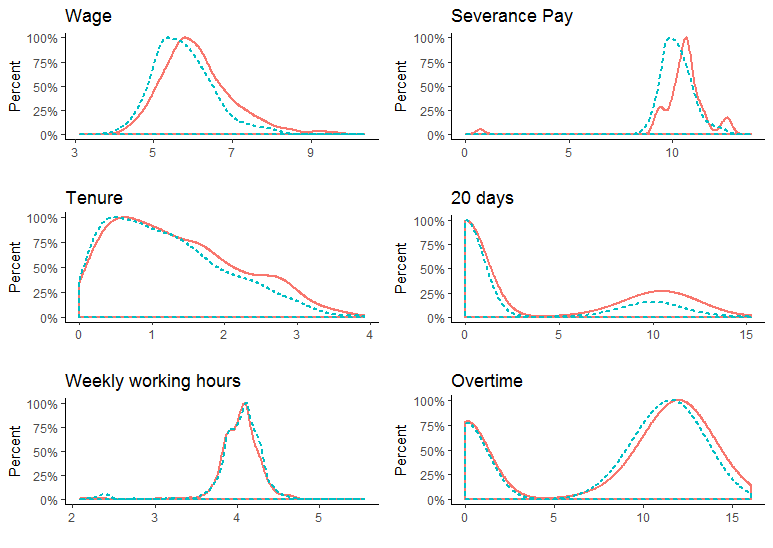
\includegraphics[width=\textwidth]{covariates_continuous.tiff}
        \end{subfigure}
        \begin{subfigure}{0.49\textwidth}
            \caption{Categorical variables}
            \centering
            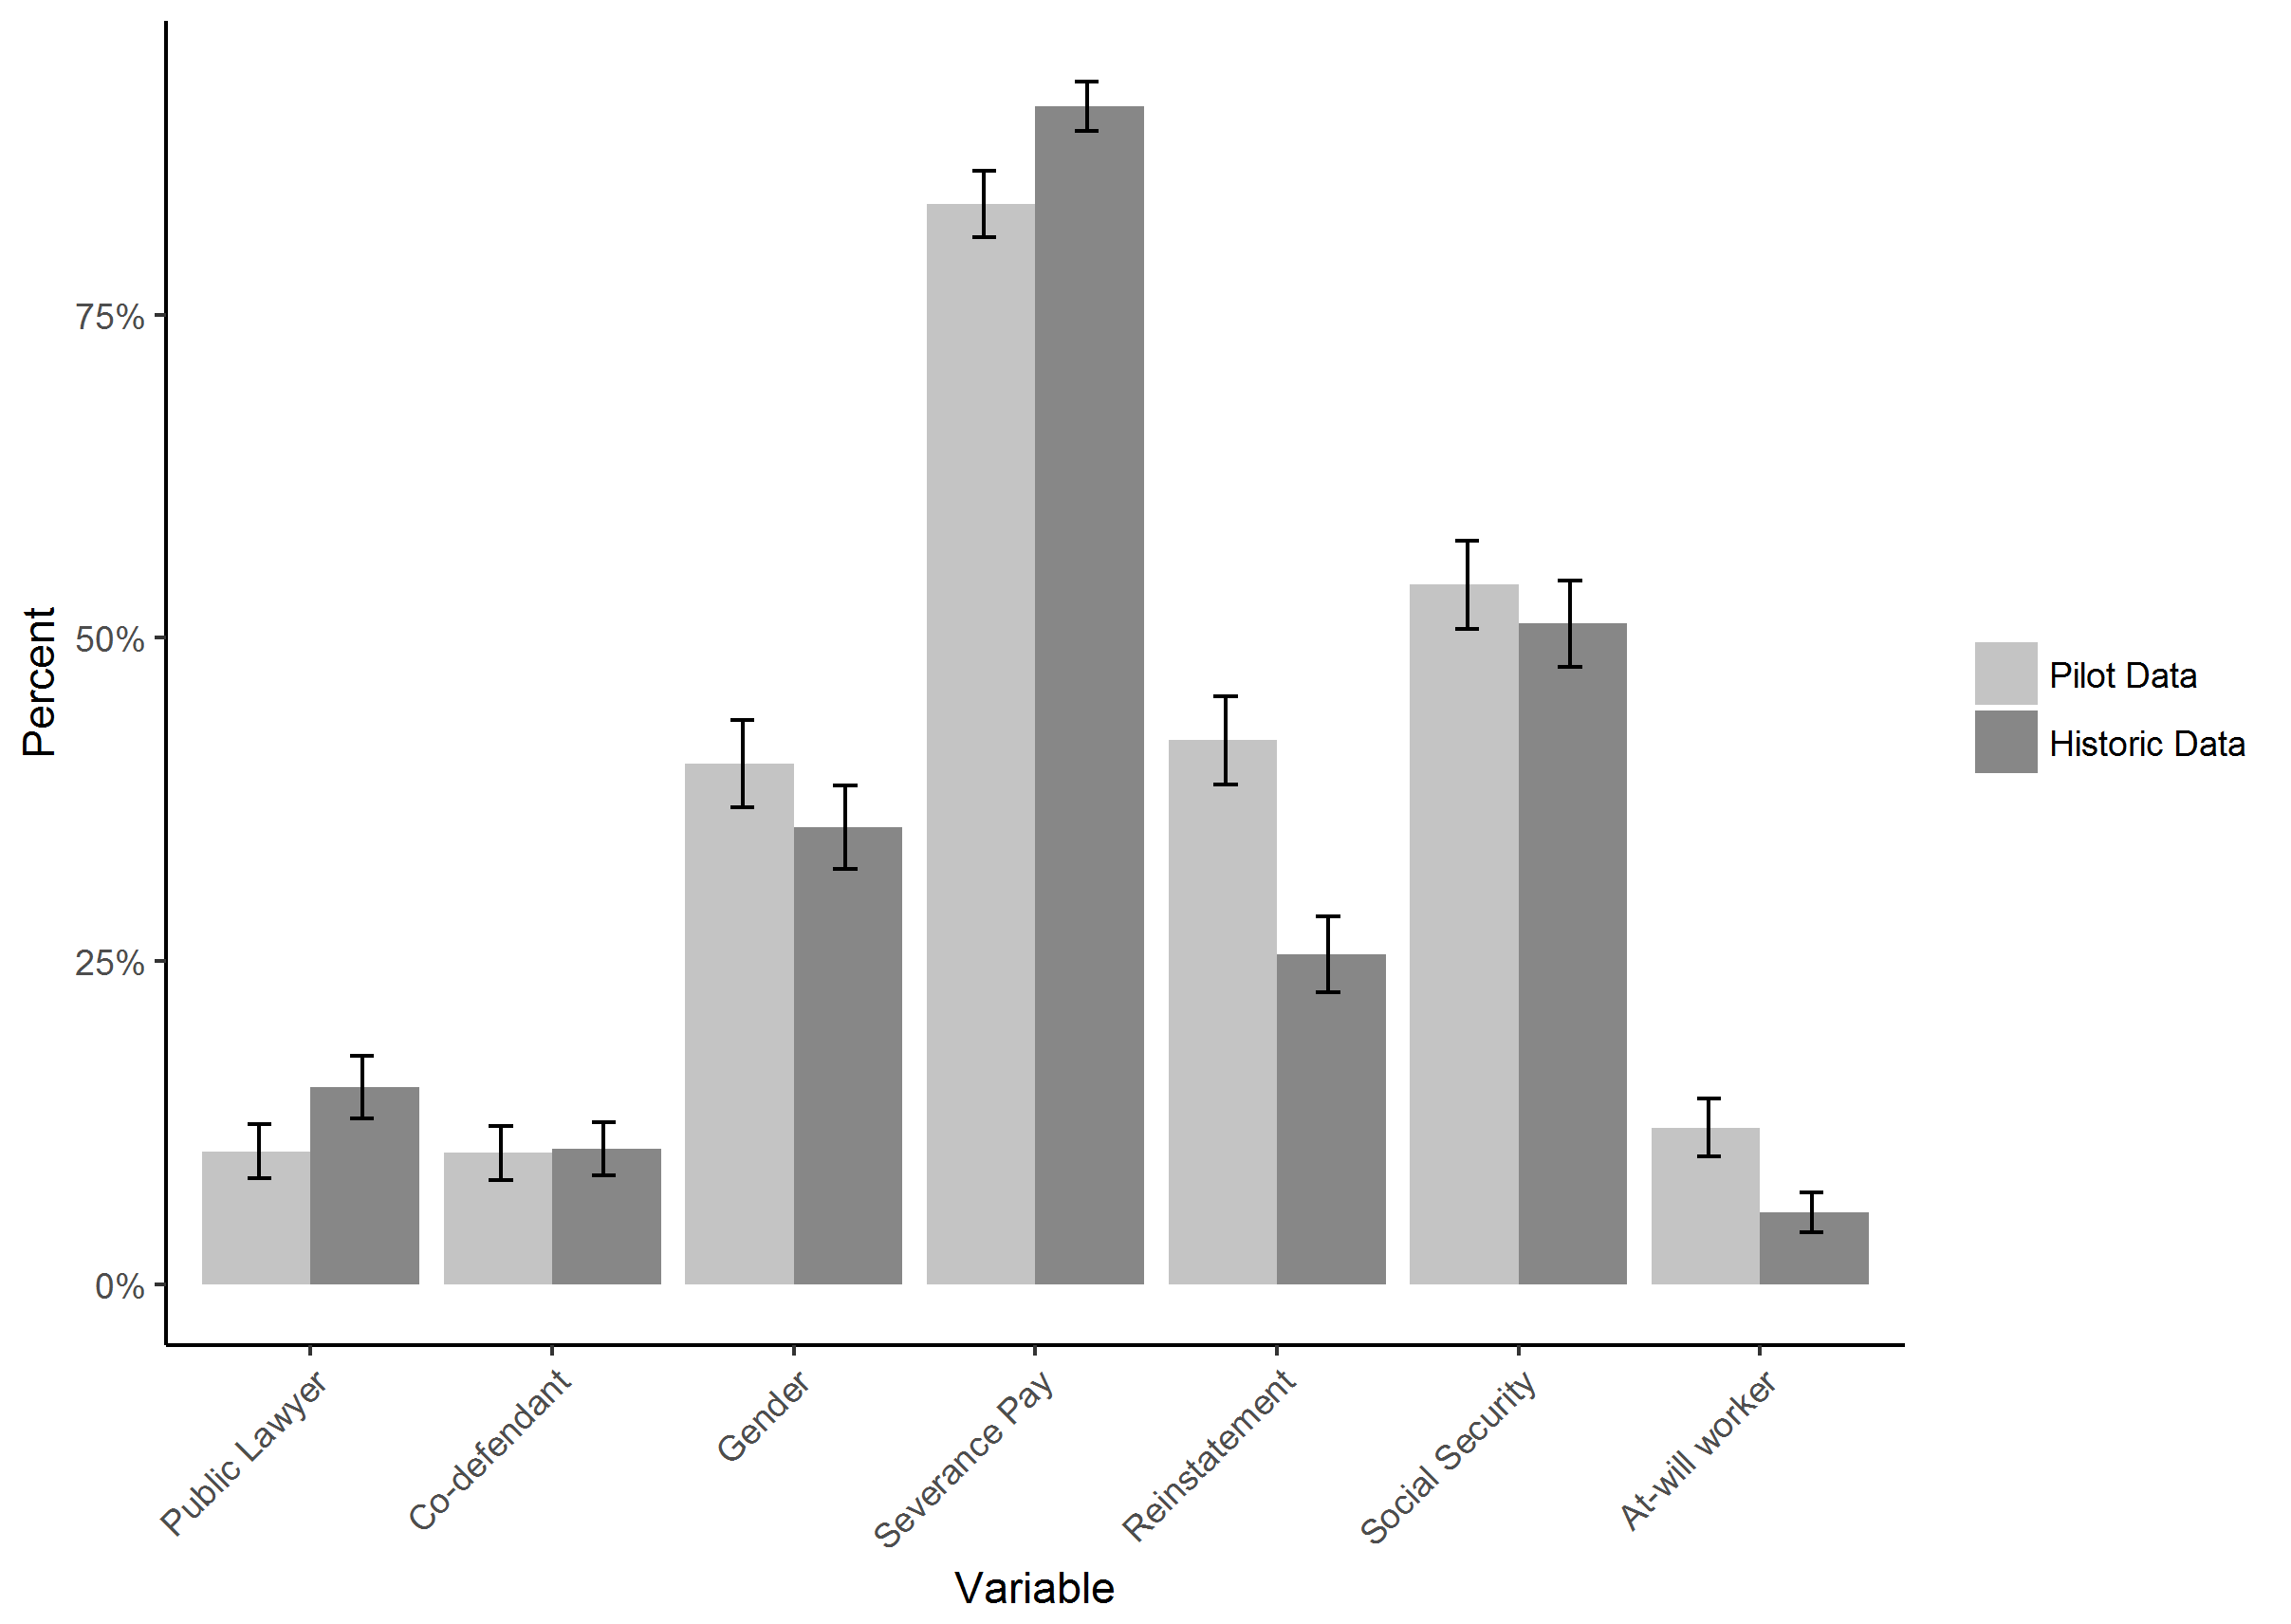
\includegraphics[width=\textwidth]{covariates_categorical.tiff}
        \end{subfigure}
    \end{center}
    {\footnotesize \textit{Notes: } Covariate distributions for historical -used to calibrate our calculator- and pilot data. All continuous variables are plotted in logs. Color guide is the same for both variable types.}
    {\footnotesize \textit{Script: } \texttt{covariate\_plots.R}}
\end{figure}

\begin{figure}[H]
    \caption{Percent that know main legal constitutional entitlement}
    \label{Knowindemfig}
    \begin{center}
        \begin{subfigure}{0.49\textwidth}
            \caption{Employee claims to know}
            \centering
            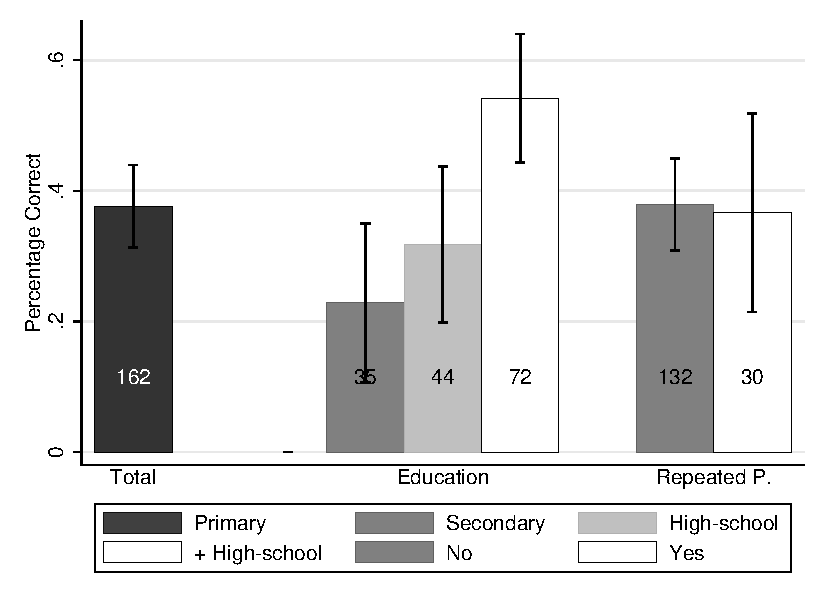
\includegraphics[width=\textwidth]{Knows.pdf}
        \end{subfigure}
        \begin{subfigure}{0.49\textwidth}
            \caption{Employee correctly knows }
                \centering
                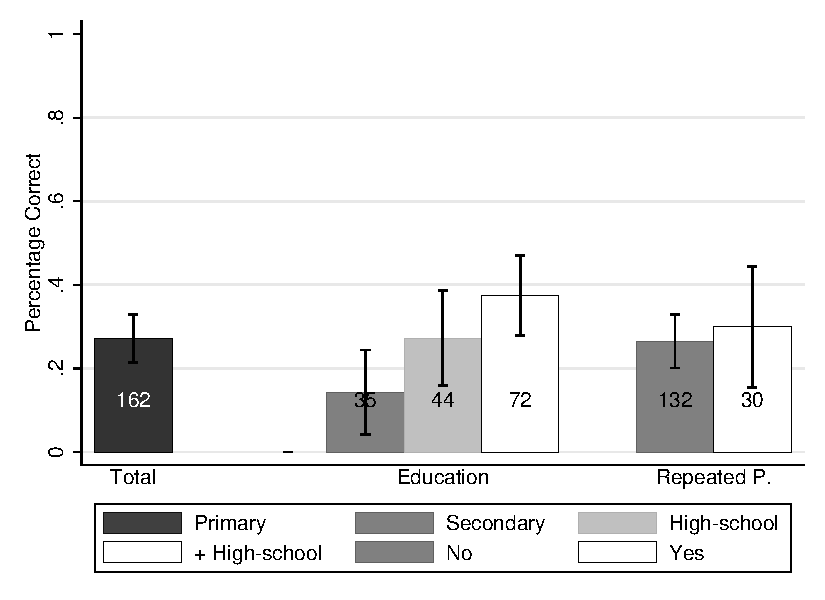
\includegraphics[width=\textwidth]{Correctly_knows.pdf}
        \end{subfigure}
        \end{center}
    {\footnotesize \textit{Notes: } This is based on the subject's answer to two questions: 7.01: "In case of an unjustified firing, the law grants you to get a severance pay stipulated in the Constitution. Do you know how many days of your salary does this account for?" and "7:02: How many days of your salary does this pay account for?". First panel correspond to the first question while second panel to the second one.}
    {\footnotesize \textit{Do file: } \texttt{peiper.do}}
\end{figure}



\begin{figure}[H]
    \caption{Knowledge about their own claims in lawsuit}
    \label{Knowtheirclaimsfig}
    \begin{center}
        \begin{subfigure}{0.49\textwidth}
            \caption{Const. compensation}
            \centering
            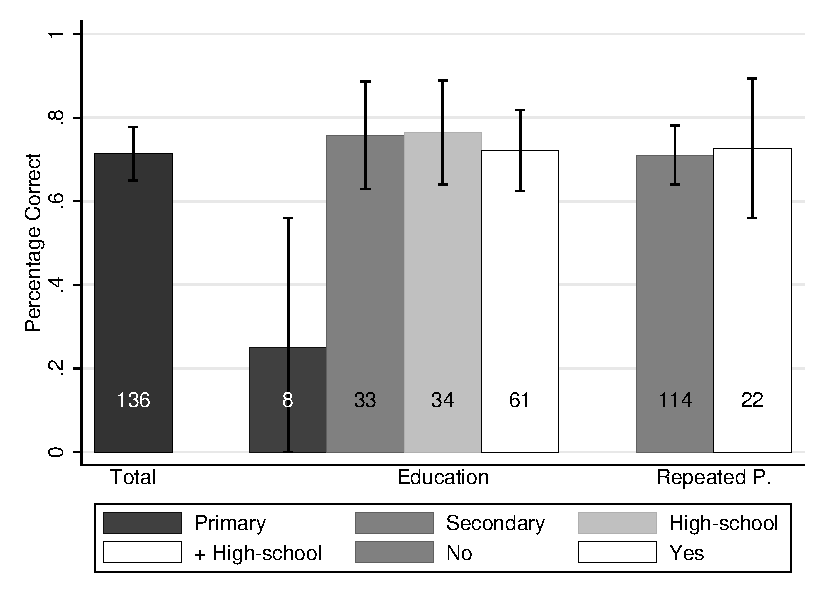
\includegraphics[width=\textwidth]{Compensation.pdf}
        \end{subfigure}
        \begin{subfigure}{0.49\textwidth}
            \caption{SARIMSS}
                \centering
                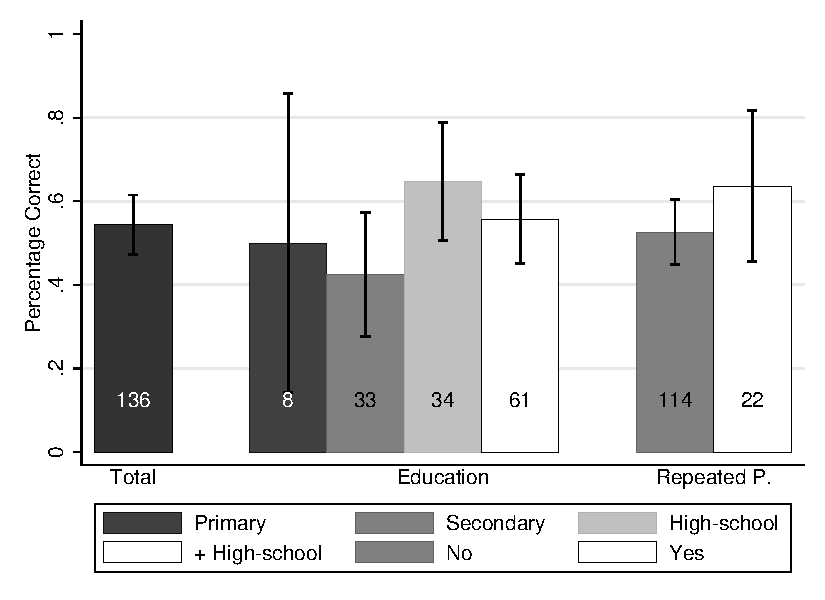
\includegraphics[width=\textwidth]{Insurance.pdf}
        \end{subfigure}
        \begin{subfigure}{0.49\textwidth}
            \caption{Reinstatement}
            \centering
            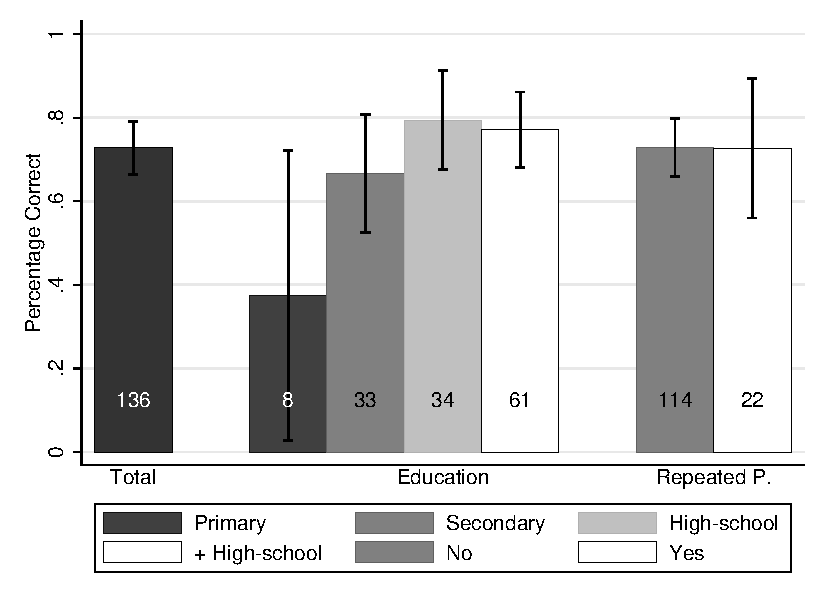
\includegraphics[width=\textwidth]{Reinstatement.pdf}
        \end{subfigure}
            \hfill
        \begin{subfigure}{0.49\textwidth}
            \caption{Overtime}
            \centering
            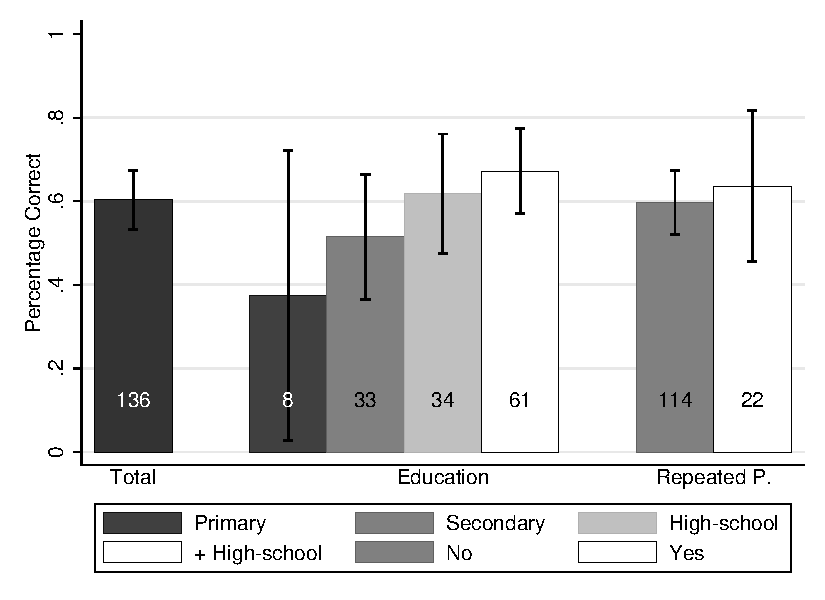
\includegraphics[width=\textwidth]{Extra_hrs.pdf}
        \end{subfigure}
        \begin{subfigure}{0.49\textwidth}
            \caption{End of year bonus}
            \centering
            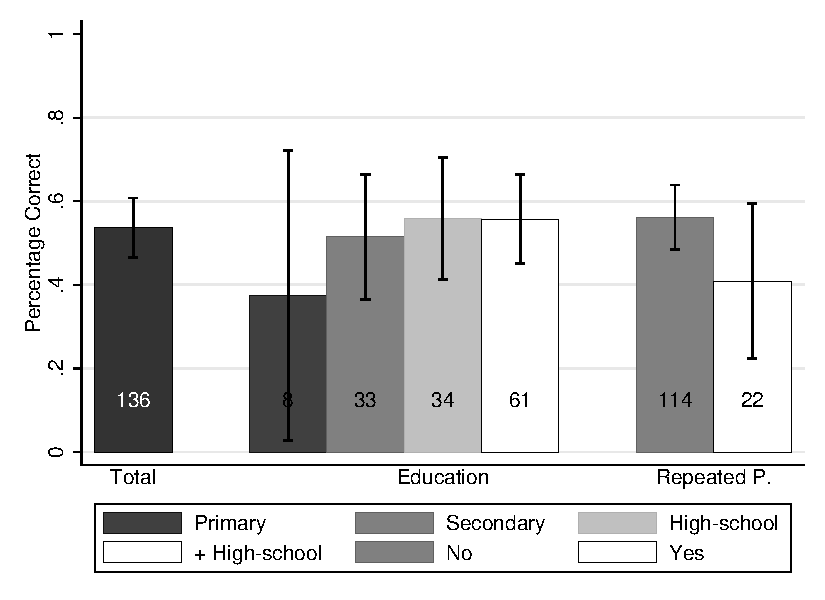
\includegraphics[width=\textwidth]{Holiday_bonus.pdf}
        \end{subfigure}
            \hfill
        \begin{subfigure}{0.49\textwidth}
            \caption{Sunday bonus}
            \centering
            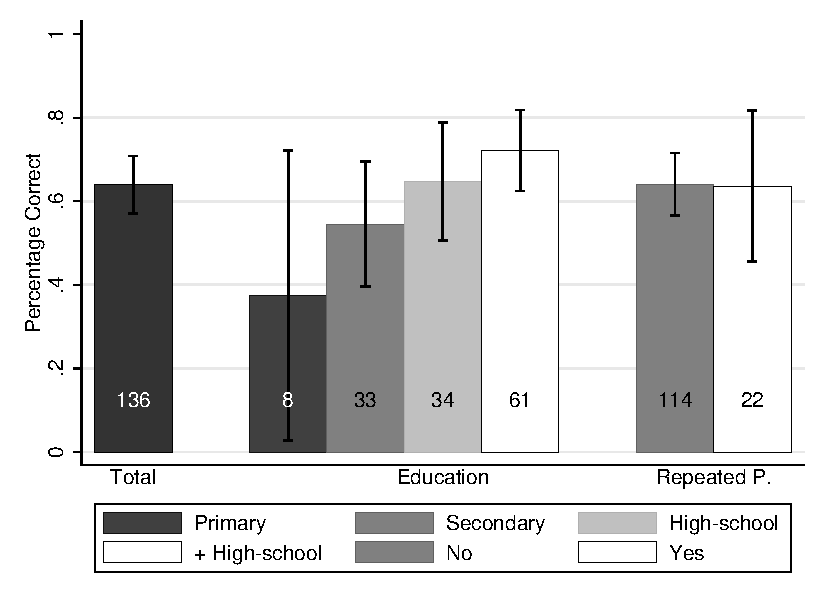
\includegraphics[width=\textwidth]{Sunday_bonus.pdf}
        \end{subfigure}
    \end{center} 
        \footnotesize \textit{Notes: Percentage of subjects who correctly answered to the question regarding elements of their claim, by type of benefit asked.}
        {\footnotesize \textit{Do file: }  \texttt{peiper2.do}}
\end{figure}

 
    
\begin{figure}[H]
    \caption{Differences in claims and compensation by case file outcome}
    \label{claimsvsoutcomes}
    \begin{center}
        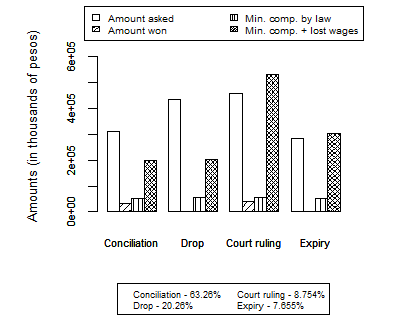
\includegraphics[width=0.7\textwidth]{Amountasked.tiff}
        \end{center}
    \footnotesize \textit{Notes: This graph shows the average amount (in thousand pesos) asked, won (overall and conditional on winning), minimum legal compensation, and minimum legal compensation plus lost wages, by outcome. The bottom legend shows the percentage of cases with each outcome for our database (N=5005). Note that, by definition, workers have no chance of recovery in drops and expiries. In our data, all settlements imply a positive recovery for the worker; finally, \textbf{for judgments, only 24\% of the time does the worker recover anything.}} 
    {\footnotesize \textit{Script: } \texttt{amount\_plots.R}}
\end{figure}


  
\begin{figure}[H]
    \caption{Delay of case by type of conclusion}
    \label{DurationFig}
    \begin{center}
        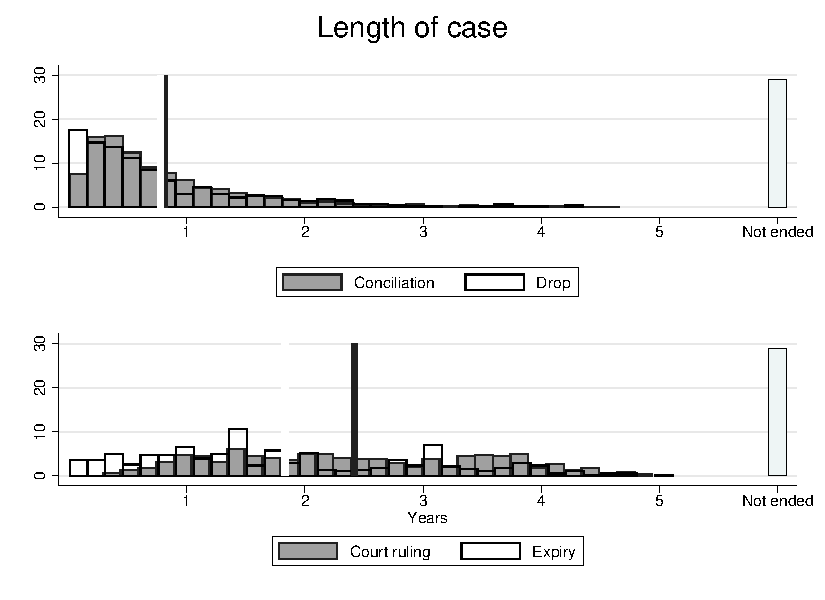
\includegraphics[width=0.7\textwidth]{Duracion.pdf}
        \end{center}
    {\footnotesize \textit{Notes: Length of the case (in years) , by conclusion. Naturally, laudos (adjudication cases) have much higher duration than settlement cases (convenios).}}
    {\footnotesize \textit{Do file: } \texttt{peiper5.do}}
\end{figure}



\begin{figure}[H]
    \caption{Difference in what actor says and calculator predicts in amount and probability.}
    \label{Figure_overconfidence_exp}
    \begin{center}
    \begin{subfigure}{0.49\textwidth}
        \caption{Employee}
        \centering
        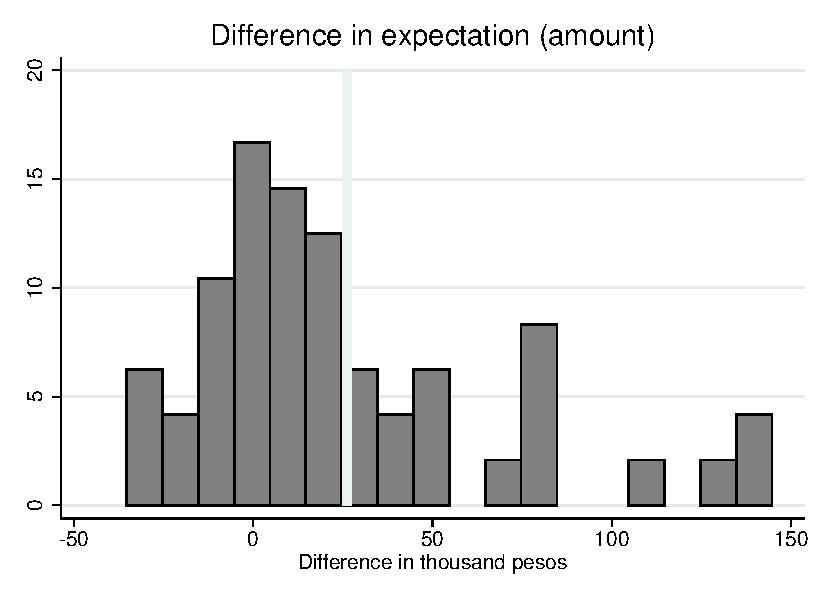
\includegraphics[width=\textwidth]{difference_amount_employee.pdf}
    \end{subfigure}
     \begin{subfigure}{0.49\textwidth}
        \centering
        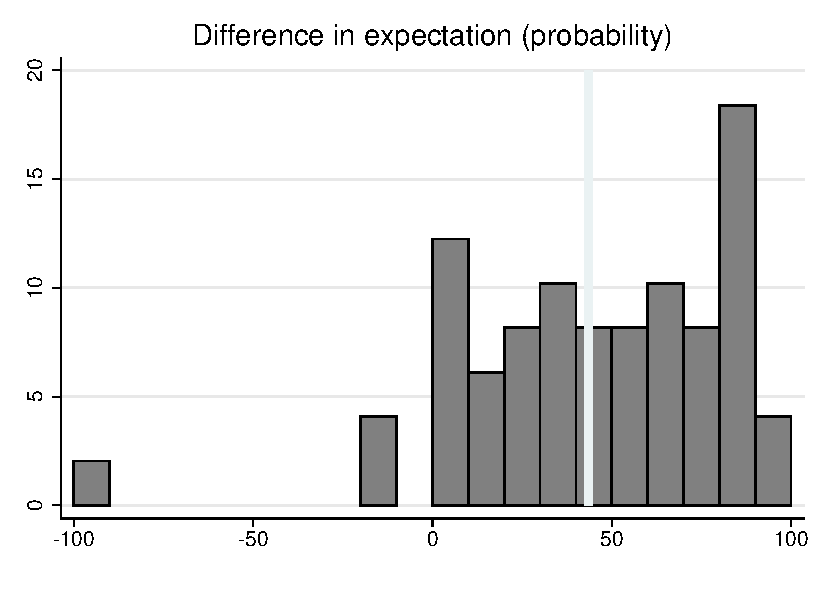
\includegraphics[width=\textwidth]{difference_prob_employee.pdf}
    \end{subfigure}
    \begin{subfigure}{0.49\textwidth}
        \caption{Employee Lawyer}
        \centering
        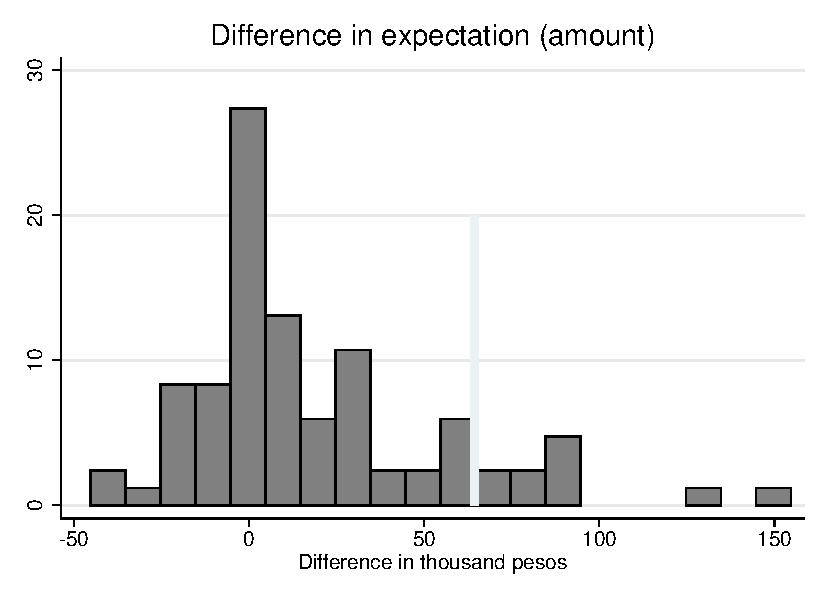
\includegraphics[width=\textwidth]{difference_amount_employeelawyer.pdf}
        \end{subfigure}
          \begin{subfigure}{0.49\textwidth}
        \centering
        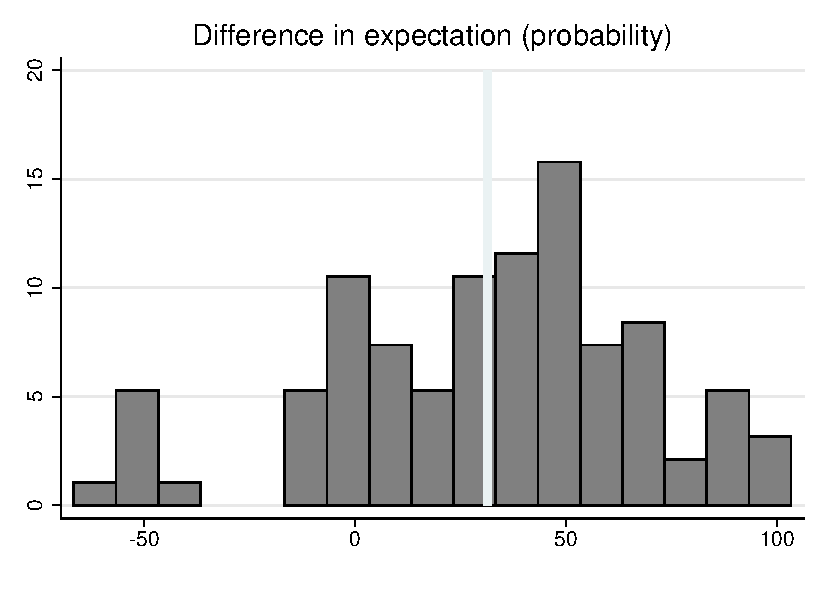
\includegraphics[width=\textwidth]{difference_prob_employeelawyer.pdf}
    \end{subfigure}
        \begin{subfigure}{0.49\textwidth}
            \caption{Firm Lawyer}
            \centering
            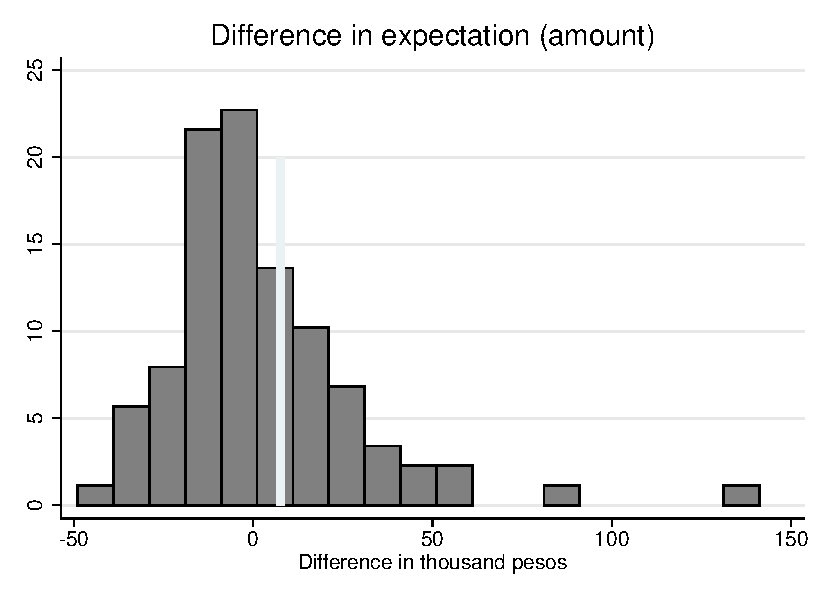
\includegraphics[width=\textwidth]{difference_amount_firmlawyer.pdf}
    \end{subfigure}
    \begin{subfigure}{0.49\textwidth}
            \centering
            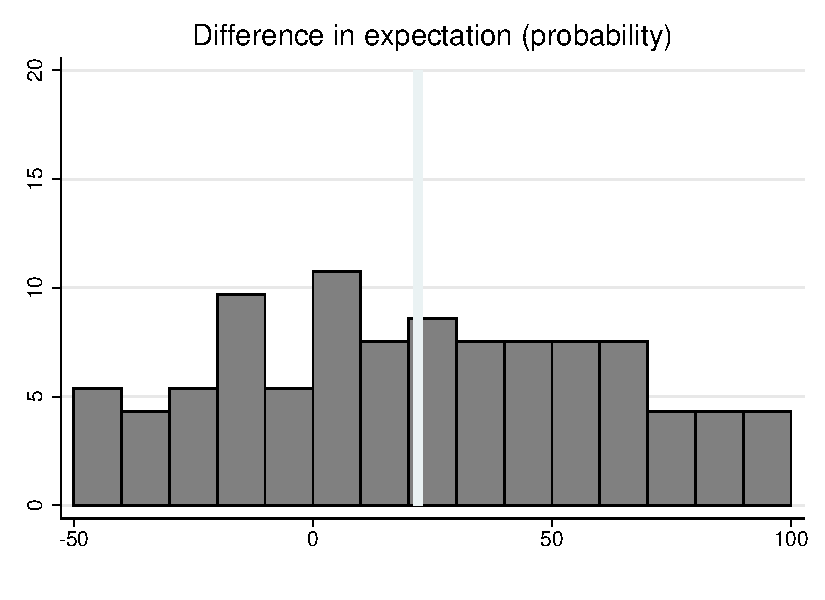
\includegraphics[width=\textwidth]{difference_prob_firmlawyer.pdf}
        \end{subfigure}
    \end{center}
     \footnotesize \textit{Notes: Difference (in thousand pesos for amounts, percentage points for probabilities) from what the subject expects vs. what our models predict. Note how, for Employee and employee lawyer, the distribution for amounts is much more skewed to the right than for firm lawyers. This is only natural, since the formers are thinking about expected wins and the latters about expected losses.} 
      \footnotesize{ \textit{Do file: }  \texttt{oc\_comparison\_B.do}}
\end{figure}



\begin{figure}[H]
   \caption{Experiment flowchart}
   \label{treatment_flowchart}
    \begin{center}
    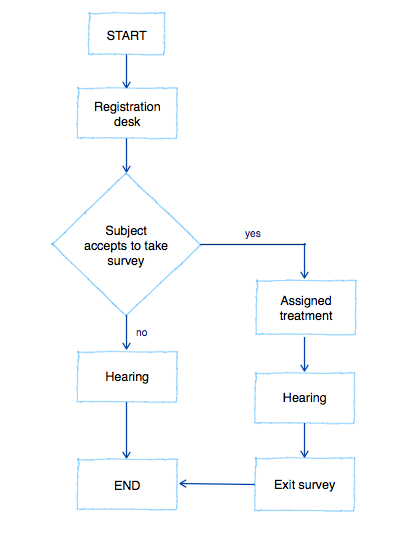
\includegraphics[width=0.42\textwidth]{./Figuras/Experiment_flowchart.png}
    \end{center}
    \footnotesize
    \textit{Notes: this flowchart shows what happened when subjects arrived to the court.}
\end{figure}
    



\begin{figure}[H]
    \caption{Calculator treatment format (example)}
    \label{calc_template}
    \begin{center}
        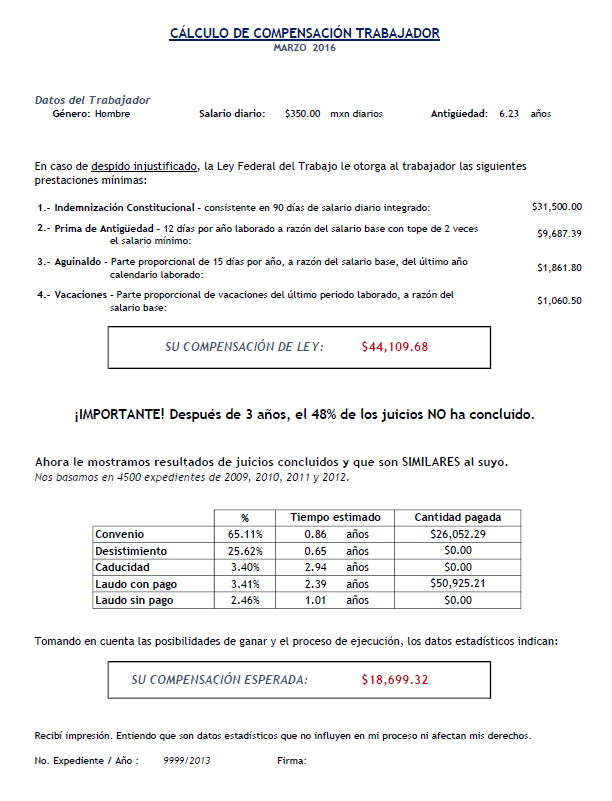
\includegraphics[width=0.9\textwidth]{calctreat.png}
        \end{center}
        {\footnotesize \textit{Notes: An example of the format shown to subjects in calculator treatment group. It shows some data on the worker, the minimum legal amount she deserves for different types of benefits, a small note on average trial duration, and calculator results: probability for each conclusion outcome, average duration and amount won (both conditional on each outcome).}}
\end{figure}




\begin{figure}[H]
    \caption{Belief updating after treatment}
    \label{Figure_updating}
    \begin{center}
%    \begin{subfigure}{\textwidth}
%        \caption{update in beliefs in duration}
%        \centering
%        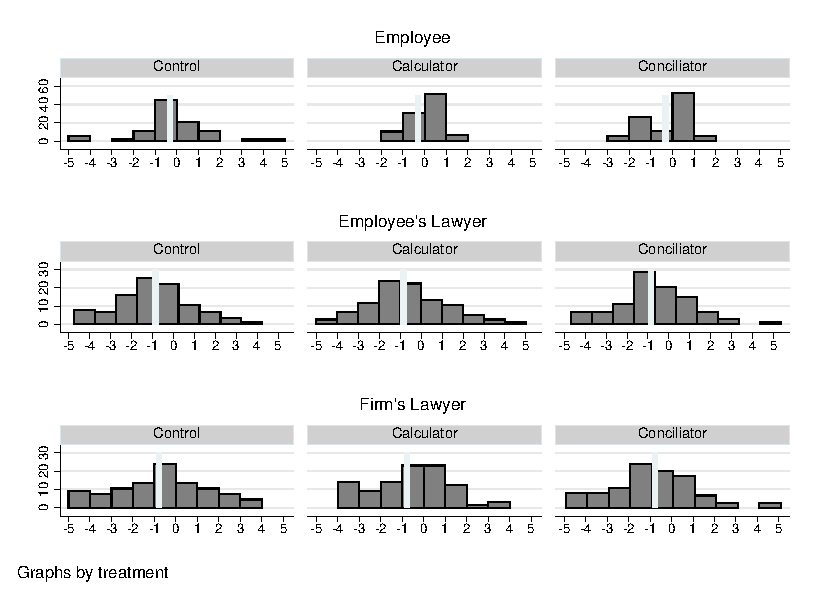
\includegraphics[width=\textwidth]{updatebeleif_duration.pdf}
%    \end{subfigure}
    \begin{subfigure}{\textwidth}
        \caption{Update in beliefs in amount}
        \centering
        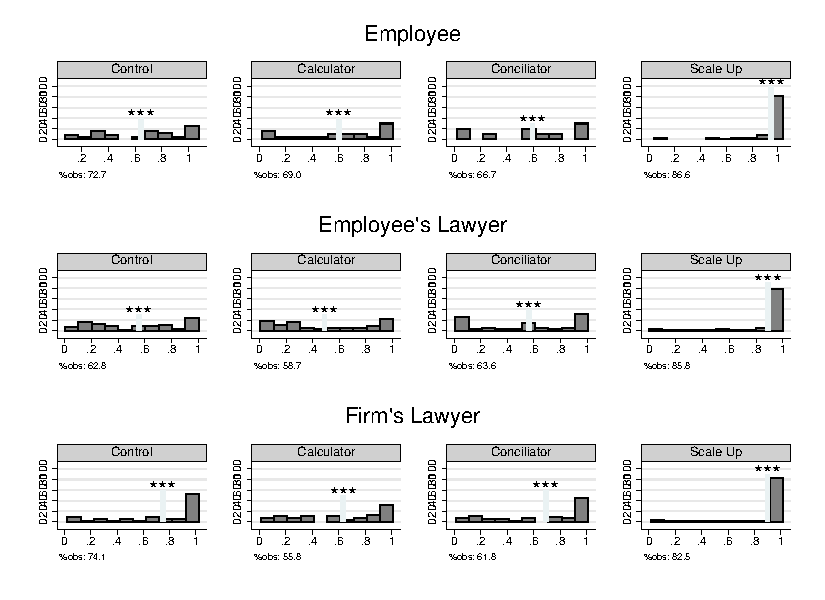
\includegraphics[width=\textwidth]{updatebeleif_amount.pdf}
    \end{subfigure}
    \end{center}
     \footnotesize \textit{Notes: Graphs on belief updating. They show the following statistic: $\theta=\left|\frac{P-exitsurvey}{P-initialsurvey}\right|$. Where $P$ is the prediction made by the calculator and $exit$ and $initial$ survey variables denote what each part answered on the survey for amount won. Note that when $\theta=1$ we have no update with respect to the prediction. And when $\theta<1$ they update in the direction of what calculator says. The extreme case $\theta=0$ implies perfect updating with respect to what the calculator says.} 
      \footnotesize{ \textit{Do file: }  \texttt{Update\_beleifs.do}}
\end{figure}


      
\begin{figure}[H]
    \caption{Conciliation over time}
    \label{Figure_dynamicsConciliation}
    \begin{center}
    \begin{subfigure}{0.49\textwidth}
    \centering
        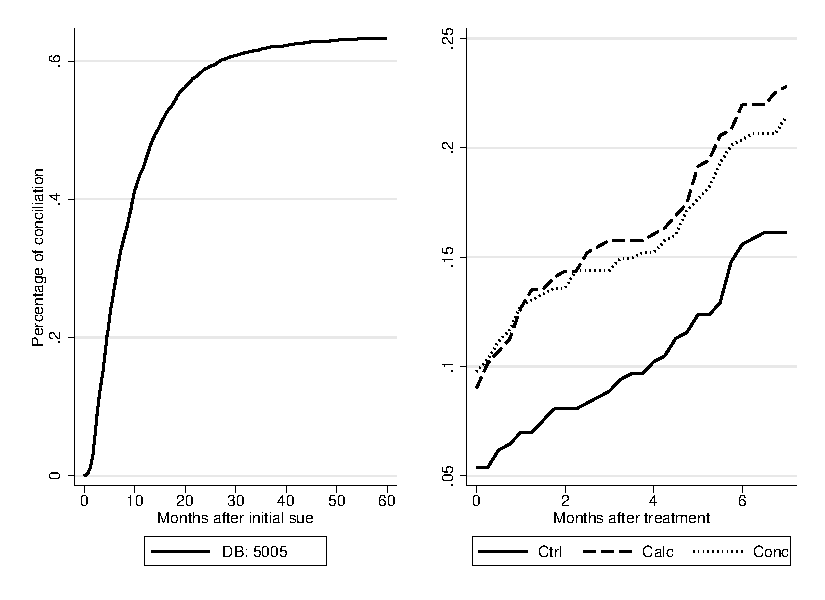
\includegraphics[width=1\textwidth]{con_overtime.pdf}
     \end{subfigure}
        \begin{subfigure}{0.49\textwidth}    
         \centering
        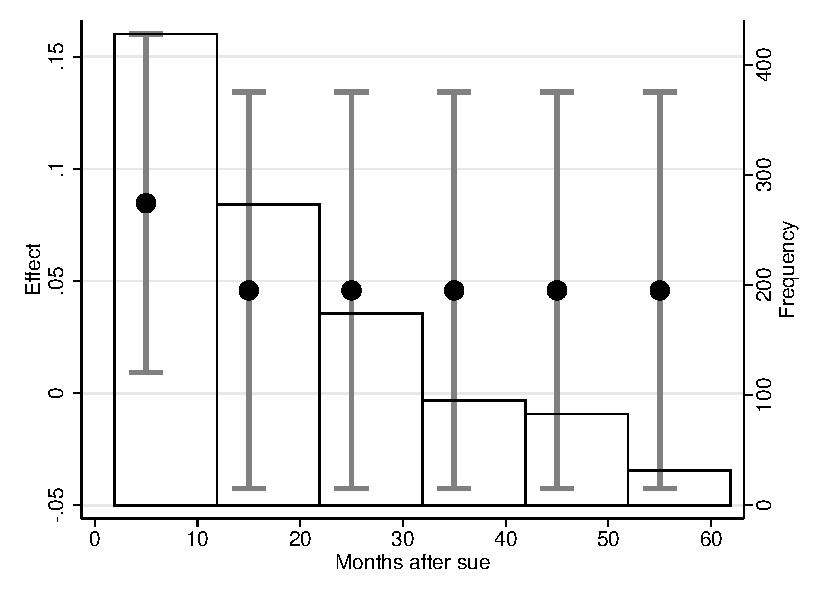
\includegraphics[width=1\textwidth]{beta_monthsafter.pdf}
     \end{subfigure}
        \end{center}
        {\footnotesize \textit{Notes: } Conciliation over time in HD database and pilot database. Figure on the right shows the effect of conciliation on treated against control for different months after initial sue.}
        {\footnotesize \textit{Do file: } \texttt{con\_overtime.do , beta\_monthsafter.do}}
\end{figure}



%%%%%%%%%%%%%%%%%%%%%%%%%%%%%%%%%%%%%%%%%%%%%%%

% APPENDIX TABLES

\section{APPENDIX}

\subsection{Tables}



\begin{table}[H]
    \caption{Variable list description }
    \label{tab:SS}
    \begin{center}
        \scriptsize{% Table generated by Excel2LaTeX from sheet 'Variable_list'
\begin{tabular}{p{2cm}p{12cm}}
\toprule
\multicolumn{1}{l}{\textbf{VARIABLE}} & \multicolumn{1}{l}{\textbf{DESCRIPTION}} \\
\midrule
\midrule
\textbf{Public Lawyer*} & If the lawyer is public or private. \\
\textbf{Female*} & Dummy for female plaintiff. \\
\textbf{At will worker*} & If the worker is an at will employee. \\
\textbf{Tenure*} & Employee's tenure with the employer. \\
\textbf{Daily wage*} & Daily salary. \\
\textbf{Weekly hours*} & Number of hours that the plaintiff worked on a weekly basis. \\
\textbf{Reinstatement*} & If the plaintiff claims reinstatement. \\
\textbf{Severance pay*} & If the plaintiff claims constitutional indemnity (three months of integrated salary) that the law dictates for unjustified dismissal. \\
\textbf{Lost wages*} & If the plaintiff claims lost wages/back pay. \\
\textbf{Tenure bonus} & If the plaintiff claims the payment of "tenure bonus" (12 days per year worked, up to two times minimum wage). \\
\textbf{End of year bonus} & If the plaintiff claims end of year bonus. \\
\textbf{Vacation pay} & If the plaintiff claims accrued vacation days not taken. \\
\textbf{Overtime*} & If the plaintiff claims overtime pay. \\
\textbf{Twenty days x year*} & If the plaintiff claims the payment of compensation (20 days per year worked) that the law dictates for unjustified dismissal for a worker who has the right to be reinstated but the employer refuses to reinstate, or for an at-will employee who cannot ask for reinstatement. \\
\textbf{Sunday bonus} & If the plaintiff claims the payment of bonus for working on Sundays (the law provides for a 25\% premium for working Sundays). \\
\textbf{Weekly rest} & If the plaintiff claims the payment of weekly rest day (3 times daily wage). \\
\textbf{Compulsory rest} & If the plaintiff claims the payment of legal holidays worked (3 times daily wage). \\
\textbf{Profit sharing} & If the plaintiff claims the proportional payment of profits generated by the company that correspond under the labor law to employees. \\
\textbf{SARIMSS*} & If the plaintiff claims the payment of employer contributions that were not made to these institutions, or retroactive registration in the institutions (SAR: retirement savings, IMSS: social security, INFONAVIT: worker's housing fund). \\
\textbf{Nullification of documents} & If the plaintiff requests the nullification of documents, including for example a signed letter of resignation that the worker was made to sign as a blank page, upon being hired, and which later was filled out by the employer with the text of a voluntary letter of resignation. \\
\textbf{Co-defendant*} & If at least one of the codefendants is the IMSS or INFONAVIT or SAR. \\
\textbf{Total asked} & The total quantifiable peso amount of the worker's claim. \\
\textbf{Industry*} & Defendants industry coded as the North American Industry Classification System (NAICS), which provides a consistent framework to classify companies and business establishments to allow for a high level of comparability in business statistics among the North American countries. \\
\bottomrule
\bottomrule
\end{tabular}%
}
    \end{center}
    \footnotesize
    \textit{Notes:} 
Detailed description of variables used throughout the paper. The variables marked with \textbf{*} are the ones that made it to the final model.
\end{table}


\begin{table}[H]
    \caption{Baseline Expectations}
    \label{Table_expectations}
    \begin{center}
       \scriptsize{% Table generated by Excel2LaTeX from sheet 'SS_A'
\begin{tabular}{rrrr}
\toprule
      & \multicolumn{1}{c}{Total} & \multicolumn{1}{c}{Public Lawyer} & \multicolumn{1}{c}{Private Lawyer} \\
\midrule
\multicolumn{1}{l}{Variable} & \multicolumn{3}{c}{Employee} \\
\midrule
\midrule
\multicolumn{1}{l}{Prob winning} & \multicolumn{1}{l}{.8} & \multicolumn{1}{l}{.79} & \multicolumn{1}{l}{.8} \\
\multicolumn{1}{l}{} & \multicolumn{1}{l}{(.23)} & \multicolumn{1}{l}{(.23)} & \multicolumn{1}{l}{(.23)} \\
\multicolumn{1}{l}{Most prob amount} & \multicolumn{1}{l}{75478.14} & \multicolumn{1}{l}{37543.06} & \multicolumn{1}{l}{89134.77} \\
\multicolumn{1}{l}{} & \multicolumn{1}{l}{(263891)} & \multicolumn{1}{l}{(54321.51)} & \multicolumn{1}{l}{(305297.61)} \\
\multicolumn{1}{l}{Most prob duration} & \multicolumn{1}{l}{2.68} & \multicolumn{1}{l}{2.58} & \multicolumn{1}{l}{2.72} \\
\multicolumn{1}{l}{} & \multicolumn{1}{l}{(1.74)} & \multicolumn{1}{l}{(1.97)} & \multicolumn{1}{l}{(1.65)} \\
\multicolumn{1}{l}{Obs} & \multicolumn{1}{l}{136} & \multicolumn{1}{l}{36} & \multicolumn{1}{l}{98} \\
\midrule
\multicolumn{1}{l}{} & \multicolumn{3}{c}{Employee's Lawyer} \\
\midrule
\midrule
\multicolumn{1}{l}{Prob winning} & \multicolumn{1}{l}{.73} & \multicolumn{1}{l}{.62} & \multicolumn{1}{l}{.74} \\
\multicolumn{1}{l}{} & \multicolumn{1}{l}{(.2)} & \multicolumn{1}{l}{(.19)} & \multicolumn{1}{l}{(.2)} \\
\multicolumn{1}{l}{Most prob amount} & \multicolumn{1}{l}{214904.55} & \multicolumn{1}{l}{38127} & \multicolumn{1}{l}{233710.68} \\
\multicolumn{1}{l}{} & \multicolumn{1}{l}{(1291234.24)} & \multicolumn{1}{l}{(81074.83)} & \multicolumn{1}{l}{(1356804.44)} \\
\multicolumn{1}{l}{Most prob duration} & \multicolumn{1}{l}{3.67} & \multicolumn{1}{l}{5.41} & \multicolumn{1}{l}{3.48} \\
\multicolumn{1}{l}{} & \multicolumn{1}{l}{(1.9)} & \multicolumn{1}{l}{(2.35)} & \multicolumn{1}{l}{(1.75)} \\
\multicolumn{1}{l}{Obs} & \multicolumn{1}{l}{312} & \multicolumn{1}{l}{30} & \multicolumn{1}{l}{282} \\
\midrule
\multicolumn{1}{l}{} & \multicolumn{3}{c}{Firm's Lawyer} \\
\midrule
\midrule
\multicolumn{1}{l}{Prob winning} & \multicolumn{1}{l}{0.68} & \multicolumn{1}{l}{.74} & \multicolumn{1}{l}{.67} \\
\multicolumn{1}{l}{} & \multicolumn{1}{l}{(.22)} & \multicolumn{1}{l}{(.22)} & \multicolumn{1}{l}{(.22)} \\
\multicolumn{1}{l}{Most prob amount} & \multicolumn{1}{l}{58052.43} & \multicolumn{1}{l}{13035.84} & \multicolumn{1}{l}{62539.61} \\
\multicolumn{1}{l}{} & \multicolumn{1}{l}{(239962.38)} & \multicolumn{1}{l}{(15724.8)} & \multicolumn{1}{l}{(251183.91)} \\
\multicolumn{1}{l}{Most prob duration} & \multicolumn{1}{l}{4.07} & \multicolumn{1}{l}{3.45} & \multicolumn{1}{l}{4.13} \\
\multicolumn{1}{l}{} & \multicolumn{1}{l}{(2.11)} & \multicolumn{1}{l}{(1.67)} & \multicolumn{1}{l}{(2.14)} \\
\multicolumn{1}{l}{Obs} & \multicolumn{1}{l}{342} & \multicolumn{1}{l}{31} & \multicolumn{1}{l}{311} \\
\bottomrule
\bottomrule
\end{tabular}%
}
    \end{center}
    \footnotesize    
    \textit{Notes:} 
    Summary statistics of parties' beliefs. We show mean and standard deviation for the whole sample, \& dividing by type of employee's lawyer.
    \textit{Do file: } \texttt{Table\_SS.do  Table\_SS\_bylawyer.do}
\end{table}

%\pagebreak
%\begin{center}
%    \tiny{
\begin{table}[htbp]\centering \caption{SS survey variables \label{sumstat}}
\begin{tabular}{l c c c c c}\hline\hline
\multicolumn{1}{c}{\textbf{Variable}} & \textbf{Mean}
 & \textbf{Std. Dev.}& \textbf{Min.} &  \textbf{Max.} & \textbf{N}\\ \hline
Initial prob employee & 79.812 & 24.906 & 10 & 100 & 223\\
Initial amount employee & 62736.224 & 87655.907 & 0 & 600000 & 188\\
Exit prob employee & 71.076 & 28.445 & 10 & 100 & 171\\
Exit amount employee & 54801.663 & 66298.621 & 0 & 350000 & 142\\
Initial prob employee's lawyer & 77.762 & 20.026 & 2 & 100 & 965\\
Initial amount employee's lawyer & 97572.459 & 112949.152 & 0 & 700000 & 768\\
Exit prob employee's lawyer & 67.505 & 24.514 & 1 & 100 & 733\\
Exit amount employee's lawyer & 87234.616 & 96300.243 & 0 & 600000 & 568\\
Initial prob firm's lawyer & 40.363 & 22.95 & 1 & 100 & 584\\
Initial amount firm's lawyer & 59030.199 & 82031.346 & 0 & 662451 & 462\\
Exit prob firm's lawyer & 42.416 & 23.352 & 1 & 100 & 440\\
Exit amount firm's lawyer & 56965.815 & 70131.048 & 0 & 480001 & 363\\
Buys goods & 0.074 & 0.263 & 0 & 1 & 229\\
Works & 0.426 & 0.496 & 0 & 1 & 230\\
Looking for a job & 0.551 & 0.498 & 0 & 1 & 225\\
\hline\end{tabular}
\end{table}
}
%\end{center}
%\vspace{5mm}
%    \footnotesize
 %   \textit{Notes:} 
%Summary stats of survey variables for employee, employee's lawyer and firm's lawyer
%    \textit{Do file: } \texttt{}
% \pagebreak


\begin{table}[H]
    \caption{Who showed up }
    \label{whoshowedup}
    \begin{center}
        \scriptsize{% Table generated by Excel2LaTeX from sheet 'Showed_up'
\begin{tabular}{rrrr}
\toprule
      & \multicolumn{1}{c}{Control} & \multicolumn{1}{c}{Calculator} & \multicolumn{1}{c}{Conciliator} \\
\midrule
\multicolumn{1}{l}{No one showed up} & \multicolumn{1}{l}{0.071} & \multicolumn{1}{l}{0.077} & \multicolumn{1}{l}{0.050} \\
\multicolumn{1}{l}{E} & \multicolumn{1}{l}{0.003} & \multicolumn{1}{l}{0.006} & \multicolumn{1}{l}{0.000} \\
\multicolumn{1}{l}{L} & \multicolumn{1}{l}{0.134} & \multicolumn{1}{l}{0.120} & \multicolumn{1}{l}{0.134} \\
\multicolumn{1}{l}{F} & \multicolumn{1}{l}{0.000} & \multicolumn{1}{l}{0.000} & \multicolumn{1}{l}{0.000} \\
\multicolumn{1}{l}{D} & \multicolumn{1}{l}{0.068} & \multicolumn{1}{l}{0.080} & \multicolumn{1}{l}{0.100} \\
\multicolumn{1}{l}{EL} & \multicolumn{1}{l}{0.041} & \multicolumn{1}{l}{0.023} & \multicolumn{1}{l}{0.017} \\
\multicolumn{1}{l}{EF} & \multicolumn{1}{l}{0.000} & \multicolumn{1}{l}{0.000} & \multicolumn{1}{l}{0.000} \\
\multicolumn{1}{l}{ED} & \multicolumn{1}{l}{0.011} & \multicolumn{1}{l}{0.000} & \multicolumn{1}{l}{0.006} \\
\multicolumn{1}{l}{LF} & \multicolumn{1}{l}{0.000} & \multicolumn{1}{l}{0.003} & \multicolumn{1}{l}{0.000} \\
\multicolumn{1}{l}{LD} & \multicolumn{1}{l}{0.516} & \multicolumn{1}{l}{0.521} & \multicolumn{1}{l}{0.540} \\
\multicolumn{1}{l}{FD} & \multicolumn{1}{l}{0.003} & \multicolumn{1}{l}{0.000} & \multicolumn{1}{l}{0.000} \\
\multicolumn{1}{l}{ELF} & \multicolumn{1}{l}{0.005} & \multicolumn{1}{l}{0.000} & \multicolumn{1}{l}{0.000} \\
\multicolumn{1}{l}{ELD} & \multicolumn{1}{l}{0.123} & \multicolumn{1}{l}{0.157} & \multicolumn{1}{l}{0.128} \\
\multicolumn{1}{l}{EFD} & \multicolumn{1}{l}{0.000} & \multicolumn{1}{l}{0.003} & \multicolumn{1}{l}{0.000} \\
\multicolumn{1}{l}{LFD} & \multicolumn{1}{l}{0.016} & \multicolumn{1}{l}{0.006} & \multicolumn{1}{l}{0.017} \\
\multicolumn{1}{l}{ELFD} & \multicolumn{1}{l}{0.008} & \multicolumn{1}{l}{0.006} & \multicolumn{1}{l}{0.008} \\
\bottomrule
\end{tabular}%
}
    \end{center}
    \footnotesize
    \textit{Notes:} 
We show some stats of who goes to the court. This is important since we can only give the treatment to the parties who go.  We decompose this in all the possible combination of show up: we use E,L,F,D subscripts to denote the different parties E: Employee; L: Employee’s Lawyer;  F: Firm; D: Firm’s Lawyer.
    \textit{Do file: } \texttt{.do}
\end{table}







%#appendix
\begin{table}[H]
    \caption{Conciliation by type of lawyer}
    \label{tab:reg_con_oc}
    \begin{center}
        \scriptsize{% Table generated by Excel2LaTeX from sheet 'concilio_vs_lawyer'
\begin{tabular}{rrrrr}
\toprule
      & \multicolumn{2}{c}{Conciliation} & \multicolumn{2}{c}{\# months after initial sue} \\
\midrule
      & \multicolumn{1}{c}{(1)} & \multicolumn{1}{c}{(2)} & \multicolumn{1}{c}{(1)} & \multicolumn{1}{c}{(2)} \\
      \midrule
\multicolumn{1}{l}{Public Lawyer} & \multicolumn{1}{l}{0.877} & \multicolumn{1}{l}{-0.817} & \multicolumn{1}{l}{0.0326} & \multicolumn{1}{l}{1.178**} \\
\multicolumn{1}{l}{} & \multicolumn{1}{l}{(2.297)} & \multicolumn{1}{l}{(2.703)} & \multicolumn{1}{l}{(0.492)} & \multicolumn{1}{l}{(0.600)} \\
\multicolumn{1}{l}{Female} & \multicolumn{1}{l}{4.187***} & \multicolumn{1}{l}{4.396***} & \multicolumn{1}{l}{-0.279} & \multicolumn{1}{l}{-0.311} \\
\multicolumn{1}{l}{} & \multicolumn{1}{l}{(1.394)} & \multicolumn{1}{l}{(1.390)} & \multicolumn{1}{l}{(0.334)} & \multicolumn{1}{l}{(0.334)} \\
\multicolumn{1}{l}{At will worker} & \multicolumn{1}{l}{0.796} & \multicolumn{1}{l}{2.260} & \multicolumn{1}{l}{0.792} & \multicolumn{1}{l}{0.572} \\
\multicolumn{1}{l}{} & \multicolumn{1}{l}{(2.760)} & \multicolumn{1}{l}{(2.785)} & \multicolumn{1}{l}{(0.698)} & \multicolumn{1}{l}{(0.727)} \\
\multicolumn{1}{l}{Tenure} & \multicolumn{1}{l}{0.371***} & \multicolumn{1}{l}{0.622***} & \multicolumn{1}{l}{0.0979***} & \multicolumn{1}{l}{0.0512} \\
\multicolumn{1}{l}{} & \multicolumn{1}{l}{(0.139)} & \multicolumn{1}{l}{(0.156)} & \multicolumn{1}{l}{(0.0351)} & \multicolumn{1}{l}{(0.0402)} \\
\multicolumn{1}{l}{Daily wage} & \multicolumn{1}{l}{-0.00101} & \multicolumn{1}{l}{0.000305} & \multicolumn{1}{l}{0.000171} & \multicolumn{1}{l}{-0.0000480} \\
\multicolumn{1}{l}{} & \multicolumn{1}{l}{(0.000824)} & \multicolumn{1}{l}{(0.000644)} & \multicolumn{1}{l}{(0.000179)} & \multicolumn{1}{l}{(0.000158)} \\
\multicolumn{1}{l}{Weekly hours} & \multicolumn{1}{l}{-0.179***} & \multicolumn{1}{l}{-0.166***} & \multicolumn{1}{l}{-0.00439} & \multicolumn{1}{l}{-0.00536} \\
\multicolumn{1}{l}{} & \multicolumn{1}{l}{(0.0468)} & \multicolumn{1}{l}{(0.0517)} & \multicolumn{1}{l}{(0.0113)} & \multicolumn{1}{l}{(0.0128)} \\
\multicolumn{1}{l}{Reinstatement} & \multicolumn{1}{l}{} & \multicolumn{1}{l}{-2.908} & \multicolumn{1}{l}{} & \multicolumn{1}{l}{0.104} \\
\multicolumn{1}{l}{} & \multicolumn{1}{l}{} & \multicolumn{1}{l}{(2.302)} & \multicolumn{1}{l}{} & \multicolumn{1}{l}{(0.550)} \\
\multicolumn{1}{l}{Overtime} & \multicolumn{1}{l}{} & \multicolumn{1}{l}{2.329} & \multicolumn{1}{l}{} & \multicolumn{1}{l}{-0.115} \\
\multicolumn{1}{l}{} & \multicolumn{1}{l}{} & \multicolumn{1}{l}{(1.849)} & \multicolumn{1}{l}{} & \multicolumn{1}{l}{(0.454)} \\
\multicolumn{1}{l}{Twenty days x year} & \multicolumn{1}{l}{} & \multicolumn{1}{l}{5.361***} & \multicolumn{1}{l}{} & \multicolumn{1}{l}{-0.194} \\
\multicolumn{1}{l}{} & \multicolumn{1}{l}{} & \multicolumn{1}{l}{(2.055)} & \multicolumn{1}{l}{} & \multicolumn{1}{l}{(0.500)} \\
\multicolumn{1}{l}{Weekly rest} & \multicolumn{1}{l}{} & \multicolumn{1}{l}{-0.671} & \multicolumn{1}{l}{} & \multicolumn{1}{l}{1.179**} \\
\multicolumn{1}{l}{} & \multicolumn{1}{l}{} & \multicolumn{1}{l}{(2.099)} & \multicolumn{1}{l}{} & \multicolumn{1}{l}{(0.521)} \\
\multicolumn{1}{l}{Compulsory rest} & \multicolumn{1}{l}{} & \multicolumn{1}{l}{-1.880} & \multicolumn{1}{l}{} & \multicolumn{1}{l}{-0.676} \\
\multicolumn{1}{l}{} & \multicolumn{1}{l}{} & \multicolumn{1}{l}{(1.748)} & \multicolumn{1}{l}{} & \multicolumn{1}{l}{(0.414)} \\
\multicolumn{1}{l}{SARIMSS} & \multicolumn{1}{l}{} & \multicolumn{1}{l}{-4.744***} & \multicolumn{1}{l}{} & \multicolumn{1}{l}{0.827**} \\
\multicolumn{1}{l}{} & \multicolumn{1}{l}{} & \multicolumn{1}{l}{(1.562)} & \multicolumn{1}{l}{} & \multicolumn{1}{l}{(0.380)} \\
\multicolumn{1}{l}{Profit sharing} & \multicolumn{1}{l}{} & \multicolumn{1}{l}{5.359***} & \multicolumn{1}{l}{} & \multicolumn{1}{l}{0.112} \\
\multicolumn{1}{l}{} & \multicolumn{1}{l}{} & \multicolumn{1}{l}{(1.529)} & \multicolumn{1}{l}{} & \multicolumn{1}{l}{(0.372)} \\
\multicolumn{1}{l}{Co-defendant} & \multicolumn{1}{l}{} & \multicolumn{1}{l}{-4.832**} & \multicolumn{1}{l}{} & \multicolumn{1}{l}{1.102**} \\
\multicolumn{1}{l}{} & \multicolumn{1}{l}{} & \multicolumn{1}{l}{(2.251)} & \multicolumn{1}{l}{} & \multicolumn{1}{l}{(0.557)} \\
\multicolumn{1}{l}{Total asked} & \multicolumn{1}{l}{} & \multicolumn{1}{l}{-0.00000550***} & \multicolumn{1}{l}{} & \multicolumn{1}{l}{0.000000759*} \\
\multicolumn{1}{l}{} & \multicolumn{1}{l}{} & \multicolumn{1}{l}{(0.00000143)} & \multicolumn{1}{l}{} & \multicolumn{1}{l}{(0.000000445)} \\
\multicolumn{1}{l}{Constant } & \multicolumn{1}{l}{70.27***} & \multicolumn{1}{l}{68.86***} & \multicolumn{1}{l}{12.15***} & \multicolumn{1}{l}{15.25***} \\
\multicolumn{1}{l}{} & \multicolumn{1}{l}{(3.053)} & \multicolumn{1}{l}{(6.781)} & \multicolumn{1}{l}{(0.734)} & \multicolumn{1}{l}{(1.567)} \\
      &       &       &       &  \\
      \midrule
Observations & \multicolumn{1}{c}{4866} & \multicolumn{1}{c}{4850} & \multicolumn{1}{c}{4865} & \multicolumn{1}{c}{4849} \\
R-squared & \multicolumn{1}{c}{0.00779} & \multicolumn{1}{c}{0.0221} & \multicolumn{1}{c}{0.00286} & \multicolumn{1}{c}{0.0166} \\
DepVarMean & \multicolumn{2}{c}{63.24} & \multicolumn{2}{c}{12.40} \\
\bottomrule
\bottomrule
\end{tabular}%
}
    \end{center}
    \footnotesize
    \textit{Notes:} 
   Specification (1) refers to basic variables while (2) includes all strategic variables.
    \textit{Do file: } \texttt{con\_lawyer.do}
\end{table} 

\begin{landscape}


% \begin{table}[H]
%     \caption{Expectations: Public vs Private Lawyers}
%     \label{Table_expectation_reg}
%     \begin{center}
%         \scriptsize{% Table generated by Excel2LaTeX from sheet 'Reg1_Exp'
\begin{tabular}{rrrrrrrrrrrrr}
\toprule
      & \multicolumn{6}{c}{Panel A: Expectation on amount won in pesos} & \multicolumn{6}{c}{Panel B: Expectation on probability on winning} \\
\midrule
      & \multicolumn{2}{c}{Employee} & \multicolumn{2}{c}{Employee's Lawyer } & \multicolumn{2}{c}{Firm's Lawyer } & \multicolumn{2}{c}{Employee} & \multicolumn{2}{c}{Employee's Lawyer } & \multicolumn{2}{c}{Firm's Lawyer } \\
      & \multicolumn{1}{c}{(1)} & \multicolumn{1}{c}{(2)} & \multicolumn{1}{c}{(1)} & \multicolumn{1}{c}{(2)} & \multicolumn{1}{c}{(1)} & \multicolumn{1}{c}{(2)} & \multicolumn{1}{c}{(1)} & \multicolumn{1}{c}{(2)} & \multicolumn{1}{c}{(1)} & \multicolumn{1}{c}{(2)} & \multicolumn{1}{c}{(1)} & \multicolumn{1}{c}{(2)} \\
Public Lawyer & \multicolumn{1}{l}{-45424.3} & \multicolumn{1}{l}{58900.8} & \multicolumn{1}{l}{-122429.4*} & \multicolumn{1}{l}{-345056.5} & \multicolumn{1}{l}{-29920.0**} & \multicolumn{1}{l}{11561.3} & \multicolumn{1}{l}{1.507} & \multicolumn{1}{l}{-3.842} & \multicolumn{1}{l}{-0.125***} & \multicolumn{1}{l}{-0.110**} & \multicolumn{1}{l}{0.0849**} & \multicolumn{1}{l}{0.0473} \\
      & \multicolumn{1}{l}{(42808.2)} & \multicolumn{1}{l}{(61720.1)} & \multicolumn{1}{l}{(73465.9)} & \multicolumn{1}{l}{(352112.4)} & \multicolumn{1}{l}{(11552.2)} & \multicolumn{1}{l}{(27745.8)} & \multicolumn{1}{l}{(4.484)} & \multicolumn{1}{l}{(6.684)} & \multicolumn{1}{l}{(0.0370)} & \multicolumn{1}{l}{(0.0503)} & \multicolumn{1}{l}{(0.0393)} & \multicolumn{1}{l}{(0.0462)} \\
Female & \multicolumn{1}{l}{-31061.1} & \multicolumn{1}{l}{-20968.2} & \multicolumn{1}{l}{-109953.9} & \multicolumn{1}{l}{-138670.0} & \multicolumn{1}{l}{-28225.7} & \multicolumn{1}{l}{-43013.3} & \multicolumn{1}{l}{-7.236} & \multicolumn{1}{l}{-10.07*} & \multicolumn{1}{l}{-0.0312} & \multicolumn{1}{l}{-0.0325} & \multicolumn{1}{l}{-0.0282} & \multicolumn{1}{l}{-0.0206} \\
      & \multicolumn{1}{l}{(40599.7)} & \multicolumn{1}{l}{(40462.0)} & \multicolumn{1}{l}{(209231.9)} & \multicolumn{1}{l}{(215947.5)} & \multicolumn{1}{l}{(26573.6)} & \multicolumn{1}{l}{(32616.5)} & \multicolumn{1}{l}{(4.508)} & \multicolumn{1}{l}{(5.197)} & \multicolumn{1}{l}{(0.0238)} & \multicolumn{1}{l}{(0.0246)} & \multicolumn{1}{l}{(0.0256)} & \multicolumn{1}{l}{(0.0269)} \\
At will worker & \multicolumn{1}{l}{326224.7} & \multicolumn{1}{l}{389037.3} & \multicolumn{1}{l}{670300.6} & \multicolumn{1}{l}{432501.3} & \multicolumn{1}{l}{108936.5} & \multicolumn{1}{l}{100052.0*} & \multicolumn{1}{l}{-0.569} & \multicolumn{1}{l}{-1.009} & \multicolumn{1}{l}{-0.0703*} & \multicolumn{1}{l}{-0.0966**} & \multicolumn{1}{l}{-0.0466} & \multicolumn{1}{l}{-0.0474} \\
      & \multicolumn{1}{l}{(308958.0)} & \multicolumn{1}{l}{(317761.9)} & \multicolumn{1}{l}{(610842.9)} & \multicolumn{1}{l}{(408186.5)} & \multicolumn{1}{l}{(69058.5)} & \multicolumn{1}{l}{(59856.8)} & \multicolumn{1}{l}{(5.867)} & \multicolumn{1}{l}{(6.250)} & \multicolumn{1}{l}{(0.0398)} & \multicolumn{1}{l}{(0.0439)} & \multicolumn{1}{l}{(0.0334)} & \multicolumn{1}{l}{(0.0373)} \\
Tenure & \multicolumn{1}{l}{2241.1} & \multicolumn{1}{l}{2846.4} & \multicolumn{1}{l}{-3674.9} & \multicolumn{1}{l}{-5996.6} & \multicolumn{1}{l}{-3578.1*} & \multicolumn{1}{l}{-7013.9*} & \multicolumn{1}{l}{-0.0721} & \multicolumn{1}{l}{-0.284} & \multicolumn{1}{l}{-0.000820} & \multicolumn{1}{l}{-0.00188} & \multicolumn{1}{l}{0.00233} & \multicolumn{1}{l}{0.00198} \\
      & \multicolumn{1}{l}{(2579.7)} & \multicolumn{1}{l}{(2512.5)} & \multicolumn{1}{l}{(9423.3)} & \multicolumn{1}{l}{(9682.7)} & \multicolumn{1}{l}{(1859.4)} & \multicolumn{1}{l}{(3662.7)} & \multicolumn{1}{l}{(0.332)} & \multicolumn{1}{l}{(0.406)} & \multicolumn{1}{l}{(0.00217)} & \multicolumn{1}{l}{(0.00243)} & \multicolumn{1}{l}{(0.00202)} & \multicolumn{1}{l}{(0.00231)} \\
Daily wage & \multicolumn{1}{l}{7.423} & \multicolumn{1}{l}{-6.163} & \multicolumn{1}{l}{66.71*} & \multicolumn{1}{l}{56.96} & \multicolumn{1}{l}{17.12} & \multicolumn{1}{l}{7.379} & \multicolumn{1}{l}{0.00157} & \multicolumn{1}{l}{-0.000428} & \multicolumn{1}{l}{0.00000828} & \multicolumn{1}{l}{0.00000107} & \multicolumn{1}{l}{5.34e-09} & \multicolumn{1}{l}{0.000000678} \\
      & \multicolumn{1}{l}{(11.88)} & \multicolumn{1}{l}{(21.11)} & \multicolumn{1}{l}{(37.99)} & \multicolumn{1}{l}{(37.83)} & \multicolumn{1}{l}{(15.19)} & \multicolumn{1}{l}{(9.295)} & \multicolumn{1}{l}{(0.00119)} & \multicolumn{1}{l}{(0.00141)} & \multicolumn{1}{l}{(0.00000647)} & \multicolumn{1}{l}{(0.00000942)} & \multicolumn{1}{l}{(0.00000344)} & \multicolumn{1}{l}{(0.00000362)} \\
Weekly hours & \multicolumn{1}{l}{-1418.3} & \multicolumn{1}{l}{-1259.7} & \multicolumn{1}{l}{-933.0} & \multicolumn{1}{l}{-1642.6} & \multicolumn{1}{l}{537.5} & \multicolumn{1}{l}{456.7} & \multicolumn{1}{l}{-0.142} & \multicolumn{1}{l}{-0.148} & \multicolumn{1}{l}{-0.000570} & \multicolumn{1}{l}{-0.000559} & \multicolumn{1}{l}{0.000656} & \multicolumn{1}{l}{0.000697} \\
      & \multicolumn{1}{l}{(1249.3)} & \multicolumn{1}{l}{(1028.2)} & \multicolumn{1}{l}{(1805.3)} & \multicolumn{1}{l}{(2348.9)} & \multicolumn{1}{l}{(467.6)} & \multicolumn{1}{l}{(570.0)} & \multicolumn{1}{l}{(0.141)} & \multicolumn{1}{l}{(0.160)} & \multicolumn{1}{l}{(0.000784)} & \multicolumn{1}{l}{(0.000826)} & \multicolumn{1}{l}{(0.000468)} & \multicolumn{1}{l}{(0.000575)} \\
Reinstatement & \multicolumn{1}{l}{} & \multicolumn{1}{l}{58992.2} & \multicolumn{1}{l}{} & \multicolumn{1}{l}{248628.9} & \multicolumn{1}{l}{} & \multicolumn{1}{l}{-34741.7} & \multicolumn{1}{l}{} & \multicolumn{1}{l}{5.497} & \multicolumn{1}{l}{} & \multicolumn{1}{l}{0.0174} & \multicolumn{1}{l}{} & \multicolumn{1}{l}{-0.00270} \\
      & \multicolumn{1}{l}{} & \multicolumn{1}{l}{(60977.3)} & \multicolumn{1}{l}{} & \multicolumn{1}{l}{(211410.3)} & \multicolumn{1}{l}{} & \multicolumn{1}{l}{(55871.4)} & \multicolumn{1}{l}{} & \multicolumn{1}{l}{(5.864)} & \multicolumn{1}{l}{} & \multicolumn{1}{l}{(0.0341)} & \multicolumn{1}{l}{} & \multicolumn{1}{l}{(0.0336)} \\
Overtime & \multicolumn{1}{l}{} & \multicolumn{1}{l}{101359.7} & \multicolumn{1}{l}{} & \multicolumn{1}{l}{144807.9} & \multicolumn{1}{l}{} & \multicolumn{1}{l}{306.4} & \multicolumn{1}{l}{} & \multicolumn{1}{l}{-8.408} & \multicolumn{1}{l}{} & \multicolumn{1}{l}{-0.00134} & \multicolumn{1}{l}{} & \multicolumn{1}{l}{-0.0138} \\
      & \multicolumn{1}{l}{} & \multicolumn{1}{l}{(79194.0)} & \multicolumn{1}{l}{} & \multicolumn{1}{l}{(147059.7)} & \multicolumn{1}{l}{} & \multicolumn{1}{l}{(17477.8)} & \multicolumn{1}{l}{} & \multicolumn{1}{l}{(6.321)} & \multicolumn{1}{l}{} & \multicolumn{1}{l}{(0.0334)} & \multicolumn{1}{l}{} & \multicolumn{1}{l}{(0.0301)} \\
Twenty days x year & \multicolumn{1}{l}{} & \multicolumn{1}{l}{-90626.1} & \multicolumn{1}{l}{} & \multicolumn{1}{l}{-166065.6} & \multicolumn{1}{l}{} & \multicolumn{1}{l}{81573.2} & \multicolumn{1}{l}{} & \multicolumn{1}{l}{-4.557} & \multicolumn{1}{l}{} & \multicolumn{1}{l}{0.0747**} & \multicolumn{1}{l}{} & \multicolumn{1}{l}{-0.0314} \\
      & \multicolumn{1}{l}{} & \multicolumn{1}{l}{(91177.5)} & \multicolumn{1}{l}{} & \multicolumn{1}{l}{(283902.2)} & \multicolumn{1}{l}{} & \multicolumn{1}{l}{(53136.0)} & \multicolumn{1}{l}{} & \multicolumn{1}{l}{(6.501)} & \multicolumn{1}{l}{} & \multicolumn{1}{l}{(0.0344)} & \multicolumn{1}{l}{} & \multicolumn{1}{l}{(0.0322)} \\
Weekly rest & \multicolumn{1}{l}{} & \multicolumn{1}{l}{-72874.6} & \multicolumn{1}{l}{} & \multicolumn{1}{l}{135013.5} & \multicolumn{1}{l}{} & \multicolumn{1}{l}{-4364.8} & \multicolumn{1}{l}{} & \multicolumn{1}{l}{5.368} & \multicolumn{1}{l}{} & \multicolumn{1}{l}{-0.00487} & \multicolumn{1}{l}{} & \multicolumn{1}{l}{-0.0604*} \\
      & \multicolumn{1}{l}{} & \multicolumn{1}{l}{(53175.9)} & \multicolumn{1}{l}{} & \multicolumn{1}{l}{(272774.2)} & \multicolumn{1}{l}{} & \multicolumn{1}{l}{(39050.6)} & \multicolumn{1}{l}{} & \multicolumn{1}{l}{(5.964)} & \multicolumn{1}{l}{} & \multicolumn{1}{l}{(0.0325)} & \multicolumn{1}{l}{} & \multicolumn{1}{l}{(0.0362)} \\
Compulsory rest & \multicolumn{1}{l}{} & \multicolumn{1}{l}{-50149.1} & \multicolumn{1}{l}{} & \multicolumn{1}{l}{-271249.1} & \multicolumn{1}{l}{} & \multicolumn{1}{l}{-60873.9} & \multicolumn{1}{l}{} & \multicolumn{1}{l}{-4.293} & \multicolumn{1}{l}{} & \multicolumn{1}{l}{-0.0136} & \multicolumn{1}{l}{} & \multicolumn{1}{l}{0.0338} \\
      & \multicolumn{1}{l}{} & \multicolumn{1}{l}{(48657.1)} & \multicolumn{1}{l}{} & \multicolumn{1}{l}{(183383.9)} & \multicolumn{1}{l}{} & \multicolumn{1}{l}{(43088.3)} & \multicolumn{1}{l}{} & \multicolumn{1}{l}{(4.915)} & \multicolumn{1}{l}{} & \multicolumn{1}{l}{(0.0294)} & \multicolumn{1}{l}{} & \multicolumn{1}{l}{(0.0331)} \\
SARIMSS & \multicolumn{1}{l}{} & \multicolumn{1}{l}{-5086.5} & \multicolumn{1}{l}{} & \multicolumn{1}{l}{178577.3} & \multicolumn{1}{l}{} & \multicolumn{1}{l}{31588.3} & \multicolumn{1}{l}{} & \multicolumn{1}{l}{3.763} & \multicolumn{1}{l}{} & \multicolumn{1}{l}{-0.0191} & \multicolumn{1}{l}{} & \multicolumn{1}{l}{-0.0117} \\
      & \multicolumn{1}{l}{} & \multicolumn{1}{l}{(33119.6)} & \multicolumn{1}{l}{} & \multicolumn{1}{l}{(124798.3)} & \multicolumn{1}{l}{} & \multicolumn{1}{l}{(23194.0)} & \multicolumn{1}{l}{} & \multicolumn{1}{l}{(5.121)} & \multicolumn{1}{l}{} & \multicolumn{1}{l}{(0.0275)} & \multicolumn{1}{l}{} & \multicolumn{1}{l}{(0.0270)} \\
Profit sharing & \multicolumn{1}{l}{} & \multicolumn{1}{l}{-29880.3} & \multicolumn{1}{l}{} & \multicolumn{1}{l}{50819.2} & \multicolumn{1}{l}{} & \multicolumn{1}{l}{61401.0*} & \multicolumn{1}{l}{} & \multicolumn{1}{l}{2.852} & \multicolumn{1}{l}{} & \multicolumn{1}{l}{-0.00792} & \multicolumn{1}{l}{} & \multicolumn{1}{l}{-0.000269} \\
      & \multicolumn{1}{l}{} & \multicolumn{1}{l}{(39660.2)} & \multicolumn{1}{l}{} & \multicolumn{1}{l}{(104198.0)} & \multicolumn{1}{l}{} & \multicolumn{1}{l}{(33443.3)} & \multicolumn{1}{l}{} & \multicolumn{1}{l}{(5.337)} & \multicolumn{1}{l}{} & \multicolumn{1}{l}{(0.0288)} & \multicolumn{1}{l}{} & \multicolumn{1}{l}{(0.0279)} \\
Co-defendant & \multicolumn{1}{l}{} & \multicolumn{1}{l}{202869.4} & \multicolumn{1}{l}{} & \multicolumn{1}{l}{-249938.1} & \multicolumn{1}{l}{} & \multicolumn{1}{l}{-51164.1} & \multicolumn{1}{l}{} & \multicolumn{1}{l}{-4.576} & \multicolumn{1}{l}{} & \multicolumn{1}{l}{-0.0108} & \multicolumn{1}{l}{} & \multicolumn{1}{l}{-0.0747} \\
      & \multicolumn{1}{l}{} & \multicolumn{1}{l}{(169810.9)} & \multicolumn{1}{l}{} & \multicolumn{1}{l}{(223956.9)} & \multicolumn{1}{l}{} & \multicolumn{1}{l}{(32654.0)} & \multicolumn{1}{l}{} & \multicolumn{1}{l}{(7.424)} & \multicolumn{1}{l}{} & \multicolumn{1}{l}{(0.0326)} & \multicolumn{1}{l}{} & \multicolumn{1}{l}{(0.0495)} \\
Total asked & \multicolumn{1}{l}{} & \multicolumn{1}{l}{0.0311} & \multicolumn{1}{l}{} & \multicolumn{1}{l}{0.0479} & \multicolumn{1}{l}{} & \multicolumn{1}{l}{0.0190} & \multicolumn{1}{l}{} & \multicolumn{1}{l}{0.000000969} & \multicolumn{1}{l}{} & \multicolumn{1}{l}{1.98e-08} & \multicolumn{1}{l}{} & \multicolumn{1}{l}{3.49e-09} \\
      & \multicolumn{1}{l}{} & \multicolumn{1}{l}{(0.0259)} & \multicolumn{1}{l}{} & \multicolumn{1}{l}{(0.0386)} & \multicolumn{1}{l}{} & \multicolumn{1}{l}{(0.0205)} & \multicolumn{1}{l}{} & \multicolumn{1}{l}{(0.00000211)} & \multicolumn{1}{l}{} & \multicolumn{1}{l}{(1.24e-08)} & \multicolumn{1}{l}{} & \multicolumn{1}{l}{(7.37e-09)} \\
Constant & \multicolumn{1}{l}{137626.6} & \multicolumn{1}{l}{-3724.7} & \multicolumn{1}{l}{204815.9} & \multicolumn{1}{l}{1738487.8} & \multicolumn{1}{l}{27153.5} & \multicolumn{1}{l}{102877.0} & \multicolumn{1}{l}{88.37***} & \multicolumn{1}{l}{107.7***} & \multicolumn{1}{l}{0.793***} & \multicolumn{1}{l}{0.791***} & \multicolumn{1}{l}{0.638***} & \multicolumn{1}{l}{0.694***} \\
      & \multicolumn{1}{l}{(96052.0)} & \multicolumn{1}{l}{(130459.9)} & \multicolumn{1}{l}{(203916.3)} & \multicolumn{1}{l}{(1775658.0)} & \multicolumn{1}{l}{(26478.2)} & \multicolumn{1}{l}{(77577.2)} & \multicolumn{1}{l}{(8.648)} & \multicolumn{1}{l}{(14.63)} & \multicolumn{1}{l}{(0.0470)} & \multicolumn{1}{l}{(0.0934)} & \multicolumn{1}{l}{(0.0342)} & \multicolumn{1}{l}{(0.0765)} \\
      & \multicolumn{1}{l}{} & \multicolumn{1}{l}{} & \multicolumn{1}{l}{} & \multicolumn{1}{l}{} & \multicolumn{1}{l}{} & \multicolumn{1}{l}{} & \multicolumn{1}{l}{} & \multicolumn{1}{l}{} & \multicolumn{1}{l}{} & \multicolumn{1}{l}{} & \multicolumn{1}{l}{} & \multicolumn{1}{l}{} \\
      \midrule
Observations & \multicolumn{1}{l}{126} & \multicolumn{1}{l}{126} & \multicolumn{1}{l}{295} & \multicolumn{1}{l}{293} & \multicolumn{1}{l}{326} & \multicolumn{1}{l}{324} & \multicolumn{1}{l}{126} & \multicolumn{1}{l}{126} & \multicolumn{1}{l}{295} & \multicolumn{1}{l}{293} & \multicolumn{1}{l}{326} & \multicolumn{1}{l}{324} \\
Dummy Industry & \multicolumn{1}{l}{NO} & \multicolumn{1}{l}{NO} & \multicolumn{1}{l}{NO} & \multicolumn{1}{l}{NO} & \multicolumn{1}{l}{NO} & \multicolumn{1}{l}{NO} & \multicolumn{1}{l}{NO} & \multicolumn{1}{l}{NO} & \multicolumn{1}{l}{NO} & \multicolumn{1}{l}{NO} & \multicolumn{1}{l}{NO} & \multicolumn{1}{l}{NO} \\
R-squared & \multicolumn{1}{l}{0.115} & \multicolumn{1}{l}{0.285} & \multicolumn{1}{l}{0.0419} & \multicolumn{1}{l}{0.150} & \multicolumn{1}{l}{0.0788} & \multicolumn{1}{l}{0.139} & \multicolumn{1}{l}{0.0375} & \multicolumn{1}{l}{0.111} & \multicolumn{1}{l}{0.0545} & \multicolumn{1}{l}{0.105} & \multicolumn{1}{l}{0.0292} & \multicolumn{1}{l}{0.0725} \\
DepVarMean & \multicolumn{2}{c}{105365.9} & \multicolumn{2}{c}{207677.7} & \multicolumn{2}{c}{59920.3} & \multicolumn{2}{c}{79.49} & \multicolumn{2}{c}{0.718} & \multicolumn{2}{c}{0.684} \\
\bottomrule
\end{tabular}%
}
%     \end{center}
%     \footnotesize
%     \textit{Notes: Regression on expectation on amount and probability of winning} 
%     \textit{Do file: } \texttt{peiperreg1A.do}
% \end{table}


%#appendix
%\begin{table}[H]
%    \caption{Expectations: Public vs Private Lawyers}
%    \label{Table_expectation_reg_log}
%    \begin{center}
%        \scriptsize{% Table generated by Excel2LaTeX from sheet 'Reg1_Exp_log'
\begin{tabular}{rrrrrrrrrrrrr}
\toprule
      & \multicolumn{6}{c}{Panel A: Expectation on amount won in pesos} & \multicolumn{6}{c}{Panel B: Expectation on probability on winning} \\
\midrule
      & \multicolumn{2}{c}{Employee} & \multicolumn{2}{c}{Employee's Lawyer } & \multicolumn{2}{c}{Firm's Lawyer } & \multicolumn{2}{c}{Employee} & \multicolumn{2}{c}{Employee's Lawyer } & \multicolumn{2}{c}{Firm's Lawyer } \\
      & \multicolumn{1}{c}{(1)} & \multicolumn{1}{c}{(2)} & \multicolumn{1}{c}{(1)} & \multicolumn{1}{c}{(2)} & \multicolumn{1}{c}{(1)} & \multicolumn{1}{c}{(2)} & \multicolumn{1}{c}{(1)} & \multicolumn{1}{c}{(2)} & \multicolumn{1}{c}{(1)} & \multicolumn{1}{c}{(2)} & \multicolumn{1}{c}{(1)} & \multicolumn{1}{c}{(2)} \\
Public Lawyer & \multicolumn{1}{l}{0.180} & \multicolumn{1}{l}{-0.207} & \multicolumn{1}{l}{0.282} & \multicolumn{1}{l}{0.0351} & \multicolumn{1}{l}{0.302} & \multicolumn{1}{l}{0.837} & \multicolumn{1}{l}{1.507} & \multicolumn{1}{l}{-3.400} & \multicolumn{1}{l}{-0.125***} & \multicolumn{1}{l}{-0.102**} & \multicolumn{1}{l}{0.0849**} & \multicolumn{1}{l}{0.0411} \\
      & \multicolumn{1}{l}{(0.821)} & \multicolumn{1}{l}{(1.314)} & \multicolumn{1}{l}{(0.281)} & \multicolumn{1}{l}{(0.680)} & \multicolumn{1}{l}{(0.577)} & \multicolumn{1}{l}{(0.804)} & \multicolumn{1}{l}{(4.484)} & \multicolumn{1}{l}{(6.553)} & \multicolumn{1}{l}{(0.0370)} & \multicolumn{1}{l}{(0.0511)} & \multicolumn{1}{l}{(0.0393)} & \multicolumn{1}{l}{(0.0462)} \\
Female & \multicolumn{1}{l}{-0.118} & \multicolumn{1}{l}{0.247} & \multicolumn{1}{l}{-0.00470} & \multicolumn{1}{l}{0.127} & \multicolumn{1}{l}{0.200} & \multicolumn{1}{l}{0.353} & \multicolumn{1}{l}{-7.236} & \multicolumn{1}{l}{-9.783*} & \multicolumn{1}{l}{-0.0312} & \multicolumn{1}{l}{-0.0317} & \multicolumn{1}{l}{-0.0282} & \multicolumn{1}{l}{-0.0221} \\
      & \multicolumn{1}{l}{(0.918)} & \multicolumn{1}{l}{(1.036)} & \multicolumn{1}{l}{(0.402)} & \multicolumn{1}{l}{(0.435)} & \multicolumn{1}{l}{(0.463)} & \multicolumn{1}{l}{(0.492)} & \multicolumn{1}{l}{(4.508)} & \multicolumn{1}{l}{(5.112)} & \multicolumn{1}{l}{(0.0238)} & \multicolumn{1}{l}{(0.0248)} & \multicolumn{1}{l}{(0.0256)} & \multicolumn{1}{l}{(0.0268)} \\
At will worker & \multicolumn{1}{l}{2.084*} & \multicolumn{1}{l}{3.021**} & \multicolumn{1}{l}{0.809} & \multicolumn{1}{l}{0.856} & \multicolumn{1}{l}{0.436} & \multicolumn{1}{l}{0.413} & \multicolumn{1}{l}{-0.569} & \multicolumn{1}{l}{-2.381} & \multicolumn{1}{l}{-0.0703*} & \multicolumn{1}{l}{-0.0877*} & \multicolumn{1}{l}{-0.0466} & \multicolumn{1}{l}{-0.0334} \\
      & \multicolumn{1}{l}{(1.251)} & \multicolumn{1}{l}{(1.300)} & \multicolumn{1}{l}{(0.557)} & \multicolumn{1}{l}{(0.602)} & \multicolumn{1}{l}{(0.703)} & \multicolumn{1}{l}{(0.758)} & \multicolumn{1}{l}{(5.867)} & \multicolumn{1}{l}{(6.678)} & \multicolumn{1}{l}{(0.0398)} & \multicolumn{1}{l}{(0.0445)} & \multicolumn{1}{l}{(0.0334)} & \multicolumn{1}{l}{(0.0383)} \\
Tenure & \multicolumn{1}{l}{0.00160} & \multicolumn{1}{l}{0.00311} & \multicolumn{1}{l}{0.0550*} & \multicolumn{1}{l}{0.0485} & \multicolumn{1}{l}{0.00556} & \multicolumn{1}{l}{-0.00547} & \multicolumn{1}{l}{-0.0721} & \multicolumn{1}{l}{-0.411} & \multicolumn{1}{l}{-0.000820} & \multicolumn{1}{l}{-0.00152} & \multicolumn{1}{l}{0.00233} & \multicolumn{1}{l}{0.00407} \\
      & \multicolumn{1}{l}{(0.0651)} & \multicolumn{1}{l}{(0.0888)} & \multicolumn{1}{l}{(0.0324)} & \multicolumn{1}{l}{(0.0389)} & \multicolumn{1}{l}{(0.0391)} & \multicolumn{1}{l}{(0.0508)} & \multicolumn{1}{l}{(0.332)} & \multicolumn{1}{l}{(0.468)} & \multicolumn{1}{l}{(0.00217)} & \multicolumn{1}{l}{(0.00280)} & \multicolumn{1}{l}{(0.00202)} & \multicolumn{1}{l}{(0.00247)} \\
Daily wage & \multicolumn{1}{l}{-0.000266} & \multicolumn{1}{l}{-0.000472} & \multicolumn{1}{l}{0.0000273} & \multicolumn{1}{l}{0.00000369} & \multicolumn{1}{l}{0.0000677} & \multicolumn{1}{l}{0.0000340} & \multicolumn{1}{l}{0.00157} & \multicolumn{1}{l}{-0.000940} & \multicolumn{1}{l}{0.00000828} & \multicolumn{1}{l}{0.00000593} & \multicolumn{1}{l}{5.34e-09} & \multicolumn{1}{l}{0.00000495} \\
      & \multicolumn{1}{l}{(0.000278)} & \multicolumn{1}{l}{(0.000357)} & \multicolumn{1}{l}{(0.000164)} & \multicolumn{1}{l}{(0.000187)} & \multicolumn{1}{l}{(0.0000901)} & \multicolumn{1}{l}{(0.0000935)} & \multicolumn{1}{l}{(0.00119)} & \multicolumn{1}{l}{(0.00130)} & \multicolumn{1}{l}{(0.00000647)} & \multicolumn{1}{l}{(0.00000825)} & \multicolumn{1}{l}{(0.00000344)} & \multicolumn{1}{l}{(0.00000537)} \\
Weekly hours & \multicolumn{1}{l}{-0.0403} & \multicolumn{1}{l}{-0.0250} & \multicolumn{1}{l}{-0.00571} & \multicolumn{1}{l}{-0.00192} & \multicolumn{1}{l}{0.00510} & \multicolumn{1}{l}{0.00174} & \multicolumn{1}{l}{-0.142} & \multicolumn{1}{l}{-0.189} & \multicolumn{1}{l}{-0.000570} & \multicolumn{1}{l}{-0.000384} & \multicolumn{1}{l}{0.000656} & \multicolumn{1}{l}{0.000908} \\
      & \multicolumn{1}{l}{(0.0315)} & \multicolumn{1}{l}{(0.0399)} & \multicolumn{1}{l}{(0.0121)} & \multicolumn{1}{l}{(0.0118)} & \multicolumn{1}{l}{(0.00946)} & \multicolumn{1}{l}{(0.0122)} & \multicolumn{1}{l}{(0.141)} & \multicolumn{1}{l}{(0.163)} & \multicolumn{1}{l}{(0.000784)} & \multicolumn{1}{l}{(0.000823)} & \multicolumn{1}{l}{(0.000468)} & \multicolumn{1}{l}{(0.000590)} \\
Reinstatement & \multicolumn{1}{l}{} & \multicolumn{1}{l}{-0.407} & \multicolumn{1}{l}{} & \multicolumn{1}{l}{0.124} & \multicolumn{1}{l}{} & \multicolumn{1}{l}{0.391} & \multicolumn{1}{l}{} & \multicolumn{1}{l}{5.375} & \multicolumn{1}{l}{} & \multicolumn{1}{l}{0.0172} & \multicolumn{1}{l}{} & \multicolumn{1}{l}{0.000944} \\
      & \multicolumn{1}{l}{} & \multicolumn{1}{l}{(1.523)} & \multicolumn{1}{l}{} & \multicolumn{1}{l}{(0.641)} & \multicolumn{1}{l}{} & \multicolumn{1}{l}{(0.640)} & \multicolumn{1}{l}{} & \multicolumn{1}{l}{(5.985)} & \multicolumn{1}{l}{} & \multicolumn{1}{l}{(0.0338)} & \multicolumn{1}{l}{} & \multicolumn{1}{l}{(0.0337)} \\
Overtime & \multicolumn{1}{l}{} & \multicolumn{1}{l}{-0.576} & \multicolumn{1}{l}{} & \multicolumn{1}{l}{-0.479} & \multicolumn{1}{l}{} & \multicolumn{1}{l}{0.0668} & \multicolumn{1}{l}{} & \multicolumn{1}{l}{-10.84} & \multicolumn{1}{l}{} & \multicolumn{1}{l}{-0.00103} & \multicolumn{1}{l}{} & \multicolumn{1}{l}{-0.0000433} \\
      & \multicolumn{1}{l}{} & \multicolumn{1}{l}{(1.458)} & \multicolumn{1}{l}{} & \multicolumn{1}{l}{(0.562)} & \multicolumn{1}{l}{} & \multicolumn{1}{l}{(0.594)} & \multicolumn{1}{l}{} & \multicolumn{1}{l}{(6.887)} & \multicolumn{1}{l}{} & \multicolumn{1}{l}{(0.0343)} & \multicolumn{1}{l}{} & \multicolumn{1}{l}{(0.0328)} \\
Twenty days x year & \multicolumn{1}{l}{} & \multicolumn{1}{l}{-0.462} & \multicolumn{1}{l}{} & \multicolumn{1}{l}{0.141} & \multicolumn{1}{l}{} & \multicolumn{1}{l}{-0.510} & \multicolumn{1}{l}{} & \multicolumn{1}{l}{-4.939} & \multicolumn{1}{l}{} & \multicolumn{1}{l}{0.0748**} & \multicolumn{1}{l}{} & \multicolumn{1}{l}{-0.0277} \\
      & \multicolumn{1}{l}{} & \multicolumn{1}{l}{(1.290)} & \multicolumn{1}{l}{} & \multicolumn{1}{l}{(0.666)} & \multicolumn{1}{l}{} & \multicolumn{1}{l}{(0.648)} & \multicolumn{1}{l}{} & \multicolumn{1}{l}{(6.535)} & \multicolumn{1}{l}{} & \multicolumn{1}{l}{(0.0343)} & \multicolumn{1}{l}{} & \multicolumn{1}{l}{(0.0328)} \\
Weekly rest & \multicolumn{1}{l}{} & \multicolumn{1}{l}{-1.608} & \multicolumn{1}{l}{} & \multicolumn{1}{l}{-0.139} & \multicolumn{1}{l}{} & \multicolumn{1}{l}{0.250} & \multicolumn{1}{l}{} & \multicolumn{1}{l}{6.271} & \multicolumn{1}{l}{} & \multicolumn{1}{l}{-0.00761} & \multicolumn{1}{l}{} & \multicolumn{1}{l}{-0.0503} \\
      & \multicolumn{1}{l}{} & \multicolumn{1}{l}{(1.496)} & \multicolumn{1}{l}{} & \multicolumn{1}{l}{(0.642)} & \multicolumn{1}{l}{} & \multicolumn{1}{l}{(0.667)} & \multicolumn{1}{l}{} & \multicolumn{1}{l}{(6.079)} & \multicolumn{1}{l}{} & \multicolumn{1}{l}{(0.0333)} & \multicolumn{1}{l}{} & \multicolumn{1}{l}{(0.0363)} \\
Compulsory rest & \multicolumn{1}{l}{} & \multicolumn{1}{l}{0.804} & \multicolumn{1}{l}{} & \multicolumn{1}{l}{0.344} & \multicolumn{1}{l}{} & \multicolumn{1}{l}{0.604} & \multicolumn{1}{l}{} & \multicolumn{1}{l}{-4.633} & \multicolumn{1}{l}{} & \multicolumn{1}{l}{-0.0154} & \multicolumn{1}{l}{} & \multicolumn{1}{l}{0.0339} \\
      & \multicolumn{1}{l}{} & \multicolumn{1}{l}{(1.248)} & \multicolumn{1}{l}{} & \multicolumn{1}{l}{(0.522)} & \multicolumn{1}{l}{} & \multicolumn{1}{l}{(0.655)} & \multicolumn{1}{l}{} & \multicolumn{1}{l}{(4.931)} & \multicolumn{1}{l}{} & \multicolumn{1}{l}{(0.0294)} & \multicolumn{1}{l}{} & \multicolumn{1}{l}{(0.0331)} \\
SARIMSS & \multicolumn{1}{l}{} & \multicolumn{1}{l}{0.0841} & \multicolumn{1}{l}{} & \multicolumn{1}{l}{-0.272} & \multicolumn{1}{l}{} & \multicolumn{1}{l}{-0.406} & \multicolumn{1}{l}{} & \multicolumn{1}{l}{3.144} & \multicolumn{1}{l}{} & \multicolumn{1}{l}{-0.0176} & \multicolumn{1}{l}{} & \multicolumn{1}{l}{-0.00849} \\
      & \multicolumn{1}{l}{} & \multicolumn{1}{l}{(1.192)} & \multicolumn{1}{l}{} & \multicolumn{1}{l}{(0.469)} & \multicolumn{1}{l}{} & \multicolumn{1}{l}{(0.574)} & \multicolumn{1}{l}{} & \multicolumn{1}{l}{(5.160)} & \multicolumn{1}{l}{} & \multicolumn{1}{l}{(0.0277)} & \multicolumn{1}{l}{} & \multicolumn{1}{l}{(0.0269)} \\
Profit sharing & \multicolumn{1}{l}{} & \multicolumn{1}{l}{-0.386} & \multicolumn{1}{l}{} & \multicolumn{1}{l}{0.533} & \multicolumn{1}{l}{} & \multicolumn{1}{l}{1.047**} & \multicolumn{1}{l}{} & \multicolumn{1}{l}{2.837} & \multicolumn{1}{l}{} & \multicolumn{1}{l}{-0.00537} & \multicolumn{1}{l}{} & \multicolumn{1}{l}{0.00253} \\
      & \multicolumn{1}{l}{} & \multicolumn{1}{l}{(1.178)} & \multicolumn{1}{l}{} & \multicolumn{1}{l}{(0.487)} & \multicolumn{1}{l}{} & \multicolumn{1}{l}{(0.511)} & \multicolumn{1}{l}{} & \multicolumn{1}{l}{(5.548)} & \multicolumn{1}{l}{} & \multicolumn{1}{l}{(0.0289)} & \multicolumn{1}{l}{} & \multicolumn{1}{l}{(0.0281)} \\
Co-defendant & \multicolumn{1}{l}{} & \multicolumn{1}{l}{1.699} & \multicolumn{1}{l}{} & \multicolumn{1}{l}{-0.356} & \multicolumn{1}{l}{} & \multicolumn{1}{l}{0.709} & \multicolumn{1}{l}{} & \multicolumn{1}{l}{-4.684} & \multicolumn{1}{l}{} & \multicolumn{1}{l}{-0.0120} & \multicolumn{1}{l}{} & \multicolumn{1}{l}{-0.0752} \\
      & \multicolumn{1}{l}{} & \multicolumn{1}{l}{(1.361)} & \multicolumn{1}{l}{} & \multicolumn{1}{l}{(0.944)} & \multicolumn{1}{l}{} & \multicolumn{1}{l}{(0.830)} & \multicolumn{1}{l}{} & \multicolumn{1}{l}{(7.482)} & \multicolumn{1}{l}{} & \multicolumn{1}{l}{(0.0323)} & \multicolumn{1}{l}{} & \multicolumn{1}{l}{(0.0499)} \\
Total asked & \multicolumn{1}{l}{} & \multicolumn{1}{l}{0.341} & \multicolumn{1}{l}{} & \multicolumn{1}{l}{0.0150} & \multicolumn{1}{l}{} & \multicolumn{1}{l}{-0.0129} & \multicolumn{1}{l}{} & \multicolumn{1}{l}{2.328} & \multicolumn{1}{l}{} & \multicolumn{1}{l}{0.00625} & \multicolumn{1}{l}{} & \multicolumn{1}{l}{-0.0161} \\
      & \multicolumn{1}{l}{} & \multicolumn{1}{l}{(0.561)} & \multicolumn{1}{l}{} & \multicolumn{1}{l}{(0.271)} & \multicolumn{1}{l}{} & \multicolumn{1}{l}{(0.255)} & \multicolumn{1}{l}{} & \multicolumn{1}{l}{(2.427)} & \multicolumn{1}{l}{} & \multicolumn{1}{l}{(0.0142)} & \multicolumn{1}{l}{} & \multicolumn{1}{l}{(0.0130)} \\
Constant & \multicolumn{1}{l}{10.43***} & \multicolumn{1}{l}{9.834} & \multicolumn{1}{l}{9.581***} & \multicolumn{1}{l}{10.07***} & \multicolumn{1}{l}{7.496***} & \multicolumn{1}{l}{6.937**} & \multicolumn{1}{l}{88.37***} & \multicolumn{1}{l}{86.55***} & \multicolumn{1}{l}{0.793***} & \multicolumn{1}{l}{0.712***} & \multicolumn{1}{l}{0.638***} & \multicolumn{1}{l}{0.840***} \\
      & \multicolumn{1}{l}{(1.910)} & \multicolumn{1}{l}{(6.339)} & \multicolumn{1}{l}{(0.746)} & \multicolumn{1}{l}{(2.747)} & \multicolumn{1}{l}{(0.677)} & \multicolumn{1}{l}{(3.055)} & \multicolumn{1}{l}{(8.648)} & \multicolumn{1}{l}{(26.22)} & \multicolumn{1}{l}{(0.0470)} & \multicolumn{1}{l}{(0.165)} & \multicolumn{1}{l}{(0.0342)} & \multicolumn{1}{l}{(0.145)} \\
      & \multicolumn{1}{l}{} & \multicolumn{1}{l}{} & \multicolumn{1}{l}{} & \multicolumn{1}{l}{} & \multicolumn{1}{l}{} & \multicolumn{1}{l}{} & \multicolumn{1}{l}{} & \multicolumn{1}{l}{} & \multicolumn{1}{l}{} & \multicolumn{1}{l}{} & \multicolumn{1}{l}{} & \multicolumn{1}{l}{} \\
      \midrule
Observations & \multicolumn{1}{l}{126} & \multicolumn{1}{l}{126} & \multicolumn{1}{l}{295} & \multicolumn{1}{l}{293} & \multicolumn{1}{l}{326} & \multicolumn{1}{l}{324} & \multicolumn{1}{l}{126} & \multicolumn{1}{l}{126} & \multicolumn{1}{l}{295} & \multicolumn{1}{l}{293} & \multicolumn{1}{l}{326} & \multicolumn{1}{l}{324} \\
Dummy Industry & \multicolumn{1}{l}{NO} & \multicolumn{1}{l}{NO} & \multicolumn{1}{l}{NO} & \multicolumn{1}{l}{NO} & \multicolumn{1}{l}{NO} & \multicolumn{1}{l}{NO} & \multicolumn{1}{l}{NO} & \multicolumn{1}{l}{NO} & \multicolumn{1}{l}{NO} & \multicolumn{1}{l}{NO} & \multicolumn{1}{l}{NO} & \multicolumn{1}{l}{NO} \\
R-squared & \multicolumn{1}{l}{0.0342} & \multicolumn{1}{l}{0.140} & \multicolumn{1}{l}{0.0199} & \multicolumn{1}{l}{0.0407} & \multicolumn{1}{l}{0.00496} & \multicolumn{1}{l}{0.0444} & \multicolumn{1}{l}{0.0375} & \multicolumn{1}{l}{0.117} & \multicolumn{1}{l}{0.0545} & \multicolumn{1}{l}{0.0985} & \multicolumn{1}{l}{0.0292} & \multicolumn{1}{l}{0.0762} \\
DepVarMean & \multicolumn{2}{c}{8.576} & \multicolumn{2}{c}{9.707} & \multicolumn{2}{c}{8.167} & \multicolumn{2}{c}{79.49} & \multicolumn{2}{c}{0.718} & \multicolumn{2}{c}{0.684} \\
\bottomrule
\end{tabular}%
}
%    \end{center}
%    \footnotesize
%    \textit{Notes: Regression on expectation on amount (in %log pesos) and probability of winning} 
%    \textit{Do file: } \texttt{peiperreg1A\_log.do}
%\end{table}


\end{landscape}


%#appendix 
\begin{table}[H]
    \caption{Correlation conciliation vs overconfidence}
    \label{Table_concvsoc}
    \begin{center}
        \scriptsize{% Table generated by Excel2LaTeX from sheet 'Reg_con_oc'
\begin{tabular}{rrrrrrr}
\toprule
      & \multicolumn{3}{c}{Panel A: Conciliation against OC (amount)} & \multicolumn{3}{c}{Panel B: Conciliation against OC (probability)} \\
\midrule
      & \multicolumn{1}{c}{Employee} & \multicolumn{1}{c}{Employee's Lawyer} & \multicolumn{1}{c}{Firm's Lawyer} & \multicolumn{1}{c}{Employee} & \multicolumn{1}{c}{Employee's Lawyer} & \multicolumn{1}{c}{Firm's Lawyer} \\
      \midrule
\multicolumn{1}{l}{OC} & \multicolumn{1}{l}{0.561} & \multicolumn{1}{l}{-0.0239} & \multicolumn{1}{l}{-0.00438**} & \multicolumn{1}{l}{1.487} & \multicolumn{1}{l}{-0.957**} & \multicolumn{1}{l}{-0.0126} \\
\multicolumn{1}{l}{} & \multicolumn{1}{l}{(0.860)} & \multicolumn{1}{l}{(0.0177)} & \multicolumn{1}{l}{(0.00170)} & \multicolumn{1}{l}{(1.732)} & \multicolumn{1}{l}{(0.480)} & \multicolumn{1}{l}{(0.743)} \\
\multicolumn{1}{l}{Public Lawyer} & \multicolumn{1}{l}{9.394} & \multicolumn{1}{l}{-3.111} & \multicolumn{1}{l}{1.432} & \multicolumn{1}{l}{12.50*} & \multicolumn{1}{l}{-3.338} & \multicolumn{1}{l}{3.785} \\
\multicolumn{1}{l}{} & \multicolumn{1}{l}{(6.761)} & \multicolumn{1}{l}{(4.478)} & \multicolumn{1}{l}{(5.936)} & \multicolumn{1}{l}{(7.382)} & \multicolumn{1}{l}{(4.957)} & \multicolumn{1}{l}{(7.036)} \\
\multicolumn{1}{l}{Female} & \multicolumn{1}{l}{-8.343} & \multicolumn{1}{l}{0.685} & \multicolumn{1}{l}{-3.042} & \multicolumn{1}{l}{-5.937} & \multicolumn{1}{l}{1.348} & \multicolumn{1}{l}{-0.950} \\
\multicolumn{1}{l}{} & \multicolumn{1}{l}{(5.149)} & \multicolumn{1}{l}{(3.177)} & \multicolumn{1}{l}{(3.126)} & \multicolumn{1}{l}{(5.081)} & \multicolumn{1}{l}{(3.365)} & \multicolumn{1}{l}{(3.234)} \\
\multicolumn{1}{l}{At will worker} & \multicolumn{1}{l}{-8.097**} & \multicolumn{1}{l}{-2.071} & \multicolumn{1}{l}{-2.504} & \multicolumn{1}{l}{-5.444} & \multicolumn{1}{l}{-1.879} & \multicolumn{1}{l}{-3.925} \\
\multicolumn{1}{l}{} & \multicolumn{1}{l}{(3.605)} & \multicolumn{1}{l}{(3.548)} & \multicolumn{1}{l}{(4.013)} & \multicolumn{1}{l}{(3.904)} & \multicolumn{1}{l}{(4.202)} & \multicolumn{1}{l}{(3.861)} \\
\multicolumn{1}{l}{Tenure} & \multicolumn{1}{l}{-0.338*} & \multicolumn{1}{l}{-0.367*} & \multicolumn{1}{l}{-0.495**} & \multicolumn{1}{l}{-0.157} & \multicolumn{1}{l}{-0.394**} & \multicolumn{1}{l}{-0.431*} \\
\multicolumn{1}{l}{} & \multicolumn{1}{l}{(0.195)} & \multicolumn{1}{l}{(0.191)} & \multicolumn{1}{l}{(0.240)} & \multicolumn{1}{l}{(0.218)} & \multicolumn{1}{l}{(0.190)} & \multicolumn{1}{l}{(0.252)} \\
\multicolumn{1}{l}{Daily wage} & \multicolumn{1}{l}{-0.00114**} & \multicolumn{1}{l}{-0.000908***} & \multicolumn{1}{l}{-0.000766***} & \multicolumn{1}{l}{-0.000770} & \multicolumn{1}{l}{-0.000698**} & \multicolumn{1}{l}{-0.000754***} \\
\multicolumn{1}{l}{} & \multicolumn{1}{l}{(0.000495)} & \multicolumn{1}{l}{(0.000337)} & \multicolumn{1}{l}{(0.000225)} & \multicolumn{1}{l}{(0.000623)} & \multicolumn{1}{l}{(0.000271)} & \multicolumn{1}{l}{(0.000239)} \\
\multicolumn{1}{l}{Weekly hours} & \multicolumn{1}{l}{-0.0260} & \multicolumn{1}{l}{-0.0849} & \multicolumn{1}{l}{-0.0166} & \multicolumn{1}{l}{-0.224} & \multicolumn{1}{l}{-0.0538} & \multicolumn{1}{l}{-0.0292} \\
\multicolumn{1}{l}{} & \multicolumn{1}{l}{(0.256)} & \multicolumn{1}{l}{(0.0666)} & \multicolumn{1}{l}{(0.0394)} & \multicolumn{1}{l}{(0.161)} & \multicolumn{1}{l}{(0.0932)} & \multicolumn{1}{l}{(0.0408)} \\
\multicolumn{1}{l}{Constant} & \multicolumn{1}{l}{13.83} & \multicolumn{1}{l}{15.25***} & \multicolumn{1}{l}{14.96***} & \multicolumn{1}{l}{18.47} & \multicolumn{1}{l}{14.65**} & \multicolumn{1}{l}{14.52***} \\
\multicolumn{1}{l}{} & \multicolumn{1}{l}{(15.76)} & \multicolumn{1}{l}{(5.403)} & \multicolumn{1}{l}{(3.787)} & \multicolumn{1}{l}{(11.94)} & \multicolumn{1}{l}{(6.368)} & \multicolumn{1}{l}{(4.097)} \\
\multicolumn{1}{l}{} & \multicolumn{1}{l}{} & \multicolumn{1}{l}{} & \multicolumn{1}{l}{} & \multicolumn{1}{l}{} & \multicolumn{1}{l}{} & \multicolumn{1}{l}{} \\
\midrule
\multicolumn{1}{l}{Observations} & \multicolumn{1}{c}{149} & \multicolumn{1}{c}{348} & \multicolumn{1}{c}{370} & \multicolumn{1}{c}{130} & \multicolumn{1}{c}{311} & \multicolumn{1}{c}{335} \\
\multicolumn{1}{l}{R-squared} & \multicolumn{1}{c}{0.0521} & \multicolumn{1}{c}{0.0149} & \multicolumn{1}{c}{0.0175} & \multicolumn{1}{c}{0.0923} & \multicolumn{1}{c}{0.0185} & \multicolumn{1}{c}{0.0186} \\
\multicolumn{1}{l}{Dep Var Mean} & \multicolumn{1}{c}{9.396} & \multicolumn{1}{c}{7.471} & \multicolumn{1}{c}{9.189} & \multicolumn{1}{c}{9.500} & \multicolumn{1}{c}{7.725} & \multicolumn{1}{c}{8.383} \\
\multicolumn{1}{l}{Relative OC Mean} & \multicolumn{1}{c}{1.242} & \multicolumn{1}{c}{5.949} & \multicolumn{1}{c}{10.63} & \multicolumn{1}{c}{1.583} & \multicolumn{1}{c}{1.510} & \multicolumn{1}{c}{1.356} \\
\multicolumn{1}{l}{"Elasticity: Con-OC"} & \multicolumn{1}{c}{-0.0002927} & \multicolumn{1}{c}{-0.5532840} & \multicolumn{1}{c}{-0.6699210} & \multicolumn{1}{c}{3.4052300} & \multicolumn{1}{c}{-2.1924870} & \multicolumn{1}{c}{-0.0339822} \\
\multicolumn{1}{l}{"Elasticity SD: Con-OC"} & \multicolumn{1}{c}{-0.0000100} & \multicolumn{1}{c}{-0.0210134} & \multicolumn{1}{c}{-0.0231566} & \multicolumn{1}{c}{0.1158241} & \multicolumn{1}{c}{-0.0820235} & \multicolumn{1}{c}{-0.0012250} \\
\bottomrule
\bottomrule
\end{tabular}%
}
    \end{center}
    \footnotesize
    \textit{Notes:} 
    All measures of OC are relative. Elastictity : Con-OC measures how much does conciliation change when overconfidence changes in 1 standard deviation. Elasticity SD:Con-OC measures how many standard deviations conciliation changes when  overconfidence changes in 1 standard deviation.
    \textit{Do file: } \texttt{peiperreg3.do peiperreg3\_B.do}
\end{table}


% \begin{table}[H]
%     \caption{Correlation conciliation  vs overconfidence (log)}
%     \label{tab:reg_con_oc_log}
%     \begin{center}
%         \scriptsize{% Table generated by Excel2LaTeX from sheet 'Reg_con_oc_log'
\begin{tabular}{rrrrrrr}
\toprule
      & \multicolumn{3}{c}{Panel A: Conciliation against OC (amount)} & \multicolumn{3}{c}{Panel B: Conciliation against OC (probability)} \\
\midrule
      & \multicolumn{1}{c}{Employee} & \multicolumn{1}{c}{Employee's Lawyer} & \multicolumn{1}{c}{Firm's Lawyer} & \multicolumn{1}{c}{Employee} & \multicolumn{1}{c}{Employee's Lawyer} & \multicolumn{1}{c}{Firm's Lawyer} \\
\multicolumn{1}{l}{OC} & \multicolumn{1}{l}{5.575*} & \multicolumn{1}{l}{-0.107} & \multicolumn{1}{l}{-3.202} & \multicolumn{1}{l}{1.487} & \multicolumn{1}{l}{-0.957**} & \multicolumn{1}{l}{-0.0126} \\
\multicolumn{1}{l}{} & \multicolumn{1}{l}{(2.884)} & \multicolumn{1}{l}{(1.044)} & \multicolumn{1}{l}{(1.945)} & \multicolumn{1}{l}{(1.732)} & \multicolumn{1}{l}{(0.480)} & \multicolumn{1}{l}{(0.743)} \\
\multicolumn{1}{l}{Public Lawyer} & \multicolumn{1}{l}{4.618} & \multicolumn{1}{l}{5.663} & \multicolumn{1}{l}{-3.246} & \multicolumn{1}{l}{12.50*} & \multicolumn{1}{l}{-3.338} & \multicolumn{1}{l}{3.785} \\
\multicolumn{1}{l}{} & \multicolumn{1}{l}{(9.317)} & \multicolumn{1}{l}{(13.36)} & \multicolumn{1}{l}{(9.909)} & \multicolumn{1}{l}{(7.382)} & \multicolumn{1}{l}{(4.957)} & \multicolumn{1}{l}{(7.036)} \\
\multicolumn{1}{l}{Female} & \multicolumn{1}{l}{-8.541} & \multicolumn{1}{l}{-2.083} & \multicolumn{1}{l}{-2.720} & \multicolumn{1}{l}{-5.937} & \multicolumn{1}{l}{1.348} & \multicolumn{1}{l}{-0.950} \\
\multicolumn{1}{l}{} & \multicolumn{1}{l}{(8.310)} & \multicolumn{1}{l}{(4.359)} & \multicolumn{1}{l}{(6.358)} & \multicolumn{1}{l}{(5.081)} & \multicolumn{1}{l}{(3.365)} & \multicolumn{1}{l}{(3.234)} \\
\multicolumn{1}{l}{At will worker} & \multicolumn{1}{l}{0} & \multicolumn{1}{l}{-0.885} & \multicolumn{1}{l}{-16.07***} & \multicolumn{1}{l}{-5.444} & \multicolumn{1}{l}{-1.879} & \multicolumn{1}{l}{-3.925} \\
\multicolumn{1}{l}{} & \multicolumn{1}{l}{(.)} & \multicolumn{1}{l}{(6.312)} & \multicolumn{1}{l}{(5.881)} & \multicolumn{1}{l}{(3.904)} & \multicolumn{1}{l}{(4.202)} & \multicolumn{1}{l}{(3.861)} \\
\multicolumn{1}{l}{Tenure} & \multicolumn{1}{l}{-0.513} & \multicolumn{1}{l}{-0.289} & \multicolumn{1}{l}{-0.402} & \multicolumn{1}{l}{-0.157} & \multicolumn{1}{l}{-0.394**} & \multicolumn{1}{l}{-0.431*} \\
\multicolumn{1}{l}{} & \multicolumn{1}{l}{(0.318)} & \multicolumn{1}{l}{(0.262)} & \multicolumn{1}{l}{(0.891)} & \multicolumn{1}{l}{(0.218)} & \multicolumn{1}{l}{(0.190)} & \multicolumn{1}{l}{(0.252)} \\
\multicolumn{1}{l}{Daily wage} & \multicolumn{1}{l}{-0.0118*} & \multicolumn{1}{l}{-0.000688} & \multicolumn{1}{l}{-0.000802***} & \multicolumn{1}{l}{-0.000770} & \multicolumn{1}{l}{-0.000698**} & \multicolumn{1}{l}{-0.000754***} \\
\multicolumn{1}{l}{} & \multicolumn{1}{l}{(0.00626)} & \multicolumn{1}{l}{(0.000467)} & \multicolumn{1}{l}{(0.000293)} & \multicolumn{1}{l}{(0.000623)} & \multicolumn{1}{l}{(0.000271)} & \multicolumn{1}{l}{(0.000239)} \\
\multicolumn{1}{l}{Weekly hours} & \multicolumn{1}{l}{-0.178} & \multicolumn{1}{l}{-0.0781} & \multicolumn{1}{l}{0.000372} & \multicolumn{1}{l}{-0.224} & \multicolumn{1}{l}{-0.0538} & \multicolumn{1}{l}{-0.0292} \\
\multicolumn{1}{l}{} & \multicolumn{1}{l}{(0.180)} & \multicolumn{1}{l}{(0.0911)} & \multicolumn{1}{l}{(0.176)} & \multicolumn{1}{l}{(0.161)} & \multicolumn{1}{l}{(0.0932)} & \multicolumn{1}{l}{(0.0408)} \\
\multicolumn{1}{l}{Constant} & \multicolumn{1}{l}{22.76} & \multicolumn{1}{l}{15.22**} & \multicolumn{1}{l}{17.08} & \multicolumn{1}{l}{18.47} & \multicolumn{1}{l}{14.65**} & \multicolumn{1}{l}{14.52***} \\
\multicolumn{1}{l}{} & \multicolumn{1}{l}{(15.17)} & \multicolumn{1}{l}{(7.330)} & \multicolumn{1}{l}{(11.32)} & \multicolumn{1}{l}{(11.94)} & \multicolumn{1}{l}{(6.368)} & \multicolumn{1}{l}{(4.097)} \\
\multicolumn{1}{l}{} & \multicolumn{1}{l}{} & \multicolumn{1}{l}{} & \multicolumn{1}{l}{} & \multicolumn{1}{l}{} & \multicolumn{1}{l}{} & \multicolumn{1}{l}{} \\
\midrule
\multicolumn{1}{l}{Observations} & \multicolumn{1}{c}{58} & \multicolumn{1}{c}{190} & \multicolumn{1}{c}{119} & \multicolumn{1}{c}{130} & \multicolumn{1}{c}{311} & \multicolumn{1}{c}{335} \\
\multicolumn{1}{l}{R-squared} & \multicolumn{1}{c}{0.134} & \multicolumn{1}{c}{0.0112} & \multicolumn{1}{c}{0.0476} & \multicolumn{1}{c}{0.0923} & \multicolumn{1}{c}{0.0185} & \multicolumn{1}{c}{0.0186} \\
\multicolumn{1}{l}{Dep Var Mean} & \multicolumn{1}{c}{9.396} & \multicolumn{1}{c}{7.471} & \multicolumn{1}{c}{9.189} & \multicolumn{1}{c}{9.500} & \multicolumn{1}{c}{7.725} & \multicolumn{1}{c}{8.383} \\
\multicolumn{1}{l}{Relative OC Mean} & \multicolumn{1}{c}{0.861} & \multicolumn{1}{c}{0.797} & \multicolumn{1}{c}{0.581} & \multicolumn{1}{c}{1.583} & \multicolumn{1}{c}{1.510} & \multicolumn{1}{c}{1.356} \\
\multicolumn{1}{l}{"Elasticity: Con-OC"} & \multicolumn{1}{c}{5.687} & \multicolumn{1}{c}{-0.162} & \multicolumn{1}{c}{-5.683} & \multicolumn{1}{c}{3.405} & \multicolumn{1}{c}{-2.192} & \multicolumn{1}{c}{-0.034} \\
\multicolumn{1}{l}{"Elasticity SD: Con-OC"} & \multicolumn{1}{c}{0.194} & \multicolumn{1}{c}{-0.006} & \multicolumn{1}{c}{-0.196} & \multicolumn{1}{c}{0.116} & \multicolumn{1}{c}{-0.082} & \multicolumn{1}{c}{-0.001} \\
\bottomrule
\end{tabular}%
}
%     \end{center}
%     \footnotesize
%     \textit{Notes:} 
%     All measures of OC are relative and in logs. Elastictity : Con-OC measures how much does conciliation change when overconfidence changes in 1 standard deviation. Elasticity SD:Con-OC measures how many standard deviations conciliation changes when  overconfidence changes in 1 standard deviation.
%     \textit{Do file: } \texttt{peiperreg3\_log.do peiperreg3\_B.do}
% \end{table}



%#appendix
%\begin{table}[H]
%    \caption{Treatment Efects interacted with OC}
%    \label{Table_effects}
%    \begin{center}
%    \scriptsize{% Table generated by Excel2LaTeX from sheet 'Minicortes_2'
\begin{tabular}{lrrrrrr}
\toprule
      & \multicolumn{6}{c}{Panel B: Interaction with OC} \\
\midrule
      & \multicolumn{3}{c}{June} & \multicolumn{3}{c}{Oct} \\
      & \multicolumn{1}{c}{Employee } & \multicolumn{1}{c}{Emp Lawyer } & \multicolumn{1}{c}{Firm Lawyer } & \multicolumn{1}{c}{Employee } & \multicolumn{1}{c}{Emp Lawyer } & \multicolumn{1}{c}{Firm Lawyer } \\
      \midrule
Control & \multicolumn{1}{l}{0.137**} & \multicolumn{1}{l}{0.0940***} & \multicolumn{1}{l}{0.139***} & \multicolumn{1}{l}{0.248***} & \multicolumn{1}{l}{0.205***} & \multicolumn{1}{l}{0.271***} \\
      & \multicolumn{1}{l}{(0.0532)} & \multicolumn{1}{l}{(0.0286)} & \multicolumn{1}{l}{(0.0362)} & \multicolumn{1}{l}{(0.0665)} & \multicolumn{1}{l}{(0.0394)} & \multicolumn{1}{l}{(0.0458)} \\
Calculator & \multicolumn{1}{l}{0.0750} & \multicolumn{1}{l}{0.0279} & \multicolumn{1}{l}{0.0819} & \multicolumn{1}{l}{0.116} & \multicolumn{1}{l}{0.0170} & \multicolumn{1}{l}{0.0205} \\
      & \multicolumn{1}{l}{(0.0838)} & \multicolumn{1}{l}{(0.0450)} & \multicolumn{1}{l}{(0.0581)} & \multicolumn{1}{l}{(0.100)} & \multicolumn{1}{l}{(0.0592)} & \multicolumn{1}{l}{(0.0677)} \\
Conciliator & \multicolumn{1}{l}{0.0894} & \multicolumn{1}{l}{0.106**} & \multicolumn{1}{l}{-0.00716} & \multicolumn{1}{l}{0.0779} & \multicolumn{1}{l}{0.0762} & \multicolumn{1}{l}{-0.0380} \\
      & \multicolumn{1}{l}{(0.0965)} & \multicolumn{1}{l}{(0.0508)} & \multicolumn{1}{l}{(0.0471)} & \multicolumn{1}{l}{(0.111)} & \multicolumn{1}{l}{(0.0614)} & \multicolumn{1}{l}{(0.0593)} \\
OC    & \multicolumn{1}{l}{0.00534} & \multicolumn{1}{l}{-0.000231***} & \multicolumn{1}{l}{0.00278***} & \multicolumn{1}{l}{0.00132} & \multicolumn{1}{l}{-0.000364**} & \multicolumn{1}{l}{0.00267***} \\
      & \multicolumn{1}{l}{(0.0122)} & \multicolumn{1}{l}{(0.0000867)} & \multicolumn{1}{l}{(0.000794)} & \multicolumn{1}{l}{(0.0122)} & \multicolumn{1}{l}{(0.000150)} & \multicolumn{1}{l}{(0.000767)} \\
Calculator\#\#OC & \multicolumn{1}{l}{0.0264} & \multicolumn{1}{l}{-0.000159} & \multicolumn{1}{l}{-0.00292} & \multicolumn{1}{l}{0.0267} & \multicolumn{1}{l}{-0.000361} & \multicolumn{1}{l}{-0.00362} \\
      & \multicolumn{1}{l}{(0.0317)} & \multicolumn{1}{l}{(0.000200)} & \multicolumn{1}{l}{(0.00631)} & \multicolumn{1}{l}{(0.0316)} & \multicolumn{1}{l}{(0.000341)} & \multicolumn{1}{l}{(0.00682)} \\
Conciliator\#\#OC & \multicolumn{1}{l}{0.0114} & \multicolumn{1}{l}{0.000196} & \multicolumn{1}{l}{-0.00283***} & \multicolumn{1}{l}{0.0106} & \multicolumn{1}{l}{0.0000805} & \multicolumn{1}{l}{-0.00275***} \\
      & \multicolumn{1}{l}{(0.0143)} & \multicolumn{1}{l}{(0.00297)} & \multicolumn{1}{l}{(0.000794)} & \multicolumn{1}{l}{(0.0150)} & \multicolumn{1}{l}{(0.00317)} & \multicolumn{1}{l}{(0.000767)} \\
      & \multicolumn{1}{l}{} & \multicolumn{1}{l}{} & \multicolumn{1}{l}{} & \multicolumn{1}{l}{} & \multicolumn{1}{l}{} & \multicolumn{1}{l}{} \\
      \midrule
Observations & \multicolumn{1}{c}{129} & \multicolumn{1}{c}{303} & \multicolumn{1}{c}{315} & \multicolumn{1}{c}{129} & \multicolumn{1}{c}{303} & \multicolumn{1}{c}{315} \\
R-squared & \multicolumn{1}{c}{0.0488} & \multicolumn{1}{c}{0.0205} & \multicolumn{1}{c}{0.0232} & \multicolumn{1}{c}{0.0308} & \multicolumn{1}{c}{0.0105} & \multicolumn{1}{c}{0.0130} \\
DepVarMean & \multicolumn{1}{c}{0.209} & \multicolumn{1}{c}{0.136} & \multicolumn{1}{c}{0.162} & \multicolumn{1}{c}{0.326} & \multicolumn{1}{c}{0.232} & \multicolumn{1}{c}{0.269} \\
Relative OC Mean & \multicolumn{1}{c}{1.469} & \multicolumn{1}{c}{8.953} & \multicolumn{1}{c}{11.62} & \multicolumn{1}{c}{1.469} & \multicolumn{1}{c}{8.953} & \multicolumn{1}{c}{11.62} \\
Calc=Conc & \multicolumn{1}{c}{0.356} & \multicolumn{1}{c}{0.0374} & \multicolumn{1}{c}{0.879} & \multicolumn{1}{c}{0.484} & \multicolumn{1}{c}{0.215} & \multicolumn{1}{c}{0.521} \\
Calc=Conc=0 & \multicolumn{1}{c}{0.542} & \multicolumn{1}{c}{0.113} & \multicolumn{1}{c}{0.239} & \multicolumn{1}{c}{0.497} & \multicolumn{1}{c}{0.447} & \multicolumn{1}{c}{0.615} \\
\bottomrule
\bottomrule
\end{tabular}%
}
%    \end{center}
%    \footnotesize
%    \textit{Notes:} 
%    Calc=Conc and Calc=Conc=0 shows the p-value for the %respective tests.
%    \textit{Do file: } \texttt{mini\_cortes\_2.do}
%\end{table}


\begin{table}[H]
   \caption{Treatment description}
    \label{treatment_description}
    \begin{center}
    \scriptsize{\begin{tabular}{@{}cccc@{}}
\toprule
\multicolumn{1}{l}{}                                             & Control & Calculator                                                                                                                                                                                           & Conciliator                                                                                                                                      \\ \midrule
\begin{tabular}[c]{@{}c@{}}  \\ Baseline \\ survey\end{tabular}       & \multicolumn{3}{l}{All treatment and control groups were required to complete the baseline survey.}                                                                                                                                                                                                                                                               \\
\begin{tabular}[c]{@{}c@{}}Calculator\\ prediction\end{tabular}  & -       & \begin{tabular}[c]{@{}c@{}}Subjects were assisted by\\ project personnel to input variables\\ from their casefile to the calculator, \\ and the resulting predictions were\\ explained.\end{tabular} & \begin{tabular}[c]{@{}c@{}}Subjects did not\\ have access to the\\ calculator information.\end{tabular}                                          \\
\begin{tabular}[c]{@{}c@{}}Conciliator \\ mediation\end{tabular} & -       & \begin{tabular}[c]{@{}c@{}}Subjects could choose\\  to talk to a conciliator.\end{tabular}                                                                                                           & \begin{tabular}[c]{@{}c@{}}Subjects were required to \\ talk to the conciliator, \\ whether or not their \\ counterpart was present\end{tabular} \\
\begin{tabular}[c]{@{}c@{}}  \\ Exit \\ survey\end{tabular}                                                      & \multicolumn{3}{l}{All treatment and control groups were required to complete the exit survey.}                                                                                                                                                                                                                                                                   \\ \bottomrule
\end{tabular}}
    \end{center}
    \footnotesize
    \textit{Notes: This is a short description of the kind of treatment received by each treatment group.} 
\end{table}

\begin{landscape}

\begin{table}[H]
\caption{Expectation plaintiff against defendant part}
\label{Table_exp_plaintiff_def}
\begin{center}
\scriptsize{% Table generated by Excel2LaTeX from sheet 'exp_plaintiff_def'
\begin{tabular}{rrrrrrrrrrr}
\toprule
      & \multicolumn{2}{c}{Amount} & \multicolumn{2}{c}{Probability} & \multicolumn{2}{c}{Time} & \multicolumn{2}{c}{OC amount} & \multicolumn{2}{c}{OC prob} \\
\midrule
      & \multicolumn{1}{c}{(1)} & \multicolumn{1}{c}{(2)} & \multicolumn{1}{c}{(1)} & \multicolumn{1}{c}{(2)} & \multicolumn{1}{c}{(1)} & \multicolumn{1}{c}{(2)} & \multicolumn{1}{c}{(1)} & \multicolumn{1}{c}{(2)} & \multicolumn{1}{c}{(1)} & \multicolumn{1}{c}{(2)} \\
      \midrule
\multicolumn{1}{l}{Emp-Private Lawyer} & \multicolumn{1}{l}{65064.2} & \multicolumn{1}{l}{780398.8} & \multicolumn{1}{l}{80.87***} & \multicolumn{1}{l}{89.88***} & \multicolumn{1}{l}{119.3} & \multicolumn{1}{l}{87.45} & \multicolumn{1}{l}{52246.4} & \multicolumn{1}{l}{766390.8} & \multicolumn{1}{l}{22.28***} & \multicolumn{1}{l}{-0.00977} \\
\multicolumn{1}{l}{} & \multicolumn{1}{l}{(62427.5)} & \multicolumn{1}{l}{(584581.5)} & \multicolumn{1}{l}{(2.761)} & \multicolumn{1}{l}{(4.918)} & \multicolumn{1}{l}{(115.1)} & \multicolumn{1}{l}{(84.65)} & \multicolumn{1}{l}{(61828.5)} & \multicolumn{1}{l}{(582079.5)} & \multicolumn{1}{l}{(8.097)} & \multicolumn{1}{l}{(9.439)} \\
\multicolumn{1}{l}{Emp-Public Lawyer} & \multicolumn{1}{l}{-15716.3} & \multicolumn{1}{l}{-12004.8} & \multicolumn{1}{l}{-2.991} & \multicolumn{1}{l}{-4.838} & \multicolumn{1}{l}{-85.22} & \multicolumn{1}{l}{-79.60} & \multicolumn{1}{l}{-10299.8} & \multicolumn{1}{l}{-4561.7} & \multicolumn{1}{l}{-4.585} & \multicolumn{1}{l}{-5.272} \\
\multicolumn{1}{l}{} & \multicolumn{1}{l}{(24964.8)} & \multicolumn{1}{l}{(65673.5)} & \multicolumn{1}{l}{(4.545)} & \multicolumn{1}{l}{(4.661)} & \multicolumn{1}{l}{(83.75)} & \multicolumn{1}{l}{(77.84)} & \multicolumn{1}{l}{(24885.2)} & \multicolumn{1}{l}{(64298.6)} & \multicolumn{1}{l}{(5.672)} & \multicolumn{1}{l}{(5.767)} \\
\multicolumn{1}{l}{Emp Lawyer-Public Lawyer} & \multicolumn{1}{l}{-15980.9} & \multicolumn{1}{l}{-108821.5} & \multicolumn{1}{l}{-19.30***} & \multicolumn{1}{l}{-21.80***} & \multicolumn{1}{l}{-82.65} & \multicolumn{1}{l}{-74.45} & \multicolumn{1}{l}{-8735.3} & \multicolumn{1}{l}{-98129.7} & \multicolumn{1}{l}{-28.51***} & \multicolumn{1}{l}{-25.18***} \\
\multicolumn{1}{l}{} & \multicolumn{1}{l}{(25381.0)} & \multicolumn{1}{l}{(136440.5)} & \multicolumn{1}{l}{(3.418)} & \multicolumn{1}{l}{(3.708)} & \multicolumn{1}{l}{(84.42)} & \multicolumn{1}{l}{(76.00)} & \multicolumn{1}{l}{(25126.4)} & \multicolumn{1}{l}{(133893.6)} & \multicolumn{1}{l}{(5.313)} & \multicolumn{1}{l}{(5.465)} \\
\multicolumn{1}{l}{Emp Lawyer-Private Lawyer} & \multicolumn{1}{l}{162267.1**} & \multicolumn{1}{l}{175830.3***} & \multicolumn{1}{l}{-4.190**} & \multicolumn{1}{l}{-3.676*} & \multicolumn{1}{l}{-79.11} & \multicolumn{1}{l}{-65.19} & \multicolumn{1}{l}{162399.3**} & \multicolumn{1}{l}{177299.4**} & \multicolumn{1}{l}{-4.896} & \multicolumn{1}{l}{-3.765} \\
\multicolumn{1}{l}{} & \multicolumn{1}{l}{(65793.1)} & \multicolumn{1}{l}{(68120.3)} & \multicolumn{1}{l}{(2.084)} & \multicolumn{1}{l}{(2.104)} & \multicolumn{1}{l}{(78.48)} & \multicolumn{1}{l}{(64.45)} & \multicolumn{1}{l}{(66557.0)} & \multicolumn{1}{l}{(69180.6)} & \multicolumn{1}{l}{(3.844)} & \multicolumn{1}{l}{(3.163)} \\
\multicolumn{1}{l}{Firm Lawyer} & \multicolumn{1}{l}{-28107.3} & \multicolumn{1}{l}{-10269.8} & \multicolumn{1}{l}{-11.62***} & \multicolumn{1}{l}{-11.07***} & \multicolumn{1}{l}{-78.33} & \multicolumn{1}{l}{-67.98} & \multicolumn{1}{l}{-27454.4} & \multicolumn{1}{l}{-7755.1} & \multicolumn{1}{l}{-14.99***} & \multicolumn{1}{l}{-12.84***} \\
\multicolumn{1}{l}{} & \multicolumn{1}{l}{(24367.0)} & \multicolumn{1}{l}{(32448.3)} & \multicolumn{1}{l}{(2.080)} & \multicolumn{1}{l}{(2.090)} & \multicolumn{1}{l}{(78.27)} & \multicolumn{1}{l}{(67.66)} & \multicolumn{1}{l}{(23903.7)} & \multicolumn{1}{l}{(32318.3)} & \multicolumn{1}{l}{(3.831)} & \multicolumn{1}{l}{(3.176)} \\
\multicolumn{1}{l}{Female} & \multicolumn{1}{l}{-54352.2} & \multicolumn{1}{l}{-93408.8} & \multicolumn{1}{l}{-3.431**} & \multicolumn{1}{l}{-4.372***} & \multicolumn{1}{l}{-16.32} & \multicolumn{1}{l}{-18.92} & \multicolumn{1}{l}{-55354.6} & \multicolumn{1}{l}{-93023.0} & \multicolumn{1}{l}{12.58***} & \multicolumn{1}{l}{10.35***} \\
\multicolumn{1}{l}{} & \multicolumn{1}{l}{(63192.8)} & \multicolumn{1}{l}{(72279.1)} & \multicolumn{1}{l}{(1.378)} & \multicolumn{1}{l}{(1.436)} & \multicolumn{1}{l}{(16.60)} & \multicolumn{1}{l}{(19.29)} & \multicolumn{1}{l}{(63373.2)} & \multicolumn{1}{l}{(71900.7)} & \multicolumn{1}{l}{(2.394)} & \multicolumn{1}{l}{(2.157)} \\
\multicolumn{1}{l}{At will worker} & \multicolumn{1}{l}{426794.7**} & \multicolumn{1}{l}{344689.2**} & \multicolumn{1}{l}{-5.528***} & \multicolumn{1}{l}{-4.435**} & \multicolumn{1}{l}{-2.482} & \multicolumn{1}{l}{-0.563} & \multicolumn{1}{l}{418911.1**} & \multicolumn{1}{l}{335613.3**} & \multicolumn{1}{l}{-41.93***} & \multicolumn{1}{l}{-45.67***} \\
\multicolumn{1}{l}{} & \multicolumn{1}{l}{(208806.6)} & \multicolumn{1}{l}{(152961.6)} & \multicolumn{1}{l}{(1.787)} & \multicolumn{1}{l}{(1.943)} & \multicolumn{1}{l}{(2.906)} & \multicolumn{1}{l}{(4.384)} & \multicolumn{1}{l}{(209871.7)} & \multicolumn{1}{l}{(154022.7)} & \multicolumn{1}{l}{(2.847)} & \multicolumn{1}{l}{(2.722)} \\
\multicolumn{1}{l}{Tenure} & \multicolumn{1}{l}{-1011.8} & \multicolumn{1}{l}{-1409.8} & \multicolumn{1}{l}{-0.0409} & \multicolumn{1}{l}{-0.0876} & \multicolumn{1}{l}{-1.446} & \multicolumn{1}{l}{-0.961} & \multicolumn{1}{l}{-2216.9} & \multicolumn{1}{l}{-2560.8} & \multicolumn{1}{l}{-1.040***} & \multicolumn{1}{l}{-0.978***} \\
\multicolumn{1}{l}{} & \multicolumn{1}{l}{(2325.6)} & \multicolumn{1}{l}{(2439.3)} & \multicolumn{1}{l}{(0.121)} & \multicolumn{1}{l}{(0.126)} & \multicolumn{1}{l}{(1.436)} & \multicolumn{1}{l}{(0.980)} & \multicolumn{1}{l}{(2347.2)} & \multicolumn{1}{l}{(2464.8)} & \multicolumn{1}{l}{(0.196)} & \multicolumn{1}{l}{(0.179)} \\
\multicolumn{1}{l}{Daily wage} & \multicolumn{1}{l}{11.87*} & \multicolumn{1}{l}{7.234} & \multicolumn{1}{l}{-0.0000469} & \multicolumn{1}{l}{0.0000455} & \multicolumn{1}{l}{-0.000901} & \multicolumn{1}{l}{-0.000306} & \multicolumn{1}{l}{11.38*} & \multicolumn{1}{l}{6.465} & \multicolumn{1}{l}{-0.000194} & \multicolumn{1}{l}{-0.000259} \\
\multicolumn{1}{l}{} & \multicolumn{1}{l}{(6.398)} & \multicolumn{1}{l}{(6.784)} & \multicolumn{1}{l}{(0.000154)} & \multicolumn{1}{l}{(0.000161)} & \multicolumn{1}{l}{(0.00122)} & \multicolumn{1}{l}{(0.000685)} & \multicolumn{1}{l}{(6.323)} & \multicolumn{1}{l}{(6.780)} & \multicolumn{1}{l}{(0.000288)} & \multicolumn{1}{l}{(0.000248)} \\
\multicolumn{1}{l}{Weekly hours} & \multicolumn{1}{l}{-397.8} & \multicolumn{1}{l}{-141.4} & \multicolumn{1}{l}{-0.00511} & \multicolumn{1}{l}{0.0237} & \multicolumn{1}{l}{-0.369} & \multicolumn{1}{l}{-0.379} & \multicolumn{1}{l}{-403.1} & \multicolumn{1}{l}{-190.1} & \multicolumn{1}{l}{0.358***} & \multicolumn{1}{l}{0.411***} \\
\multicolumn{1}{l}{} & \multicolumn{1}{l}{(712.5)} & \multicolumn{1}{l}{(617.6)} & \multicolumn{1}{l}{(0.0342)} & \multicolumn{1}{l}{(0.0337)} & \multicolumn{1}{l}{(0.376)} & \multicolumn{1}{l}{(0.410)} & \multicolumn{1}{l}{(710.9)} & \multicolumn{1}{l}{(621.9)} & \multicolumn{1}{l}{(0.123)} & \multicolumn{1}{l}{(0.0960)} \\
\multicolumn{1}{l}{} &       &       &       &       &       &       &       &       &       &  \\
\midrule
\multicolumn{1}{l}{Observations} & \multicolumn{1}{c}{1014} & \multicolumn{1}{c}{1010} & \multicolumn{1}{c}{1014} & \multicolumn{1}{c}{1010} & \multicolumn{1}{c}{1014} & \multicolumn{1}{c}{1010} & \multicolumn{1}{c}{1007} & \multicolumn{1}{c}{1003} & \multicolumn{1}{c}{998} & \multicolumn{1}{c}{994} \\
\multicolumn{1}{l}{R-squared} & \multicolumn{1}{c}{0.0351} & \multicolumn{1}{c}{0.0911} & \multicolumn{1}{c}{0.0704} & \multicolumn{1}{c}{0.0957} & \multicolumn{1}{c}{0.00844} & \multicolumn{1}{c}{0.0239} & \multicolumn{1}{c}{0.0341} & \multicolumn{1}{c}{0.0903} & \multicolumn{1}{c}{0.230} & \multicolumn{1}{c}{0.457} \\
\multicolumn{1}{l}{Strategic variables} & \multicolumn{1}{c}{NO} & \multicolumn{1}{c}{YES} & \multicolumn{1}{c}{NO} & \multicolumn{1}{c}{YES} & \multicolumn{1}{c}{NO} & \multicolumn{1}{c}{YES} & \multicolumn{1}{c}{NO} & \multicolumn{1}{c}{YES} & \multicolumn{1}{c}{NO} & \multicolumn{1}{c}{YES} \\
\multicolumn{1}{l}{DepVarMean} & \multicolumn{2}{c}{138948.4} & \multicolumn{2}{c}{70.87} & \multicolumn{2}{c}{11.75} & \multicolumn{2}{c}{109569.6} & \multicolumn{2}{c}{27.49} \\
\multicolumn{1}{l}{Pvalue1} & \multicolumn{1}{c}{0.992} & \multicolumn{1}{c}{0.352} & \multicolumn{1}{c}{0.00131} & \multicolumn{1}{c}{0.000731} & \multicolumn{1}{c}{0.303} & \multicolumn{1}{c}{0.447} & \multicolumn{1}{c}{0.955} & \multicolumn{1}{c}{0.366} & \multicolumn{1}{c}{0.0000718} & \multicolumn{1}{c}{0.00117} \\
\multicolumn{1}{l}{Pvalue2} & \multicolumn{1}{c}{0.0179} & \multicolumn{1}{c}{0.0775} & \multicolumn{1}{c}{0.780} & \multicolumn{1}{c}{0.794} & \multicolumn{1}{c}{0.269} & \multicolumn{1}{c}{0.331} & \multicolumn{1}{c}{0.0220} & \multicolumn{1}{c}{0.0827} & \multicolumn{1}{c}{0.949} & \multicolumn{1}{c}{0.775} \\
\bottomrule
\bottomrule
\end{tabular}%
}
\end{center}
 \footnotesize
\textit{Notes:} 
The regression includes dummies of which party answered the survey (employee, employee's lawyer or firm) and if the lawyer is public or private. Pvalue1 refers to the p-value for the F-test \emph{ Emp-Public Lawyer=Emp Lawyer-Public Lawyer}, while Pvalue2 corresponds to \emph{ Emp-Public Lawyer=Emp Lawyer-Private Lawyer}
\textit{Do file: } \texttt{exp\_plaintiff\_def.do}
\end{table}

\end{landscape}

%#appendix
\begin{table}[H]
    \caption{Treatment Effects by months after treatment (including basic variables controls)}
    \label{Table_effects}
    \begin{center}
    \scriptsize{% Table generated by Excel2LaTeX from sheet 'minicortes_monthstreatment_B'
\begin{tabular}{lllllllll}
      & \multicolumn{8}{c}{Months after treatment} \\
\midrule
      & \multicolumn{2}{c}{Same day} & \multicolumn{2}{c}{1 month} & \multicolumn{1}{c}{2 months} & \multicolumn{1}{c}{3 months} & \multicolumn{1}{c}{4 months} & \multicolumn{1}{c}{5+ months} \\
\midrule
\midrule
Control & 0.113*** & 0.0775** & 0.152*** & 0.109*** & 0.121*** & 0.129*** & 0.159*** & 0.248*** \\
      & (0.0382) & (0.0345) & (0.0394) & (0.0368) & (0.0418) & (0.0422) & (0.0435) & (.) \\
Calculator & 0.0622** & 0.00996 & 0.0643** & 0.0388 & 0.0298 & 0.0259 & 0.00326 & -0.00626 \\
      & (0.0247) & (0.0201) & (0.0266) & (0.0242) & (0.0262) & (0.0270) & (0.0287) & (0.0381) \\
Conciliator & 0.0619** & 0.0313 & 0.0702*** & 0.0482** & 0.0335 & 0.0324 & 0.0209 & -0.00576 \\
      & (0.0241) & (0.0214) & (0.0264) & (0.0241) & (0.0258) & (0.0268) & (0.0293) & (0.0372) \\
Emp present (EP) &       & 0.00291 & -0.00953 & -0.0000893 & -0.0123 & -0.0165 & -0.0164 & -0.00355 \\
      &       & (0.0205) & (0.0234) & (0.0225) & (0.0234) & (0.0240) & (0.0250) & (0.0298) \\
Calculator\#\#EP &       & -0.000284 & -0.000997* & -0.000641 & -0.000347 & -0.000252 & -0.000438 & -0.000460 \\
      &       & (0.000490) & (0.000537) & (0.000511) & (0.000558) & (0.000561) & (0.000571) & (0.000769) \\
Conciliator\#\#EP &       & 0.104** &       & 0.141*** & 0.125** & 0.120** & 0.0971* & 0.0645 \\
      &       & (0.0456) &       & (0.0520) & (0.0529) & (0.0533) & (0.0541) & (0.0629) \\
      &       &       &       &       &       &       &       &  \\
\midrule
Observations & 844   & 844   & 844   & 844   & 844   & 844   & 844   & 838 \\
R-squared & 0.0213 & 0.142 & 0.0205 & 0.102 & 0.115 & 0.115 & 0.107 & 0.0592 \\
DepVarMean & 0.0470 & 0.0470 & 0.122 & 0.122 & 0.136 & 0.145 & 0.158 & 0.237 \\
Calc=Conc & 0.0106 & 0.144 & 0.00797 & 0.0458 & 0.195 & 0.228 & 0.477 & 0.877 \\
Calc=Conc=0 & 0.00790 & 0.343 & 0.00844 & 0.0843 & 0.341 & 0.423 & 0.755 & 0.983 \\
\bottomrule
\bottomrule
\end{tabular}%
}
    \end{center}
    \footnotesize
    \textit{Notes:} 
    Calc=Conc and Calc=Conc=0 shows the p-value for the respective tests.
    \textit{Do file: } \texttt{minicortes\_monthstreatment.do}
\end{table}


%#appendix
%\begin{table}[H]
%    \caption{Treatment Effects interacted with OC (including %basic variables controls)}
%    \label{Table_effects}
%    \begin{center}
%    \scriptsize{% Table generated by Excel2LaTeX from sheet 'Minicortes_2_B'
\begin{tabular}{rrrrrrr}
\toprule
      & \multicolumn{6}{c}{Panel B: Interaction with OC} \\
\midrule
\multicolumn{1}{l}{} & \multicolumn{3}{c}{June} & \multicolumn{3}{c}{Oct} \\
\multicolumn{1}{l}{} & \multicolumn{1}{c}{Employee } & \multicolumn{1}{c}{Emp Lawyer } & \multicolumn{1}{c}{Firm Lawyer } & \multicolumn{1}{c}{Employee } & \multicolumn{1}{c}{Emp Lawyer } & \multicolumn{1}{c}{Firm Lawyer } \\
\midrule
\multicolumn{1}{l}{Control} & \multicolumn{1}{l}{0.0762} & \multicolumn{1}{l}{0.220***} & \multicolumn{1}{l}{0.200***} & \multicolumn{1}{l}{0.197} & \multicolumn{1}{l}{0.345***} & \multicolumn{1}{l}{0.425***} \\
\multicolumn{1}{l}{} & \multicolumn{1}{l}{(0.214)} & \multicolumn{1}{l}{(0.0838)} & \multicolumn{1}{l}{(0.0753)} & \multicolumn{1}{l}{(0.219)} & \multicolumn{1}{l}{(0.111)} & \multicolumn{1}{l}{(0.0905)} \\
\multicolumn{1}{l}{Calculator} & \multicolumn{1}{l}{0.0438} & \multicolumn{1}{l}{0.0205} & \multicolumn{1}{l}{0.0753} & \multicolumn{1}{l}{0.104} & \multicolumn{1}{l}{0.00879} & \multicolumn{1}{l}{0.00412} \\
\multicolumn{1}{l}{} & \multicolumn{1}{l}{(0.0860)} & \multicolumn{1}{l}{(0.0467)} & \multicolumn{1}{l}{(0.0579)} & \multicolumn{1}{l}{(0.107)} & \multicolumn{1}{l}{(0.0608)} & \multicolumn{1}{l}{(0.0679)} \\
\multicolumn{1}{l}{Conciliator} & \multicolumn{1}{l}{0.0871} & \multicolumn{1}{l}{0.104**} & \multicolumn{1}{l}{-0.0142} & \multicolumn{1}{l}{0.0706} & \multicolumn{1}{l}{0.0678} & \multicolumn{1}{l}{-0.0469} \\
\multicolumn{1}{l}{} & \multicolumn{1}{l}{(0.0961)} & \multicolumn{1}{l}{(0.0518)} & \multicolumn{1}{l}{(0.0480)} & \multicolumn{1}{l}{(0.117)} & \multicolumn{1}{l}{(0.0623)} & \multicolumn{1}{l}{(0.0596)} \\
\multicolumn{1}{l}{OC} & \multicolumn{1}{l}{0.00485} & \multicolumn{1}{l}{-0.000281**} & \multicolumn{1}{l}{0.00240***} & \multicolumn{1}{l}{0.00252} & \multicolumn{1}{l}{-0.000425**} & \multicolumn{1}{l}{0.00234***} \\
\multicolumn{1}{l}{} & \multicolumn{1}{l}{(0.0138)} & \multicolumn{1}{l}{(0.000123)} & \multicolumn{1}{l}{(0.000913)} & \multicolumn{1}{l}{(0.0134)} & \multicolumn{1}{l}{(0.000172)} & \multicolumn{1}{l}{(0.000849)} \\
\multicolumn{1}{l}{Calculator\#\#OC} & \multicolumn{1}{l}{0.0258} & \multicolumn{1}{l}{-0.000107} & \multicolumn{1}{l}{-0.00335} & \multicolumn{1}{l}{0.0293} & \multicolumn{1}{l}{-0.000298} & \multicolumn{1}{l}{-0.00264} \\
\multicolumn{1}{l}{} & \multicolumn{1}{l}{(0.0315)} & \multicolumn{1}{l}{(0.000234)} & \multicolumn{1}{l}{(0.00607)} & \multicolumn{1}{l}{(0.0317)} & \multicolumn{1}{l}{(0.000366)} & \multicolumn{1}{l}{(0.00703)} \\
\multicolumn{1}{l}{Conciliator\#\#OC} & \multicolumn{1}{l}{0.00574} & \multicolumn{1}{l}{0.00152} & \multicolumn{1}{l}{-0.00246***} & \multicolumn{1}{l}{0.00797} & \multicolumn{1}{l}{0.000966} & \multicolumn{1}{l}{-0.00239***} \\
\multicolumn{1}{l}{} & \multicolumn{1}{l}{(0.0162)} & \multicolumn{1}{l}{(0.00302)} & \multicolumn{1}{l}{(0.000912)} & \multicolumn{1}{l}{(0.0165)} & \multicolumn{1}{l}{(0.00319)} & \multicolumn{1}{l}{(0.000849)} \\
\multicolumn{1}{l}{} & \multicolumn{1}{l}{} & \multicolumn{1}{l}{} & \multicolumn{1}{l}{} & \multicolumn{1}{l}{} & \multicolumn{1}{l}{} & \multicolumn{1}{l}{} \\
\midrule
\multicolumn{1}{l}{Observations} & \multicolumn{1}{c}{129} & \multicolumn{1}{c}{303} & \multicolumn{1}{c}{315} & \multicolumn{1}{c}{129} & \multicolumn{1}{c}{303} & \multicolumn{1}{c}{315} \\
\multicolumn{1}{l}{R-squared} & \multicolumn{1}{c}{0.101} & \multicolumn{1}{c}{0.0424} & \multicolumn{1}{c}{0.0494} & \multicolumn{1}{c}{0.0403} & \multicolumn{1}{c}{0.0251} & \multicolumn{1}{c}{0.0348} \\
\multicolumn{1}{l}{DepVarMean} & \multicolumn{1}{c}{0.209} & \multicolumn{1}{c}{0.136} & \multicolumn{1}{c}{0.162} & \multicolumn{1}{c}{0.326} & \multicolumn{1}{c}{0.232} & \multicolumn{1}{c}{0.269} \\
\multicolumn{1}{l}{Relative OC Mean} & \multicolumn{1}{c}{1.469} & \multicolumn{1}{c}{8.930} & \multicolumn{1}{c}{11.64} & \multicolumn{1}{c}{1.469} & \multicolumn{1}{c}{8.930} & \multicolumn{1}{c}{11.64} \\
\multicolumn{1}{l}{Calc=Conc} & \multicolumn{1}{c}{0.367} & \multicolumn{1}{c}{0.0448} & \multicolumn{1}{c}{0.767} & \multicolumn{1}{c}{0.547} & \multicolumn{1}{c}{0.278} & \multicolumn{1}{c}{0.432} \\
\multicolumn{1}{l}{Calc=Conc=0} & \multicolumn{1}{c}{0.643} & \multicolumn{1}{c}{0.128} & \multicolumn{1}{c}{0.252} & \multicolumn{1}{c}{0.603} & \multicolumn{1}{c}{0.521} & \multicolumn{1}{c}{0.632} \\
\bottomrule
\bottomrule
\end{tabular}%
}
%    \end{center}
%    \footnotesize
%    \textit{Notes:} 
%    Calc=Conc and Calc=Conc=0 shows the p-value for the %respective tests.
%    \textit{Do file: } \texttt{mini\_cortes\_2\_B.do}
%\end{table}



%\begin{table}[H]
%    \caption{Cuts on conciliation}
%    \label{tab:treatmentregB}
%    \begin{center}
%    \scriptsize{% Table generated by Excel2LaTeX from sheet 'Minicortes'
\begin{tabular}{rrrrrrrrr}
\toprule
      & \multicolumn{4}{c}{Panel A: Treatment on Conciliation (July)} & \multicolumn{4}{c}{Panel B: Treatment on Conciliation Aug} \\
\midrule
      & \multicolumn{1}{c}{Simple} & \multicolumn{1}{c}{Employee present} & \multicolumn{1}{c}{+Basic} & \multicolumn{1}{c}{+Strategic} & \multicolumn{1}{c}{Simple} & \multicolumn{1}{c}{Employee present} & \multicolumn{1}{c}{+Basic} & \multicolumn{1}{c}{+Strategic} \\
      & \multicolumn{1}{c}{(1)} & \multicolumn{1}{c}{(2)} & \multicolumn{1}{c}{(3)} & \multicolumn{1}{c}{(4)} & \multicolumn{1}{c}{(1)} & \multicolumn{1}{c}{(2)} & \multicolumn{1}{c}{(3)} & \multicolumn{1}{c}{(4)} \\
            \midrule
      \midrule
Control & \multicolumn{1}{l}{0.116***} & \multicolumn{1}{l}{0.0987***} & \multicolumn{1}{l}{0.123***} & \multicolumn{1}{l}{0.0492} & \multicolumn{1}{l}{0.132***} & \multicolumn{1}{l}{0.115***} & \multicolumn{1}{l}{0.155***} & \multicolumn{1}{l}{0.0823} \\
      & \multicolumn{1}{l}{(0.0166)} & \multicolumn{1}{l}{(0.0172)} & \multicolumn{1}{l}{(0.0457)} & \multicolumn{1}{l}{(0.0967)} & \multicolumn{1}{l}{(0.0176)} & \multicolumn{1}{l}{(0.0184)} & \multicolumn{1}{l}{(0.0502)} & \multicolumn{1}{l}{(0.0978)} \\
Calculator & \multicolumn{1}{l}{0.0506*} & \multicolumn{1}{l}{0.00271} & \multicolumn{1}{l}{-0.0000444} & \multicolumn{1}{l}{-0.00305} & \multicolumn{1}{l}{0.0457*} & \multicolumn{1}{l}{-0.00324} & \multicolumn{1}{l}{-0.00841} & \multicolumn{1}{l}{-0.0105} \\
      & \multicolumn{1}{l}{(0.0258)} & \multicolumn{1}{l}{(0.0248)} & \multicolumn{1}{l}{(0.0293)} & \multicolumn{1}{l}{(0.0301)} & \multicolumn{1}{l}{(0.0268)} & \multicolumn{1}{l}{(0.0262)} & \multicolumn{1}{l}{(0.0314)} & \multicolumn{1}{l}{(0.0324)} \\
Conciliator & \multicolumn{1}{l}{0.0475*} & \multicolumn{1}{l}{0.0160} & \multicolumn{1}{l}{0.0267} & \multicolumn{1}{l}{0.0302} & \multicolumn{1}{l}{0.0503*} & \multicolumn{1}{l}{0.0123} & \multicolumn{1}{l}{0.0215} & \multicolumn{1}{l}{0.0253} \\
      & \multicolumn{1}{l}{(0.0254)} & \multicolumn{1}{l}{(0.0249)} & \multicolumn{1}{l}{(0.0302)} & \multicolumn{1}{l}{(0.0312)} & \multicolumn{1}{l}{(0.0267)} & \multicolumn{1}{l}{(0.0263)} & \multicolumn{1}{l}{(0.0320)} & \multicolumn{1}{l}{(0.0330)} \\
Interaction & \multicolumn{1}{l}{} & \multicolumn{1}{l}{0.0925*} & \multicolumn{1}{l}{0.0970*} & \multicolumn{1}{l}{0.0948*} & \multicolumn{1}{l}{} & \multicolumn{1}{l}{0.0908*} & \multicolumn{1}{l}{0.0941} & \multicolumn{1}{l}{0.0887} \\
      & \multicolumn{1}{l}{} & \multicolumn{1}{l}{(0.0508)} & \multicolumn{1}{l}{(0.0551)} & \multicolumn{1}{l}{(0.0562)} & \multicolumn{1}{l}{} & \multicolumn{1}{l}{(0.0525)} & \multicolumn{1}{l}{(0.0575)} & \multicolumn{1}{l}{(0.0590)} \\
Calculator\#\#Interaction & \multicolumn{1}{l}{} & \multicolumn{1}{l}{0.241***} & \multicolumn{1}{l}{0.264***} & \multicolumn{1}{l}{0.267***} & \multicolumn{1}{l}{} & \multicolumn{1}{l}{0.247***} & \multicolumn{1}{l}{0.277***} & \multicolumn{1}{l}{0.281***} \\
      & \multicolumn{1}{l}{} & \multicolumn{1}{l}{(0.0805)} & \multicolumn{1}{l}{(0.0894)} & \multicolumn{1}{l}{(0.0908)} & \multicolumn{1}{l}{} & \multicolumn{1}{l}{(0.0819)} & \multicolumn{1}{l}{(0.0912)} & \multicolumn{1}{l}{(0.0927)} \\
Conciliator\#\#Interaction & \multicolumn{1}{l}{} & \multicolumn{1}{l}{0.237***} & \multicolumn{1}{l}{0.227**} & \multicolumn{1}{l}{0.226**} & \multicolumn{1}{l}{} & \multicolumn{1}{l}{0.282***} & \multicolumn{1}{l}{0.261***} & \multicolumn{1}{l}{0.261***} \\
      & \multicolumn{1}{l}{} & \multicolumn{1}{l}{(0.0866)} & \multicolumn{1}{l}{(0.0962)} & \multicolumn{1}{l}{(0.0971)} & \multicolumn{1}{l}{} & \multicolumn{1}{l}{(0.0881)} & \multicolumn{1}{l}{(0.0979)} & \multicolumn{1}{l}{(0.0991)} \\
      & \multicolumn{1}{l}{} & \multicolumn{1}{l}{} & \multicolumn{1}{l}{} & \multicolumn{1}{l}{} & \multicolumn{1}{l}{} & \multicolumn{1}{l}{} & \multicolumn{1}{l}{} & \multicolumn{1}{l}{} \\
      \midrule
Observations & \multicolumn{1}{c}{1095} & \multicolumn{1}{c}{1095} & \multicolumn{1}{c}{838} & \multicolumn{1}{c}{832} & \multicolumn{1}{c}{1095} & \multicolumn{1}{c}{1095} & \multicolumn{1}{c}{838} & \multicolumn{1}{c}{832} \\
R-squared & \multicolumn{1}{c}{0.00429} & \multicolumn{1}{c}{0.0888} & \multicolumn{1}{c}{0.0982} & \multicolumn{1}{c}{0.114} & \multicolumn{1}{c}{0.00382} & \multicolumn{1}{c}{0.0919} & \multicolumn{1}{c}{0.100} & \multicolumn{1}{c}{0.117} \\
DepVarMean & \multicolumn{4}{c}{0.0693}    & \multicolumn{4}{c}{0.0760} \\
      & \multicolumn{1}{c}{} & \multicolumn{1}{c}{} & \multicolumn{1}{c}{} & \multicolumn{1}{c}{} & \multicolumn{1}{c}{} & \multicolumn{1}{c}{} & \multicolumn{1}{c}{} & \multicolumn{1}{c}{} \\
      \bottomrule
      \toprule
      & \multicolumn{4}{c}{Panel C: Treatment on Conciliation Sept} & \multicolumn{4}{c}{Panel D: Treatment on Conciliation (Oct)} \\
      \midrule
      & \multicolumn{1}{c}{Simple} & \multicolumn{1}{c}{Employee present} & \multicolumn{1}{c}{+Basic} & \multicolumn{1}{c}{+Strategic} & \multicolumn{1}{c}{Simple} & \multicolumn{1}{c}{Employee present} & \multicolumn{1}{c}{+Basic} & \multicolumn{1}{c}{+Strategic} \\
      & \multicolumn{1}{c}{(1)} & \multicolumn{1}{c}{(2)} & \multicolumn{1}{c}{(3)} & \multicolumn{1}{c}{(4)} & \multicolumn{1}{c}{(1)} & \multicolumn{1}{c}{(2)} & \multicolumn{1}{c}{(3)} & \multicolumn{1}{c}{(4)} \\
      \midrule
      \midrule
Control & \multicolumn{1}{l}{0.169***} & \multicolumn{1}{l}{0.155***} & \multicolumn{1}{l}{0.230***} & \multicolumn{1}{l}{0.209**} & \multicolumn{1}{l}{0.185***} & \multicolumn{1}{l}{0.171***} & \multicolumn{1}{l}{0.244***} & \multicolumn{1}{l}{0.182*} \\
      & \multicolumn{1}{l}{(0.0195)} & \multicolumn{1}{l}{(0.0208)} & \multicolumn{1}{l}{(0.0547)} & \multicolumn{1}{l}{(0.106)} & \multicolumn{1}{l}{(0.0202)} & \multicolumn{1}{l}{(0.0217)} & \multicolumn{1}{l}{(0.0560)} & \multicolumn{1}{l}{(0.107)} \\
Calculator & \multicolumn{1}{l}{0.0306} & \multicolumn{1}{l}{-0.0147} & \multicolumn{1}{l}{-0.0217} & \multicolumn{1}{l}{-0.0210} & \multicolumn{1}{l}{0.0455} & \multicolumn{1}{l}{0.00377} & \multicolumn{1}{l}{-0.00643} & \multicolumn{1}{l}{-0.00583} \\
      & \multicolumn{1}{l}{(0.0288)} & \multicolumn{1}{l}{(0.0292)} & \multicolumn{1}{l}{(0.0353)} & \multicolumn{1}{l}{(0.0364)} & \multicolumn{1}{l}{(0.0301)} & \multicolumn{1}{l}{(0.0312)} & \multicolumn{1}{l}{(0.0378)} & \multicolumn{1}{l}{(0.0386)} \\
Conciliator & \multicolumn{1}{l}{0.0372} & \multicolumn{1}{l}{-0.00492} & \multicolumn{1}{l}{-0.000833} & \multicolumn{1}{l}{0.00493} & \multicolumn{1}{l}{0.0455} & \multicolumn{1}{l}{0.000922} & \multicolumn{1}{l}{-0.00134} & \multicolumn{1}{l}{0.00277} \\
      & \multicolumn{1}{l}{(0.0287)} & \multicolumn{1}{l}{(0.0290)} & \multicolumn{1}{l}{(0.0355)} & \multicolumn{1}{l}{(0.0365)} & \multicolumn{1}{l}{(0.0299)} & \multicolumn{1}{l}{(0.0304)} & \multicolumn{1}{l}{(0.0370)} & \multicolumn{1}{l}{(0.0381)} \\
Interaction & \multicolumn{1}{l}{} & \multicolumn{1}{l}{0.0807} & \multicolumn{1}{l}{0.0738} & \multicolumn{1}{l}{0.0690} & \multicolumn{1}{l}{} & \multicolumn{1}{l}{0.0789} & \multicolumn{1}{l}{0.0688} & \multicolumn{1}{l}{0.0595} \\
      & \multicolumn{1}{l}{} & \multicolumn{1}{l}{(0.0556)} & \multicolumn{1}{l}{(0.0612)} & \multicolumn{1}{l}{(0.0621)} & \multicolumn{1}{l}{} & \multicolumn{1}{l}{(0.0569)} & \multicolumn{1}{l}{(0.0628)} & \multicolumn{1}{l}{(0.0645)} \\
Calculator\#\#Interaction & \multicolumn{1}{l}{} & \multicolumn{1}{l}{0.229***} & \multicolumn{1}{l}{0.255***} & \multicolumn{1}{l}{0.255***} & \multicolumn{1}{l}{} & \multicolumn{1}{l}{0.210**} & \multicolumn{1}{l}{0.242**} & \multicolumn{1}{l}{0.247**} \\
      & \multicolumn{1}{l}{} & \multicolumn{1}{l}{(0.0844)} & \multicolumn{1}{l}{(0.0944)} & \multicolumn{1}{l}{(0.0955)} & \multicolumn{1}{l}{} & \multicolumn{1}{l}{(0.0859)} & \multicolumn{1}{l}{(0.0961)} & \multicolumn{1}{l}{(0.0978)} \\
Conciliator\#\#Interaction & \multicolumn{1}{l}{} & \multicolumn{1}{l}{0.307***} & \multicolumn{1}{l}{0.250**} & \multicolumn{1}{l}{0.251**} & \multicolumn{1}{l}{} & \multicolumn{1}{l}{0.323***} & \multicolumn{1}{l}{0.257**} & \multicolumn{1}{l}{0.260**} \\
      & \multicolumn{1}{l}{} & \multicolumn{1}{l}{(0.0902)} & \multicolumn{1}{l}{(0.100)} & \multicolumn{1}{l}{(0.101)} & \multicolumn{1}{l}{} & \multicolumn{1}{l}{(0.0908)} & \multicolumn{1}{l}{(0.101)} & \multicolumn{1}{l}{(0.102)} \\
      & \multicolumn{1}{l}{} & \multicolumn{1}{l}{} & \multicolumn{1}{l}{} & \multicolumn{1}{l}{} & \multicolumn{1}{l}{} & \multicolumn{1}{l}{} & \multicolumn{1}{l}{} & \multicolumn{1}{l}{} \\
      \midrule
Observations & \multicolumn{1}{c}{1095} & \multicolumn{1}{c}{1095} & \multicolumn{1}{c}{838} & \multicolumn{1}{c}{832} & \multicolumn{1}{c}{1095} & \multicolumn{1}{c}{1095} & \multicolumn{1}{c}{838} & \multicolumn{1}{c}{832} \\
R-squared & \multicolumn{1}{c}{0.00171} & \multicolumn{1}{c}{0.0759} & \multicolumn{1}{c}{0.0692} & \multicolumn{1}{c}{0.0868} & \multicolumn{1}{c}{0.00275} & \multicolumn{1}{c}{0.0699} & \multicolumn{1}{c}{0.0604} & \multicolumn{1}{c}{0.0821} \\
DepVarMean & \multicolumn{4}{c}{0.0876}    & \multicolumn{4}{c}{0.0982} \\
InteractionVarMean & \multicolumn{1}{c}{} & \multicolumn{3}{c}{0.174} & \multicolumn{1}{c}{} & \multicolumn{3}{c}{0.174} \\
\bottomrule
\bottomrule
\end{tabular}%
}
%    \end{center}
%    \footnotesize
%    \textit{Notes:} 
%    Notes
%    \textit{Do file: } \texttt{mini\_cortes.do}
%\end{table}



\subsection{Figures}




\begin{figure}[H]
    \caption{Actor's expectations and calculator predictions.}
    \label{figlabel}
    \begin{center}
    \begin{subfigure}{0.49\textwidth}
        \caption{Employee}
        \centering
        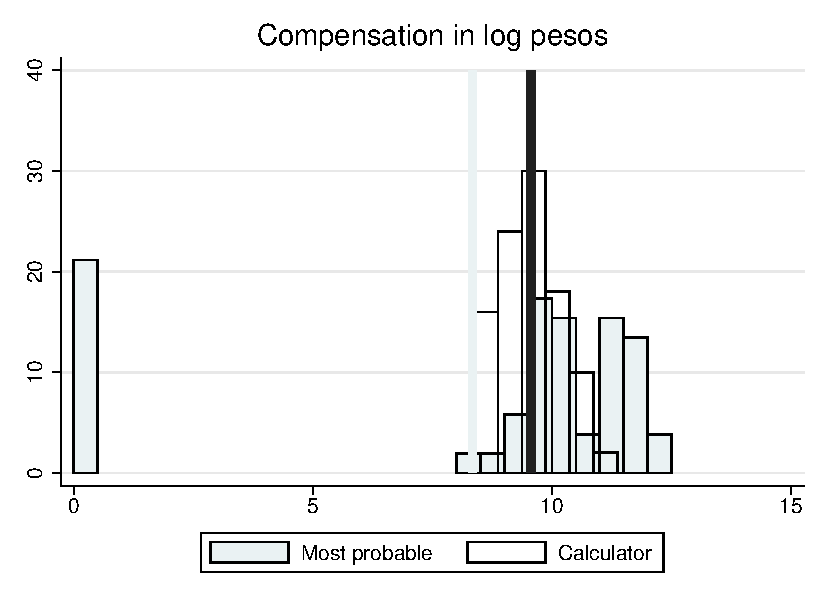
\includegraphics[width=\textwidth]{Compensation_comparison_employee.pdf}
    \end{subfigure}
     \begin{subfigure}{0.49\textwidth}
        \centering
        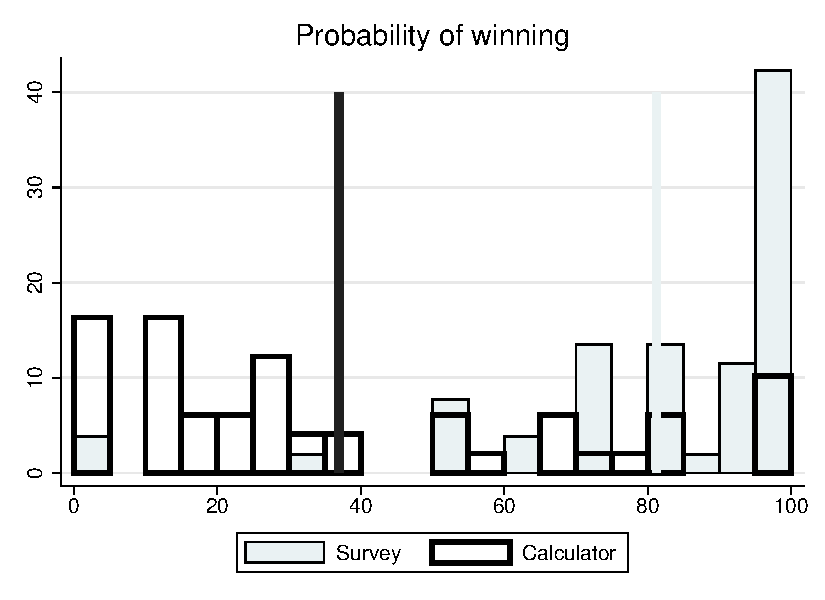
\includegraphics[width=\textwidth]{Probability_comparison_employee.pdf}
    \end{subfigure}
    \begin{subfigure}{0.49\textwidth}
        \caption{Employee Lawyer}
        \centering
        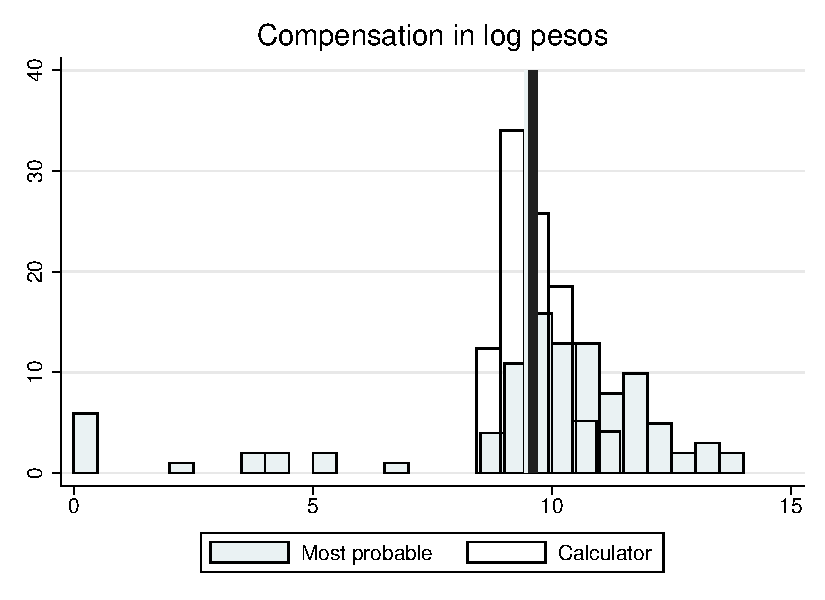
\includegraphics[width=\textwidth]{Compensation_comparison_EmployeeLawyer.pdf}
        \end{subfigure}
          \begin{subfigure}{0.49\textwidth}
        \centering
        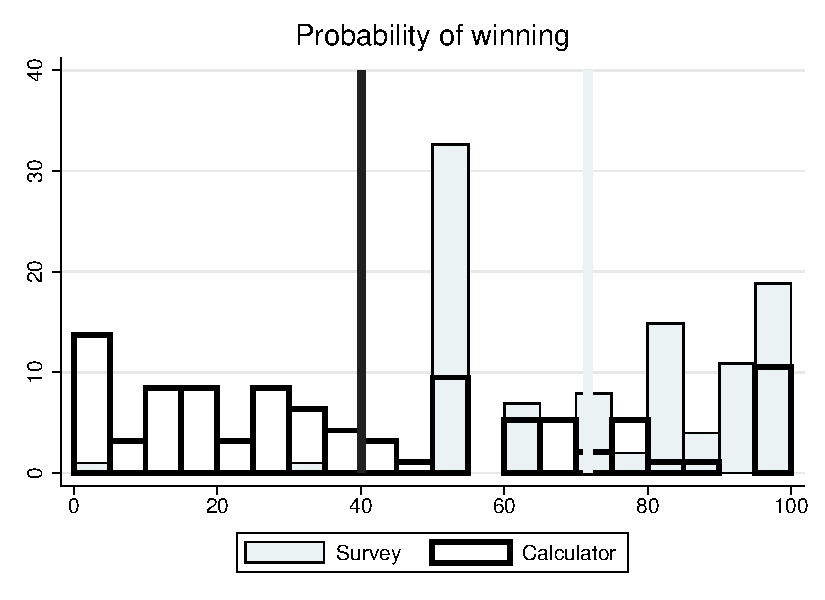
\includegraphics[width=\textwidth]{Probability_comparison_EmployeeLawyer.pdf}
    \end{subfigure}
        \begin{subfigure}{0.49\textwidth}
            \caption{Firm Lawyer}
            \centering
            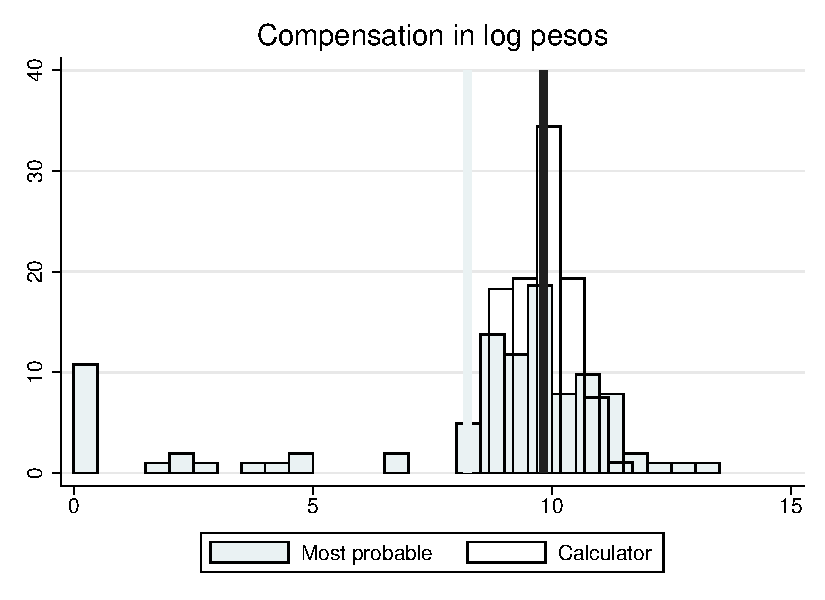
\includegraphics[width=\textwidth]{Compensation_comparison_FirmLawyer.pdf}
    \end{subfigure}
    \begin{subfigure}{0.49\textwidth}
            \centering
            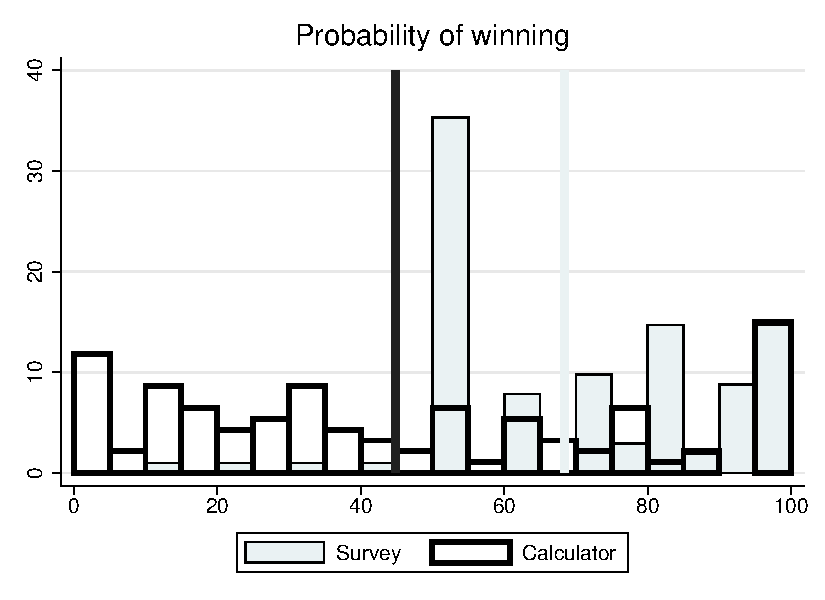
\includegraphics[width=\textwidth]{Probability_comparison_FirmLawyer.pdf}
        \end{subfigure}
    \end{center}
     \footnotesize \textit{Notes: Sample distributions for parties' expectations and calculator predictions.} Bandwidth for amount: 0.5 (log) pesos  Bandwidth for probability: 5\%. 
      \footnotesize{ \textit{Do file: }  \texttt{oc\_comparison.do}}
\end{figure}





\begin{figure}[H]
    \caption{Histograms of relative OC}
    \label{hist_rel_oc}
    \begin{center}
        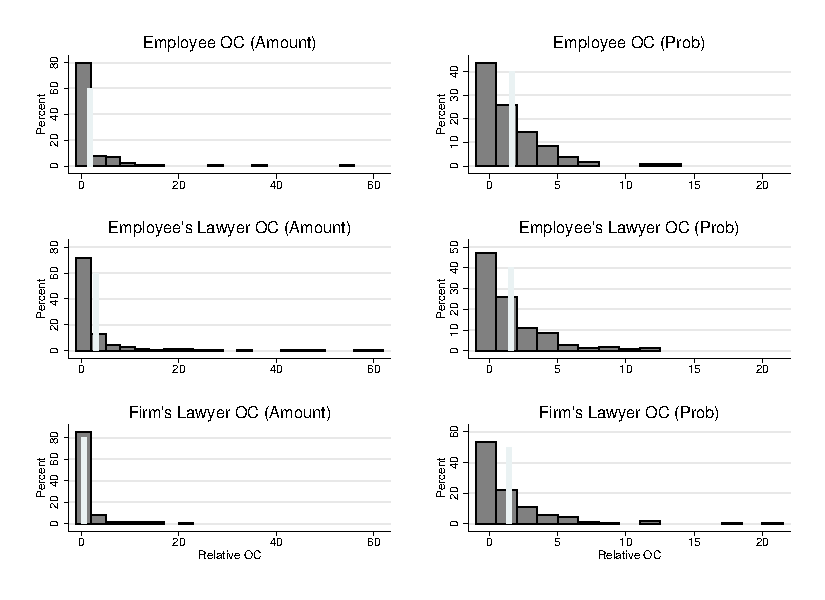
\includegraphics[width=0.9\textwidth]{hist_rel_oc.pdf}
        \end{center}
        {\footnotesize \textit{Notes: Histograms of relative overconfidence in amount an d probability. Relative overconfidence is measured as $\frac{survey-calc}{calc}$. The histograms only display up to the 98 percentile.}}
        \texttt{hist\_rel\_oc.do}
\end{figure}

      
\begin{figure}[H]
\caption{Number of experimental cases: overall, selected and actually treated.}
\label{treatmentunits}
\begin{center}
    \begin{subfigure}{0.49\textwidth}
        \caption{}
        \centering
        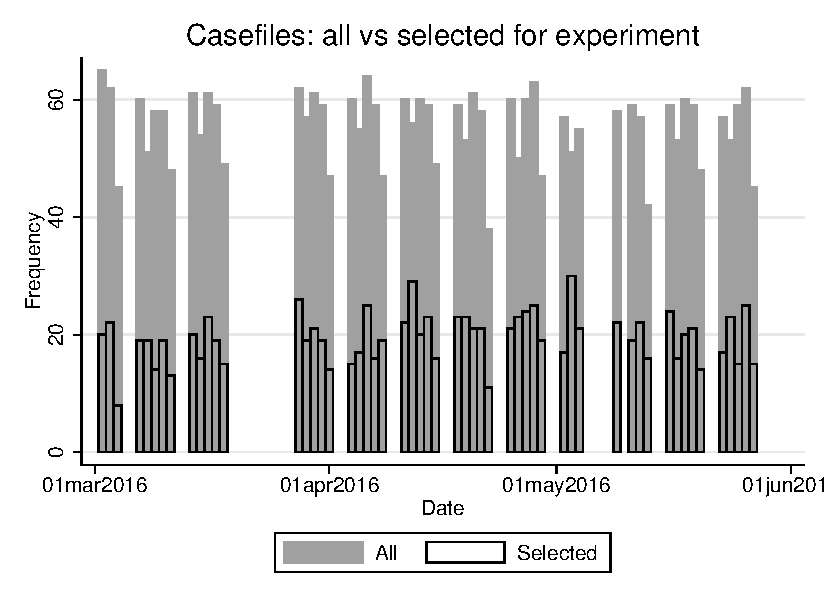
\includegraphics[width=\textwidth]{All_Selected.pdf}
    \end{subfigure}
    \begin{subfigure}{0.49\textwidth}
        \caption{}
        \centering
        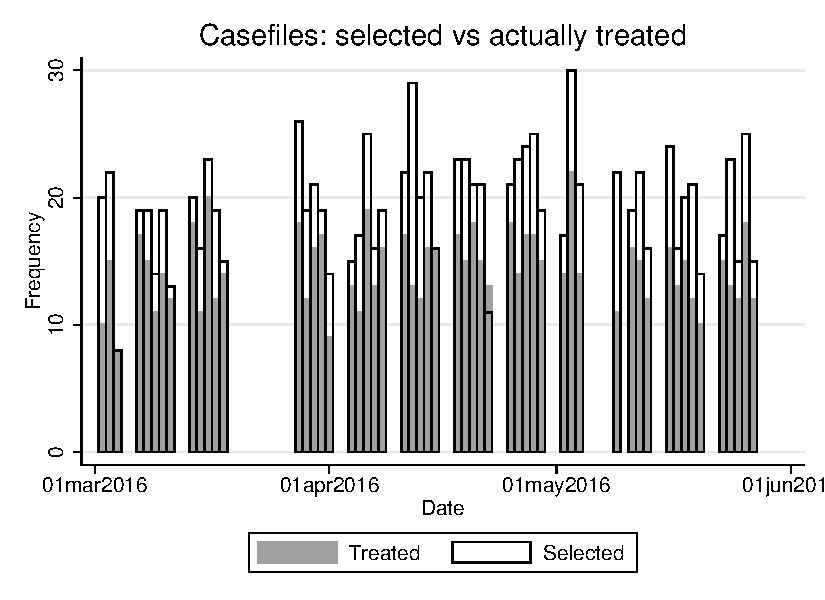
\includegraphics[width=\textwidth]{Selected_ActuallyT.pdf}
    \end{subfigure}
    \hfill
        \begin{subfigure}{0.49\textwidth}
            \caption{}
            \centering
            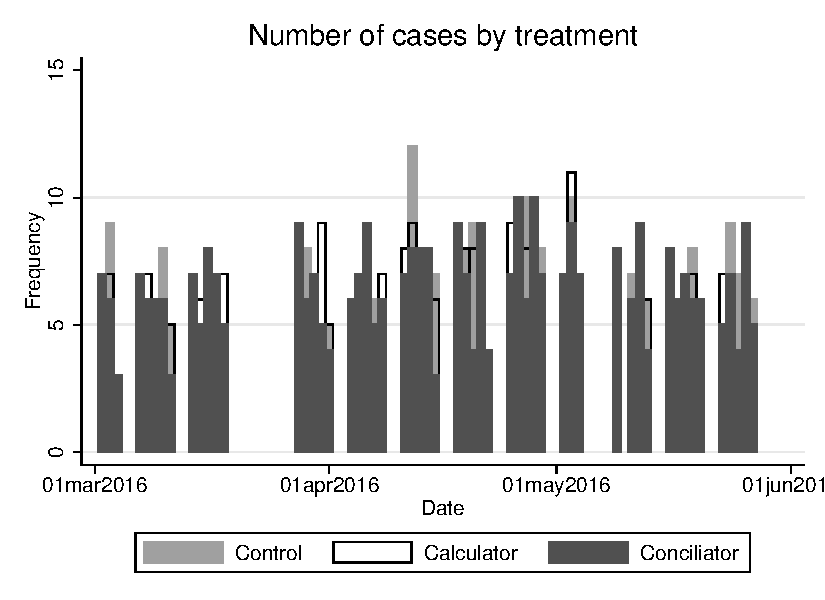
\includegraphics[width=\textwidth]{ByTreatment.pdf}    
        \end{subfigure}
    \end{center}
     {\footnotesize \textit{Notes: } Notes 
    The court we are working on is managing about 60 suits per day. Different suits are in different stages of the process (i.e. not all are new suits). Among the eligible ones we are selecting for treatment about 25 approximately. Among these we randomly select some for treatment and controls each day in equal proportions (except for indivisibilities of course). We have one control group that stays with the status quo, a calculator treatment that receives statistical information about the historical outcomes of cases similar to theirs, and a conciliator group that instead of getting statistical information talks with a court conciliator that explains (more on emotive grounds and some personal experience) why settling out of court may sometimes be better.}
      {\footnotesize \textit{Do file: }  \texttt{peiper6.do}}
\end{figure}


\begin{figure}[H]
    \label{figure_fotos}
    \caption{Implementation}
    \begin{center}
    \begin{subfigure}{0.4\textwidth}
        \caption{Survey area}
        \centering
        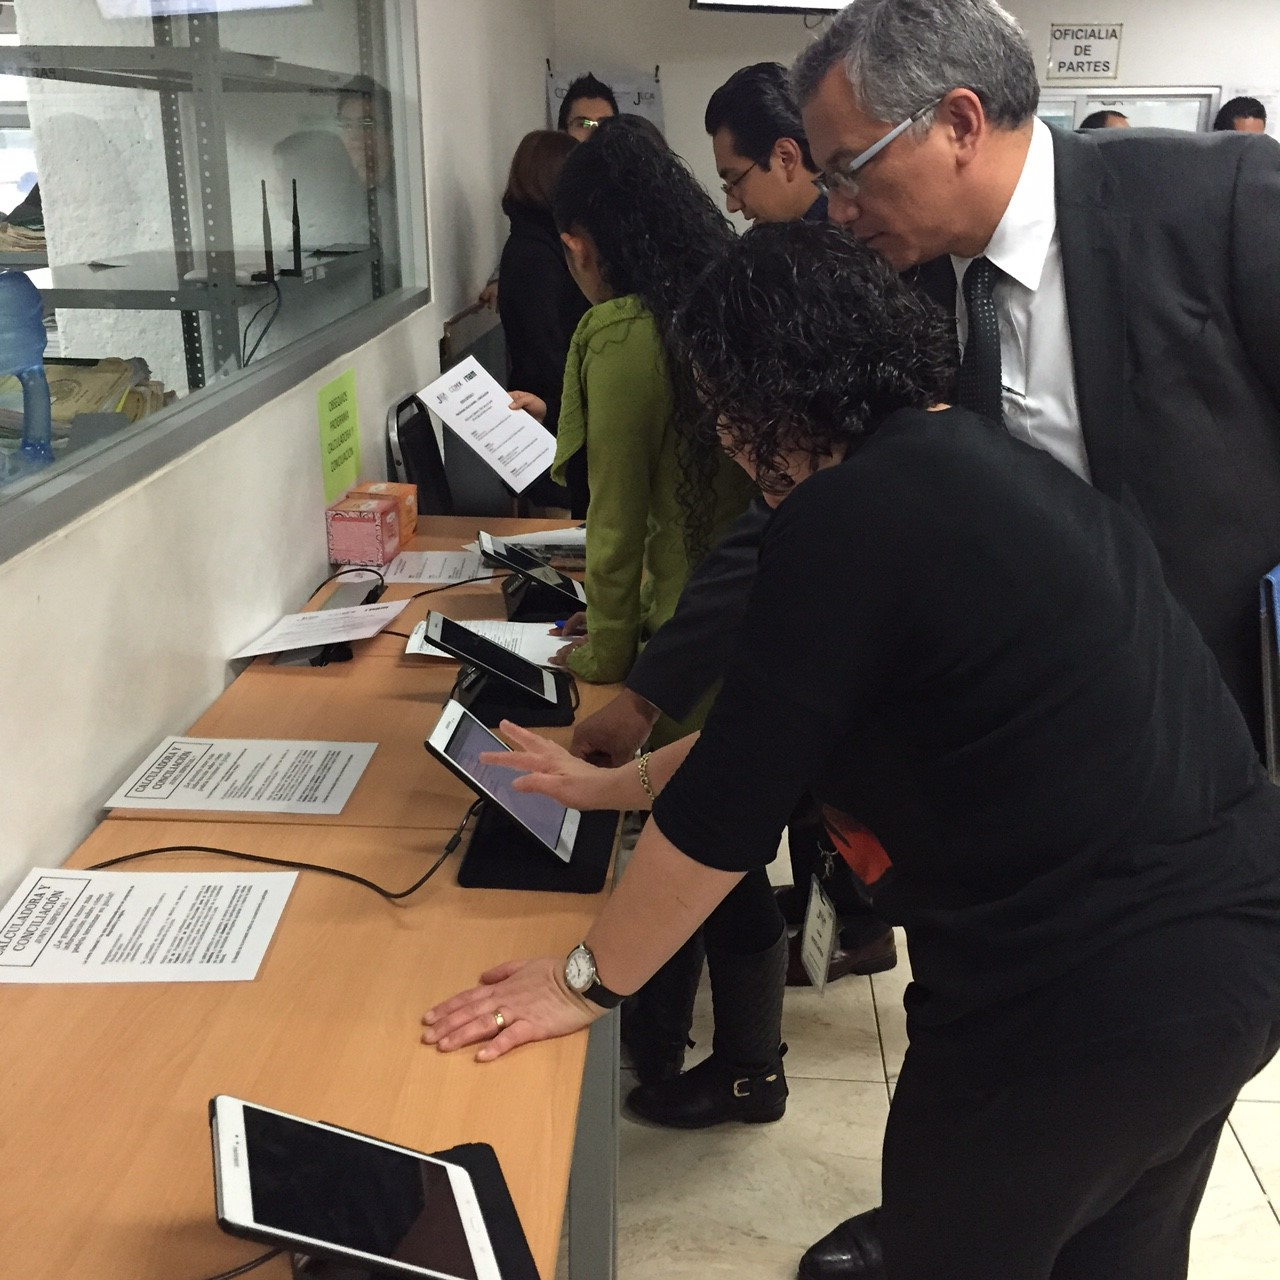
\includegraphics[width=\textwidth]{surveyarea.jpg}
    \end{subfigure}
    \begin{subfigure}{0.4\textwidth}
        \caption{Calculator treatment area}
        \centering
        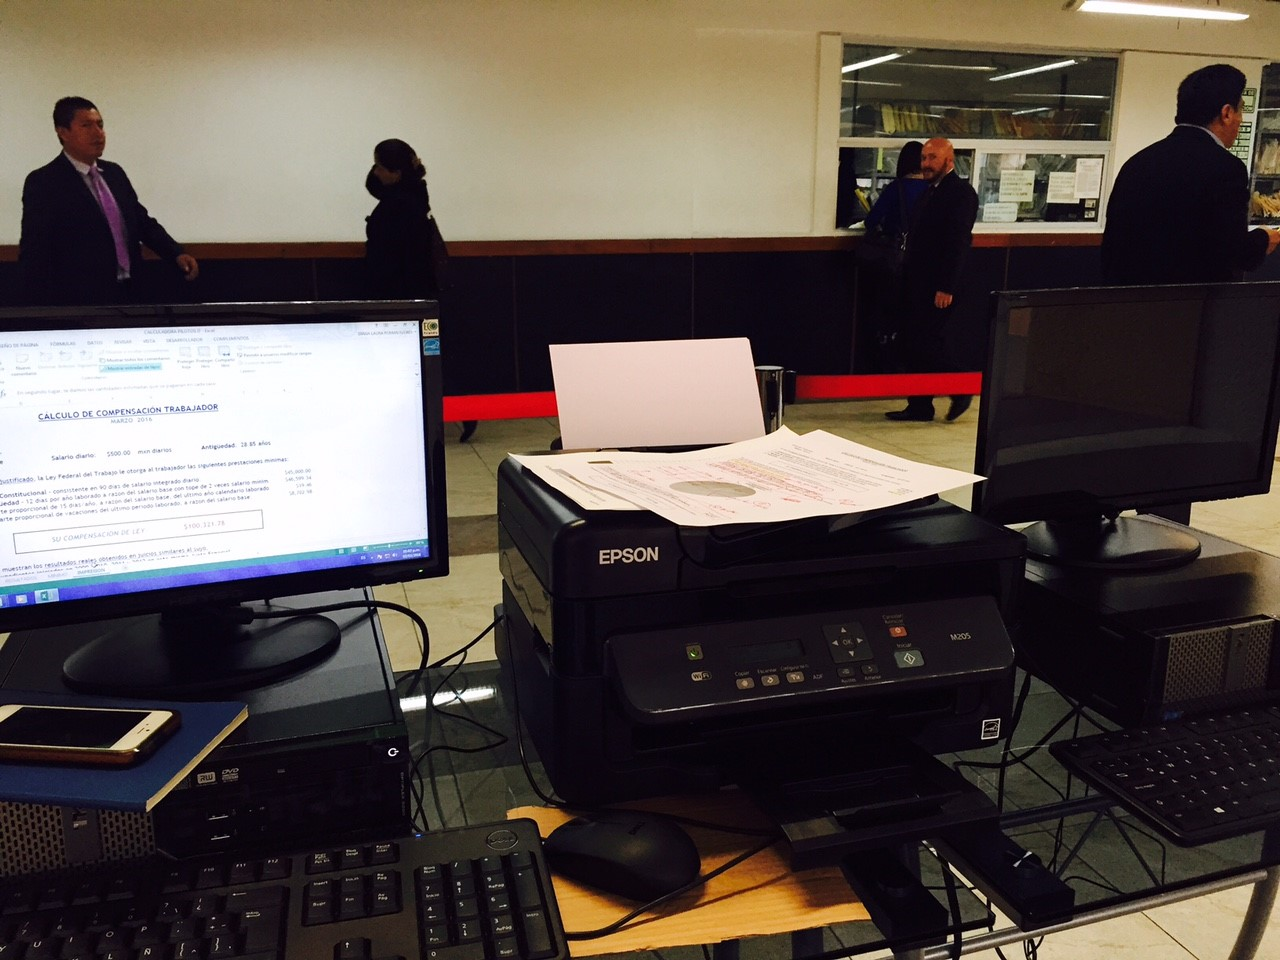
\includegraphics[width=\textwidth]{calcarea.jpg}
    \end{subfigure}
    \hfill
       \begin{subfigure}{0.4\textwidth}
        \caption{Conciliator's area}
        \centering
        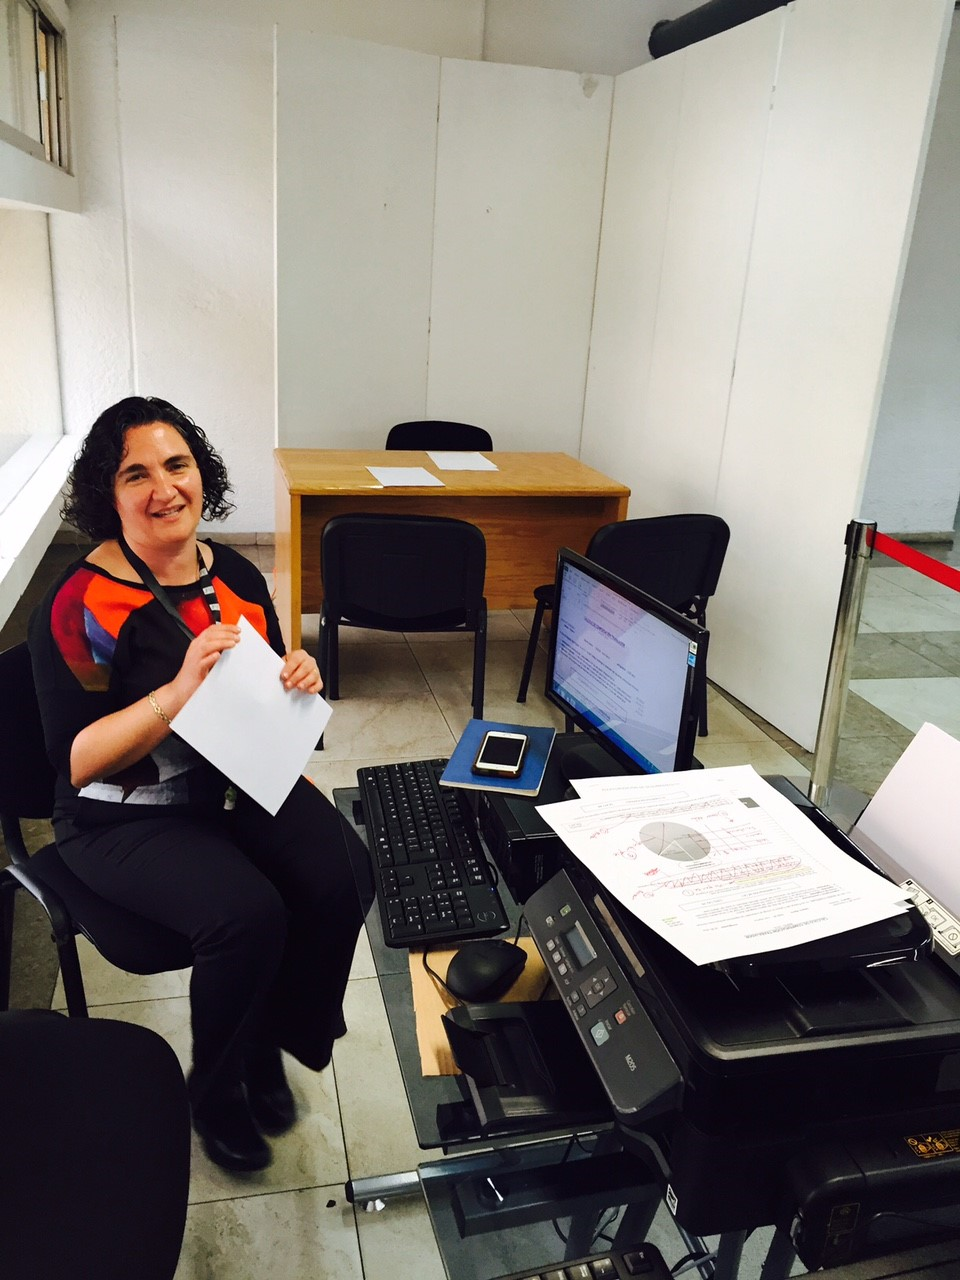
\includegraphics[width=\textwidth]{conciliatorarea.jpg}
    \end{subfigure}
    \begin{subfigure}{0.4\textwidth}
        \caption{Hearings in our court in a given day}
        \centering
        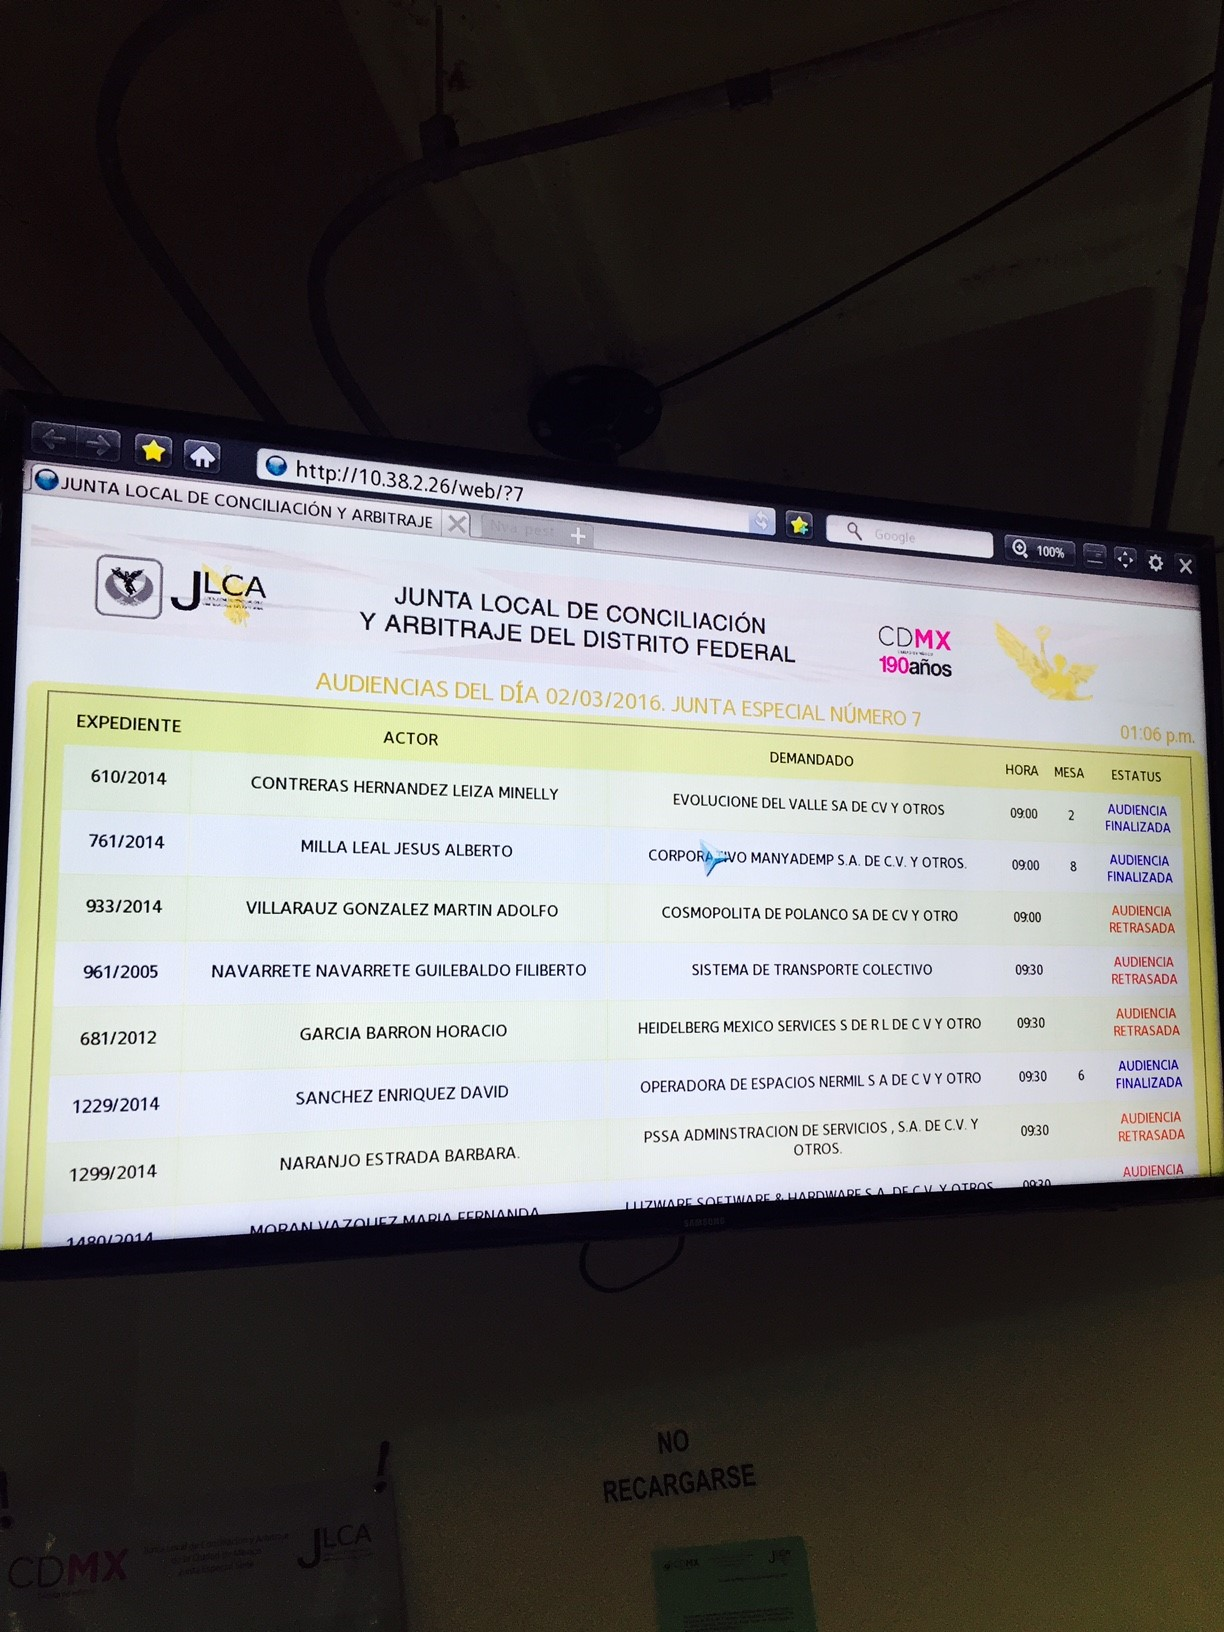
\includegraphics[width=\textwidth]{hearing.jpg}
    \end{subfigure} 
    
    \vspace{5mm}
    
     \footnotesize \textit{Notes: A little sample of the environment this experiment was conducted in. The survey area was just in front the counters in which hearings take place.}  
    \end{center}
\end{figure}




	
\pagebreak


\begin{figure}[H]
    \caption{Out of sample fit for duration predictions}
    \label{duration_predictions}
    \begin{center}
    \begin{subfigure}{0.49\textwidth}
    \centering
        \includegraphics[width=.75\textwidth]{mod_duracion_caducidad.tiff}
     \end{subfigure}
     \begin{subfigure}{0.49\textwidth}
    \centering
        \includegraphics[width=.75\textwidth]{mod_duracion_convenio.tiff}
     \end{subfigure}
     \hfill
         \begin{subfigure}{0.49\textwidth}
    \centering
        \includegraphics[width=.75\textwidth]{mod_duracion_laudo_pierde.tiff}
     \end{subfigure}
     \begin{subfigure}{0.49\textwidth}
    \centering
        \includegraphics[width=.75\textwidth]{mod_duracion_laudo_gana.tiff}
     \end{subfigure}
     \hfill
         \begin{subfigure}{0.49\textwidth}
    \centering
        \includegraphics[width=.75\textwidth]{mod_duracion_desiste.tiff}
     \end{subfigure}
        \end{center}
        {\footnotesize \textit{Notes: } Scatter plot of duration predictions and outcomes }
        {\footnotesize \textit{RScript: }  \texttt{covariate_plots.R}}
\end{figure}


\begin{figure}[H]
    \caption{Out of sample fit for compensation predictions}
    \label{}
    \begin{center}
    \begin{subfigure}{0.49\textwidth}
    \centering
        \includegraphics[width=.75\textwidth]{mod_liqtotal_convenio.tiff}
     \end{subfigure}
     \begin{subfigure}{0.49\textwidth}
    \centering
        \includegraphics[width=.75\textwidth]{mod_liqtotal_laudo_gana.tiff}
     \end{subfigure}
  \end{center}
        {\footnotesize \textit{Notes: } Scatter plot of compensation predictions and outcomes.}
        {\footnotesize \textit{RScript: }  \texttt{covariate_plots.R}}
\end{figure}

%\subsection{Model}
%
\subsection*{A Simple Game with Incomplete Information: Types and Beliefs}

\begin{dfn}[Game with incomplete information] A game with incomplete information $\mathcal{G}=(\Theta, S, P, u)$ consists of:
\begin{enumerate}[(i)]
\item A set $\Theta=\prod_{i\in I}\Theta_i$, where $\Theta_i$ is the finite set of possible types of player $i$ 
\item A set $S=\prod_{i\in I} S_i$, where $S_i$ is the set of possible strategies for player $i$
\item A joint probability distribution $p(\theta_1,\ldots, \theta_I)$ over types. For finite type space, we assume that $p(\theta_i)>0$ for all $\theta_i\in \Theta_i$
\item Payoff function $u_i:S\times \Theta\longmapsto \mathbb{R}$
\end{enumerate}
\end{dfn}

To study this type of games we rely on the idea by Harsanyi, assuming that the game begins with a move by nature which selects the different players’ preferences — or more generally, their types. So that the game can be thought as a \emph{complete} game but with \emph{imperfect information}
The type profile determines not only players’ payoffs but also their beliefs about other players’ types. Not everyone observes nature's move (player $i$ learns $\Theta_i$ but not $\Theta_{-i}$).\\

To analyze a game of incomplete information, we look at the \emph{Nash equilibrium} of the game where nature is a player. \\

A Bayesian pure strategy for player $i$ in $\mathcal{G}$ is a function from the possible set of types of player $i$ to the set of possible strategies.\\


\begin{dfn}[Bayesian-Nash equilibrium] A Bayesian strategy profile $(f_1,\ldots, f_I)$is a Bayesian-Nash equilibrium if for all $i$
\[f_i\in \text{argmax}_{f_{i}^{\prime}\in S_{i}^{\Theta_i}} \sum_{\theta\in \Theta} u_i\left(f_{i}^{\prime}(\theta_i), f_{-i}(\theta_{-i}),\theta_i, \theta_{-i}\right)p(\theta_i,\theta_{-i})\]
or alternatively, for all $i$, $\theta_i$ and $s_i$:
\[\sum_{\theta_{-i}\in \Theta_{-i}} u_i\left(f_{i}(\theta_i), f_{-i}(\theta_{-i}),\theta_i, \theta_{-i} \right) p(\theta_i|\theta_{-i})\geq \sum_{\theta_{-i}\in \Theta_{-i}} u_i\left(s_i, f_{-i}(\theta_{-i}),\theta_i, \theta_{-i} \right) p(\theta_i|\theta_{-i})\]
\end{dfn}

The second part of the definition just says that in order to maximize your expected payoff given that you know your types, then the strategy you choose for each type should maximize your payoff conditional on your having that type. Note that a Bayesian-Nash equilibrium is simply a Nash equilibrium in which nature moves first, chooses $\theta\in \Theta$ from a distribution with probability $p(\theta)$ and reveals $\theta_i$ to player $i$.\\

In the model introduced here, the source of uncertainty comes  as uncertainty about the types of players which translates as uncertainty in preferences and payoffs (the employee's lawyer (A)  and the employee (E) ) There can be 2 types of lawyers (Truthful and non-truthful) and 2 types of cases(High value and low value), which gives 4 settings. Payoffs are only known to the lawyer once he knows his type and the type of case. But because the players’ types are random and unknown to each other, they are uncertain about “who” their opponent is. However, they have the same beliefs about frequencies of opponent types.\\

Nature makes first move, choosing both the type of lawyer and type of case, the only one that knows this information is the lawyer. Once he knows his own type and the type of case, he sends a signal about the nature of the case (High value (H) / Low value (L) ) to the employee, and the latter makes the decision to sue (D) or not (N). \\

The 4 settings can be described as follows 

  \begin{table}[H]
  \begin{center}
    \setlength{\extrarowheight}{2pt}
    \begin{tabular}{*{4}{c|}}
      \multicolumn{2}{c}{} & \multicolumn{2}{c}{Player $E$}\\\cline{3-4}
      \multicolumn{1}{c}{} &  & $D$  & $ND$ \\\cline{2-4}
      \multirow{2}*{Player $A$}  & $H$ & $(1,x_1)$ & $(0,y_1)$ \\\cline{2-4}
      & $L$ & $(0,x_1)$ & $(0,y_1)$ \\\cline{2-4}
    \end{tabular}
            \begin{tabular}{*{4}{c|}}
      \multicolumn{2}{c}{} & \multicolumn{2}{c}{Player $E$}\\\cline{3-4}
      \multicolumn{1}{c}{} &  & $D$  & $ND$ \\\cline{2-4}
      \multirow{2}*{}  & $H$ & $(0,x_2)$ & $(0,y_2)$ \\\cline{2-4}
      & $L$ & $(0,x_2)$ & $(1,y_2)$ \\\cline{2-4}
    \end{tabular}
    \end{center}
  \end{table}
  
    \begin{table}[H]
      \begin{center}
    \setlength{\extrarowheight}{2pt}
        \begin{tabular}{*{4}{c|}}
      \multicolumn{2}{c}{} & \multicolumn{2}{c}{Player $E$}\\\cline{3-4}
      \multicolumn{1}{c}{} &  & $D$  & $ND$ \\\cline{2-4}
      \multirow{2}*{Player $A$}  & $H$ & $(1,x_3)$ & $(0,y_3)$ \\\cline{2-4}
      & $L$ & $(1,x_3)$ & $(0,y_3)$ \\\cline{2-4}
    \end{tabular}
        \begin{tabular}{*{4}{c|}}
      \multicolumn{2}{c}{} & \multicolumn{2}{c}{Player $E$}\\\cline{3-4}
      \multicolumn{1}{c}{} &  & $D$  & $ND$ \\\cline{2-4}
      \multirow{2}*{}  & $H$ & $(1,x_4)$ & $(0,y_4)$ \\\cline{2-4}
      & $L$ & $(1,x_4)$ & $(0,y_4)$ \\\cline{2-4}
    \end{tabular}
        \end{center}
   \footnotesize
    \textit{The 4 settings are respectively: Truthful-High value; Truthful-Low value; Non truthful-High value; Non truthful-Low value}         
  \end{table}

The rationale for the payoffs to be that way is intuitive. Consider the first game in which we have a truthful lawyer and a high value case, observe that lawyer has as dominant strategy to play $H$ and employee will be better off if he plays $D$ (sues), so that we impose the condition $x_1>y_1$. Note that $(H, D)$ corresponds to a Nash equilibrium, which is a desirable feature. In a similar fashion for the other 3 games we find that $x_2<y_2$, $x_3>y_3$ and $x_4<y_4$.\\

As the employee doesn't know in which of the 4 subgames she's actually in, the game can be described in extensive form as:
  
  
  
\begin{center}
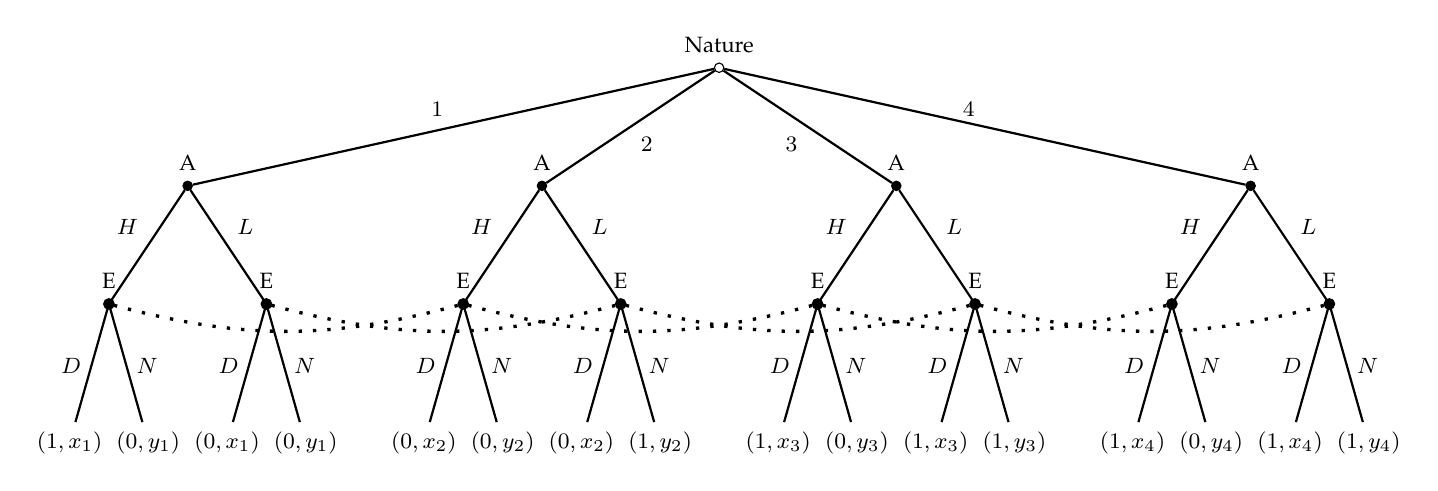
\begin{tikzpicture}[font=\footnotesize,edge from parent/.style={draw,thick}]
\label{geim}
% Two node styles: solid and hollow
\tikzstyle{solid node}=[circle,draw,inner sep=1.2,fill=black];
\tikzstyle{hollow node}=[circle,draw,inner sep=1.2];
% Specify spacing for each level of the tree
\tikzstyle{level 1}=[level distance=15mm,sibling distance=45mm]
\tikzstyle{level 2}=[level distance=15mm,sibling distance=20mm]
\tikzstyle{level 3}=[level distance=15mm,sibling distance=10mm]
% The Tree
\node(0)[hollow node ,label=above:{Nature}]{}
child{node[solid node,label=above:{A}]{}
child{node[solid node,label=above:{E}]{}
child{node[below]{$(1, x_1)$} edge from parent node[left]{$D$}}
child{node[below]{$(0,y_1)$} edge from parent node[right]{$N$}}
edge from parent node[above left]{$H$}
}
child{node[solid node,label=above:{E}]{}
child{node[below]{$(0,x_1)$} edge from parent node(s)[left]{$D$}}
child{node[below]{$(0,y_1)$} edge from parent node(N)[right]{$N$}}
edge from parent node[above right]{$L$}
}
edge from parent node[above left]{$1$}
}
child{node[solid node,label=above:{A}]{}
child{node[solid node,label=above:{E}]{}
child{node[below]{$(0,x_2)$} edge from parent node(m)[left]{$D$}}
child{node[below]{$(0,y_2)$} edge from parent node(n)[right]{$N$}}
edge from parent node[above left]{$H$}
}
child{node[solid node,label=above:{E}]{}
child{node[below]{$(0,x_2)$} edge from parent node[left]{$D$}}
child{node[below]{$(1,y_2)$} edge from parent node[right]{$N$}}
edge from parent node[above right]{$L$}
}
edge from parent node[below right]{$2$}
}
child{node[solid node,label=above:{A}]{}
child{node[solid node,label=above:{E}]{}
child{node[below]{$(1,x_3)$} edge from parent node[left]{$D$}}
child{node[below]{$(0,y_3)$} edge from parent node[right]{$N$}}
edge from parent node[above left]{$H$}
}
child{node[solid node,label=above:{E}]{}
child{node[below]{$(1,x_3)$} edge from parent node(D)[left]{$D$}}
child{node[below]{$(1,y_3)$} edge from parent node(N)[right]{$N$}}
edge from parent node[above right]{$L$}
}
edge from parent node[below left]{$3$}
}
child{node[solid node,label=above:{A}]{}
child{node[solid node,label=above:{E}]{}
child{node[below]{$(1,x_4)$} edge from parent node[left]{$D$}}
child{node[below]{$(0,y_4)$} edge from parent node[right]{$N$}}
edge from parent node[above left]{$H$}
}
child{node[solid node,label=above:{E}]{}
child{node[below]{$(1,x_4)$} edge from parent node(D)[left]{$D$}}
child{node[below]{$(1,y_4)$} edge from parent node(N)[right]{$N$}}
edge from parent node[above right]{$L$}
}
edge from parent node[above left]{$4$}
};
% information sets
\draw[loosely dotted,very thick](0-1-1)to[out=-15,in=195](0-2-1);
\draw[loosely dotted,very thick](0-1-2)to[out=-15,in=195](0-2-2);
\draw[loosely dotted,very thick](0-2-1)to[out=-15,in=195](0-3-1);
\draw[loosely dotted,very thick](0-2-2)to[out=-15,in=195](0-3-2);
\draw[loosely dotted,very thick](0-3-1)to[out=-15,in=195](0-4-1);
\draw[loosely dotted,very thick](0-3-2)to[out=-15,in=195](0-4-2);
% movers

\end{tikzpicture}
\end{center}


From the extensive form game we can deduce the payoffs to the 4 settings according to nature's choice. This is represented in the following tables:

\begin{table}[H]
\centering
\setlength\tabcolsep{4pt}
\begin{minipage}{0.48\textwidth}
\centering
        {% Table generated by Excel2LaTeX from sheet 'Hoja1'
\begin{tabular}{lrrrr}
\toprule
      & \multicolumn{1}{c}{DD} & \multicolumn{1}{c}{DN} & \multicolumn{1}{c}{ND} & \multicolumn{1}{c}{NN} \\
\midrule
HHHH  & \multicolumn{1}{l}{$( 1 , x_1 )$} & \multicolumn{1}{l}{$( 1 , x_1 )$} & \multicolumn{1}{l}{$( 0 , y_1 )$} & \multicolumn{1}{l}{$( 0 , y_1 )$} \\
HLHH  & \multicolumn{1}{l}{$( 1 , x_1 )$} & \multicolumn{1}{l}{$( 1 , x_1 )$} & \multicolumn{1}{l}{$( 0 , y_1 )$} & \multicolumn{1}{l}{$( 0 , y_1 )$} \\
HHLH  & \multicolumn{1}{l}{$( 1 , x_1 )$} & \multicolumn{1}{l}{$( 1 , x_1 )$} & \multicolumn{1}{l}{$( 0 , y_1 )$} & \multicolumn{1}{l}{$( 0 , y_1 )$} \\
HHHL  & \multicolumn{1}{l}{$( 1 , x_1 )$} & \multicolumn{1}{l}{$( 1 , x_1 )$} & \multicolumn{1}{l}{$( 0 , y_1 )$} & \multicolumn{1}{l}{$( 0 , y_1 )$} \\
HLLH  & \multicolumn{1}{l}{$( 1 , x_1 )$} & \multicolumn{1}{l}{$( 1 , x_1 )$} & \multicolumn{1}{l}{$( 0 , y_1 )$} & \multicolumn{1}{l}{$( 0 , y_1 )$} \\
HHLL  & \multicolumn{1}{l}{$( 1 , x_1 )$} & \multicolumn{1}{l}{$( 1 , x_1 )$} & \multicolumn{1}{l}{$( 0 , y_1 )$} & \multicolumn{1}{l}{$( 0 , y_1 )$} \\
HLHL  & \multicolumn{1}{l}{$( 1 , x_1 )$} & \multicolumn{1}{l}{$( 1 , x_1 )$} & \multicolumn{1}{l}{$( 0 , y_1 )$} & \multicolumn{1}{l}{$( 0 , y_1 )$} \\
HLLL  & \multicolumn{1}{l}{$( 1 , x_1 )$} & \multicolumn{1}{l}{$( 1 , x_1 )$} & \multicolumn{1}{l}{$( 0 , y_1 )$} & \multicolumn{1}{l}{$( 0 , y_1 )$} \\
LHHH  & \multicolumn{1}{l}{$( 0 , x_1 )$} & \multicolumn{1}{l}{$( 0 , y_1 )$} & \multicolumn{1}{l}{$( 0 , x_1 )$} & \multicolumn{1}{l}{$( 0 , y_1 )$} \\
LLHH  & \multicolumn{1}{l}{$( 0 , x_1 )$} & \multicolumn{1}{l}{$( 0 , y_1 )$} & \multicolumn{1}{l}{$( 0 , x_1 )$} & \multicolumn{1}{l}{$( 0 , y_1 )$} \\
LHLH  & \multicolumn{1}{l}{$( 0 , x_1 )$} & \multicolumn{1}{l}{$( 0 , y_1 )$} & \multicolumn{1}{l}{$( 0 , x_1 )$} & \multicolumn{1}{l}{$( 0 , y_1 )$} \\
LHHL  & \multicolumn{1}{l}{$( 0 , x_1 )$} & \multicolumn{1}{l}{$( 0 , y_1 )$} & \multicolumn{1}{l}{$( 0 , x_1 )$} & \multicolumn{1}{l}{$( 0 , y_1 )$} \\
LLLH  & \multicolumn{1}{l}{$( 0 , x_1 )$} & \multicolumn{1}{l}{$( 0 , y_1 )$} & \multicolumn{1}{l}{$( 0 , x_1 )$} & \multicolumn{1}{l}{$( 0 , y_1 )$} \\
LLHL  & \multicolumn{1}{l}{$( 0 , x_1 )$} & \multicolumn{1}{l}{$( 0 , y_1 )$} & \multicolumn{1}{l}{$( 0 , x_1 )$} & \multicolumn{1}{l}{$( 0 , y_1 )$} \\
LHLL  & \multicolumn{1}{l}{$( 0 , x_1 )$} & \multicolumn{1}{l}{$( 0 , y_1 )$} & \multicolumn{1}{l}{$( 0 , x_1 )$} & \multicolumn{1}{l}{$( 0 , y_1 )$} \\
LLLL  & \multicolumn{1}{l}{$( 0 , x_1 )$} & \multicolumn{1}{l}{$( 0 , y_1 )$} & \multicolumn{1}{l}{$( 0 , x_1 )$} & \multicolumn{1}{l}{$( 0 , y_1 )$} \\
\bottomrule
\end{tabular}%
}
\caption*{Payoff Matrix: Truthful Lawyer and High value case}
\label{PM1} 
\end{minipage}%
\hfill
\begin{minipage}{0.48\textwidth}
\centering
        {% Table generated by Excel2LaTeX from sheet 'Hoja1'
\begin{tabular}{lrrrr}
\toprule
      & \multicolumn{1}{c}{DD} & \multicolumn{1}{c}{DN} & \multicolumn{1}{c}{ND} & \multicolumn{1}{c}{NN} \\
\midrule
HHHH  & \multicolumn{1}{l}{$( 0 , x_2 )$} & \multicolumn{1}{l}{$( 0 , x_2 )$} & \multicolumn{1}{l}{$( 0 , y_2 )$} & \multicolumn{1}{l}{$( 0 , y_2 )$} \\
HLHH  & \multicolumn{1}{l}{$( 0 , x_2 )$} & \multicolumn{1}{l}{$( 1 , y_2 )$} & \multicolumn{1}{l}{$( 0 , x_2 )$} & \multicolumn{1}{l}{$( 1 , y_2 )$} \\
HHLH  & \multicolumn{1}{l}{$( 0 , x_2 )$} & \multicolumn{1}{l}{$( 0 , x_2 )$} & \multicolumn{1}{l}{$( 0 , y_2 )$} & \multicolumn{1}{l}{$( 0 , y_2 )$} \\
HHHL  & \multicolumn{1}{l}{$( 0 , x_2 )$} & \multicolumn{1}{l}{$( 0 , x_2 )$} & \multicolumn{1}{l}{$( 0 , y_2 )$} & \multicolumn{1}{l}{$( 0 , y_2 )$} \\
HLLH  & \multicolumn{1}{l}{$( 0 , x_2 )$} & \multicolumn{1}{l}{$( 1 , y_2 )$} & \multicolumn{1}{l}{$( 0 , x_2 )$} & \multicolumn{1}{l}{$( 1 , y_2 )$} \\
HHLL  & \multicolumn{1}{l}{$( 0 , x_2 )$} & \multicolumn{1}{l}{$( 0 , x_2 )$} & \multicolumn{1}{l}{$( 0 , y_2 )$} & \multicolumn{1}{l}{$( 0 , y_2 )$} \\
HLHL  & \multicolumn{1}{l}{$( 0 , x_2 )$} & \multicolumn{1}{l}{$( 1 , y_2 )$} & \multicolumn{1}{l}{$( 0 , x_2 )$} & \multicolumn{1}{l}{$( 1 , y_2 )$} \\
HLLL  & \multicolumn{1}{l}{$( 0 , x_2 )$} & \multicolumn{1}{l}{$( 1 , y_2 )$} & \multicolumn{1}{l}{$( 0 , x_2 )$} & \multicolumn{1}{l}{$( 1 , y_2 )$} \\
LHHH  & \multicolumn{1}{l}{$( 0 , x_2 )$} & \multicolumn{1}{l}{$( 0 , x_2 )$} & \multicolumn{1}{l}{$( 0 , y_2 )$} & \multicolumn{1}{l}{$( 0 , y_2 )$} \\
LLHH  & \multicolumn{1}{l}{$( 0 , x_2 )$} & \multicolumn{1}{l}{$( 1 , y_2 )$} & \multicolumn{1}{l}{$( 0 , x_2 )$} & \multicolumn{1}{l}{$( 1 , y_2 )$} \\
LHLH  & \multicolumn{1}{l}{$( 0 , x_2 )$} & \multicolumn{1}{l}{$( 0 , x_2 )$} & \multicolumn{1}{l}{$( 0 , y_2 )$} & \multicolumn{1}{l}{$( 0 , y_2 )$} \\
LHHL  & \multicolumn{1}{l}{$( 0 , x_2 )$} & \multicolumn{1}{l}{$( 0 , x_2 )$} & \multicolumn{1}{l}{$( 0 , y_2 )$} & \multicolumn{1}{l}{$( 0 , y_2 )$} \\
LLLH  & \multicolumn{1}{l}{$( 0 , x_2 )$} & \multicolumn{1}{l}{$( 1 , y_2 )$} & \multicolumn{1}{l}{$( 0 , x_2 )$} & \multicolumn{1}{l}{$( 1 , y_2 )$} \\
LLHL  & \multicolumn{1}{l}{$( 0 , x_2 )$} & \multicolumn{1}{l}{$( 1 , y_2 )$} & \multicolumn{1}{l}{$( 0 , x_2 )$} & \multicolumn{1}{l}{$( 1 , y_2 )$} \\
LHLL  & \multicolumn{1}{l}{$( 0 , x_2 )$} & \multicolumn{1}{l}{$( 0 , x_2 )$} & \multicolumn{1}{l}{$( 0 , y_2 )$} & \multicolumn{1}{l}{$( 0 , y_2 )$} \\
LLLL  & \multicolumn{1}{l}{$( 0 , x_2 )$} & \multicolumn{1}{l}{$( 1 , y_2 )$} & \multicolumn{1}{l}{$( 0 , x_2 )$} & \multicolumn{1}{l}{$( 1 , y_2 )$} \\
\bottomrule
\end{tabular}%
}
\caption*{Payoff Matrix: Truthful Lawyer and Low value case}
\label{PM2} 
\end{minipage}%
\end{table}


\begin{table}[H]
\centering
\setlength\tabcolsep{4pt}
\begin{minipage}{0.48\textwidth}
\centering
        {% Table generated by Excel2LaTeX from sheet 'Hoja1'
\begin{tabular}{lrrrr}
\toprule
      & \multicolumn{1}{c}{DD} & \multicolumn{1}{c}{DN} & \multicolumn{1}{c}{ND} & \multicolumn{1}{c}{NN} \\
\midrule
HHHH  & \multicolumn{1}{l}{$( 1 , x_3 )$} & \multicolumn{1}{l}{$( 1 , x_3 )$} & \multicolumn{1}{l}{$( 0 , y_3 )$} & \multicolumn{1}{l}{$( 0 , y_3 )$} \\
HLHH  & \multicolumn{1}{l}{$( 1 , x_3 )$} & \multicolumn{1}{l}{$( 1 , x_3 )$} & \multicolumn{1}{l}{$( 0 , y_3 )$} & \multicolumn{1}{l}{$( 0 , y_3 )$} \\
HHLH  & \multicolumn{1}{l}{$( 1 , x_3 )$} & \multicolumn{1}{l}{$( 0 , y_3 )$} & \multicolumn{1}{l}{$( 1 , x_3 )$} & \multicolumn{1}{l}{$( 0 , y_3 )$} \\
HHHL  & \multicolumn{1}{l}{$( 1 , x_3 )$} & \multicolumn{1}{l}{$( 1 , x_3 )$} & \multicolumn{1}{l}{$( 0 , y_3 )$} & \multicolumn{1}{l}{$( 0 , y_3 )$} \\
HLLH  & \multicolumn{1}{l}{$( 1 , x_3 )$} & \multicolumn{1}{l}{$( 0 , y_3 )$} & \multicolumn{1}{l}{$( 1 , x_3 )$} & \multicolumn{1}{l}{$( 0 , y_3 )$} \\
HHLL  & \multicolumn{1}{l}{$( 1 , x_3 )$} & \multicolumn{1}{l}{$( 0 , y_3 )$} & \multicolumn{1}{l}{$( 1 , x_3 )$} & \multicolumn{1}{l}{$( 0 , y_3 )$} \\
HLHL  & \multicolumn{1}{l}{$( 1 , x_3 )$} & \multicolumn{1}{l}{$( 1 , x_3 )$} & \multicolumn{1}{l}{$( 0 , y_3 )$} & \multicolumn{1}{l}{$( 0 , y_3 )$} \\
HLLL  & \multicolumn{1}{l}{$( 1 , x_3 )$} & \multicolumn{1}{l}{$( 0 , y_3 )$} & \multicolumn{1}{l}{$( 1 , x_3 )$} & \multicolumn{1}{l}{$( 0 , y_3 )$} \\
LHHH  & \multicolumn{1}{l}{$( 1 , x_3 )$} & \multicolumn{1}{l}{$( 1 , x_3 )$} & \multicolumn{1}{l}{$( 0 , y_3 )$} & \multicolumn{1}{l}{$( 0 , y_3 )$} \\
LLHH  & \multicolumn{1}{l}{$( 1 , x_3 )$} & \multicolumn{1}{l}{$( 1 , x_3 )$} & \multicolumn{1}{l}{$( 0 , y_3 )$} & \multicolumn{1}{l}{$( 0 , y_3 )$} \\
LHLH  & \multicolumn{1}{l}{$( 1 , x_3 )$} & \multicolumn{1}{l}{$( 0 , y_3 )$} & \multicolumn{1}{l}{$( 1 , x_3 )$} & \multicolumn{1}{l}{$( 0 , y_3 )$} \\
LHHL  & \multicolumn{1}{l}{$( 1 , x_3 )$} & \multicolumn{1}{l}{$( 1 , x_3 )$} & \multicolumn{1}{l}{$( 0 , y_3 )$} & \multicolumn{1}{l}{$( 0 , y_3 )$} \\
LLLH  & \multicolumn{1}{l}{$( 1 , x_3 )$} & \multicolumn{1}{l}{$( 0 , y_3 )$} & \multicolumn{1}{l}{$( 1 , x_3 )$} & \multicolumn{1}{l}{$( 0 , y_3 )$} \\
LLHL  & \multicolumn{1}{l}{$( 1 , x_3 )$} & \multicolumn{1}{l}{$( 1 , x_3 )$} & \multicolumn{1}{l}{$( 0 , y_3 )$} & \multicolumn{1}{l}{$( 0 , y_3 )$} \\
LHLL  & \multicolumn{1}{l}{$( 1 , x_3 )$} & \multicolumn{1}{l}{$( 0 , y_3 )$} & \multicolumn{1}{l}{$( 1 , x_3 )$} & \multicolumn{1}{l}{$( 0 , y_3 )$} \\
LLLL  & \multicolumn{1}{l}{$( 1 , x_3 )$} & \multicolumn{1}{l}{$( 0 , y_3 )$} & \multicolumn{1}{l}{$( 1 , x_3 )$} & \multicolumn{1}{l}{$( 0 , y_3 )$} \\
\bottomrule
\end{tabular}%
}
\caption*{Payoff Matrix: Non-truthful Lawyer and High value case}
\label{PM3} 
\end{minipage}%
\hfill
\begin{minipage}{0.48\textwidth}
\centering
        {% Table generated by Excel2LaTeX from sheet 'Hoja1'
\begin{tabular}{lrrrr}
\toprule
      & \multicolumn{1}{c}{DD} & \multicolumn{1}{c}{DN} & \multicolumn{1}{c}{ND} & \multicolumn{1}{c}{NN} \\
\midrule
HHHH  & \multicolumn{1}{l}{$( 1 , x_4 )$} & \multicolumn{1}{l}{$( 1 , x_4 )$} & \multicolumn{1}{l}{$( 0 , y_4 )$} & \multicolumn{1}{l}{$( 0 , y_4 )$} \\
HLHH  & \multicolumn{1}{l}{$( 1 , x_4 )$} & \multicolumn{1}{l}{$( 1 , x_4 )$} & \multicolumn{1}{l}{$( 0 , y_4 )$} & \multicolumn{1}{l}{$( 0 , y_4 )$} \\
HHLH  & \multicolumn{1}{l}{$( 1 , x_4 )$} & \multicolumn{1}{l}{$( 1 , x_4 )$} & \multicolumn{1}{l}{$( 0 , y_4 )$} & \multicolumn{1}{l}{$( 0 , y_4 )$} \\
HHHL  & \multicolumn{1}{l}{$( 1 , x_4 )$} & \multicolumn{1}{l}{$( 0 , y_4 )$} & \multicolumn{1}{l}{$( 1 , x_4 )$} & \multicolumn{1}{l}{$( 0 , y_4 )$} \\
HLLH  & \multicolumn{1}{l}{$( 1 , x_4 )$} & \multicolumn{1}{l}{$( 1 , x_4 )$} & \multicolumn{1}{l}{$( 0 , y_4 )$} & \multicolumn{1}{l}{$( 0 , y_4 )$} \\
HHLL  & \multicolumn{1}{l}{$( 1 , x_4 )$} & \multicolumn{1}{l}{$( 0 , y_4 )$} & \multicolumn{1}{l}{$( 1 , x_4 )$} & \multicolumn{1}{l}{$( 0 , y_4 )$} \\
HLHL  & \multicolumn{1}{l}{$( 1 , x_4 )$} & \multicolumn{1}{l}{$( 0 , y_4 )$} & \multicolumn{1}{l}{$( 1 , x_4 )$} & \multicolumn{1}{l}{$( 0 , y_4 )$} \\
HLLL  & \multicolumn{1}{l}{$( 1 , x_4 )$} & \multicolumn{1}{l}{$( 0 , y_4 )$} & \multicolumn{1}{l}{$( 1 , x_4 )$} & \multicolumn{1}{l}{$( 0 , y_4 )$} \\
LHHH  & \multicolumn{1}{l}{$( 1 , x_4 )$} & \multicolumn{1}{l}{$( 1 , x_4 )$} & \multicolumn{1}{l}{$( 0 , y_4 )$} & \multicolumn{1}{l}{$( 0 , y_4 )$} \\
LLHH  & \multicolumn{1}{l}{$( 1 , x_4 )$} & \multicolumn{1}{l}{$( 1 , x_4 )$} & \multicolumn{1}{l}{$( 0 , y_4 )$} & \multicolumn{1}{l}{$( 0 , y_4 )$} \\
LHLH  & \multicolumn{1}{l}{$( 1 , x_4 )$} & \multicolumn{1}{l}{$( 1 , x_4 )$} & \multicolumn{1}{l}{$( 0 , y_4 )$} & \multicolumn{1}{l}{$( 0 , y_4 )$} \\
LHHL  & \multicolumn{1}{l}{$( 1 , x_4 )$} & \multicolumn{1}{l}{$( 0 , y_4 )$} & \multicolumn{1}{l}{$( 1 , x_4 )$} & \multicolumn{1}{l}{$( 0 , y_4 )$} \\
LLLH  & \multicolumn{1}{l}{$( 1 , x_4 )$} & \multicolumn{1}{l}{$( 1 , x_4 )$} & \multicolumn{1}{l}{$( 0 , y_4 )$} & \multicolumn{1}{l}{$( 0 , y_4 )$} \\
LLHL  & \multicolumn{1}{l}{$( 1 , x_4 )$} & \multicolumn{1}{l}{$( 0 , y_4 )$} & \multicolumn{1}{l}{$( 1 , x_4 )$} & \multicolumn{1}{l}{$( 0 , y_4 )$} \\
LHLL  & \multicolumn{1}{l}{$( 1 , x_4 )$} & \multicolumn{1}{l}{$( 0 , y_4 )$} & \multicolumn{1}{l}{$( 1 , x_4 )$} & \multicolumn{1}{l}{$( 0 , y_4 )$} \\
LLLL  & \multicolumn{1}{l}{$( 1 , x_4 )$} & \multicolumn{1}{l}{$( 0 , y_4 )$} & \multicolumn{1}{l}{$( 1 , x_4 )$} & \multicolumn{1}{l}{$( 0 , y_4 )$} \\
\bottomrule
\end{tabular}%
}
\caption*{Payoff Matrix: Non-truthful Lawyer and Low value case}
\label{PM4} 
\end{minipage}%
\end{table}

The actual payoff matrix is the weighted sum of each of the 4 settings, which gives

\begin{table}[H]
\centering
        {% Table generated by Excel2LaTeX from sheet 'Hoja1'
\begin{tabular}{rrr}
\toprule
\toprule
      & \multicolumn{1}{c}{\colorbox{red}{DD}} & \multicolumn{1}{c}{\colorbox{red}{DN}} \\
\midrule
\multicolumn{1}{l}{\colorbox{blue}{HHHH}} & \multicolumn{1}{l}{\colorbox{yellow}{$( p_1+p_3+p_4\;\; ,\;\; p_1x_1+p_2x_2+p_3x_3+p_4x_4 )$}} & \multicolumn{1}{l}{$( p_1+p_3+p_4\;\; ,\;\; p_1x_1+p_2x_2+p_3x_3+p_4x_4 )$} \\
\multicolumn{1}{l}{\colorbox{blue}{HLHH}} & \multicolumn{1}{l}{$( p_1+p_3+p_4\;\; ,\;\; p_1x_1+p_2x_2+p_3x_3+p_4x_4 )$} & \multicolumn{1}{l}{\colorbox{yellow}{$( p_1+p_2+p_3+p_4\;\; ,\;\; p_1x_1+p_2y_2+p_3x_3+p_4x_4 )$}} \\
\multicolumn{1}{l}{\colorbox{blue}{HHLH}} & \multicolumn{1}{l}{\colorbox{yellow}{$( p_1+p_3+p_4\;\; ,\;\; p_1x_1+p_2x_2+p_3x_3+p_4x_4 )$}} & \multicolumn{1}{l}{$( p_1+p_4\;\; ,\;\; p_1x_1+p_2x_2+p_3y_3+p_4x_4 )$} \\
\multicolumn{1}{l}{HHHL} & \multicolumn{1}{l}{$( p_1+p_3+p_4\;\; ,\;\; p_1x_1+p_2x_2+p_3x_3+p_4x_4 )$} & \multicolumn{1}{l}{$( p_1+p_3\;\; ,\;\; p_1x_1+p_2x_2+p_3x_3+p_4y_4 )$} \\
\multicolumn{1}{l}{\colorbox{blue}{HLLH}} & \multicolumn{1}{l}{\colorbox{yellow}{$( p_1+p_3+p_4\;\; ,\;\; p_1x_1+p_2x_2+p_3x_3+p_4x_4 )$}} & \multicolumn{1}{l}{$( p_1+p_2+p_4\;\; ,\;\; p_1x_1+p_2y_2+p_3y_3+p_4x_4 )$} \\
\multicolumn{1}{l}{HHLL} & \multicolumn{1}{l}{$( p_1+p_3+p_4\;\; ,\;\; p_1x_1+p_2x_2+p_3x_3+p_4x_4 )$} & \multicolumn{1}{l}{$( p_1\;\; ,\;\; p_1x_1+p_2x_2+p_3y_3+p_4y_4 )$} \\
\multicolumn{1}{l}{HLHL} & \multicolumn{1}{l}{$( p_1+p_3+p_4\;\; ,\;\; p_1x_1+p_2x_2+p_3x_3+p_4x_4 )$} & \multicolumn{1}{l}{$( p_1+p_2+p_3\;\; ,\;\; p_1x_1+p_2y_2+p_3x_3+p_4y_4 )$} \\
\multicolumn{1}{l}{HLLL} & \multicolumn{1}{l}{$( p_1+p_3+p_4\;\; ,\;\; p_1x_1+p_2x_2+p_3x_3+p_4x_4 )$} & \multicolumn{1}{l}{$( p_1+p_2\;\; ,\;\; p_1x_1+p_2y_2+p_3y_3+p_4y_4 )$} \\
\multicolumn{1}{l}{\colorbox{blue}{LHHH}} & \multicolumn{1}{l}{$( p_3+p_4\;\; ,\;\; p_1x_1+p_2x_2+p_3x_3+p_4x_4 )$} & \multicolumn{1}{l}{$( p_3+p_4\;\; ,\;\; p_1y_1+p_2x_2+p_3x_3+p_4x_4 )$} \\
\multicolumn{1}{l}{\colorbox{blue}{LLHH}} & \multicolumn{1}{l}{$( p_3+p_4\;\; ,\;\; p_1x_1+p_2x_2+p_3x_3+p_4x_4 )$} & \multicolumn{1}{l}{$( p_2+p_3+p_4\;\; ,\;\; p_1y_1+p_2y_2+p_3x_3+p_4x_4 )$} \\
\multicolumn{1}{l}{\colorbox{blue}{LHLH}} & \multicolumn{1}{l}{$( p_3+p_4\;\; ,\;\; p_1x_1+p_2x_2+p_3x_3+p_4x_4 )$} & \multicolumn{1}{l}{$( p_4\;\; ,\;\; p_1y_1+p_2x_2+p_3y_3+p_4x_4 )$} \\
\multicolumn{1}{l}{LHHL} & \multicolumn{1}{l}{$( p_3+p_4\;\; ,\;\; p_1x_1+p_2x_2+p_3x_3+p_4x_4 )$} & \multicolumn{1}{l}{$( p_3\;\; ,\;\; p_1y_1+p_2x_2+p_3x_3+p_4y_4 )$} \\
\multicolumn{1}{l}{\colorbox{blue}{LLLH}} & \multicolumn{1}{l}{$( p_3+p_4\;\; ,\;\; p_1x_1+p_2x_2+p_3x_3+p_4x_4 )$} & \multicolumn{1}{l}{$( p_2+p_4\;\; ,\;\; p_1y_1+p_2y_2+p_3y_3+p_4x_4 )$} \\
\multicolumn{1}{l}{LLHL} & \multicolumn{1}{l}{$( p_3+p_4\;\; ,\;\; p_1x_1+p_2x_2+p_3x_3+p_4x_4 )$} & \multicolumn{1}{l}{$( p_2+p_3\;\; ,\;\; p_1y_1+p_2y_2+p_3x_3+p_4y_4 )$} \\
\multicolumn{1}{l}{LHLL} & \multicolumn{1}{l}{$( p_3+p_4\;\; ,\;\; p_1x_1+p_2x_2+p_3x_3+p_4x_4 )$} & \multicolumn{1}{l}{$( 0\;\; ,\;\; p_1y_1+p_2x_2+p_3y_3+p_4y_4 )$} \\
\multicolumn{1}{l}{LLLL} & \multicolumn{1}{l}{$( p_3+p_4\;\; ,\;\; p_1x_1+p_2x_2+p_3x_3+p_4x_4 )$} & \multicolumn{1}{l}{$( p_2\;\; ,\;\; p_1y_1+p_2y_2+p_3y_3+p_4y_4 )$} \\
      &       &  \\
      \toprule
      \toprule
      & \multicolumn{1}{c}{ND} & \multicolumn{1}{c}{NN} \\
      \midrule
\multicolumn{1}{l}{HHHH} & \multicolumn{1}{l}{$( 0\;\; ,\;\; p_1y_1+p_2y_2+p_3y_3+p_4y_4 )$} & \multicolumn{1}{l}{$( 0\;\; ,\;\; p_1y_1+p_2y_2+p_3y_3+p_4y_4 )$} \\
\multicolumn{1}{l}{HLHH} & \multicolumn{1}{l}{$( 0\;\; ,\;\; p_1y_1+p_2x_2+p_3y_3+p_4y_4 )$} & \multicolumn{1}{l}{$( p_2\;\; ,\;\; p_1y_1+p_2y_2+p_3y_3+p_4y_4 )$} \\
\multicolumn{1}{l}{HHLH} & \multicolumn{1}{l}{$( p_3\;\; ,\;\; p_1y_1+p_2y_2+p_3x_3+p_4y_4 )$} & \multicolumn{1}{l}{$( 0\;\; ,\;\; p_1y_1+p_2y_2+p_3y_3+p_4y_4 )$} \\
\multicolumn{1}{l}{HHHL} & \multicolumn{1}{l}{$( p_4\;\; ,\;\; p_1y_1+p_2y_2+p_3y_3+p_4x_4 )$} & \multicolumn{1}{l}{$( 0\;\; ,\;\; p_1y_1+p_2y_2+p_3y_3+p_4y_4 )$} \\
\multicolumn{1}{l}{HLLH} & \multicolumn{1}{l}{$( p_3\;\; ,\;\; p_1y_1+p_2x_2+p_3x_3+p_4y_4 )$} & \multicolumn{1}{l}{$( p_2\;\; ,\;\; p_1y_1+p_2y_2+p_3y_3+p_4y_4 )$} \\
\multicolumn{1}{l}{HHLL} & \multicolumn{1}{l}{$( p_3+p_4\;\; ,\;\; p_1y_1+p_2y_2+p_3x_3+p_4x_4 )$} & \multicolumn{1}{l}{$( 0\;\; ,\;\; p_1y_1+p_2y_2+p_3y_3+p_4y_4 )$} \\
\multicolumn{1}{l}{HLHL} & \multicolumn{1}{l}{$( p_4\;\; ,\;\; p_1y_1+p_2x_2+p_3y_3+p_4x_4 )$} & \multicolumn{1}{l}{$( p_2\;\; ,\;\; p_1y_1+p_2y_2+p_3y_3+p_4y_4 )$} \\
\multicolumn{1}{l}{HLLL} & \multicolumn{1}{l}{$( p_3+p_4\;\; ,\;\; p_1y_1+p_2x_2+p_3x_3+p_4x_4 )$} & \multicolumn{1}{l}{$( p_2\;\; ,\;\; p_1y_1+p_2y_2+p_3y_3+p_4y_4 )$} \\
\multicolumn{1}{l}{LHHH} & \multicolumn{1}{l}{$( 0\;\; ,\;\; p_1x_1+p_2y_2+p_3y_3+p_4y_4 )$} & \multicolumn{1}{l}{$( 0\;\; ,\;\; p_1y_1+p_2y_2+p_3y_3+p_4y_4 )$} \\
\multicolumn{1}{l}{LLHH} & \multicolumn{1}{l}{$( 0\;\; ,\;\; p_1x_1+p_2x_2+p_3y_3+p_4y_4 )$} & \multicolumn{1}{l}{$( p_2\;\; ,\;\; p_1y_1+p_2y_2+p_3y_3+p_4y_4 )$} \\
\multicolumn{1}{l}{LHLH} & \multicolumn{1}{l}{$( p_3\;\; ,\;\; p_1x_1+p_2y_2+p_3x_3+p_4y_4 )$} & \multicolumn{1}{l}{$( 0\;\; ,\;\; p_1y_1+p_2y_2+p_3y_3+p_4y_4 )$} \\
\multicolumn{1}{l}{LHHL} & \multicolumn{1}{l}{$( p_4\;\; ,\;\; p_1x_1+p_2y_2+p_3y_3+p_4x_4 )$} & \multicolumn{1}{l}{$( 0\;\; ,\;\; p_1y_1+p_2y_2+p_3y_3+p_4y_4 )$} \\
\multicolumn{1}{l}{LLLH} & \multicolumn{1}{l}{$( p_3\;\; ,\;\; p_1x_1+p_2x_2+p_3x_3+p_4y_4 )$} & \multicolumn{1}{l}{$( p_2\;\; ,\;\; p_1y_1+p_2y_2+p_3y_3+p_4y_4 )$} \\
\multicolumn{1}{l}{LLHL} & \multicolumn{1}{l}{$( p_4\;\; ,\;\; p_1x_1+p_2x_2+p_3y_3+p_4x_4 )$} & \multicolumn{1}{l}{$( p_2\;\; ,\;\; p_1y_1+p_2y_2+p_3y_3+p_4y_4 )$} \\
\multicolumn{1}{l}{LHLL} & \multicolumn{1}{l}{$( p_3+p_4\;\; ,\;\; p_1x_1+p_2y_2+p_3x_3+p_4x_4 )$} & \multicolumn{1}{l}{$( 0\;\; ,\;\; p_1y_1+p_2y_2+p_3y_3+p_4y_4 )$} \\
\multicolumn{1}{l}{LLLL} & \multicolumn{1}{l}{$( p_3+p_4\;\; ,\;\; p_1x_1+p_2x_2+p_3x_3+p_4x_4 )$} & \multicolumn{1}{l}{$( p_2\;\; ,\;\; p_1y_1+p_2y_2+p_3y_3+p_4y_4 )$} \\
\bottomrule
\bottomrule
\end{tabular}%
}
   \caption*{Payoff Matrix: Expected payoff matrix}
\end{table}

It is this last payoff matrix which we analyze to find pure Nash equilibrium. Highlighted in blue find the strategies of the lawyer where he sends the signal $H$ even though the case is a low value one, and highlighted in red the employee's strategies where he sues (D) when he is told $H$. We highlight in yellow the payoffs (and therefore the strategy profiles) that arise as Nash equilibrium, when the following conditions are satisfied:

\begin{enumerate}
    \item [$(HHHH, DD)$] $\sum p_i x_i\geq \sum p_i y_i $
    \item [$(HLHH, DN)$] $p_1x_1+p_2y_2+p_3x_3+p_4x_4\geq \sum p_iy_i$
    \item [$(HHLH, DD)$] $\sum p_i x_i \geq p_1y_1+p_2y_2+p_3x_3+p_4y_4$
    \item [$(HLLH, DD)$] $\sum p_i x_i \geq \sum p_i y_i$ 
    
    $\sum p_i x_i \geq  p_1y_1+p_2x_2+p_3x_3+p_4y_4$ 
    
    $\sum p_i x_i \geq p1_x1+p_2y_2+p_3y_3+p_4x_4$ 
\end{enumerate}


In the past profiles, the lawyer `cheats' the employee making him believe he has a high value case and so he sues. Note that this depends on the proportion of truthful lawyers and high value cases (the $p_i$'s). \\

%\pagebreak



% \subsection{Surveys}

% \subsection*{Employee}

% \begin{center}
% 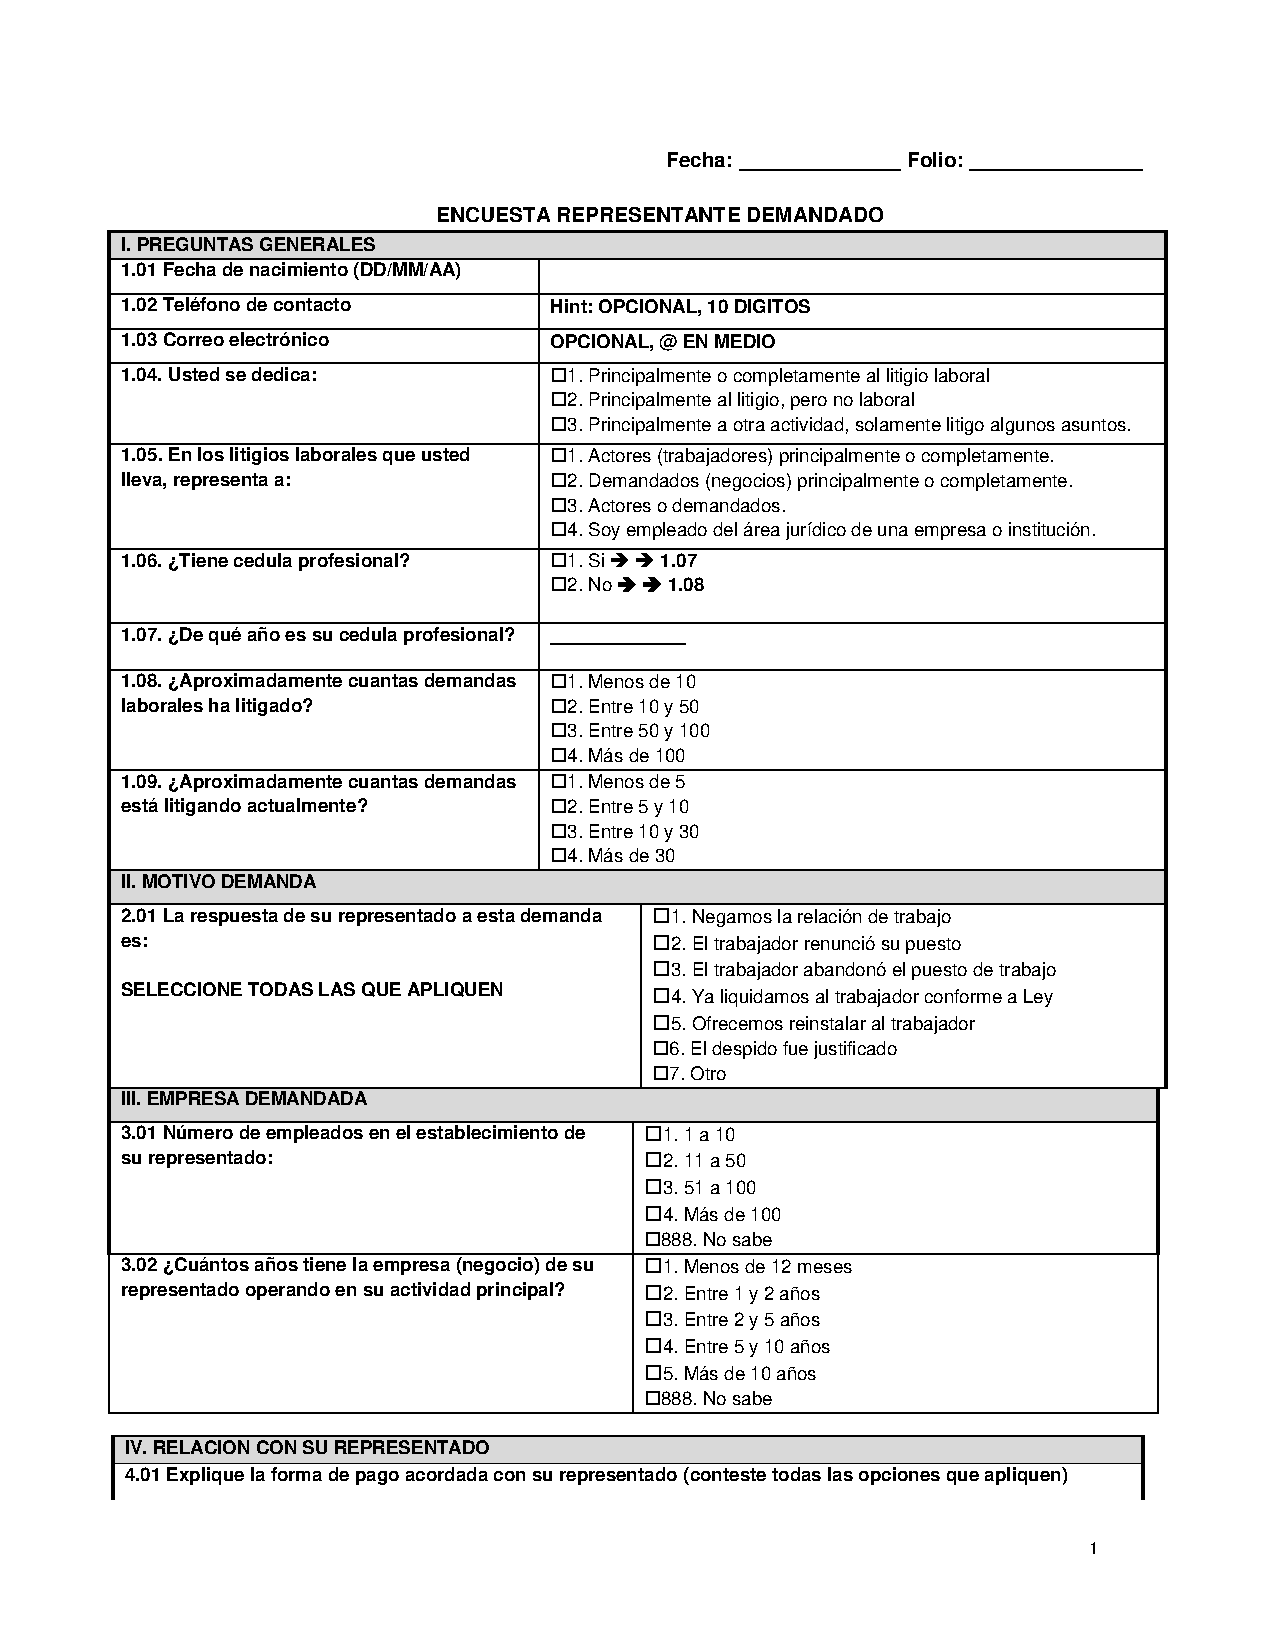
\includepdf[scale=0.8, pages={1-}]{./Surveys/EncuestaACTOR.pdf}
% \end{center}


% \subsection*{Employee's Lawyer}

% \begin{center}
% 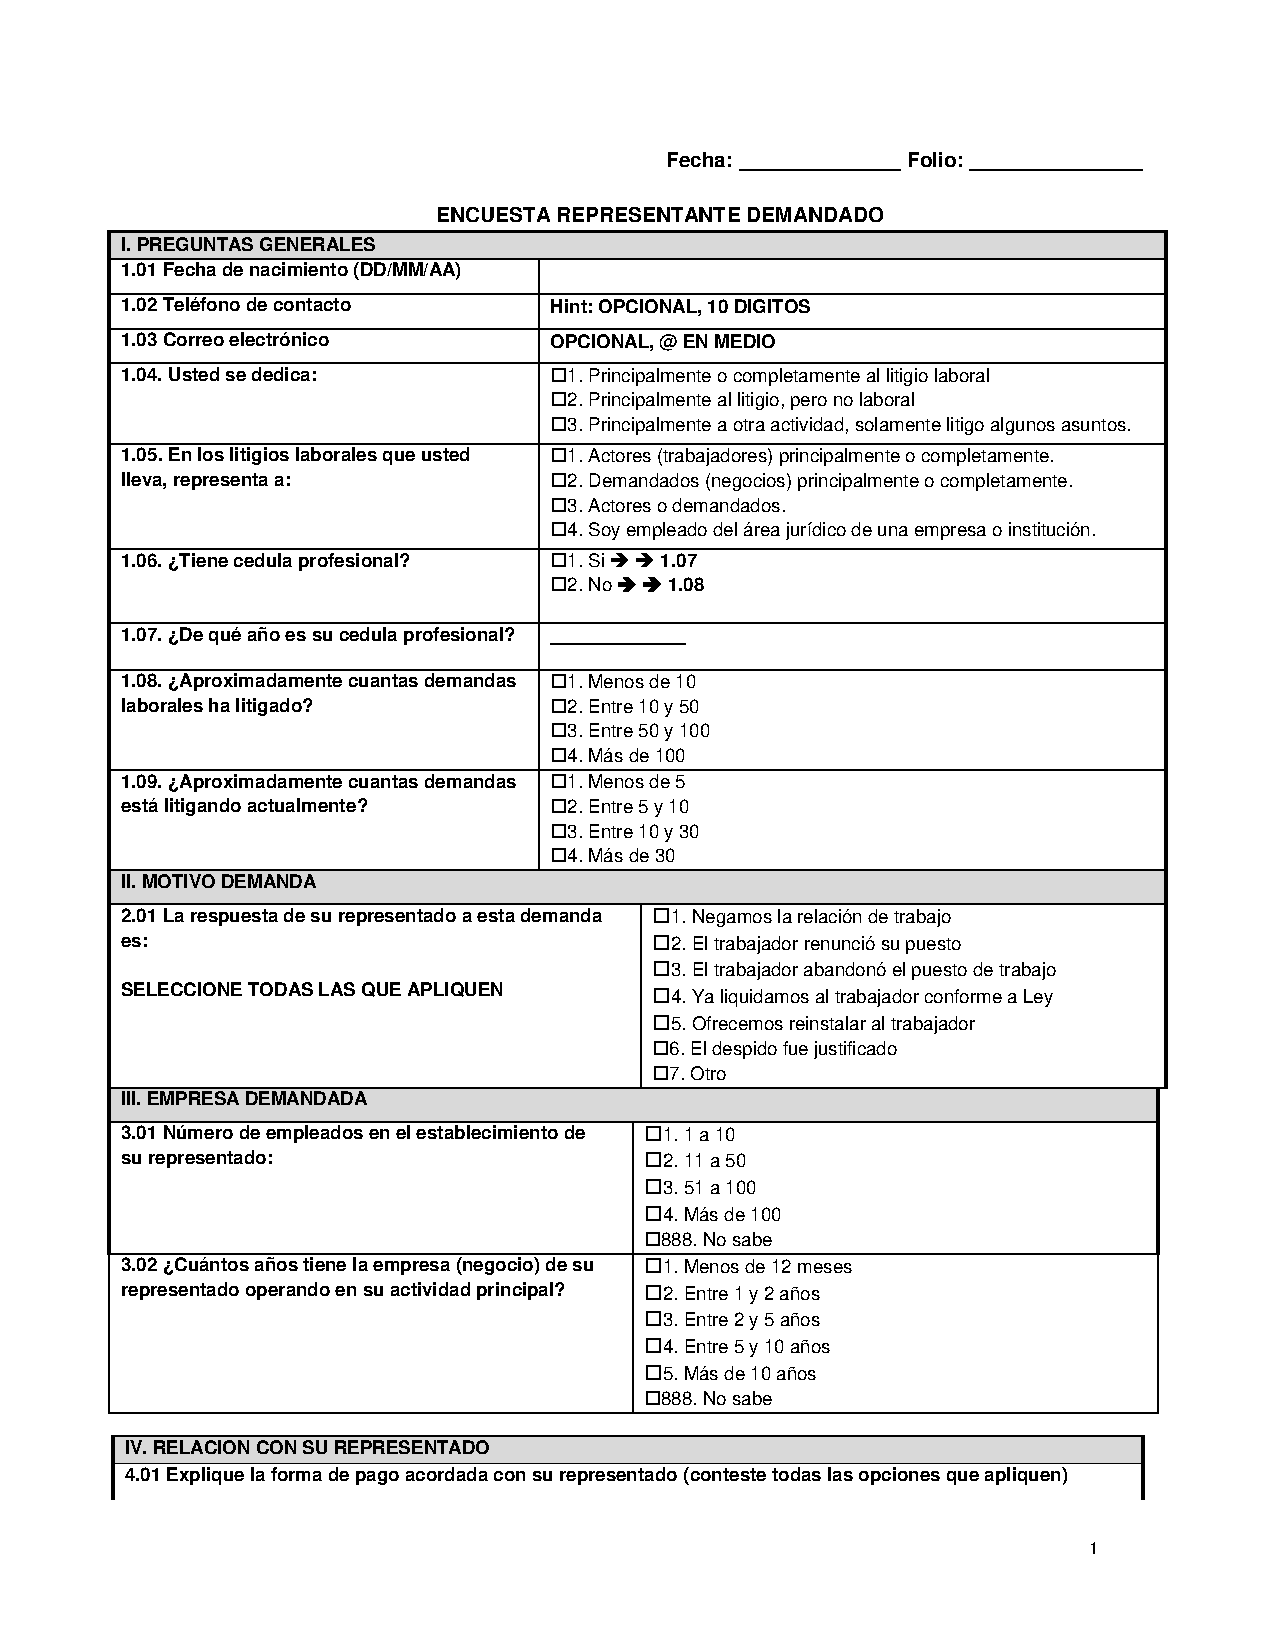
\includepdf[scale=0.8, pages={1-}]{./Surveys/EncuestaREPRESENTANTE_ACTOR.pdf}
% \end{center}

% \subsection*{Firm}

% \begin{center}
% 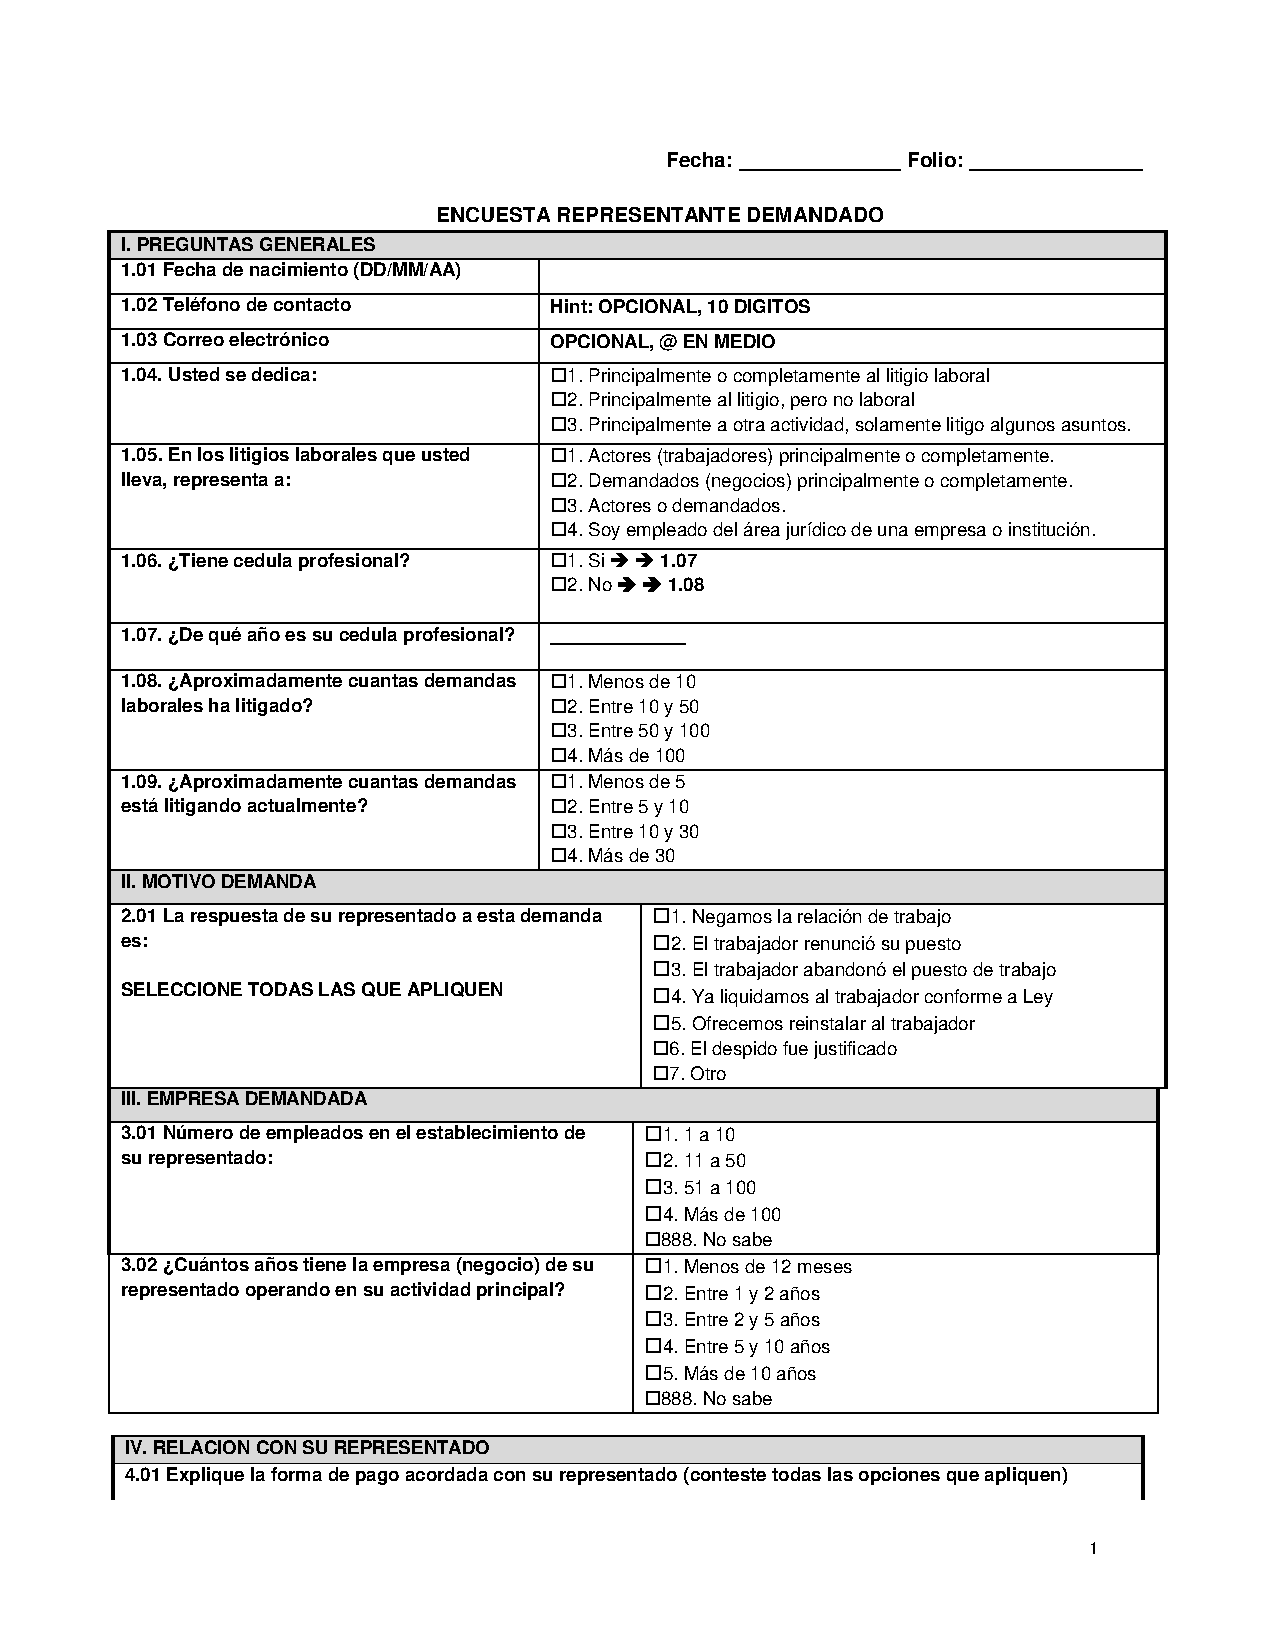
\includepdf[scale=0.8, pages={1-}]{./Surveys/EncuestaDEMANDADO.pdf}
% \end{center}

% \subsection*{Firm's Lawyer}

% \begin{center}
% 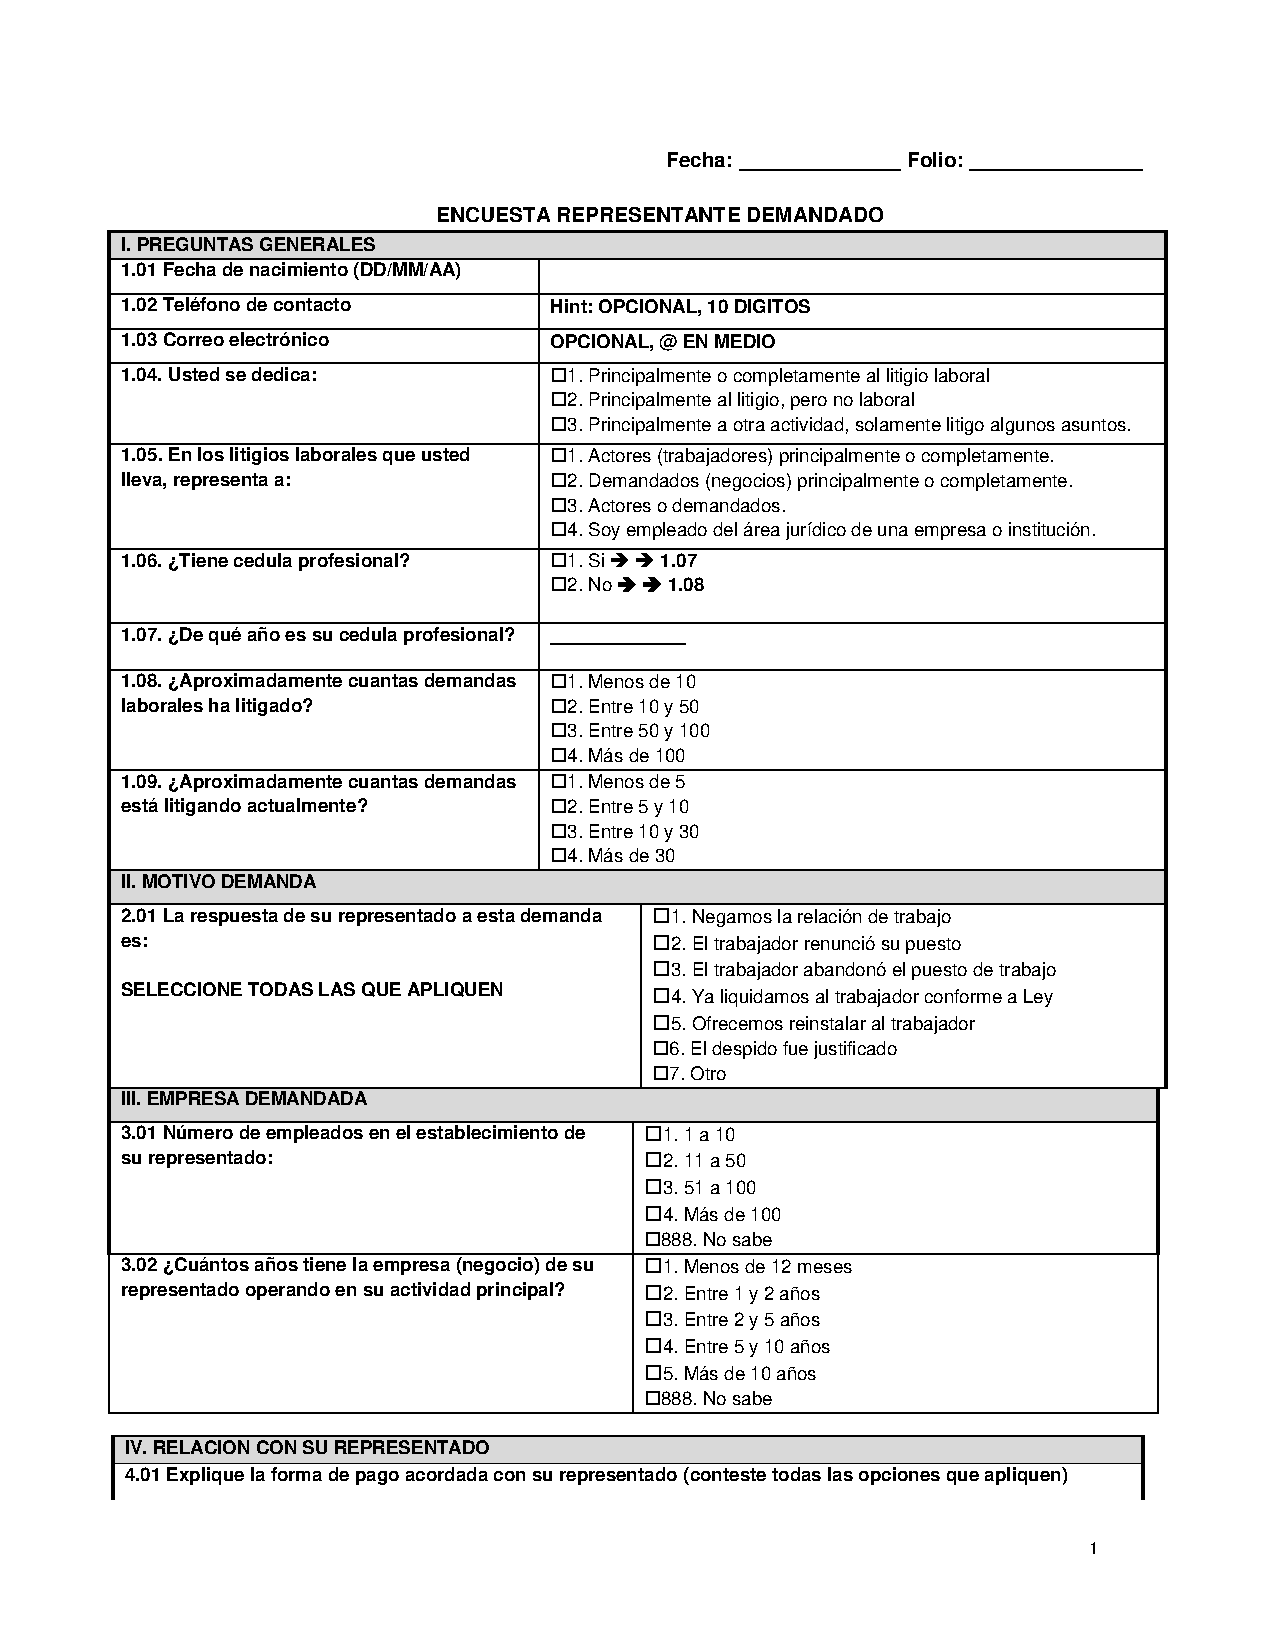
\includepdf[scale=0.8, pages={1-}]{./Surveys/EncuestaREPRESENTANTE_DEMANDADO.pdf}
% \end{center}

% \pagebreak






\end{document}